% **************************************************************************************************************
% A Classic Thesis Style
% An Homage to The Elements of Typographic Style
%
% Copyright (C) 2011 Andr\'e Miede http://www.miede.de
%
% If you like the style then I would appreciate a postcard. My address 
% can be found in the file ClassicThesis.pdf. A collection of the 
% postcards I received so far is available online at 
% http://postcards.miede.de
%
% License:
% This program is free software; you can redistribute it and/or modify
% it under the terms of the GNU General Public License as published by
% the Free Software Foundation; either version 2 of the License, or
% (at your option) any later version.
%
% This program is distributed in the hope that it will be useful,
% but WITHOUT ANY WARRANTY; without even the implied warranty of
% MERCHANTABILITY or FITNESS FOR A PARTICULAR PURPOSE.  See the
% GNU General Public License for more details.
%
% You should have received a copy of the GNU General Public License
% along with this program; see the file COPYING.  If not, write to
% the Free Software Foundation, Inc., 59 Temple Place - Suite 330,
% Boston, MA 02111-1307, USA.
%
% **************************************************************************************************************
% Note:
%    * You must not use "u etc. in strings/commands that will be spaced out (use \"u or real umlauts instead)
%    * New enumeration (small caps): \begin{aenumerate} \end{aenumerate}
%    * For margin notes: \marginpar or \graffito{}
%    * Do not use bold fonts in this style, it is designed around them
%    * Use tables as in the examples
%    * See classicthesis-preamble.sty for useful commands
% **************************************************************************************************************
% To Do:
%		 * [high] Check this out: http://www.golatex.de/koma-script-warnung-in-verbindung-mit-listings-package-t2058.html
%    * [medium] mathbb in section-titles/chapter-titles => disappears somehow in headlines!!!
% **************************************************************************************************************
\documentclass[ twoside,openright,titlepage,numbers=noenddot,headinclude,%1headlines,% letterpaper a4paper
                footinclude=true,cleardoublepage=empty,abstractoff, % <--- obsolete, remove (todo)
                BCOR=5mm,paper=a4,fontsize=12pt,%11pt,a4paper,%
                ngerman,american,%
                ]{scrreprt}

%********************************************************************
% Note: Make all your adjustments in here
%*******************************************************
\usepackage{graphviz}
\usepackage{msctexen}
\usepackage{morewrites} % prevents "No more room for a new \write"

% ****************************************************************************************************
% classicthesis-config.tex 
% formerly known as loadpackages.sty, classicthesis-ldpkg.sty, and classicthesis-preamble.sty 
% Use it at the beginning of your ClassicThesis.tex, or as a LaTeX Preamble 
% in your ClassicThesis.{tex,lyx} with % ****************************************************************************************************
% classicthesis-config.tex 
% formerly known as loadpackages.sty, classicthesis-ldpkg.sty, and classicthesis-preamble.sty 
% Use it at the beginning of your ClassicThesis.tex, or as a LaTeX Preamble 
% in your ClassicThesis.{tex,lyx} with % ****************************************************************************************************
% classicthesis-config.tex 
% formerly known as loadpackages.sty, classicthesis-ldpkg.sty, and classicthesis-preamble.sty 
% Use it at the beginning of your ClassicThesis.tex, or as a LaTeX Preamble 
% in your ClassicThesis.{tex,lyx} with \input{classicthesis-config}
% ****************************************************************************************************  
% If you like the classicthesis, then I would appreciate a postcard. 
% My address can be found in the file ClassicThesis.pdf. A collection 
% of the postcards I received so far is available online at 
% http://postcards.miede.de
% ****************************************************************************************************

% ****************************************************************************************************
% 1. Configure classicthesis for your needs here, e.g., remove "drafting" below 
% in order to deactivate the time-stamp on the pages
% ****************************************************************************************************
\PassOptionsToPackage{eulerchapternumbers,listings,%drafting,%
				 pdfspacing,%floatperchapter,%linedheaders,%
				 subfig,beramono,eulermath,parts}{classicthesis}										
% ********************************************************************
% Available options for classicthesis.sty 
% (see ClassicThesis.pdf for more information):
% drafting
% parts nochapters linedheaders
% eulerchapternumbers beramono eulermath pdfspacing minionprospacing
% tocaligned dottedtoc manychapters
% listings floatperchapter subfig
% ********************************************************************

% ********************************************************************
% Triggers for this config
% ******************************************************************** 
\usepackage{ifthen}
\newboolean{enable-backrefs} % enable backrefs in the bibliography
\setboolean{enable-backrefs}{false} % true false
% ****************************************************************************************************


% ****************************************************************************************************
% 2. Personal data and user ad-hoc commands
% ****************************************************************************************************
\newcommand{\myTitle}{Ontologies for interaction\xspace}
\newcommand{\mySubtitle}{Enabling serendipitous interoperability in smart environments\xspace}
\newcommand{\myDegree}{\xspace}
\newcommand{\myName}{Gerrit Niezen\xspace}
\newcommand{\myProf}{Prof. Loe M.G. Feijs\xspace}
\newcommand{\myOtherProf}{Prof. Panos Markopoulus\xspace}
\newcommand{\mySupervisor}{Dr. Jun Hu\xspace}
\newcommand{\myFaculty}{Department of Industrial Design\xspace}
\newcommand{\myDepartment}{Designed Intelligence research group\xspace}
\newcommand{\myUni}{Eindhoven University of Technology\xspace}
\newcommand{\myLocation}{Eindhoven\xspace}
\newcommand{\myTime}{June 2012\xspace}
\newcommand{\myVersion}{version 1.0\xspace}

% ********************************************************************
% Setup, finetuning, and useful commands
% ********************************************************************
\newcounter{dummy} % necessary for correct hyperlinks (to index, bib, etc.)
\newlength{\abcd} % for ab..z string length calculation
\providecommand{\mLyX}{L\kern-.1667em\lower.25em\hbox{Y}\kern-.125emX\@}
\newcommand{\ie}{i.\,e.}
\newcommand{\Ie}{I.\,e.}
\newcommand{\eg}{e.\,g.}
\newcommand{\Eg}{E.\,g.} 
% ****************************************************************************************************



% ****************************************************************************************************
% 3. Loading some handy packages
% ****************************************************************************************************
% ******************************************************************** 
% Packages with options that might require adjustments
% ******************************************************************** 
\PassOptionsToPackage{latin9}{inputenc}	% latin9 (ISO-8859-9) = latin1+"Euro sign"
 \usepackage{inputenc}				

%\PassOptionsToPackage{ngerman,american}{babel}   % change this to your language(s)
% Spanish languages need extra options in order to work with this template
%\PassOptionsToPackage{spanish,es-lcroman}{babel}
 \usepackage{babel}					

\PassOptionsToPackage{square,numbers}{natbib}
 \usepackage{natbib}				

\PassOptionsToPackage{fleqn}{amsmath}		% math environments and more by the AMS 
 \usepackage{amsmath}

% ******************************************************************** 
% General useful packages
% ******************************************************************** 
%\PassOptionsToPackage{T1}{fontenc} % T2A for cyrillics
\usepackage[T1]{fontenc}                 
\usepackage{xspace} % to get the spacing after macros right  
\usepackage{mparhack} % get marginpar right
\usepackage{fixltx2e} % fixes some LaTeX stuff 
\PassOptionsToPackage{printonlyused,smaller}{acronym}
	\usepackage{acronym} % nice macros for handling all acronyms in the thesis
%\renewcommand*{\acsfont}[1]{\textssc{#1}} % for MinionPro
\renewcommand{\bflabel}[1]{{#1}\hfill} % fix the list of acronyms
% ****************************************************************************************************


% ****************************************************************************************************
% 4. Setup floats: tables, (sub)figures, and captions
% ****************************************************************************************************
\usepackage{tabularx} % better tables
	\setlength{\extrarowheight}{3pt} % increase table row height
\newcommand{\tableheadline}[1]{\multicolumn{1}{c}{\spacedlowsmallcaps{#1}}}
\newcommand{\myfloatalign}{\centering} % to be used with each float for alignment
\usepackage{caption}
\captionsetup{format=hang,font=small}
\usepackage{subfig}  
% ****************************************************************************************************


% ****************************************************************************************************
% 5. Setup code listings
% ****************************************************************************************************
\usepackage{listings} 
%\lstset{emph={trueIndex,root},emphstyle=\color{BlueViolet}}%\underbar} % for special keywords
\lstset{language=[LaTeX]Tex,%C++,
    keywordstyle=\color{RoyalBlue},%\bfseries,
    basicstyle=\small\ttfamily,
    %identifierstyle=\color{NavyBlue},
    commentstyle=\color{Green}\ttfamily,
    stringstyle=\rmfamily,
    numbers=none,%left,%
    numberstyle=\scriptsize,%\tiny
    stepnumber=5,
    numbersep=8pt,
    showstringspaces=false,
    breaklines=true,
    frameround=ftff,
    frame=single,
    belowcaptionskip=.75\baselineskip
    %frame=L
} 
% ****************************************************************************************************    		   


% ****************************************************************************************************
% 6. PDFLaTeX, hyperreferences and citation backreferences
% ****************************************************************************************************
% ********************************************************************
% Using PDFLaTeX
% ********************************************************************
\PassOptionsToPackage{pdftex,hyperfootnotes=false,pdfpagelabels}{hyperref}
	\usepackage{hyperref}  % backref linktocpage pagebackref
\pdfcompresslevel=9
\pdfadjustspacing=1 
\PassOptionsToPackage{pdftex}{graphicx}
	\usepackage{graphicx}
	\graphicspath{{images/}} 

% ********************************************************************
% Setup the style of the backrefs from the bibliography
% (translate the options to any language you use)
% ********************************************************************
\newcommand{\backrefnotcitedstring}{\relax}%(Not cited.)
\newcommand{\backrefcitedsinglestring}[1]{(Cited on page~#1.)}
\newcommand{\backrefcitedmultistring}[1]{(Cited on pages~#1.)}
\ifthenelse{\boolean{enable-backrefs}}%
{%
		\PassOptionsToPackage{hyperpageref}{backref}
		\usepackage{backref} % to be loaded after hyperref package 
		   \renewcommand{\backreftwosep}{ and~} % separate 2 pages
		   \renewcommand{\backreflastsep}{, and~} % separate last of longer list
		   \renewcommand*{\backref}[1]{}  % disable standard
		   \renewcommand*{\backrefalt}[4]{% detailed backref
		      \ifcase #1 %
		         \backrefnotcitedstring%
		      \or%
		         \backrefcitedsinglestring{#2}%
		      \else%
		         \backrefcitedmultistring{#2}%
		      \fi}%
}{\relax}    

% ********************************************************************
% Hyperreferences
% ********************************************************************
\hypersetup{%
    %draft,	% = no hyperlinking at all (useful in b/w printouts)
    colorlinks=true, linktocpage=true, pdfstartpage=3, pdfstartview=FitV,%
    % uncomment the following line if you want to have black links (e.g., for printing)
    %colorlinks=false, linktocpage=false, pdfborder={0 0 0}, pdfstartpage=3, pdfstartview=FitV,% 
    breaklinks=true, pdfpagemode=UseNone, pageanchor=true, pdfpagemode=UseOutlines,%
    plainpages=false, bookmarksnumbered, bookmarksopen=true, bookmarksopenlevel=1,%
    hypertexnames=true, pdfhighlight=/O,%nesting=true,%frenchlinks,%
    urlcolor=webbrown, linkcolor=RoyalBlue, citecolor=webgreen, %pagecolor=RoyalBlue,%
    %urlcolor=Black, linkcolor=Black, citecolor=Black, %pagecolor=Black,%
    pdftitle={\myTitle},%
    pdfauthor={\textcopyright\ \myName, \myUni, \myFaculty},%
    pdfsubject={},%
    pdfkeywords={},%
    pdfcreator={pdfLaTeX},%
    pdfproducer={LaTeX with hyperref and classicthesis}%
}   

% ********************************************************************
% Setup autoreferences
% ********************************************************************
% There are some issues regarding autorefnames
% http://www.ureader.de/msg/136221647.aspx
% http://www.tex.ac.uk/cgi-bin/texfaq2html?label=latexwords
% you have to redefine the makros for the 
% language you use, e.g., american, ngerman
% (as chosen when loading babel/AtBeginDocument)
% ********************************************************************
\makeatletter
\@ifpackageloaded{babel}%
    {%
       \addto\extrasamerican{%
					\renewcommand*{\figureautorefname}{Figure}%
					\renewcommand*{\tableautorefname}{Table}%
					\renewcommand*{\partautorefname}{Part}%
					\renewcommand*{\chapterautorefname}{Chapter}%
					\renewcommand*{\sectionautorefname}{Section}%
					\renewcommand*{\subsectionautorefname}{Section}%
					\renewcommand*{\subsubsectionautorefname}{Section}% 	
				}%
       \addto\extrasngerman{% 
					\renewcommand*{\paragraphautorefname}{Absatz}%
					\renewcommand*{\subparagraphautorefname}{Unterabsatz}%
					\renewcommand*{\footnoteautorefname}{Fu\"snote}%
					\renewcommand*{\FancyVerbLineautorefname}{Zeile}%
					\renewcommand*{\theoremautorefname}{Theorem}%
					\renewcommand*{\appendixautorefname}{Anhang}%
					\renewcommand*{\equationautorefname}{Gleichung}%        
					\renewcommand*{\itemautorefname}{Punkt}%
				}%	
			% Fix to getting autorefs for subfigures right (thanks to Belinda Vogt for changing the definition)
			\providecommand{\subfigureautorefname}{\figureautorefname}%  			
    }{\relax}
\makeatother


% ****************************************************************************************************
% 7. Last calls before the bar closes
% ****************************************************************************************************
% ********************************************************************
% Development Stuff
% ********************************************************************
\listfiles
%\PassOptionsToPackage{l2tabu,orthodox,abort}{nag}
%	\usepackage{nag}
%\PassOptionsToPackage{warning, all}{onlyamsmath}
%	\usepackage{onlyamsmath}

% ********************************************************************
% Last, but not least...
% ********************************************************************
\usepackage{classicthesis} 
% ****************************************************************************************************


% ****************************************************************************************************
% 8. Further adjustments (experimental)
% ****************************************************************************************************
% ********************************************************************
% Changing the text area
% ********************************************************************
%\linespread{1.05} % a bit more for Palatino
%\areaset[current]{312pt}{761pt} % 686 (factor 2.2) + 33 head + 42 head \the\footskip
%\setlength{\marginparwidth}{7em}%
%\setlength{\marginparsep}{2em}%

% ********************************************************************
% Using different fonts
% ********************************************************************
%\usepackage[oldstylenums]{kpfonts} % oldstyle notextcomp
%\usepackage[osf]{libertine}
%\usepackage{hfoldsty} % Computer Modern with osf
%\usepackage[light,condensed,math]{iwona}
%\renewcommand{\sfdefault}{iwona}
%\usepackage{lmodern} % <-- no osf support :-(
%\usepackage[urw-garamond]{mathdesign} <-- no osf support :-(
% ****************************************************************************************************

% ****************************************************************************************************  
% If you like the classicthesis, then I would appreciate a postcard. 
% My address can be found in the file ClassicThesis.pdf. A collection 
% of the postcards I received so far is available online at 
% http://postcards.miede.de
% ****************************************************************************************************

% ****************************************************************************************************
% 1. Configure classicthesis for your needs here, e.g., remove "drafting" below 
% in order to deactivate the time-stamp on the pages
% ****************************************************************************************************
\PassOptionsToPackage{eulerchapternumbers,listings,%drafting,%
				 pdfspacing,%floatperchapter,%linedheaders,%
				 subfig,beramono,eulermath,parts}{classicthesis}										
% ********************************************************************
% Available options for classicthesis.sty 
% (see ClassicThesis.pdf for more information):
% drafting
% parts nochapters linedheaders
% eulerchapternumbers beramono eulermath pdfspacing minionprospacing
% tocaligned dottedtoc manychapters
% listings floatperchapter subfig
% ********************************************************************

% ********************************************************************
% Triggers for this config
% ******************************************************************** 
\usepackage{ifthen}
\newboolean{enable-backrefs} % enable backrefs in the bibliography
\setboolean{enable-backrefs}{false} % true false
% ****************************************************************************************************


% ****************************************************************************************************
% 2. Personal data and user ad-hoc commands
% ****************************************************************************************************
\newcommand{\myTitle}{Ontologies for interaction\xspace}
\newcommand{\mySubtitle}{Enabling serendipitous interoperability in smart environments\xspace}
\newcommand{\myDegree}{\xspace}
\newcommand{\myName}{Gerrit Niezen\xspace}
\newcommand{\myProf}{Prof. Loe M.G. Feijs\xspace}
\newcommand{\myOtherProf}{Prof. Panos Markopoulus\xspace}
\newcommand{\mySupervisor}{Dr. Jun Hu\xspace}
\newcommand{\myFaculty}{Department of Industrial Design\xspace}
\newcommand{\myDepartment}{Designed Intelligence research group\xspace}
\newcommand{\myUni}{Eindhoven University of Technology\xspace}
\newcommand{\myLocation}{Eindhoven\xspace}
\newcommand{\myTime}{June 2012\xspace}
\newcommand{\myVersion}{version 1.0\xspace}

% ********************************************************************
% Setup, finetuning, and useful commands
% ********************************************************************
\newcounter{dummy} % necessary for correct hyperlinks (to index, bib, etc.)
\newlength{\abcd} % for ab..z string length calculation
\providecommand{\mLyX}{L\kern-.1667em\lower.25em\hbox{Y}\kern-.125emX\@}
\newcommand{\ie}{i.\,e.}
\newcommand{\Ie}{I.\,e.}
\newcommand{\eg}{e.\,g.}
\newcommand{\Eg}{E.\,g.} 
% ****************************************************************************************************



% ****************************************************************************************************
% 3. Loading some handy packages
% ****************************************************************************************************
% ******************************************************************** 
% Packages with options that might require adjustments
% ******************************************************************** 
\PassOptionsToPackage{latin9}{inputenc}	% latin9 (ISO-8859-9) = latin1+"Euro sign"
 \usepackage{inputenc}				

%\PassOptionsToPackage{ngerman,american}{babel}   % change this to your language(s)
% Spanish languages need extra options in order to work with this template
%\PassOptionsToPackage{spanish,es-lcroman}{babel}
 \usepackage{babel}					

\PassOptionsToPackage{square,numbers}{natbib}
 \usepackage{natbib}				

\PassOptionsToPackage{fleqn}{amsmath}		% math environments and more by the AMS 
 \usepackage{amsmath}

% ******************************************************************** 
% General useful packages
% ******************************************************************** 
%\PassOptionsToPackage{T1}{fontenc} % T2A for cyrillics
\usepackage[T1]{fontenc}                 
\usepackage{xspace} % to get the spacing after macros right  
\usepackage{mparhack} % get marginpar right
\usepackage{fixltx2e} % fixes some LaTeX stuff 
\PassOptionsToPackage{printonlyused,smaller}{acronym}
	\usepackage{acronym} % nice macros for handling all acronyms in the thesis
%\renewcommand*{\acsfont}[1]{\textssc{#1}} % for MinionPro
\renewcommand{\bflabel}[1]{{#1}\hfill} % fix the list of acronyms
% ****************************************************************************************************


% ****************************************************************************************************
% 4. Setup floats: tables, (sub)figures, and captions
% ****************************************************************************************************
\usepackage{tabularx} % better tables
	\setlength{\extrarowheight}{3pt} % increase table row height
\newcommand{\tableheadline}[1]{\multicolumn{1}{c}{\spacedlowsmallcaps{#1}}}
\newcommand{\myfloatalign}{\centering} % to be used with each float for alignment
\usepackage{caption}
\captionsetup{format=hang,font=small}
\usepackage{subfig}  
% ****************************************************************************************************


% ****************************************************************************************************
% 5. Setup code listings
% ****************************************************************************************************
\usepackage{listings} 
%\lstset{emph={trueIndex,root},emphstyle=\color{BlueViolet}}%\underbar} % for special keywords
\lstset{language=[LaTeX]Tex,%C++,
    keywordstyle=\color{RoyalBlue},%\bfseries,
    basicstyle=\small\ttfamily,
    %identifierstyle=\color{NavyBlue},
    commentstyle=\color{Green}\ttfamily,
    stringstyle=\rmfamily,
    numbers=none,%left,%
    numberstyle=\scriptsize,%\tiny
    stepnumber=5,
    numbersep=8pt,
    showstringspaces=false,
    breaklines=true,
    frameround=ftff,
    frame=single,
    belowcaptionskip=.75\baselineskip
    %frame=L
} 
% ****************************************************************************************************    		   


% ****************************************************************************************************
% 6. PDFLaTeX, hyperreferences and citation backreferences
% ****************************************************************************************************
% ********************************************************************
% Using PDFLaTeX
% ********************************************************************
\PassOptionsToPackage{pdftex,hyperfootnotes=false,pdfpagelabels}{hyperref}
	\usepackage{hyperref}  % backref linktocpage pagebackref
\pdfcompresslevel=9
\pdfadjustspacing=1 
\PassOptionsToPackage{pdftex}{graphicx}
	\usepackage{graphicx}
	\graphicspath{{images/}} 

% ********************************************************************
% Setup the style of the backrefs from the bibliography
% (translate the options to any language you use)
% ********************************************************************
\newcommand{\backrefnotcitedstring}{\relax}%(Not cited.)
\newcommand{\backrefcitedsinglestring}[1]{(Cited on page~#1.)}
\newcommand{\backrefcitedmultistring}[1]{(Cited on pages~#1.)}
\ifthenelse{\boolean{enable-backrefs}}%
{%
		\PassOptionsToPackage{hyperpageref}{backref}
		\usepackage{backref} % to be loaded after hyperref package 
		   \renewcommand{\backreftwosep}{ and~} % separate 2 pages
		   \renewcommand{\backreflastsep}{, and~} % separate last of longer list
		   \renewcommand*{\backref}[1]{}  % disable standard
		   \renewcommand*{\backrefalt}[4]{% detailed backref
		      \ifcase #1 %
		         \backrefnotcitedstring%
		      \or%
		         \backrefcitedsinglestring{#2}%
		      \else%
		         \backrefcitedmultistring{#2}%
		      \fi}%
}{\relax}    

% ********************************************************************
% Hyperreferences
% ********************************************************************
\hypersetup{%
    %draft,	% = no hyperlinking at all (useful in b/w printouts)
    colorlinks=true, linktocpage=true, pdfstartpage=3, pdfstartview=FitV,%
    % uncomment the following line if you want to have black links (e.g., for printing)
    %colorlinks=false, linktocpage=false, pdfborder={0 0 0}, pdfstartpage=3, pdfstartview=FitV,% 
    breaklinks=true, pdfpagemode=UseNone, pageanchor=true, pdfpagemode=UseOutlines,%
    plainpages=false, bookmarksnumbered, bookmarksopen=true, bookmarksopenlevel=1,%
    hypertexnames=true, pdfhighlight=/O,%nesting=true,%frenchlinks,%
    urlcolor=webbrown, linkcolor=RoyalBlue, citecolor=webgreen, %pagecolor=RoyalBlue,%
    %urlcolor=Black, linkcolor=Black, citecolor=Black, %pagecolor=Black,%
    pdftitle={\myTitle},%
    pdfauthor={\textcopyright\ \myName, \myUni, \myFaculty},%
    pdfsubject={},%
    pdfkeywords={},%
    pdfcreator={pdfLaTeX},%
    pdfproducer={LaTeX with hyperref and classicthesis}%
}   

% ********************************************************************
% Setup autoreferences
% ********************************************************************
% There are some issues regarding autorefnames
% http://www.ureader.de/msg/136221647.aspx
% http://www.tex.ac.uk/cgi-bin/texfaq2html?label=latexwords
% you have to redefine the makros for the 
% language you use, e.g., american, ngerman
% (as chosen when loading babel/AtBeginDocument)
% ********************************************************************
\makeatletter
\@ifpackageloaded{babel}%
    {%
       \addto\extrasamerican{%
					\renewcommand*{\figureautorefname}{Figure}%
					\renewcommand*{\tableautorefname}{Table}%
					\renewcommand*{\partautorefname}{Part}%
					\renewcommand*{\chapterautorefname}{Chapter}%
					\renewcommand*{\sectionautorefname}{Section}%
					\renewcommand*{\subsectionautorefname}{Section}%
					\renewcommand*{\subsubsectionautorefname}{Section}% 	
				}%
       \addto\extrasngerman{% 
					\renewcommand*{\paragraphautorefname}{Absatz}%
					\renewcommand*{\subparagraphautorefname}{Unterabsatz}%
					\renewcommand*{\footnoteautorefname}{Fu\"snote}%
					\renewcommand*{\FancyVerbLineautorefname}{Zeile}%
					\renewcommand*{\theoremautorefname}{Theorem}%
					\renewcommand*{\appendixautorefname}{Anhang}%
					\renewcommand*{\equationautorefname}{Gleichung}%        
					\renewcommand*{\itemautorefname}{Punkt}%
				}%	
			% Fix to getting autorefs for subfigures right (thanks to Belinda Vogt for changing the definition)
			\providecommand{\subfigureautorefname}{\figureautorefname}%  			
    }{\relax}
\makeatother


% ****************************************************************************************************
% 7. Last calls before the bar closes
% ****************************************************************************************************
% ********************************************************************
% Development Stuff
% ********************************************************************
\listfiles
%\PassOptionsToPackage{l2tabu,orthodox,abort}{nag}
%	\usepackage{nag}
%\PassOptionsToPackage{warning, all}{onlyamsmath}
%	\usepackage{onlyamsmath}

% ********************************************************************
% Last, but not least...
% ********************************************************************
\usepackage{classicthesis} 
% ****************************************************************************************************


% ****************************************************************************************************
% 8. Further adjustments (experimental)
% ****************************************************************************************************
% ********************************************************************
% Changing the text area
% ********************************************************************
%\linespread{1.05} % a bit more for Palatino
%\areaset[current]{312pt}{761pt} % 686 (factor 2.2) + 33 head + 42 head \the\footskip
%\setlength{\marginparwidth}{7em}%
%\setlength{\marginparsep}{2em}%

% ********************************************************************
% Using different fonts
% ********************************************************************
%\usepackage[oldstylenums]{kpfonts} % oldstyle notextcomp
%\usepackage[osf]{libertine}
%\usepackage{hfoldsty} % Computer Modern with osf
%\usepackage[light,condensed,math]{iwona}
%\renewcommand{\sfdefault}{iwona}
%\usepackage{lmodern} % <-- no osf support :-(
%\usepackage[urw-garamond]{mathdesign} <-- no osf support :-(
% ****************************************************************************************************

% ****************************************************************************************************  
% If you like the classicthesis, then I would appreciate a postcard. 
% My address can be found in the file ClassicThesis.pdf. A collection 
% of the postcards I received so far is available online at 
% http://postcards.miede.de
% ****************************************************************************************************

% ****************************************************************************************************
% 1. Configure classicthesis for your needs here, e.g., remove "drafting" below 
% in order to deactivate the time-stamp on the pages
% ****************************************************************************************************
\PassOptionsToPackage{eulerchapternumbers,listings,%drafting,%
				 pdfspacing,%floatperchapter,%linedheaders,%
				 subfig,beramono,eulermath,parts}{classicthesis}										
% ********************************************************************
% Available options for classicthesis.sty 
% (see ClassicThesis.pdf for more information):
% drafting
% parts nochapters linedheaders
% eulerchapternumbers beramono eulermath pdfspacing minionprospacing
% tocaligned dottedtoc manychapters
% listings floatperchapter subfig
% ********************************************************************

% ********************************************************************
% Triggers for this config
% ******************************************************************** 
\usepackage{ifthen}
\newboolean{enable-backrefs} % enable backrefs in the bibliography
\setboolean{enable-backrefs}{false} % true false
% ****************************************************************************************************


% ****************************************************************************************************
% 2. Personal data and user ad-hoc commands
% ****************************************************************************************************
\newcommand{\myTitle}{Ontologies for interaction\xspace}
\newcommand{\mySubtitle}{Enabling serendipitous interoperability in smart environments\xspace}
\newcommand{\myDegree}{\xspace}
\newcommand{\myName}{Gerrit Niezen\xspace}
\newcommand{\myProf}{Prof. Loe M.G. Feijs\xspace}
\newcommand{\myOtherProf}{Prof. Panos Markopoulus\xspace}
\newcommand{\mySupervisor}{Dr. Jun Hu\xspace}
\newcommand{\myFaculty}{Department of Industrial Design\xspace}
\newcommand{\myDepartment}{Designed Intelligence research group\xspace}
\newcommand{\myUni}{Eindhoven University of Technology\xspace}
\newcommand{\myLocation}{Eindhoven\xspace}
\newcommand{\myTime}{June 2012\xspace}
\newcommand{\myVersion}{version 1.0\xspace}

% ********************************************************************
% Setup, finetuning, and useful commands
% ********************************************************************
\newcounter{dummy} % necessary for correct hyperlinks (to index, bib, etc.)
\newlength{\abcd} % for ab..z string length calculation
\providecommand{\mLyX}{L\kern-.1667em\lower.25em\hbox{Y}\kern-.125emX\@}
\newcommand{\ie}{i.\,e.}
\newcommand{\Ie}{I.\,e.}
\newcommand{\eg}{e.\,g.}
\newcommand{\Eg}{E.\,g.} 
% ****************************************************************************************************



% ****************************************************************************************************
% 3. Loading some handy packages
% ****************************************************************************************************
% ******************************************************************** 
% Packages with options that might require adjustments
% ******************************************************************** 
\PassOptionsToPackage{latin9}{inputenc}	% latin9 (ISO-8859-9) = latin1+"Euro sign"
 \usepackage{inputenc}				

%\PassOptionsToPackage{ngerman,american}{babel}   % change this to your language(s)
% Spanish languages need extra options in order to work with this template
%\PassOptionsToPackage{spanish,es-lcroman}{babel}
 \usepackage{babel}					

\PassOptionsToPackage{square,numbers}{natbib}
 \usepackage{natbib}				

\PassOptionsToPackage{fleqn}{amsmath}		% math environments and more by the AMS 
 \usepackage{amsmath}

% ******************************************************************** 
% General useful packages
% ******************************************************************** 
%\PassOptionsToPackage{T1}{fontenc} % T2A for cyrillics
\usepackage[T1]{fontenc}                 
\usepackage{xspace} % to get the spacing after macros right  
\usepackage{mparhack} % get marginpar right
\usepackage{fixltx2e} % fixes some LaTeX stuff 
\PassOptionsToPackage{printonlyused,smaller}{acronym}
	\usepackage{acronym} % nice macros for handling all acronyms in the thesis
%\renewcommand*{\acsfont}[1]{\textssc{#1}} % for MinionPro
\renewcommand{\bflabel}[1]{{#1}\hfill} % fix the list of acronyms
% ****************************************************************************************************


% ****************************************************************************************************
% 4. Setup floats: tables, (sub)figures, and captions
% ****************************************************************************************************
\usepackage{tabularx} % better tables
	\setlength{\extrarowheight}{3pt} % increase table row height
\newcommand{\tableheadline}[1]{\multicolumn{1}{c}{\spacedlowsmallcaps{#1}}}
\newcommand{\myfloatalign}{\centering} % to be used with each float for alignment
\usepackage{caption}
\captionsetup{format=hang,font=small}
\usepackage{subfig}  
% ****************************************************************************************************


% ****************************************************************************************************
% 5. Setup code listings
% ****************************************************************************************************
\usepackage{listings} 
%\lstset{emph={trueIndex,root},emphstyle=\color{BlueViolet}}%\underbar} % for special keywords
\lstset{language=[LaTeX]Tex,%C++,
    keywordstyle=\color{RoyalBlue},%\bfseries,
    basicstyle=\small\ttfamily,
    %identifierstyle=\color{NavyBlue},
    commentstyle=\color{Green}\ttfamily,
    stringstyle=\rmfamily,
    numbers=none,%left,%
    numberstyle=\scriptsize,%\tiny
    stepnumber=5,
    numbersep=8pt,
    showstringspaces=false,
    breaklines=true,
    frameround=ftff,
    frame=single,
    belowcaptionskip=.75\baselineskip
    %frame=L
} 
% ****************************************************************************************************    		   


% ****************************************************************************************************
% 6. PDFLaTeX, hyperreferences and citation backreferences
% ****************************************************************************************************
% ********************************************************************
% Using PDFLaTeX
% ********************************************************************
\PassOptionsToPackage{pdftex,hyperfootnotes=false,pdfpagelabels}{hyperref}
	\usepackage{hyperref}  % backref linktocpage pagebackref
\pdfcompresslevel=9
\pdfadjustspacing=1 
\PassOptionsToPackage{pdftex}{graphicx}
	\usepackage{graphicx}
	\graphicspath{{images/}} 

% ********************************************************************
% Setup the style of the backrefs from the bibliography
% (translate the options to any language you use)
% ********************************************************************
\newcommand{\backrefnotcitedstring}{\relax}%(Not cited.)
\newcommand{\backrefcitedsinglestring}[1]{(Cited on page~#1.)}
\newcommand{\backrefcitedmultistring}[1]{(Cited on pages~#1.)}
\ifthenelse{\boolean{enable-backrefs}}%
{%
		\PassOptionsToPackage{hyperpageref}{backref}
		\usepackage{backref} % to be loaded after hyperref package 
		   \renewcommand{\backreftwosep}{ and~} % separate 2 pages
		   \renewcommand{\backreflastsep}{, and~} % separate last of longer list
		   \renewcommand*{\backref}[1]{}  % disable standard
		   \renewcommand*{\backrefalt}[4]{% detailed backref
		      \ifcase #1 %
		         \backrefnotcitedstring%
		      \or%
		         \backrefcitedsinglestring{#2}%
		      \else%
		         \backrefcitedmultistring{#2}%
		      \fi}%
}{\relax}    

% ********************************************************************
% Hyperreferences
% ********************************************************************
\hypersetup{%
    %draft,	% = no hyperlinking at all (useful in b/w printouts)
    colorlinks=true, linktocpage=true, pdfstartpage=3, pdfstartview=FitV,%
    % uncomment the following line if you want to have black links (e.g., for printing)
    %colorlinks=false, linktocpage=false, pdfborder={0 0 0}, pdfstartpage=3, pdfstartview=FitV,% 
    breaklinks=true, pdfpagemode=UseNone, pageanchor=true, pdfpagemode=UseOutlines,%
    plainpages=false, bookmarksnumbered, bookmarksopen=true, bookmarksopenlevel=1,%
    hypertexnames=true, pdfhighlight=/O,%nesting=true,%frenchlinks,%
    urlcolor=webbrown, linkcolor=RoyalBlue, citecolor=webgreen, %pagecolor=RoyalBlue,%
    %urlcolor=Black, linkcolor=Black, citecolor=Black, %pagecolor=Black,%
    pdftitle={\myTitle},%
    pdfauthor={\textcopyright\ \myName, \myUni, \myFaculty},%
    pdfsubject={},%
    pdfkeywords={},%
    pdfcreator={pdfLaTeX},%
    pdfproducer={LaTeX with hyperref and classicthesis}%
}   

% ********************************************************************
% Setup autoreferences
% ********************************************************************
% There are some issues regarding autorefnames
% http://www.ureader.de/msg/136221647.aspx
% http://www.tex.ac.uk/cgi-bin/texfaq2html?label=latexwords
% you have to redefine the makros for the 
% language you use, e.g., american, ngerman
% (as chosen when loading babel/AtBeginDocument)
% ********************************************************************
\makeatletter
\@ifpackageloaded{babel}%
    {%
       \addto\extrasamerican{%
					\renewcommand*{\figureautorefname}{Figure}%
					\renewcommand*{\tableautorefname}{Table}%
					\renewcommand*{\partautorefname}{Part}%
					\renewcommand*{\chapterautorefname}{Chapter}%
					\renewcommand*{\sectionautorefname}{Section}%
					\renewcommand*{\subsectionautorefname}{Section}%
					\renewcommand*{\subsubsectionautorefname}{Section}% 	
				}%
       \addto\extrasngerman{% 
					\renewcommand*{\paragraphautorefname}{Absatz}%
					\renewcommand*{\subparagraphautorefname}{Unterabsatz}%
					\renewcommand*{\footnoteautorefname}{Fu\"snote}%
					\renewcommand*{\FancyVerbLineautorefname}{Zeile}%
					\renewcommand*{\theoremautorefname}{Theorem}%
					\renewcommand*{\appendixautorefname}{Anhang}%
					\renewcommand*{\equationautorefname}{Gleichung}%        
					\renewcommand*{\itemautorefname}{Punkt}%
				}%	
			% Fix to getting autorefs for subfigures right (thanks to Belinda Vogt for changing the definition)
			\providecommand{\subfigureautorefname}{\figureautorefname}%  			
    }{\relax}
\makeatother


% ****************************************************************************************************
% 7. Last calls before the bar closes
% ****************************************************************************************************
% ********************************************************************
% Development Stuff
% ********************************************************************
\listfiles
%\PassOptionsToPackage{l2tabu,orthodox,abort}{nag}
%	\usepackage{nag}
%\PassOptionsToPackage{warning, all}{onlyamsmath}
%	\usepackage{onlyamsmath}

% ********************************************************************
% Last, but not least...
% ********************************************************************
\usepackage{classicthesis} 
% ****************************************************************************************************


% ****************************************************************************************************
% 8. Further adjustments (experimental)
% ****************************************************************************************************
% ********************************************************************
% Changing the text area
% ********************************************************************
%\linespread{1.05} % a bit more for Palatino
%\areaset[current]{312pt}{761pt} % 686 (factor 2.2) + 33 head + 42 head \the\footskip
%\setlength{\marginparwidth}{7em}%
%\setlength{\marginparsep}{2em}%

% ********************************************************************
% Using different fonts
% ********************************************************************
%\usepackage[oldstylenums]{kpfonts} % oldstyle notextcomp
%\usepackage[osf]{libertine}
%\usepackage{hfoldsty} % Computer Modern with osf
%\usepackage[light,condensed,math]{iwona}
%\renewcommand{\sfdefault}{iwona}
%\usepackage{lmodern} % <-- no osf support :-(
%\usepackage[urw-garamond]{mathdesign} <-- no osf support :-(
% ****************************************************************************************************


\DeclareGraphicsExtensions{.pdf,.jpeg,.png,.jpg}
\usepackage{minted, caption}
\usemintedstyle{pastie}

\usepackage{multirow}
\usepackage{eurosym}
\usepackage{textcomp} % prevents font warnings like OMS/pplj/m/n on textbullet

\usepackage[absolute]{textpos}

\usepackage{amsthm}
\newtheorem{example}{Example}
\newtheorem{question}{Research question}
\newtheorem{cdquestion}{Question}
 
% \usepackage{multibib}
% \newcites{mypub}{List of publications}




%\includeonly{Chapters/Introduction}
%\includeonly{Chapters/RelatedWork}
%\includeonly{Chapters/DesignIteration1}
%\includeonly{Chapters/DesignIteration2}
%\includeonly{Chapters/DesignIteration3}
%\includeonly{Chapters/SemanticConnectionsTheory}
%\includeonly{Chapters/DeviceCapabilityModelling}
%\includeonly{Chapters/EventModelling}
%\includeonly{Chapters/OntologyEngineering}
%\includeonly{Chapters/SoftwareArchitecture}
%\includeonly{Chapters/Evaluation}
%\includeonly{Chapters/Conclusion}

%********************************************************************
% Hyphenation
%*******************************************************
%\hyphenation{hu-man}
\hyphenation{Mi-cro-soft}


% ********************************************************************
% GO!GO!GO! MOVE IT!
%*******************************************************
\begin{document}
\frenchspacing
\raggedbottom
\selectlanguage{american} % american ngerman
%\renewcommand*{\bibname}{new name}
%\setbibpreamble{}
\pagenumbering{roman}
\pagestyle{plain}
%********************************************************************
% Frontmatter
%*******************************************************
%%*******************************************************
% Little Dirty Titlepage
%*******************************************************
\thispagestyle{empty}
%\pdfbookmark[1]{Titel}{title}
%*******************************************************
\begin{center}
    \spacedlowsmallcaps{\myName} \\ \medskip                        

    \begingroup
        %\color{Maroon}
		\spacedallcaps{\myTitle}
    \endgroup
\end{center}        

%*******************************************************
% Titlepage
%*******************************************************
\begin{titlepage}
	% if you want the titlepage to be centered, uncomment and fine-tune the line below (KOMA classes environment)
	\begin{addmargin}[-1cm]{-3cm}
    \begin{center}
        \large  

        \hfill

        \vfill

        \begingroup
            %\color{Maroon}
			\spacedallcaps{\myTitle} \\ \bigskip
        \endgroup

        \spacedlowsmallcaps{\myName}

        \vfill

        %
\includegraphics[width=6cm]{images/TFZsuperellipse_bw} \\ \medskip

        \mySubtitle \\ \medskip   
        %\myDegree \\
        %\myDepartment \\                            
        %\myFaculty \\
        %\myUni \\ \bigskip

        %\myTime\ -- \myVersion

        \vfill                      

    \end{center}  
  \end{addmargin}       
\end{titlepage}   
\thispagestyle{empty}

\hfill

\vfill

\noindent
This document was typeset using \LaTeX~and the typographical look-and-feel \texttt{classicthesis} developed by Andr\'e Miede.
 
The style was inspired by Robert Bringhurst's seminal book on typography ``\emph{The Elements of Typographic Style}''.\\

\noindent
Cover design by Paul Verspaget, Verspaget \& Bruinink\\

\noindent
Printed by Eindhoven University Press\\

\begin{wrapfigure}{l}{2.2cm} % "placement and width parameter for the width of the image space.
\centering
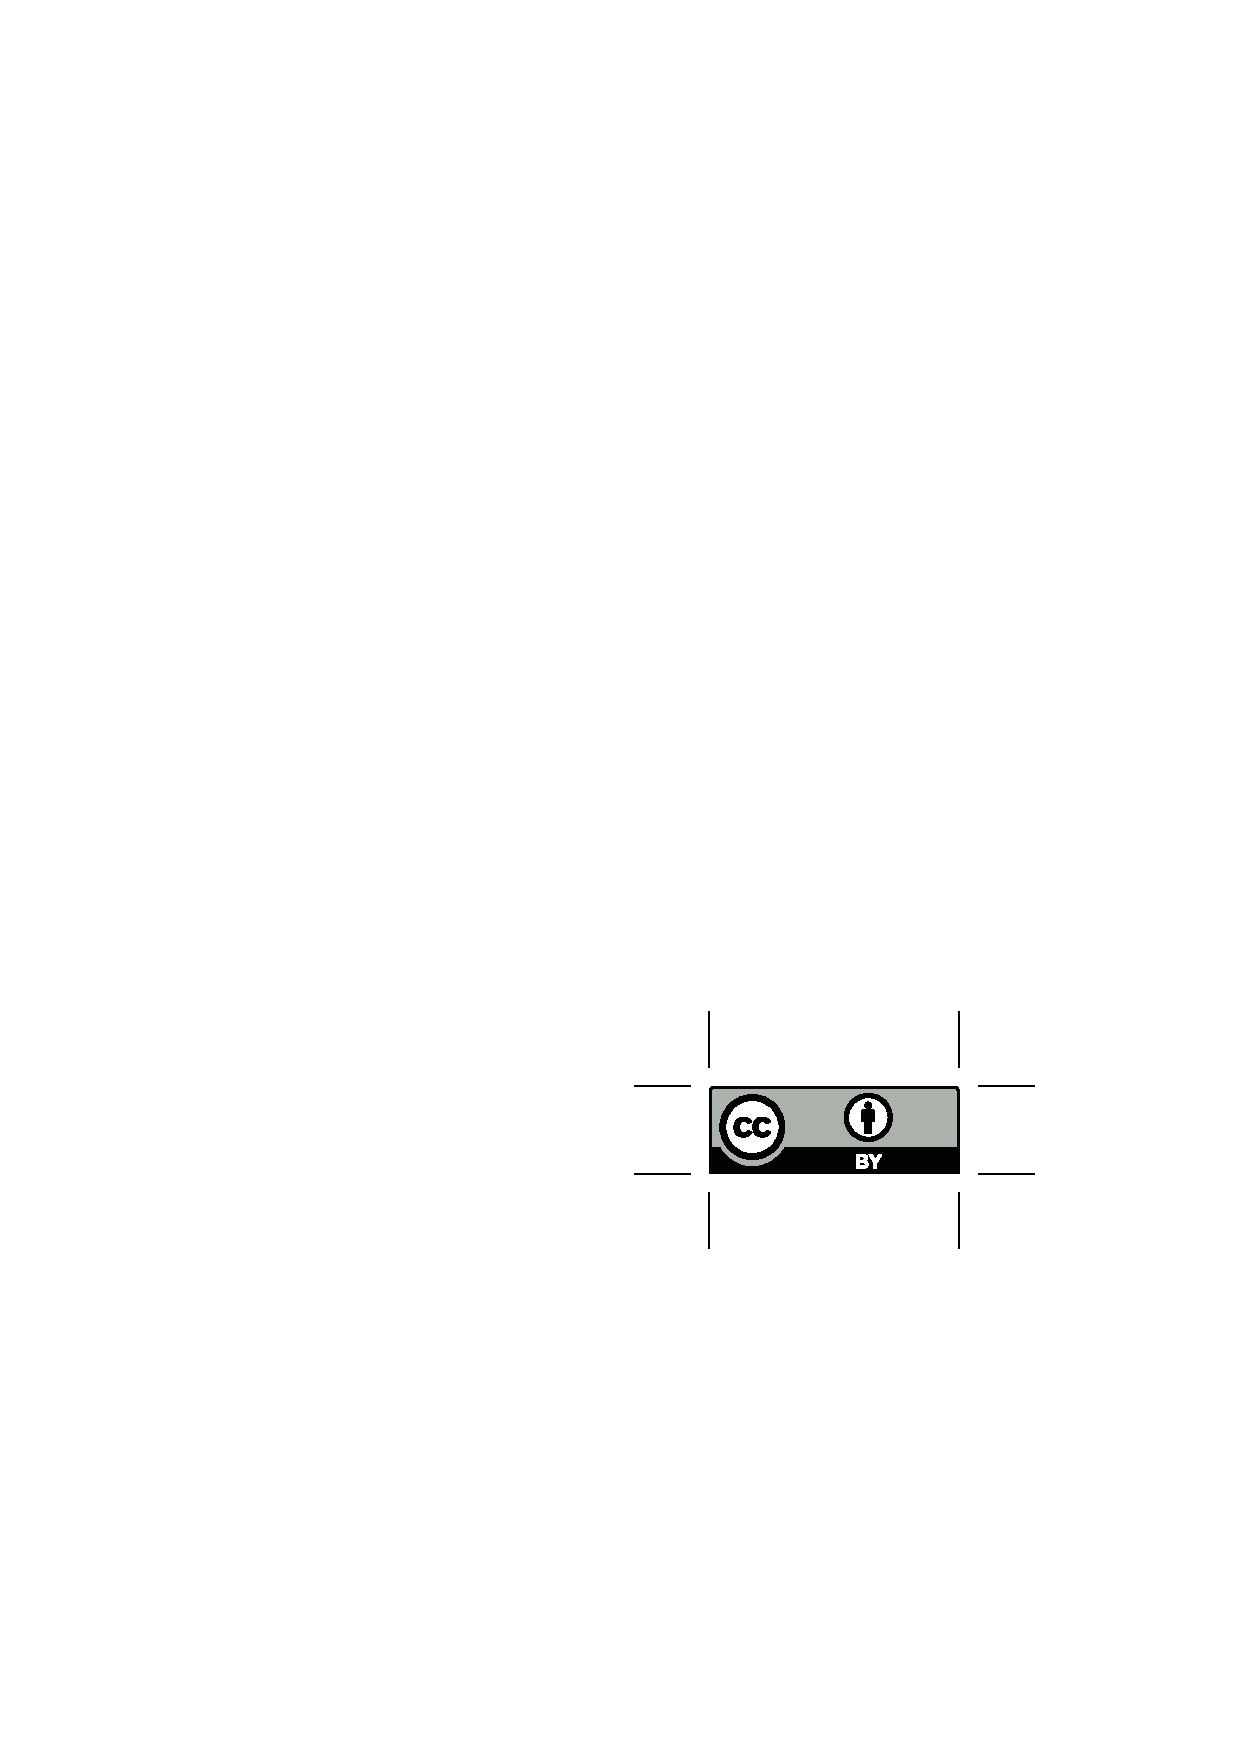
\includegraphics[width=2cm]{by}
\end{wrapfigure}

\noindent
``iPhone'', ``Alarm Clock'', ``Computer'' and ``Wireless'' symbols by The Noun Project, from The Noun Project collection.\\
``A graphic language for touch'', Timo Arnall.\\

\begin{wrapfigure}{l}{2.2cm} 
\centering

\includegraphics[width=2cm]{cc-zero}
\end{wrapfigure}

\noindent
``Desk Lamp'' symbol by Edward Boatman, ``Radio'' symbol by National Park Service, ``User'' symbol by Denis Chenu, ``Music'' symbol by Ryan Oksenhorn, from The Noun Project collection.\\


\noindent\myName: \textit{\myTitle,} \mySubtitle, %\myDegree, 
\textcopyright\ \myTime\\

\noindent
A catalogue record is available from the Eindhoven University of Technology Library.\\
ISBN: 978-90-386-3234-6\\

\noindent
Proefontwerp Technische Universiteit Eindhoven\\
Trefw.: Ontologies, Semantic Web, Software Architecture, Interaction Design


%\bigskip
%
%\noindent\spacedlowsmallcaps{Supervisors}: \\
%\myProf \\
%\myOtherProf \\ 
%\mySupervisor
%
%\medskip
%
%\noindent\spacedlowsmallcaps{Location}: \\
%\myLocation
%
%\medskip
%
%\noindent\spacedlowsmallcaps{Time Frame}: \\
%\myTime


\begin{titlepage}
	\begin{addmargin}[-1cm]{-3cm}
	\begin{center}
		
\newlength{\drop}

\drop=0.1\textheight 
\vspace*{\drop} 

{\LARGE \bfseries Ontologies for interaction}\\[1\baselineskip] 
{\Large\sffamily Enabling serendipitous interoperability in smart environments}\par 
\vfill
{\LARGE PROEFONTWERP}\par 
\vspace{\drop} 
{\large ter verkrijging van de graad van doctor aan de\\
Technische Universiteit Eindhoven, op gezag van de\\
rector magnificus, prof.dr.ir. C.J. van Duijn, voor een\\ 
commissie aangewezen door het College voor\\ 
Promoties in het openbaar te verdedigen\\
op dinsdag 9 oktober 2012 om 16.00 uur}\par
\vfill 
{\large door}\par
\vspace*{0.7\drop}
{\large Gerrit Niezen}\par 
\vspace*{0.7\drop} 
{\large geboren te Pretoria, Zuid-Afrika}\par
%\vspace*{0.5\drop}
\end{center}
\end{addmargin}
\end{titlepage}

\newpage
\thispagestyle{empty}
\begin{addmargin}[-1cm]{-3cm}
{\noindent De documentatie van het proefontwerp is goedgekeurd door de promotoren:}\\

{\noindent prof.dr.ir. L.M.G. Feijs}\\
en\\
prof.dr. P. Markopoulos\\

{\noindent Copromotor:}\\
dr. J. Hu PDEng MEng\\
\end{addmargin}

\cleardoublepage
%*******************************************************
% Acknowledgments
%*******************************************************
\pdfbookmark[1]{Acknowledgments}{acknowledgments}

\begin{flushright}{\slshape    
    We have seen that computer programming is an art, \\ 
    because it applies accumulated knowledge to the world, \\ 
    because it requires skill and ingenuity, and especially \\
    because it produces objects of beauty.} \\ \medskip
    --- {Donald E. Knuth}%\defcitealias{knuth:1974}\citetalias{knuth:1974} \citep{knuth:1974}
\end{flushright}



\bigskip

\begingroup
\let\clearpage\relax
\let\cleardoublepage\relax
\let\cleardoublepage\relax
\chapter*{Acknowledgments}
Put your acknowledgments here.

I would like to thank Aly Syed, Riccardo Trevisan, Sriram Srinivasan, Hans van Amstel, Stefan Rapp, Sachin Bhardwaj and Tanir Ozcelebi for their contributions to the smart home pilot.

Holger Knublauch and Scott Henninger from TopQuadrant

\bigskip

\noindent\emph{Regarding \mLyX}: The \mLyX\ port was intially done by 
\emph{Nicholas Mariette} in March 2009 and continued by 
\emph{Ivo Pletikosi\'c} in 2011. Thank you very much for your 
work and the contributions to the original style.


\endgroup




%\cleardoublepage
%*******************************************************
% Dedication
%*******************************************************
\thispagestyle{empty}
%\phantomsection 
\refstepcounter{dummy}
\pdfbookmark[1]{Dedication}{Dedication}

\vspace*{3cm}

\begin{center}
    \emph{Ohana} means family. \\
    Family means nobody gets left behind, or forgotten. \\ \medskip
    --- Lilo \& Stitch    
\end{center}

\medskip

\begin{center}
    Dedicated to the loving memory of Rudolf Miede. \\ \smallskip
    1939\,--\,2005
\end{center}
%\cleardoublepage\include{FrontBackmatter/Foreword}


\pagestyle{scrheadings}
\cleardoublepage
%*******************************************************
% Table of Contents
%*******************************************************
%\phantomsection
\refstepcounter{dummy}
\pdfbookmark[1]{\contentsname}{tableofcontents}
\setcounter{tocdepth}{2} % <-- 2 includes up to subsections in the ToC
\setcounter{secnumdepth}{3} % <-- 3 numbers up to subsubsections
\manualmark
\markboth{\spacedlowsmallcaps{\contentsname}}{\spacedlowsmallcaps{\contentsname}}
\tableofcontents 
\automark[section]{chapter}
\renewcommand{\chaptermark}[1]{\markboth{\spacedlowsmallcaps{#1}}{\spacedlowsmallcaps{#1}}}
\renewcommand{\sectionmark}[1]{\markright{\thesection\enspace\spacedlowsmallcaps{#1}}}
%*******************************************************
% List of Figures and of the Tables
%*******************************************************
\clearpage

\begingroup 
    \let\clearpage\relax
    \let\cleardoublepage\relax
    \let\cleardoublepage\relax
    %*******************************************************
    % List of Figures
    %*******************************************************    
    %\phantomsection 
    \refstepcounter{dummy}
    %\addcontentsline{toc}{chapter}{\listfigurename}
    \pdfbookmark[1]{\listfigurename}{lof}
    \listoffigures

    \vspace*{8ex}

    %*******************************************************
    % List of Tables
    %*******************************************************
    %\phantomsection 
    \refstepcounter{dummy}
    %\addcontentsline{toc}{chapter}{\listtablename}
    \pdfbookmark[1]{\listtablename}{lot}
    \listoftables
        
    \vspace*{8ex}
%   \newpage
    
    %*******************************************************
    % List of Listings
    %*******************************************************      
	  %\phantomsection 
    % \refstepcounter{dummy}
    % %\addcontentsline{toc}{chapter}{\lstlistlistingname}
    % \pdfbookmark[1]{\lstlistlistingname}{lol}
    % \lstlistoflistings 
    % 
    % \vspace*{8ex}
       
    %*******************************************************
    % Acronyms
    %*******************************************************
    %\phantomsection 
    \refstepcounter{dummy}
    \pdfbookmark[1]{Acronyms}{acronyms}
    \markboth{\spacedlowsmallcaps{Acronyms}}{\spacedlowsmallcaps{Acronyms}}
    \chapter*{Acronyms}
    \begin{acronym}[UML]
	\acro{SOFIA}{Smart Objects For Intelligent Applications}
	\acro{SIB}{Semantic Information Broker}
	\acro{KP}{Knowledge Processor}
    \acro{SUMO}{Suggested Upper Merged Ontology}
	\acro{BFO}{Basic Formal Ontology}
	\acro{DUL}{DOLCE+DnS UltraLight}
	\acro{DnS}{Descriptions and Situations}
	\acro{COMM}{Core Ontology Multimedia}
	\acro{OWL}{Web Ontology Language}
	\acro{DOLCE}{Descriptive Ontology for Linguistic and Cognitive Engineering}
	\acro{FOAF}{Friend-Of-A-Friend}
	\acro{OWA}{Open World Assumption}
	\acro{BDI}{Belief Desire Intention}
	\acro{ODP}{Ontology Design Patterns}
	\acro{CP}{Content ontology design Pattern}
	\acro{SPIN}{SPARQL Inferencing Notation}
	\acro{SWRL}{Semantic Web Rule Language}
	\acro{DC}{Dublin Core}
	\acro{RDF}{Resource Description Framework}
	\acro{URI}{Uniform Resource Identifier}
	\acro{URL}{Uniform Resource Locator}
	\acro{IoT}{Internet of Things}
	\acro{UPnP}{Universal Plug and Play}
	\acro{DCP}{Device Control Protocol}
	\acro{DLNA}{Digital Living Network Alliance}
	\acro{IP}{Internet Protocol}
	\acro{AV}{Audio/Video}
	\acro{EEG}{Electroencephalography}
	\acro{FFT}{Fast Fourier Transform}
	\acro{ANN}{Artificial Neural Network}
	\acro{REM}{Rapid Eye Movement}
	\acro{MOM}{Message-Oriented Middleware}
	\acro{JMS}{Java Message Service}
	\acro{AMQP}{Advanced Message Queuing Protocol}
	\acro{MSMQ}{Microsoft Message Queuing}
	\acro{STOMP}{Streaming Text Oriented Messaging Protocol}
	\acro{XMPP}{Extensible Messaging and Presence Protocol}
	\acro{IETF}{Internet Engineering Task Force}
	\acro{GUI}{Graphical User Interface}
	\acro{GAS}{Gadgetware Architectural Style}
	\acro{DAML}{DARPA Agent Markup Language}
	\acro{OIL}{Ontology Inference Layer}
	\acro{FSM}{Finite State Machine}
	\acro{XML}{Extensible Markup Language}
	\acro{GENA}{Generic Event Notification Architecture}
	\acro{CAMUS}{Context-Aware Middleware for Ubiquitous computing Systems}
	\acro{FIPA}{Foundation for Intelligent Physical Agents}
	\acro{UIMS}{User Interface Management System}
	\acro{UIRS}{User Interface Runtime System}
	\acro{MVC}{Model-View-Controller}
	\acro{MCRpd}{Model-Control-RepP-RepD}
	\acro{CLG}{Command Language Grammar}
	\acro{ASUR}{Adapter, System, User, Real object}
	\acro{SOUPA}{Standard Ontology for Ubiquitous and Pervasive Applications}
	\acro{CoBrA}{Context Broker Architecture}
	\acro{NFC}{Near Field Communication}
	\acro{UUID}{Universally unique identifier}
	\acro{SPARQL}{SPARQL Protocol and RDF Query Language}
	\acro{RFID}{Radio Frequency Identification}
	\acro{API}{Application Programming Interface}
	\acro{SQL}{Structured Query Language}
	\acro{PC/SC}{Personal Computer/Smart Card}
	\acro{ACS}{Advanced Card Systems}
	\acro{SSAP}{Smart Space Access Protocol}
	\acro{SAN}{System Architecture and Networking}
	\acro{QCR}{Qualified Cardinality Restriction}
	\acro{OSGi}{Open Services Gateway initiative}
	\acro{RL}{Rule Language}
	\acro{XSD}{XML Schema Definition}
	\acro{ANR}{Application Not Responding}
	\acro{CC/PP}{Composite Capabilities/Preferences Profile}
	\acro{UIML}{User Interface Markup Language}
	\acro{XIML}{Extensible Interface Markup Language}
	\acro{PUC}{Personal Universal Controller}
	\acro{INCITS/V2 URC}{International Committee for Information Technology Standards Universal Remote Console}
	\acro{RUI}{Remote User Interface}
	\acro{VNC}{Virtual Network Computing}
	\acro{RDP}{Remote Desktop Protocol}
	\acro{RFB}{Remote Framebuffer}
	\acro{UAProf}{User Agent Profile}
	\acro{DCS}{Distributed Communication Sphere}
	\acro{ASIN}{Amazon Standard Identification Number}
	\acro{NORA}{Non-Obvious Relationship Awareness}
	\acro{EO}{Event Ontology}
	\acro{LODE}{Linked Open Descriptions of Events}
	\acro{GoF}{Gang of Four}
	\acro{TUI}{Tangible User Interface}
	\acro{IOP}{Interoperability Platform}
	\acro{MQTT}{Message Queue Telemetry Transport}
	\acro{RIBS}{RDF Information Base System}
	\acro{CWA}{Closed World Assumption}
\end{acronym}


\endgroup

\cleardoublepage
%********************************************************************
% Mainmatter
%*******************************************************
\pagenumbering{arabic}
%\setcounter{page}{90}
% use \cleardoublepage here to avoid problems with pdfbookmark
\cleardoublepage
\ctparttext{You can put some informational part preamble text here. 
Illo principalmente su nos. Non message \emph{occidental} angloromanic
da. Debitas effortio simplificate sia se, auxiliar summarios da que,
se avantiate publicationes via. Pan in terra summarios, capital
interlingua se que. Al via multo esser specimen, campo responder que
da. Le usate medical addresses pro, europa origine sanctificate nos se.}
\part{Framing the problem and current state-of-the-art}
\chapter{Introduction}
\label{Introduction}

\begin{flushright}{\slshape    
The real problems going forward are not with any single device, \\
but in the potential complexity of the larger ecosystem of \\
technologies that we function in. [...] It's about the society \\
of appliances and how they work today which is the new frontier.} \\ \medskip
    --- Bill Buxton \cite{Buxton2010}
\end{flushright}

\marginpar{Parts of this chapter appear in \cite{Niezen2010} and \cite{Niezen2011}.}

%-- 20-liner
When trying to share music or photos between your mobile phone and that of a friend, making the connection between the two devices is not always straightforward. You need to select the appropriate communication technology and identify the target device from a list of possible options. Manufacturers often only allow sharing between devices that form part of their own ecosystem, where devices from other manufacturers may be incompatible with this ecosystem. In the future there could be hundreds of devices in your immediate surroundings, and these devices, created by different manufacturers, will need to work with another.

What if we want to share more than just media, or want to use one device to control another? As an example, imagine connecting a sleep monitor to the lamp on your bedside table, helping you to wake up at the right time in your sleep cycle. This thesis focuses on ways to create meaningful connections between devices, based on the functionality of the devices. We develop techniques for designers and developers to describe the capabilities of devices, such that the content and functionality can be shared with other devices. We also make use of different types of feedback to indicate what the possibilities for interaction are, as well as making the events that occur within this system of networked objects more transparent.

%---
\marginpar{Mark Weiser \cite{Weiser1991} coined the term ubiquitous computing, sometimes seen in its shortened form as ``ubicomp''.}
Key to realising the vision of ubiquitous computing \cite{Weiser1991} is ``serendipitous interoperability'', where devices which were not necessarily designed to work together should be able to discover each other's functionality and be able to make use of it \cite{Owl2004}. Future ubiquitous computing scenarios involve hundreds of devices, appearing and disappearing as their owners carry them from one room or building to another. Therefore, anticipating all the different types of devices and usage scenarios a priori is an unmanageable task. 

Next to serendipitous interoperability, another enabling strategy of ubiquitous computing is to make technologies --- as from a user's perspective they are still dealing with technologies --- disappear, and ``weave themselves into the fabric of everyday life until they are indistinguishable from it'' \cite{Weiser1991}. To reach this goal, self-configuration of the various devices and technologies in ubiquitous computing environments is essential. Whether automated and initiated by context-aware entities, or initiated by users by connecting the devices to one another, the actual configuration of the various components at a lower level should happen automatically.

\section{Background}

\subsection{Multi-device user interaction}

As computers disappear into the environment, we will need new kinds of human-computer interactions to deal with the peculiarities of these smart environments, which include invisible devices, implicit interaction, and distinguishing between physical and digital interactions \cite{Ye2007}. In the conventional \ac{GUI} genre, designers have typically developed prepackaged solutions for a predetermined interaction space, forcing users to adapt to their specific interaction protocols and sequences. In ubiquitous computing environments, the interaction space is unpredictable and emerges opportunistically \cite{Coutaz2005a}. There is the risk of creating a mismatch between the system's model of interaction and the user's mental model of the system. In these conditions, new interaction techniques must be devised to help users to construct helpful mental models, in order to minimise system and user model mismatches. These interaction techniques should also match the context of use that is dynamic and unpredictable. 

% A related issue is how ubiquitous computing differs from the sequential nature of traditional \ac{GUI} interaction. The single point of control that is usually available in such interfaces naturally leads to a sequential organisation of interaction. One step inevitably leads to the next; as an example, consider a dialog box that refuses to let you do anything else until you click either \texttt{OK} or \texttt{Cancel}. When we interact with a smart environment, it is not only the parallel nature of the interaction with the physical world that is different, but also \emph{the many different ways that we might map our tasks onto the features of the environment} \cite{Dourish2004}. Another difference is that these are not necessarily single-user interactions, but multiple users interacting in the same smart environment at the same time.

If we are able connect smart devices to one another effortlessly, it becomes possible to support high-level services, that would usually involve multiple steps on multiple devices \cite{Rich2009}. From a user's point of view, streaming music from a mobile device to a home entertainment system is a single high-level task. In practice there are multiple steps involved, and if the devices involved are from different manufacturers, the user needs to learn the operational details of each device interface in order to perform the task. From a technical perspective \ac{UPnP} with its device control protocols \cite{uPnPDCP} is not considered an adequate solution, because it only provides static device description documents and covers a very limited number of use cases. %From a user perspective \ac{UPnP}

At home the average person interacts with many devices during the course of a day. Sometimes these devices are used by more than one person, or one device may be used as an interface to another. As these devices are manufactured by different companies, there exist many different user interfaces that must be studied before they can be used. There might even be more than one way to interact with a single device. For example, to turn down the volume on a home entertainment system, either a remote control or a volume dial on the entertainment system itself may be used. It is expected that in future, more generic tools will be used to discover, configure, connect and control all the devices in the environment \cite{Newman2002}. 

\subsection{Configuring connections between devices}

In a world where we are potentially surrounded by a multitude of devices, allowing for the arbitrary ad hoc interconnection of devices, and the sharing of information between these devices, is difficult. It is unreasonable to expect that a device will have prior knowledge of all the different ways it can interact with surrounding devices. The number of possibilities are too large, and anticipating the potential number of interactions is infeasible. If we could add meaning to the interactions and interconnections in such a way that it is machine-readable, semantic web technologies could be used to infer additional properties about the existing entities. This could fill the gaps between that which is described in terms of device capabilities, and that which is possible in terms of combined functionality. The user is still the final arbiter in deciding what the device does, but the device should be capable of communicating the possibilities based on what was inferred from its environment. 

Besides the technological challenges, there also lies a challenge ahead for designing user interactions with these ecosystems of interconnected devices. When moving away from interaction with a single device towards interactions with systems of devices, designers need to communicate the relationships between the devices, and the larger system they are part of. Additionally, designers need to find ways to communicate the action possibilities of new, ``emergent functionalities'' \cite{Frens2009}, that emerge when devices are being interconnected. 

An important problem that arises when designing for these systems of interactive objects is their highly interactive and dynamic nature \cite{Frens2009}. The inherent ever-changing nature of these systems and the severely limited overview of the ecosystem in its entirety is one of the most important challenges a designer faces when designing for such systems. Additionally, such a system comprises many different ``nodes'' that the designer, at the time of designing has no control over. Yet, when designing and adding new nodes to the system, making them interoperable is crucial for success. 

According to Newman et al. \cite{Newman2002}, the following should be communicated to a user attempting to interact with and establish connections between devices:
\begin{itemize}
\item What devices and services are available
\item Capabilities of the devices and services
\item Relationships between each another and the environment
\item Predictions of likely outcomes from interaction
\end{itemize}

The information presented to the user should be filtered dynamically, based on the user's context. This context includes for example the user's location, interaction history, and current tasks. A smart object is able to sense the context of its surroundings, make use of this context and other information to proactively interact with users and other smart objects, and self-organise into groups with other devices \cite{Sabou2010}. This context information should be represented in such a way that is understood by all the entities in the system. 

%When people think of systems that try to infer what they are doing from their actions, they inevitably think of Clippy, Microsoft's Office Assistant, that tried to offer help based on a user's actions.

The background described in this section provides for interesting design challenges and research questions that can be asked. In the following section we will first discuss the context of the work described in this thesis, followed by the research questions that were addressed.







\section{Context of the work and research questions}

The work described in this thesis was completed as part of a European research project called \ac{SOFIA}\footnote{http://www.sofia-project.eu/}. Some of the design choices were guided by collaboration with partners in the \ac{SOFIA} project. We worked with the project partners to elicit requirements and expose ourselves to other application areas, in order to gain a more holistic view of the problem.


\subsection{The SOFIA project}\label{sofia}

\ac{SOFIA} is an European research project within the ARTEMIS framework that attempts to make information in the physical world available for smart services --- connecting the physical world with the information world. The goal is to enable cross-industry interoperability and to create new user interaction and interface concepts, to enable users to benefit from smart environments. The centre of the software platform developed within \ac{SOFIA} is a common, semantic-oriented store of information and device capabilities called a \ac{SIB}. Various virtual and physical smart objects, termed \acp{KP}, interact with one another through the \ac{SIB}. The goal is that devices will be able to interact on a semantic level, utilising (potentially different) existing underlying services.

%thimbleby
\label{sofiatuple}
The \ac{SOFIA} software platform is based on the ideas of space-based computing, where near linear scalability can be achieved using the tuple space paradigm. A tuple space is a repository of tuples, where a tuple is an ordered list of elements. Tuple-based computing has been introduced in parallel programming languages to implement communication between parallel processes \cite{Fensel2004}. Producers send their data as tuples to the space, and consumers read tuples from the space. This is also known as the blackboard metaphor.

Our focus within the \ac{SOFIA} project was on the user interaction aspects of devices in the smart home environment. While most of the examples in this thesis are specific to the smart home environment, the concepts are also applicable in the wider context of ubiquitous computing, for example the smart city or smart personal spaces. %We now look at the context of the work in terms of two complementary visions described in the literature: Ubiquitous computing and ambient intelligence.
We now consider the context of the work in terms of the vision of ubiquitous computing.

\subsection{Ubiquitous computing}

%Mark Weiser \cite{Weiser1991} coined the term ubiquitous computing, sometimes seen in its shortened form as ``ubicomp''. 
The vision of ubiquitous computing describes a future where electronic devices are so ubiquitous that their presence is not noticed anymore. As described earlier in this chapter, we consider the enabling technological strategies of ubiquitous computing to be serendipitous interoperability and making technologies disappear.

Chalmer and MacColl \cite{Chalmers2003} questioned the more recent assumption in ubiquitous computing research that devices should disappear into the environment, reiterating Weiser's original vision that tools for interaction should be ``literally visible, effectively invisible''. There is a difference between physical and cognitive disappearance. Where the term physical disappearance describes the trend of devices to be embedded into the environment, cognitive disappearance means that the user does not distinguish between the computer and the artefact anymore, but focuses on the function of the artefact. Devices should retain their unique characteristics, even when placed within systems of devices. Users are influenced by how they perceive devices, and we have to accept that the devices themselves are part of the user's context.

Ubiquitous computing products are a combination of hardware, software and services. It is not clear what kind of skills are required to design for this kind of environment \cite{Kuniavsky}. There is, however, a need for interaction designers and software developers to have a common vocabulary and framework when cooperating to create these products. This thesis attempts to move this idea forward, by defining common concepts that are prevalent in most ubiquitous computing environments, and establishing a framework that can be used by both designers and developers alike.

% \subsection{Ambient Intelligence}
% The Ambient Intelligence paradigm differs from that of Ubiquitous Computing in that it tries to create environments that are sensitive  to and responsive to the presence of people \cite{Aarts2004}. Devices disappear into the environment, necessitating virtual devices to support user interaction. It is expected that the devices adapt to to and even anticipate the user's needs. While our work is in principle closer to the vision of ubiquitous computing than ambient intelligence, there are some important aspects of ambient intelligence that need to be considered.
% 
% % Start of SISS2010 Conclusion
% 
% Marzano and Aarts \cite{Aarts2004} formulated the following five key technology features to define the notion of ambient intelligence:
% 
% \begin{itemize}
% \item Embedded - many networked devices are integrated into the environment.
% \item Context aware - the system can recognise the user and his/her situational context.
% \item Personalised - the system can tailor itself to meet the user's needs.
% \item Adaptive - it can change in response to the user.
% \item Anticipatory - the system anticipates the user's desires without conscious mediation.
% \end{itemize}
% 
% Personalisation refers to system adjustments made on short time scale, for example installing personalised settings. Adaptation involves adjustments made by monitoring the user over a longer period of time. For anticipation, the system needs to be able to detect behavioural patterns that occur over a very long period of time.
% 
% %We consider context awareness to be one of the most important features of a smart environment, especially when we consider a user's interaction with the smart space. Considering the parallel nature of our interaction with the physical world, any smart space will require context to help it make sense of the many different ways in which users map their tasks onto the environment.
% 
% Where the system tries to predict what the user is trying to accomplish, by being adaptive and anticipatory, we need to identify ways to give the users appropriate means to express themselves. The possibilities, available services and information that exist in the smart environment need to be communicated in a meaningful way. Only if this is done correctly will users be able to build helpful mental models of the functionality the environment has to offer, set goals and make plans on how to act. By developing novel and meaningful interaction devices, the user can then perform the necessary actions and the system can in turn try to understand the user's goals and make the match to its internal models. We see a vital role here for the theory of \emph{product semantics} \cite{Feijs2009}, the study of how artefacts acquire their meaning, where we can use its theories to define common concepts and semantics.
% 
% The ambient intelligence paradigm shows the importance of feedback in adaptive and anticipatory environments. In the thesis we describe the different kinds of feedback and feedforward that are applicable to these environments, as well as how it was implemented in a use case scenario. 


\subsection{Affordances}

In their article ``At Home with Ubiquitous Computing: Seven Challenges'', Edwards and Grinter \cite{Edwards2001} describes a scenario where a couple come downstairs in the morning intent on listening to the radio, and realise that there is no sound coming from their speakers. It turns out that the neighbours bought a new set of Bluetooth-enabled speakers which, when installed, associated themselves with the nearest sound source -- the couple's Bluetooth-enabled stereo.

The wireless nature of the speakers does away with the traditional affordances making connections between the speakers and the stereo. These affordances are explicit when physical wires are used - the connections can be observed and the range of connectivity is clear. Edwards and Grinter state that the design challenge is to provide \emph{affordances}\label{Affordances} that help users understand the technology, allowing them to control, use and debug technologies that interact with one another in the environment. 

Norman \cite{Norman1999} defined affordances as the perceived and actual properties of an object, primarily those properties that determine how an object should be used. The set of action possibilities of an object is based on its appearance, but also on the actual interaction with that object. An affordance is a relationship between an object and the person acting on the object, such that the same object might have different affordances for different individuals. The term was originally created by the psychologist J.J. Gibson to describe human perception \cite{Gibson1977}, but was extended by Norman for its application to design.

%Complex interactions between numerous interconnected computers and devices, where functionality is distributed across several devices that are spontaneously discovered and used, need to be managed \cite{Lee2006}.

% Interaction metaphors \cite{Kuniavsky} provide handles to these invisible technologies, where the metaphors are used to establish ideas about the meaning of physical affordances and potential ways to use these devices. For example, a Nintendo WiiMote is waved around much like a magic wand, so we can use ``an enchanted object'' as the interaction metaphor for the device.

\subsection{Ontologies}

The current state of ubiquitous computing is similar to that of desktop computing in the 1970s, where there is a whole range of new technologies without metaphors to communicate how they operate. The question then becomes how we then can model a device, not only in terms of its technical characteristics or capabilities, but also in terms of user interaction and feedback, where metaphors, functionality and affordances play an important role.

One possible solution to modelling devices is to make use of ontologies, a concept in computer science most often associated with the Semantic Web \cite{Berners-Lee2001}. Ontologies are formal representations of knowledge, consisting of various entities that are related to one another. They provide a shared vocabulary, which makes it easier to publish and share data. Ontologies allow us to model a domain in terms of its concepts, and the relationships between these concepts. They are also both machine-readable and human-understandable.

Ontologies are well suited to environments with a large number of devices. They have been designed to work at Web scale, they enable heterogeneous data sources to interoperate with one another, and they are based on technology standards which allow for easy and large scale adoption \cite{Sabou2010}.
 
Ontologies lend themselves well for describing the characteristics of devices, the means to access such devices, and other technical constraints and requirements that affect incorporating a device into a smart environment \cite{Owl2004}. Using an ontology also simplifies the process of integrating different device capability descriptions, as a semantic inferencing engine can be used to infer relationships between the concepts in the descriptions.


\subsection{Research questions}
\label{ResearchQuestions}
The hypothesis of this thesis is that \emph{user interaction in a smart environment can be better supported by ontological models than with existing device and service descriptions} (e.g. descriptions stored in relational databases). These ontological models define a semantic mapping between the user's behaviour and the available resources in the environment.

%Should be measurable, specify what is compared and what is being verified. Relate to existing body of knowledge. Research question should be stated in observable, measurable terms

\marginpar{``The greatest challenge to any thinker is stating the problem in a way that will allow a solution.'' -- Bertrand Russell}

The thesis aims to answer a number of research questions. In the previous section, ontologies were offered as a potential solution to solving the interoperability problem in ubiquitous environments. They are also well suited to describing user interaction in such an environment. This leads us to the first question:

\begin{question}
How can we use an ontology to model user interaction and devices in a smart environment consisting of multiple devices and multiple interactions? 
\end{question}

%thimbleby
Related work on ontologies \cite{Chen2004,Ranganathan2004,Ngo2004}, described in more detail in the next chapter, focused mainly on modelling context and basic device properties. The ontologies created as part of the work described in this thesis is not only an attempt to model device capabilities in more detail, but to our knowledge is also the first attempt to model user interaction in a smart environment. 

%This question is addressed in Chapters \ref{DeviceCapabilityModelling}, \ref{EventModelling} and \ref{OntologyEngineering}. %How can interaction events be modeled, represented and reasoned about using a ontology language?

% TODO Discuss http://en.wikipedia.org/wiki/Publish/subscribe, or change to blackboard pattern
\label{blackboard}
In the \ac{SOFIA} project, \acp{KP} communicate with a message broker using the blackboard architectural pattern, where the message broker contains a common knowledge base. This knowledge base, consisting of a triple store and an ontology, is used to share information between the various knowledge sources.

\begin{question}
How suitable is the blackboard architectural pattern for handling ontology-based ubiquitous computing environments? 
\end{question}

%thimbleby
The advantage of a blackboard architecture is that it decouples reference, time and space \cite{Fensel2004}. Communicating processes do not need to explicitly know each other, i.e. reference-wise they are decoupled. The blackboard guarantees persistent storage, such that communication can be asynchronous and decoupled time-wise. As long as they have access to the same blackboard, processes can run anywhere, decoupling them space-wise. We can compare the performance of our implementation against related work on blackboard-based architectures for ubiquitous computing environments \cite{Winograd2005,Etelapera2011}. 

%Chapter \ref{SoftwareArchitecture} seeks to answer this question.

If we make use of a triple store and ontology, a semantic reasoning engine is required to perform inferencing on the knowledge base of asserted triples. If triples are frequently inserted and removed, the time required for inferencing could have an adverse effect on the responsiveness of the user interface.  

\begin{question}
How responsive is a networked user interface that is implemented on top of a system architecture with a semantic reasoning engine? 
\end{question}

%This question is addressed in Chapter \ref{Evaluation}.

Some work has been done to measure the usability of \acp{API} for developers \cite{Robillard2009}. However, we do not have a way to evaluate the usability of software frameworks and ontologies for ubiquitous computing environments from a developer point-of-view. 

\begin{question}
How can we measure the usability of ontologies and software frameworks for developers of ubiquitous computing environments? 
\end{question}
%This is explored further in Chapter \ref{Evaluation}.

Feedback is required to help the user make sense of what is happening in the environment. When we consider multiple interconnected smart objects, feedback and feedforward gets spatially distributed. 

\begin{question}
How should feedback be provided in a networked user interface consisting of multiple connected devices? 
\end{question}
%A possible solution to this problem is presented in Chapter \ref{DesignIteration3}.

%How can description logic be applied to the modelling of smart environments?

% How should the capabilities of devices in the environment be modelled in order to perform semantic mapping?
	
%How can we use semantic reasoning to infer user intention in a smart environment?

%After making inferences about the user, how should a user-adaptive system respond?

%What emergent knowledge is created through ad-hoc interactions between connected devices?

%Why is an ontological approach better than existing approaches, e.g. relational database?

%\end{itemize}

%- Describe devices based on their capabilities/attributes, and use reasoner to infer connection possibilities.
%- Multi-device user interaction
%- Abstracting low-level interaction events into higher-level actions/goals/tasks
%- Functional coupling between mobile devices
%-  
%- Information filtering based on context and current goals
%- Publish/Subscribe messaging paradigm
% - Systems that obtain user input through sensing user action, rather than through standard input devices such as the keyboard, mouse or stylus.
%- Does not cover graphical user interfaces, but interaction events

%Building a model of the user's interaction with the smart space allows us to establish a semantic mapping between user behaviour and the environment. 
%Ontological modelling may be used to create an interaction model of a user's interaction with the smart space, including the user's profile, preferences, goals and intentions. We may use the interaction model to map the user's tasks or goals onto the devices available in the smart space.  Devices should focus on supporting people's stated intentions, desires and needs, rather than trying to anticipate them \cite{Kuniavsky}.

\section{Methodology}

\begin{figure}
\centering
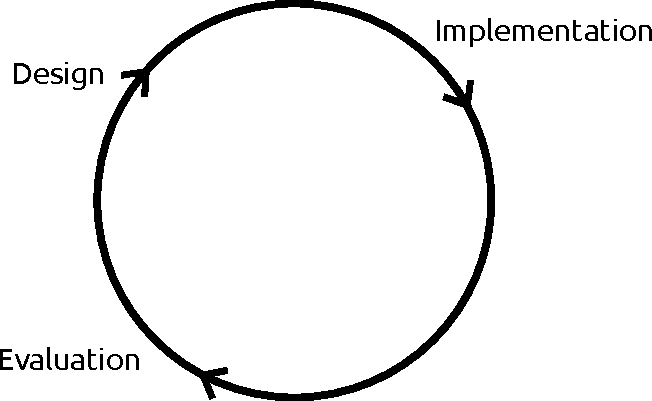
\includegraphics[width=250px]{methodology}
\caption{Iterative design methodology}
\label{methodology}
\end{figure}

%there should be a separate section "approach" or "methodology", to present the methods and the process of the investigation, and in answering the research questions.

An iterative design methodology \cite{Larman2003} was followed for the work described in this thesis. This cyclic process, shown Figure \ref{methodology}, consists of three steps -- design, implementation and evaluation -- where the results of the previous iteration are used as input for the next iteration. Iterative design is commonly used in the development of human-computer interfaces, but applies to many fields, including industrial design and software engineering.

%thimbleby
The research described in this thesis can be aligned to the triangulation framework of Mackay and Fayard \cite{Mackay1997}, as shown in Figure \ref{roadmap}. This framework integrates scientific and design models, by combining the deductive and inductive approaches with the design approach. With the deductive approach, research originates from theory, whereas with the inductive approach the research originates from observations. With the design approach, designers and engineers use guidelines and requirements as input to iterative prototypes used to construct a final product.

The framework shows how the design iterations are related to the constructed theories and models, as well as the evaluations and observations. The framework provides a roadmap of the work described in this thesis, where the relevant chapters are indicated in the figure.
  
\begin{figure}
\centerline{
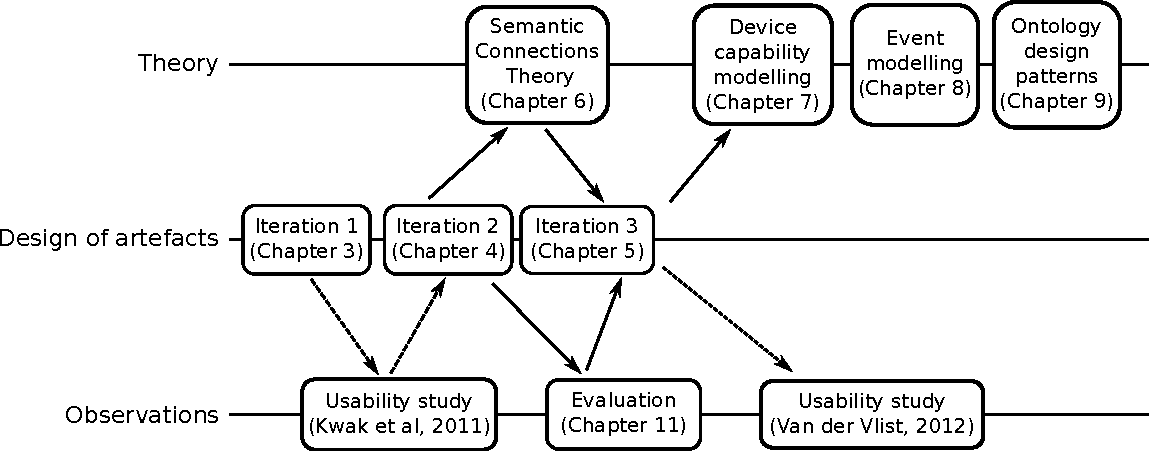
\includegraphics[width=450px]{Roadmap}}
\caption{The research approach used in the thesis}
\label{roadmap}
\end{figure}


\section{Outline of the thesis}

In the remainder of Part A the related work, including relevant research projects, is discussed. Existing state-of-the-art ontologies for ubiquitous computing environments and context-aware systems are described, followed by a description of the various interaction models, task models and semantic models that were used as basis for our own interaction model. 

An iterative approach was followed during the design process. Part B describes the three design iterations, detailing the requirements, design, implementation and evaluation processes. A theory of semantic connections is introduced, based on the output from the design iterations, that focuses on the meaning of the connections between the different entities in a smart environment. It is intended to enable interaction designers and developers to create interoperable smart objects, providing them with a common vocabulary and framework. The \ac{SOFIA} software architecture was taken as a departure point during each of the design iterations described in Part B. The various extensions and changes to the reference architecture are described in more detail in each design iteration description. 

From the work done, concepts and techniques that can be applied to ubiquitous computing in general were discovered. These concepts and techniques were extracted from the design iterations and are discussed in more detail in Part C, to exist independently of the design iterations. Our approach to modelling the interaction capabilities of smart objects is described, which builds on earlier ontologies for context-aware systems. Another contribution of this thesis is in the way interaction events are modelled, utilising existing event modelling techniques to describe user interaction in smart environments. Ontology design patterns that were identified and used during the course of the design are documented. A proposed software architecture to be used in future ubiquitous computing scenarios, based on the work done within \ac{SOFIA}, is described. This is followed by an evaluation of the work, which includes a performance evaluation and usability analysis. 



%In this thesis, the various models and technologies that may be combined to allow for semantic interaction in smart environments are investigated. 
%  We also consider whether the blackboard architectural pattern, used by SOFIA to enable a smart space-based computing environment, may be combined with runtime task models and the Belief-Desire-Intention (BDI) model, to result in a usable software architecture for pervasive computing.




\chapter{Related Work}

\begin{flushright}{\slshape
The old computing was about what computers could do; the new \\
computing is about what users can do. Successful technologies\\
are those that are in harmony with users' needs. They must \\
support relationships and activities that enrich the users' \\
experiences. } \\ \medskip
	    --- Ben Shneiderman
	\end{flushright}

In this chapter we describe related work. The work can be related in several ways, depending on which aspect of the work is considered. Therefore the chapter is subdivided into five sections, each devoted to one aspect. These are related projects and frameworks (Section \ref{RelatedProjects}), ubicomp ontologies (Section \ref{UbicompOntologies}), user interface software architectures (Section \ref{uisa}), modelling input devices (Sections \ref{interactionTasks}) and semantic models (Section \ref{SemanticModels}).


\section{Related projects and frameworks}
\label{RelatedProjects}
% Possible TODO Amigo, Embassi
% 
% \subsection{Amigo}
% 
% The Amigo project\footnote{http://www.hitech-projects.com/euprojects/amigo/} is a European project that ran from 2005 to 2008. 

In the field of ubiquitous computing there are a substantial number of past and current projects and relevant software frameworks that exist, most of them in the area of context-aware computing. In the following sections we will focus on those projects that are the closest in scope to the issues that are addressed by the work described in this thesis:

\begin{itemize}
	\item Serendipitous interoperability, as addressed by the \emph{recombinant computing} approach of the SpeakEasy project
	\item Sharing information between devices, as addressed by the Event\-Heap shared event system and its \emph{tuple space protocol}
	\item Using one device to control another, as addressed by the \emph{opportunistic assemblies} of the the XWeb architecture
	\item Multi-device user interaction, as addressed by the \emph{Media Cubes} of the AutoHAN project
	\item Configuring connections between devices, as addressed by the \emph{plug-synapse model} of the e-Gadgets project
\end{itemize}



\subsection{SpeakEasy (circa 2000-2003)}

We cannot expect all devices to have a priori knowledge of all the other devices they might possibly be connected to. We can, however, expect users to have knowledge about the devices they might encounter in their environment. Even if my smart phone does not know how to communicate with a specific printer, the software infrastructure could provide the necessary technical building blocks to allow them to communicate. The user understands what a printer does and makes the decision to connect the smart phone to the printer, as well as what to print.

% Begin TiiS
% (this is in introduction)
% According to Newman et al. \cite{Newman2002}, the following should be communicated to the user:
% \begin{itemize}
% \item What devices and services are available
% \item Capabilities of the devices and services
% \item Relationships between each another and the environment
% \item Predictions of likely outcomes from interaction
% \end{itemize}

This line of thinking was a starting point for Newman et al \cite{Newman2002}, who developed an approach which they named \emph{recombinant computing}, used in the SpeakEasy project at Xerox PARC. With this approach components are designed with the thought that they may be used in multiple ways, under different circumstances and for different purposes. Components expose \emph{recombinant interfaces} that are simple, domain-independent programmatic interfaces governing how components can interoperate with one another.
% End TiiS

\label{InformationFiltering} % this part on information filtering was on Notational Velocity
The SpeakEasy project focused on what users might be trying to accomplish in a specific situation when connecting entities to one another. Possible examples include connecting devices in order to give a presentation, or in order to send contact information. They created templates of common tasks that contained a partially specified set of connections and entities, which could be fully specified and instantiated by users at run-time. An instantiated template was then added to a list of current tasks. It was noted that templates impose a layer of semantics on top of the raw infrastructure. Templates assisted users by constraining the available component choices to only those that were appropriate for the task at hand. For example, a template could be partially specified as

\begin{itemize}
	\item Task name: Give a presentation
	\item Connection: File -> Projector
	\item File name: Choose..
	\item Projector: Choose..
\end{itemize}

where the user can then specify the name of the file, for example a Powerpoint presentation, as well as the projector in the room from a list of possibilities.

The SpeakEasy environment consisted of a web application that allows users to browse for components, which can be viewed and organised in different ways, for example grouped by location or owner.\marginpar{The e-Gadgets project in Section \ref{egadgets} also made use of a web application to configure components.} The work described in this thesis takes a different approach to configuring components, by using tangible interaction techniques instead of \ac{GUI}-based interaction.

What can be learned from the SpeakEasy project is the importance of describing the interfaces of components, such that they can be combined with other components. These interface descriptions help to enable serendipitous interoperability, and are described in more detail in Chapter \ref{DeviceCapabilityModelling}. 


\subsection{EventHeap (circa 2000-2005)}

Stanford University's shared event system, called the EventHeap, provides a base set of capabilities that link devices in a room \cite{Winograd2005}. It allows users to move data and applications between areas, for example redirecting a pointer from one device to another. One of these devices, the DynaWall, is a wall-size touch-sensitive interactive display. Gesture-based interaction facilitates moving information objects from the wall from one side to another, by throwing and shuffling visual objects with different accelerations and sounds.

During the development of their system, they identified the following design guidelines:

\begin{itemize}
	\item Heterogeneity - Devices must be able to interoperate in spite of heterogeneity in software. Interfaces must be customised to work smoothly on different-sized displays with different input/output modalities.
	\item Dynamism - A software framework must handle applications and devices joining and leaving, while minimising the impact on other entities in the space.
	\item Robustness - Users will treat the devices in interactive workspaces as appliances that should not fail in inexplicable ways. Devices must provide for quick recovery.
	\item Interaction techniques - A long, large wall needs an interaction technique suited to its size and location (such as DynaWall's throwing and shuffling technique).\marginpar{We explored similar interaction techniques during the development of the Spotlight Navigation device, see Section \ref{SpotlightNavigation} and \cite{Rapp2010}.}
\end{itemize}

A tuple space is a repository of tuples, where a tuple is an ordered list of elements. Devices in EventHeap use a \emph{tuple space protocol} to communicate with one another, where particular tuples have meaning to certain parties \cite{Edwards2001}. This semantic agreement between parties is implemented by the developer, for example a tuple representing a request to scan an image.

The iStuff toolkit \cite{Ballagas2003} was developed within Stanford to explore post-\ac{GUI} interaction techniques, and makes use of the EventHeap system. The iStuff toolkit allows users to map wireless input devices like buttons, sliders, wands, speakers and microphones to different applications running on devices like the DynaWall.

% from TiiS paper

Patch Panel \cite{Ballagas2004} is a mechanism in the iStuff toolkit that tries to solve incremental integration, the problem of integrating new devices and applications that may not have a priori knowledge of each others existence or function. Patch Panel uses an approach called intermediation, with a decoupled communication model (such as publish/subscribe) for inter-component communication. \marginpar{A similar decoupled model was used for the work described in this thesis.} Patch Panel uses a set of mappings between triggers and output events to enable intermediation. These mappings are defined using the Patch Panel Manager \ac{GUI} or \ac{FSM}-based scripting language, and users configure connections using a web-based configuration wizard.

%They noted that SpeakEasy allows for direct user intervention via \acp{GUI}, but does not support automated connections free of user intervention, for example data from presence sensors that may be used to turn on the lights. 

% end TiiS

Existing toolkits like iStuff do not provide support for the association of high-level semantics to physical objects \cite{Shaer2004}. While our approach to sharing information between devices is similar to that of EventHeap and Patch Panel, it differs in in the following ways:

\begin{itemize}
    \item We use ontologies describe device capabilities and interaction events
    \item We use semantic reasoning to resolve semantic mismatches between device descriptions
    \item Tangible interaction is used instead of \ac{GUI}-based interaction to configure connections
\end{itemize}


\subsection{The XWeb architecture (circa 2001-2003)}
The goal of the XWeb architecture is to allow for \emph{opportunistic assemblies} of interactive resources in order to accomplish a particular task. Olsen et al \cite{Olsen2001} recognised that both an interactive model for acquiring and using the interaction resources, as well as an underlying infrastructure is needed. In their model, each interaction resource resolves user intent independently, instead of merging inputs from a variety of modalities.

A client-server architecture was used to create the infrastructure, with \ac{XML} objects used to model resources and services. Tasks were defined using a two-part \ac{URL} in the form \texttt{dataReference\-::viewReference}, where the \emph{view} is an abstract definition of a particular interaction. These views are defined as a tree of \emph{interactors}, where the data and the view of the current task as well as the path of the interactor is used to characterise the current state of the device.

XWeb uses a subscribe mechanism to allow multiple clients to share their information, where the devices themselves are not aware of each other but can still be integrated into the same task. The problem that is addressed is that the different devices can be connected without requiring a lot of configuration effort from the user.

Pierce and Mahaney \cite{Pierce2003} extended the XWeb approach to opportunistic assemblies with \emph{opportunistic annexing}, which is is the process of temporarily attaching one or more resources, like a speaker or a keyboard, to a device in order to enhance its capabilities. Opportunistic annexing differs from the other approaches in this section in that it extends the existing capabilities of devices, instead of assembling heterogeneous devices into a larger, aggregate device. %A higher-level description of user's actions, instead of raw input events, reduces the communication load and the amount of raw input events that need to be understood by the device itself. 


% \begin{table}
%     \myfloatalign
%   \begin{tabularx}{\textwidth}{Xll} 
% 	\toprule
%     \tableheadline{Name} & \tableheadline{Scale} & \tableheadline{Examples} \\ 
%     \midrule
% 	Covert & 1 cm & Watch, RFID badge, Bluetooth headset \\ %, iPod Shuffle
% 	Mobile	& 10 cm	& Laptop, camera, mobile phone \\ % e-book reader, 
% 	Personal & 1 m & ATM, desktop computer, automobile \\ %Microsoft Kinect, 
% 	Environmental &	10 m &	Television, Public display, Nintendo Wii \\
% 	Architectural & 100 m & Media facade, Arena scoreboard\\ %, Interactive art installation \\
% 	Urban & 1 km & Temporary giant ubicomp experiences \\
% 	
%     \bottomrule
%   \end{tabularx}
%   \caption{Kuniavsky's Scales of Ubicomp Device Design}
%   \label{MultiScale}
% \end{table}

%Opportunistic annexing allows interaction at one scale to be controlled by a device at a different scale. Kuniavsky \cite{Kuniavsky} defined the scales of ubicomp device design shown in Table \ref{MultiScale}. The name of each scale is meant to convey the size of devices at that scale, similar to Greenfield's \cite{Greenfield2006} description of \emph{everyware}, acting ``... at the scale of the body, [...] the room, [...] the building, [...] the street, and of public space in general''.

Pierce and Mahaney expect that the primary benefit of annexing input resources will be faster input rates. This means that the actual annexing action should be faster than the time required to perform the action. For example, if a user will save 5 seconds by typing a note on a keyboard rather than on a mobile device, annexing the keyboard to the mobile device should take less than 5 seconds.

In our approach we go beyond \ac{XML}-based descriptions to modelling resources and services, by using ontologies to describe devices, and performing semantic reasoning to discover the different ways these devices can be connected to one another. 

\subsection{AutoHAN (circa 2001)}
\label{autohan}
\marginpar{The representations of AutoHAN's abstractions are notational systems, validated by the Cognitive Dimensions framework discussed in more detail in Section \ref{CognitiveDimensions}.}
AutoHAN is a networking and software architecture to enable user-programmable specification of interaction between appliances in a home environment \cite{Blackwell2001}. It tries to solve the issue of potential complexity between digital devices that interact with each other, especially if these devices are manufactured by different companies (as it is the user who has to specify how they will interact with one another).

%Blackwell considers direct manipulation to be far more important than pictorial metaphors for assisting end-users in learning a novel programming language. 
Blackwell distinguishes between two different abstractions that users have to consider  \cite{Blackwell2001}:
\begin{itemize}
	\item \emph{Abstraction over time}, where an appliance has to do something in the future, for example recording a TV programme
	\item \emph{Abstraction over a class} of entities, where the user is referring to a set of entities, for example a music playlist
\end{itemize}


\marginpar{The cubes of the AutoHAN project can be viewed as a forerunner to the cubes used with our Interaction Tile (described in Section \ref{InteractionTile}), except that the AutoHAN cubes represent tasks, whereas the Interaction Tile cubes represent devices.}
Within the AutoHAN project the \emph{Media Cubes} language was created --- a tangible representation of an abstract situation. Each cube has a button for input, and a LED and piezo-electric transducer for feedback. Cubes communicate with the AutoHAN network via infrared ports, and use induction coils on four faces of the cube to detect proximity to other cubes. By holding one face of a cube against an appliance, the cube can be \emph{associated} with some function of that appliance. Each individual cube is regarded by the user as a direct manipulation interface to some appliance function, where many different devices may implement this function. This is in contrast to a remote control, that is dedicated to a single appliance but provides access to many different functions. 

Each cube has a unique identifier, and each face of the cube can also be identified. This means that a combination of cubes and neighbouring faces can be used as a type of programming language. Cubes may also be associated with virtual devices: software components running somewhere on the network. The user regards these virtual devices to be the same as physical appliances that are placed in the broom cupboard, like a network router or home server.

AutoHAN devices communicate using \ac{UPnP} \ac{GENA}. \ac{UPnP} control points and services use \ac{GENA} to implement eventing. \ac{GENA} is a publish/subscribe system that uses HTTP as transport mechanism. Conceptually, \ac{UPnP} control points are subscribers, while \ac{UPnP} services are publishers \cite{Jeronimo2009}. \ac{GENA} defines three new HTTP methods to manage event subscriptions and deliver messages:

\begin{itemize}
	\item SUBSCRIBE to subscribe to event notifications and renew existing subscriptions
	\item UNSUBSCRIBE to cancel a subscription
	\item NOTIFY to send an event notification to a subscriber
\end{itemize}

AutoHAN entities make subscription requests to receive certain types of events. When such an event occurs, an HTTP NOTIFY request is sent by the AutoHAN server to the subscriber, with additional parameters (such as which button on a control panel was pressed) are encoded in the \ac{GENA} Notification subtype or in the message body.

Two alternative programming paradigms were considered for the Media Cubes language - an \emph{ontological paradigm} and a \emph{linguistic paradigm}. In the ontological paradigm, tokens represent ``natural categories'' in the user's mental model. Concepts were identified which have a close correspondence between primitive remote control operations, appliance functions, capabilities and user skills, representing a primitive ontology of home automation. These abstract types were incorporated into four types of  cubes:

\begin{itemize}
	\item An \emph{Event} cube (``on''/``off'', ``go''/``stop'') represents a change of state, such as a sensor activation (e.g. a doorbell) or automated function (e.g. alarm clock). ``Go'' and ``on'' is functionally identical, but labeled separately to help users reason about equivalence between events and processes.
	\item A \emph{Channel} cube can be used to associate a media channel/stream with a media source, and direct the stream to a media sink.
	\item An \emph{Index} cube selects content from a channel and can be associated with particular index values, to select content that matches that value. 
	\item An \emph{Aggregate} cube allows the user to refer to abstract collections rather than individual instances.
\end{itemize}

In the linguistic paradigm, cubes represent words in a language, for example a single face of a cube may be labelled \emph{Clone}. When this face is placed against another cube face and activated, the second face takes on the identity and function of the first. A \emph{List} cube has three active faces: Add Item, Remove Item and Contents.

In our approach we try to improve on the ontological paradigm used in the AutoHAN project, by expanding on how the events and channels/connections are modelled. In addition to the publish/subscribe approach used in AutoHAN, we make use of a blackboard architectural pattern to share information between devices. 


\subsection{e-Gadgets (circa 2004)}
\label{egadgets}

The e-Gadgets\footnote{http://extrovert-gadgets.net/} project was a European project within the Disappearing Computer initiative\footnote{http://www.disappearing-computer.net/}. An architectural style, called \ac{GAS}, was developed for devices to communicate with one another. To evaluate \ac{GAS}, a supporting infrastructure and computationally enhanced artefacts, called e-Gadgets, were created.

Mavromatti et al. \cite{Mavrommati2004} developed an approach to allow users to treat these e-Gadgets as reusable components which can be connected to one another. They defined the following requirements for such a system:

\begin{itemize}
	\item Devices should interoperate via a universal system architecture that accommodates existing communication technologies, e.g. WiFi and Bluetooth.
	\item Tools and interfaces should allow people to control devices and services. These can either be contained within existing devices or created for a specific purpose.
	\item Invisible connections will exist between the different physical and virtual devices. Tools must visualise this device structure, make device states visible, explain device functionality and help people to manage the inter-device associations.
\end{itemize}

The \ac{GAS} defines a set of concepts and rules in an ontology, a middleware, a methodology and a set of tools that enable people to compose distributed applications using services and devices in an ubiquitous computing environment. At the conceptual level, \ac{GAS} specifies a \emph{plug-synapse} model, where device capabilities are visualised in the form of \emph{plugs}. Plugs can be associated with one another, creating \emph{synapses} between devices.

Plug descriptions are defined in \ac{XML}, using a DAML+OIL ontology, and linked to a unique device identifier. DAML+OIL, a combination of the \ac{DAML} and \ac{OIL} markup languages, has been superseded by \ac{OWL}. 

Synapses and plugs are viewed and modified using an \ac{GUI} editor. A concept evaluation, using a usability testing approach, was performed with the editor to test the comprehensibility of the concepts and the willingness to use such a technology. The \ac{CD} framework was used to perform a heuristic evaluation. This framework was also used an evaluation of the work described in this thesis, and is discussed in more detail in Section \ref{CognitiveDimensions}. Results from the evaluations include the following:

\begin{itemize}
	\item Users will use their experience gained through a trial-and-error process to bridge the gap between their intentions and the feedback gathered through their actions.
	\item A device can be part of multiple in-home applications at the same time. The effect from interacting with that device is not clear based on physical appearance alone.
	\item A state change in one device could create a non-visible state change on another device.
\end{itemize}

They also noted that the possibility to combine the functionality of devices opens up possibilities for emergent behaviour, where the emergence results from how the devices are actually used. The evaluation revealed that this can be confusing, as the user has to guess what interfaces the system allows or does not allow.

In our approach we use an \ac{OWL} 2 ontology instead of \ac{DAML}+\ac{OIL}, and use a reasoning engine to perform semantic matching of device capabilities. As already mentioned earlier in this section, we tried to move beyond the traditional \ac{GUI}-based approach to configure the connections between devices. We also used different kinds of feedback and feedforward to make emergent behaviour possibilities clearer for the user.

Apart from the projects and frameworks presented here, we also want to look at the other aspects that are related to the work described in this thesis. The rest of the chapter will introduce ontologies considered to be state-of-the-art in ubiquitous computing, as well as related user interface software architectures, input device modelling methods and semantic models.

\section{Ubicomp ontologies}
\label{UbicompOntologies}
In this section we will look at the various ubicomp ontologies that have been developed for context-aware computing. The ontologies described later in this thesis builds upon this existing work, but with a stronger focus on interaction-related aspects. 
 
%We also hope to use the low-level events and command currently implemented in the system to automatically infer higher-level tasks and goals, with the final step being able to model the user's (and/or agent's) intentions using an ontology.

% start SISS2010
\subsection{SOUPA}

Chen et al. \cite{Chen2004} created \ac{SOUPA}, a context ontology based on \ac{OWL}, to support ubiquitous agents in their \ac{CoBrA}. The ontology supports describing devices on a very basic level (e.g. typical object properties are \texttt{bluetoothMAC} or \texttt{modelNumber}), but it has no explicit support for modelling more general device capabilities.

In \ac{SOUPA}, an agent ontology is used to describe the actors in a system, where actors include both human and software agents or computing entities. A computing entity is characterised by a set of mentalistic notions in the \ac{BDI} model, such as knowledge, belief, intention and obligation. The properties of a person agent includes basic profile information, like name, gender, and age, as well as contact information, which includes e-mail, phone number, mailing address etc. \ac{SOUPA} references several domain ontologies to achieve this, for example \ac{FOAF}\footnote{http://http://www.foaf-project.org/}, one of the most well-known ontologies, used to describe people, their activities and relations to people and objects. \ac{SOUPA} uses \ac{FOAF} to express and reason about a person's contact profile and social connections with other people.

\ac{SOUPA} covers contexts in the office/campus environment, but it has no explicit support for modelling general contexts in heterogeneous environments. We now look at the \ac{BDI} model, and the MoGATU \ac{BDI} ontology used in \ac{SOUPA}, in more detail.
\marginpar{In personal communication with the author of the MoGATU ontology, he mentioned that MoGATU is not an acronym, but the name of his PhD project.}
\subsection{BDI and the MoGATU ontology}

The \ac{BDI} model is a philosophical model of human practical reasoning originally developed by Michael Bratman \cite{Bratman1987}, with a number of successful implementations and applications in the agent research community \cite{Bratman1988, Georgeff1996}. It could be argued that the \ac{BDI} model is somewhat dated, as the principles of the architecture were established in the mid-1980s and have remained essentially unchanged since then \cite{Georgeff1999}. 

%start Some Reasoning Required
In a smart environment, we wish to infer a user's intention based on his/her context and interaction with the environment. In \ac{BDI} theory, a \emph{desire} is the motivational state of an agent, with a \emph{goal} having the added restriction that multiple active desires must be consistent (e.g. concurrent desires of ``going to a party'' and ``staying at home'' is not possible). A user's \emph{intention} is a desire to which the user has committed. \emph{Plans} are a sequence of actions to reach a specific goal. We can therefore infer intention based on an action, or sequence of actions. When an agent commits to a specific plan with subgoals based on a \emph{belief}, or informational state of the agent, it needs the capability to reconsider these subgoals at appropriate times when the beliefs change.%\marginpar{Modelling events is described in more detail in Chapter \ref{EventModelling}.}
%A plan to achieve a certain intention may be modelled using an ontology, and interaction events are used to trigger the plan, update beliefs or modify goals.
%end Some Reasoning Required

  %These committed plans and procedures are called intentions, or the deliberative state of the agent.





%When building intelligent pervasive computing systems, it may be useful to model computing entities as agents.

%end SISS2010

%In an ontology, task models may be used to describe the user's actions, while the \ac{BDI} model may be used to represent the psychological, social and situational aspects of the tasks. Once the task model is defined, the system can adapt to the user, by mapping the user's current activity or task to higher-level goals and intentions. The \ac{BDI} model approach focuses on the anticipatory aspect of ambient intelligence, where the system tries to predict what the user is trying to accomplish.

When the goals, plans, desires, and beliefs of different agents are explicitly represented in an ontology, this information allows them to share a common understanding of their ``mental'' states, helping them to cooperate and collaborate. If we are able to represent the human user's mental states in the ontology, it may help software agents to reason about the specific needs of the users in a pervasive environment. 

MoGATU \ac{BDI}, an ontology developed by the same research group that developed \ac{SOUPA} at the University of Maryland \cite{Yesha2004}, describes an abstract semantic model for representing and computing over a user's or an agent's profile in terms of their prioritised and temporally ordered actions, beliefs, desires, intentions and goals. \ac{SOUPA} uses this model to help independent agents to share a common understanding of their ``mental'' states, so that they can cooperate and collaborate. The agents also help to reason about the intentions, goals, and desires of the human users of a system. 


\subsection{Gaia}
% Nixon and Ye worked on this
Ranganathan et al \cite{Ranganathan2004} developed an uncertainty model based on a predicate representation of contexts and associated confidence values. They incorporated this model into Gaia, a distributed middleware system for pervasive computing. Contexts are represented as predicates, following the convention that the predicate's name is the type of context being described (such as location, temperature, or time). This gives a simple, uniform representation for different kinds of contexts. Some contexts (such as \texttt{office}) are certain, whereas others (such as \texttt{location} and \texttt{activity}) might be uncertain. Uncertainty is modelled by attaching a confidence value between 0 and 1 to predicates. The context model is represented using \ac{DAML}+\ac{OIL}.

%Ontologies are used in Gaia for the following:

%\begin{itemize}
%	\item Semantic discovery and matchmaking, where entities are associated with their properties
%	\item Interoperability between entities
%	\item Interaction between human users and computers
%	\item Context-awareness - physical, environmental, personal, social, application and system contexts are modelled
%\end{itemize}

%According to Ye et al \cite{Ye2007}, a set of lower independent profile ontologies should be built, each of which would reflect the characteristics of one aspect of a model of a person. These profile ontologies can then be customised and combined to satisfy particular application requirements.

While Gaia's focus was on modelling the uncertainty of context in ubiquitous computing environments, our focus is more on modelling the connections between devices in such an environment, as well as the interaction events that occur when people operate these devices.



\subsection{CAMUS}

Ngo et al. \cite{Ngo2004} developed the \ac{CAMUS} ontology in \ac{OWL} to support context awareness in ubiquitous environments. Their device ontology is based on the \ac{FIPA} device ontology specification\footnote{http://www.fipa.org/specs/fipa00091/SI00091E.html}, with every \texttt{Device} having the properties of \texttt{hasHWProfile}, \texttt{hasOwner}, \texttt{has\-Service} and \texttt{hasProductInfo}. Devices are further classified into \texttt{AudioDevice}, \texttt{MemoryDevice}, \texttt{DisplayDevice}, or \texttt{NetworkDevice}. For audio, the \texttt{hasParameter} property has the \texttt{Audio\-Parameter} class as range, with subclasses like \texttt{ACDC\-Parameter}, \texttt{In\-ten\-si\-ty} and \texttt{Harmonicity\-Ratio}. %Unfortunately it does not define a notion of completeness, and the ontology is thus not considered generic enough for general use in ubicomp environments.

One of the major goals of context-aware computing is to provide services that are appropriate for a person at a particular place, time, situation etc. In \ac{CAMUS}, context entities and contextual information are described in the ontology as well \cite{Ngo2004}. For the entities related to agents, there is a top level concept called \texttt{Agent}. It has been further subclassed into \texttt{SoftwareAgent}, \texttt{Person}, \texttt{Organization}, and \texttt{Group}. Each \texttt{Agent} has a property \texttt{hasProfile} associated with it, whose range is \texttt{AgentProfile}. An \texttt{Agent} is also related through the \texttt{isActorOf} relationship to an \texttt{Activity}. %The Device ontology is based the the FIPA device ontology specification, with every \texttt{Device} having the properties of \texttt{hasHWProfile}, \texttt{hasOwner}, \texttt{hasService} and \texttt{hasProductInfo}.

There are some conceptual modelling issues with \ac{CAMUS}, for example having organisations and groups being direct subclasses of the \texttt{Agent} class. An issue that is not addressed by \ac{CAMUS} or the other ontologies is how to model user interaction, which is the focus of the next section. We consider a number of user interface software architectures that can be used to model user interaction in a smart environment.
%\marginpar{For examples of clear, conceptual modelling in ontologies, see Section \ref{ClearConceptualModelling}.}
%However, it makes sense to distinguish between software agents and persons, and also to link a profile to each one. %The BDI model may form part of the user/agent's profile.



\section{User interface software architectures}
\label{uisa}


%start africon

% MacKinlay et al. consider the following to be important parts of an input device:
% \begin{itemize}
% \item the geometry of the transducers of physical manipulation, e.g. rotation around the Z-axis;
% \item the domain of values that the transducer can produce, e.g. $ 0^{\circ} - 270^{\circ} $; 
% \item device resolution, e.g. maps continuous region into \{$ 0^{\circ}, 45^{\circ} , 90^{\circ}  $\};
% \item connections among devices, e.g. mapping \texttt{SelectorKnob} to \texttt{AMTuner} and \texttt{FMTuner}, and mapping the rotation of \{$ 0^{\circ}, 45^{\circ}, 90^{\circ} $\} to the set \{\texttt{OFF, ON}\} for both tuners.
% 
% \end{itemize}
% 
% They then define an input device to be a 6-tuple \texttt{<M, In, S, R, Out, W>} where:
% \begin{itemize}
% \item \texttt{M} is a manipulation operator, corresponding to the physical property vector;
% \item \texttt{In} is the input domain set over which the manipulation operator will sense a value;
% \item \texttt{S} is the current state of the device;
% \item \texttt{R} is a resolution function that maps from the input domain to the output domain set;
% \item \texttt{Out} is the output domain set, which describes the range of the resolution function; \label{resolution} and
% \item \texttt{W} is a general purpose set of device properties that describes additional aspects of how the input device works, such as its physical characteristics or its internal mechanism.
% \end{itemize}
% 
% To describe the connections between input devices and application parameters, the output domain set of one device is mapped to the input domain set of another device, typically an output device. Only three parameters are needed: The output domain of the first device, the mapping function and the input domain of the second device, e.g. \emph{Connect} (\texttt{VolumeKnob, Volume,} $f(\theta \hspace{1mm} degrees) = C_v \times \theta \hspace{1mm} decibels$)
% where $C_v$ is a constant of proportionality determined by the gain of the control and conversion factors among the units of measurement. In the following sections, we build on these concepts to develop a generic model for describing user interaction in a ubiquitous computing environment.
%end africon


%begin TiiS

A user interface software architecture, also known as a \ac{UIMS}, creates a separation of concerns between the user interface and the implementation of a software application or system. Of these, the \ac{MVC} model is currently the most used, and inspired Ullmer \& Ishii's \cite{Ullmer2000} \ac{MCRpd} interaction model for tangible user interfaces. Other UI software architectures include the Arch/Slinky model \cite{Bass1992} and the \ac{ASUR} interaction model.%, Nielsen's virtual protocol model \cite{Nielsen1986} and Foley's linguistic model \cite{Foley1996}.

% \begin{figure}[bth]
% 	\centering
% 	\digraph[scale=0.65]{sevenStages}{
% 		node[shape="plaintext"];
% 		{rank=same; Goals}
%         {rank=same; Intention; Evaluation}
%         {rank=same; Sequence; Interpreting}
%         {rank=same; Execution; Perceiving}
%         {rank=same; World}
%         Intention [label="Intention to act"];
%         Sequence [label="Sequence of actions"];
%         Execution [label="Execution of the action sequence"];
%         Evaluation [label="Evaluation of the interpretations"];
%         Interpreting [label="Interpreting the perception"];
%         Perceiving [label="Perceiving the state of the world"];
%         World [label="The World", shape="box"];
% 		Goals -> Intention;
% 		Intention -> Sequence;
% 		Sequence -> Execution;
% 		Execution -> World;
% 		World -> Perceiving;
% 		Perceiving -> Interpreting;
% 		Interpreting -> Evaluation;
% 		Evaluation -> Goals;
% 	}
% 	\caption{Norman's seven stages of action}
% 	\label{sevenStages}
% \end{figure}
% 
% 	An interaction can be described in several layers. Norman \cite{Norman1998} describes an interaction using seven layers, as shown in Figure \ref{sevenStages}:
% 
% \begin{enumerate}	
% 	\item Goal - What we want to happen
% 	\item Intention to act - An intention to act as to achieve the goal
% 	\item Sequence of action - The actual sequence of actions that we plan to do
% 	\item Execution of action sequence - The physical execution of the action sequence
% 	\item Perceiving the state of the world - What happened as a result of your actions
% 	\item Interpreting the perception - Interpreting the perception according to our expectations
% 	\item Evaluation of interpretations - Comparing what happened with what we wanted and expected to happen
% \end{enumerate}
	
%In the interaction models described below, these layers are described using different levels. 


\subsection{Ullmer \& Ishii's MCRpd model}
\label{ullmer}
\begin{figure}
	\centering
	\centerline{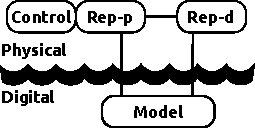
\includegraphics[width=300px]{mcrpd}}
	\caption{The MCRpd model of Ullmer \& Ishii for \acp{TUI}}
	\label{mcrpd}
\end{figure}

\acp{TUI} in general attempt to use the physical appearance of an object to communicate its virtual affordances \cite{Bellotti2002}. A user working with a \ac{GUI} only manipulates virtual objects, whereas \acp{TUI} allow the user to manipulate both physical and virtual objects, which coexist and share information with each other \cite{Shaer2004}. In a \ac{TUI}, the behaviour of a physical object is determined by the object's interactions with other physical and virtual objects - this is also the case in a smart environment.

Ullmer and Ishii \cite{Ullmer2000} extended the traditional \ac{MVC} model for \acp{TUI}, as shown in Figure \ref{mcrpd}. They distinguish between the physical and digital domains by placing the physical domain above the waterline, and the digital domain below the waterline. The model element is carried over from the \ac{MVC} model and represents the intangible digital information. The control element is also carried over from the \ac{MVC} model, while the view element is split into two subcomponents: 

\begin{itemize}
	\item Physical representations (Rep-p) -- represents the physically embodied elements of tangible interfaces
	\item Digital representations (Rep-d) -- represents the computationally mediated components of tangible interfaces without embodied form, for example video and audio, that can be observed in the physical world  
\end{itemize}

In a tangible interface, the physical representations (Rep-p) are computationally coupled to the underlying digital information (model), as well as perceptually coupled to the computationally mediated digital representations (Rep-d). The interaction model introduced in Section \ref{InteractionModel} was inspired by the \ac{MCRpd} model.

	
	
% \subsection{Foley's linguistic model}
% 
% 	Foley's model defines the following levels \cite{DeRuiter1988}:
% 	
% 	\begin{itemize}
% 		\item Conceptual level - definition of main concepts and the possible commands (equivalent to user model \cite{Buxton1983})
% 		\item Semantic level - defines the meaning of the commands
% 		\item Syntactic level - describes the form of the command and parameters (syntax)
% 		\item Lexical level - defines lowest input symbols and their structure
% 	\end{itemize}
% 	
% 	Buxton \cite{Buxton1983} extended Foley's model to include a pragmatic level that defines the issues of gesture type (e.g. pointing with a tablet versus a mouse), device location and spatial placement. While a keystroke will be defined at lexical level, the homing time and pointing time will be defined at pragmatic level. Buxton had the foresight to comment on the difficulty of multi-device environments where the different levels are managed by different entities. He noted that it has a strong effect on the semantics of the interactions that could be supported: If the computing environment is managed by one entity, the semantics and functional capabilities by another, and the user interface by yet another, there is an inherent danger that the decisions of the one will adversely affect the other. 
% 	
% 	Dix et al \cite{Dix2008} noted that Buxton's work emphasised the way in which the lexical level design of the physical interface can simplify syntax in interaction. These ideas have been extended by Ullmer et al \cite{Ullmer2005} into a \emph{digital syntax} that is embodied by the physical design, resulting in a grammar for mapping physical relationships into digital representations.
	
	% We build on the different interaction layers introduced here, that was later extended by Nielsen \cite{Nielsen1986} as described in Section \ref{nielsenVPM}, to categorise interaction events in Chapter \ref{EventModelling}.
	
\subsubsection{Arch/Slinky model}
	
	Bass et al \cite{Bass1992} contend that no single software architecture will satisfy all the design goals of an interactive system. With the Arch/Slinky model the buffering of a system from changes in technology was selected as the most important criterium. Here are some of the other design criteria they defined, which we consider to be especially important to ubiquitous computing systems:
	
	\begin{itemize}
		\item target system performance (e.g. size and speed)
		\item 	buffering from changes in application domain and hardware platform
		\item 	conceptual simplicity
		%\item 	complexity of specification
		\item 	target system extensibility
		\item 	compatibility with other systems
	\end{itemize}
	
	 They define an \emph{application} to be the total system that is developed for its end users, while the \emph{application domain} is the field of interest of, or reason for, the application. They also extended the definition of \ac{UIMS} to a  \ac{UIRS} - the runtime environment of an interactive application.
	
	The Arch model creates a bridge between the physical interaction device and the application domain. The following 5 components are defined:
	
	\begin{itemize}
		\item Interaction Toolkit Component - implements the physical interaction with the user (also called physical level)
		\item Presentation Component - provides a set of implementation-independent objects, e.g. a ``selector'' object can be implemented by both radio buttons or a drop-down menu in a GUI (also called lexical level)
		\item Dialogue Component - does task-level sequencing and maps between domain-specific and UI-specific formalisms (also called dialogue level)
		\item Domain Adaptor Component - triggers domain-initiated tasks, organises domain data, detects and reports semantic errors (also called functional core adapter)
		\item Domain-specific Component - controls, manipulates and retrieves domain data
	\end{itemize}

The separation of functionality into the different components was done to minimise the effects of changes in technology. The Slinky meta-model is a generalisation of the Arch model, providing a set of Arch models with different weights assigned to each component.

The difference between the Arch/Slinky model and our interaction model is that the  Arch/Slinky model relates a single physical interaction device with a software application, while our interaction model relates smart objects with one another through semantic connections.
% 
% \subsubsection{Nielsen's virtual protocol model}
% 
% \begin{table}
%     \myfloatalign
%   \begin{tabularx}{\textwidth}{Xll} 
% 	\toprule
%     \tableheadline{Level} & \tableheadline{Layer} & \tableheadline{Example} \\ 
%     \midrule
% 
% 	7 & Goal & Want to delete the last section of a document\\
% 	6 & Task & Delete the last six lines of the edited text\\
% 	5 & Semantic & Remove a line with a given line number\\
% 	4 & Syntax & DELETE 27 \\
% 	3 & Lexical & DELETE, DEL or other lexical token \\
% 	2 & Alphabetic & Letter ``D'' or other lexeme \\
% 	1 & Physical & User presses D-key on keyboard \\
% 	
%     \bottomrule
%   \end{tabularx}
%   \caption{Nielsen's virtual protocol model}
%   \label{VirtualProtocolModel}
% \end{table}
% 
% \label{nielsenVPM}
% Nielsen's virtual protocol model for human-computer interaction \cite{Nielsen1986} was inspired by the 7-layer OSI model for computer networks, as shown in Table \ref{VirtualProtocolModel}. The task layer deals with general computer-related concepts that are representations of the real world concepts from level 7, that may have to be realised by a sequence of operations from level 5. Level 5 handles the meaning of the interaction, where there are a finite number of concepts in the system and each have an exact definition. The lexical tokens on level 4 (``DELETE 27'') realises the semantic command ``remove a specific line''. Lexemes are information-carrying units that do not have any meaning by themselves. Screen layout could be considered a two-dimensional syntax that can also be defined in terms of lexical tokens. Direct manipulation \cite{Shneiderman1997} could be seen as using the syntax level to mirror the semantic level.
% 
% Nielsen compared his model to Foley's model and Buxton's extended version, as well as an earlier model by Moran called \ac{CLG} that consisted of six levels: task level, semantic level, syntactic level, interaction level and device level \cite{Nielsen1986}. He noticed that all models seem to agree on the visible (defining the form) part of the communication, as well as the invisible part (defining the meaning). Nielsen noted that Foley's model does not include the real-world concepts of his goal level, or the hardware-related detail of his physical level.
% 
% We build on the interaction layers of Nielsen to categorise interaction events in Chapter \ref{EventModelling}.







\subsubsection{The ASUR interaction model}
\label{theasurinteractionmodel}

\ac{ASUR} is a notation-based model to describe user-system interaction in mixed interactive systems \cite{Dubois2008} at design-time. It describes the physical and digital entities that make up a mixed system. \ac{ASUR} uses directed relationships to express physical and digital information flows, as well as the associations between components.

Both components and relationships may have characteristics. For components, this includes the location where the information is perceived (e.g. top of table) and action/sense required from the user (e.g. sight, touch or physical action). For relationships, characteristics include the dimensionality of the information (e.g. 2D or 3D) and the type of language used (e.g. text or graphics).

A sequence of such entities and their relationships in an interaction forms an \emph{interaction path}. The interaction exchange or action between elements in the path is conducted via one or more \emph{interaction channels} along which information or action is communicated. An interaction channel may be described in terms of its properties, either physical or digital depending on the channel, e.g. a digital channel may be described in terms of bandwidth, uptime and the nature of the connection. Adaptors are used transform information from the physical environment to the digital world and vice versa. An accelerometer for example may be modelled as a separate device, but if integrated into smart phones it can be abstracted away as part of an interaction path. 

Interaction carriers are mediating entities that are necessary for information communication. Passive carriers can carry and store part of the information communicated along an interaction path, e.g. a tangible object left in a particular position. Active carriers are transmitters of non-persistent information along the interaction path, e.g. a stylus used to transmit a precise position on a touch screen. Contextual entities are physical entities involved in an interaction (e.g. a table), and are also considered mediating entities.

The intended user model refers to what the user should know about the interaction in order to carry it out successfully. It may refer to one atomic interaction path (e.g. a channel, source and destination), or it may refer to more complex paths. 

An interaction group refers to a set of entities and channels that together have properties that are relevant to a particular design issue. Some of these groups will be applicable to any design, while others will depend on the task and context:

\begin{itemize}
\item Entities and channels may be \emph{grouped for feedback}, to identify an interaction flow that links the response of the system to the actions of the user.

\item User interface elements may be linked to application concepts in order to express a semantic association. The goal is to help the user to cognitively unify elements of the group (helping to establish the intended user model).

\item Sets of input (e.g. speech input for gesture input - ``put that there'') that must be combined to perform a certain task, may be grouped for multimodal interaction.

\item A grouping may be used to assert that a set of services must reside on the same machine or be distributed over multiple devices.

\item A grouping of paths may show information flows among or between multiple users.

\end{itemize}

An advantage of the \ac{ASUR} interaction model is that it combines both the physical and digital dimensions of user-system interaction. Later in Chapter \ref{SemanticConnectionsTheory} we will see how our interaction model also combines both these dimensions.

In this section we looked at how user interface software architectures can be used to model interactive systems. In the next section we look at how input devices can be modelled to describe the different interaction tasks that can be performed in a smart environment.

% Dubois and Gray \cite{Dubois2008} consider their interaction model similar to that of Coutrix et al \cite{Coutrix2006} (described in section \ref{mixedreality}), in the sense that both combine the physical and digital dimensions of the interaction. 
% 
% \subsubsection{The Mixed Reality interaction model}
% \label{mixedreality}
% 
% An interaction model aims at providing a framework for guiding designers to create interactive systems \cite{Coutrix2006}, characterised by their:
% 
% \begin{itemize}
% \item descriptive/classification power: describes existing interfaces and classifies them
% 
% \item generative power: helps designers create new designs
% 
% \item comparative power: helps to assess multiple design alternatives
% 
% \end{itemize}
% 
% Given that \emph{d} is a physical device that acquires or delivers information, and \emph{l} is an interaction language that defines a set of well-formed expressions that convey meaning, a modality \emph{m} is a pair \emph{(d,l)}. Modalities that define the link between digital and physical properties are known as \emph{linking modalities}, and modalities used by the user to interact with the mixed environment are known as \emph{interaction modalities}.
% 
% \begin{itemize}
% \item An input linking modality ($d_o^i, l_o^i$) is responsible for
% 
% \begin{enumerate}
% \item acquiring a subset of \emph{physical properties}, using a $d_o^i$ device (object input device)
% 
% \item interpreting these \emph{acquired physical data} in terms of \emph{digital properties}, using a language $l_o^i$ (object input language)
% 
% \end{enumerate}
% 
% \item An output linking modality is in charge of
% 
% \begin{enumerate}
% \item generating data based on the set of \emph{digital properties}, using a language $l_o^o$ (object output language),
% 
% \item translating these \emph{generated physical data} into perceivable \emph{physical properties} thanks to a device $d_o^o$ (object output device).
% 
% \end{enumerate}
% 
% \end{itemize}
% 
% An interaction language $l_i^i$ translates the digital properties of a mixed tool into elementary task to be performed (e.g. collect select puzzle piece). Using the linking modalities, different modalities may be generated to describe the mixed tool.

	
\section{Modelling input devices} 
\label{interactionTasks}

\subsection{Foley's taxonomy and its extensions}
	
	Foley \cite{Foley1984} describes a taxonomy of input devices that are structured according the graphic subtasks they can perform: position, orientation, select, path, quantify and text entry. He defined these subtasks as six \acp{BIT}. A \ac{BIT} is the smallest unit of information entered by a user that is meaningful in the context of the application. He noted that there are far too many interaction techniques to give an exhaustive list, and that it is impossible to to anticipate which new techniques may be created. In Table \ref{InteractionTasks} we map them to possible logical and physical interaction devices. The six types of logical devices were also defined by Foley in \cite{Foley1996}.
	
	
	\begin{table}
	    \myfloatalign
	  \begin{tabularx}{\textwidth}{Xll} 
		\toprule
	    \tableheadline{Interaction Task} & \tableheadline{Logical Device} & \tableheadline{Physical Device} \\ 
	    \toprule

		Position & Locator & Tablet \\
		\cline{1-2}

		\multirow{2}{*}{Select} & Choice & Touch Panel\\
		 						& Pick & Trackball/Mouse\\
		\cline{1-2}						
		Path & Stroke & Joystick \\
		\midrule
		Quantify & Valuator & Dials\\
		\midrule
		Text entry & String & Keyboard  \\
		\midrule
		Orient & & \\

	    \bottomrule
	  \end{tabularx}
	  \caption{Interaction tasks mapped to logical and physical interaction devices}
	\label{InteractionTasks}
\end{table}
	

	
	Some characteristics of the physical interaction devices are not shown in the table.  The positioning of tablets and touch panels are \emph{absolute}, while that of trackballs, joysticks and mice are \emph{relative}. A touch panel is considered \textit{direct}, as the user directly points at the screen, while a tablet is \textit{indirect}. Joysticks, tablets and mice are \emph{continuous}, while a keyboard is \emph{discrete}. Dials can either be \emph{bounded} or \emph{unbounded}.
	
	The \emph{positioning} interaction task involves specifying an (x,y) or (x,y,z) position. Characteristics of this task include different coordinate systems, resolution and spatial feedback. The \emph{select} interaction task involves choosing an element from a choice set, while the \emph{text} interaction task entails entering character strings to which the system does not assign specific meaning. The \emph{quantify} interaction task involves specifying a numeric value between some minimum and maximum value. The \emph{path} interaction task consists of specifying a number of positions over a specific time or distance interval. The \emph{orient} interaction task is also called \emph{rotate}, but is not often used \cite{DeRuiter1988}.
	
	Card et al \cite{Card1991} argued that the Foley taxonomy has not tried to define a notion of completeness, and is thus not generic enough. They pointed out that single devices appear many times in the levels of the tree, which makes it difficult to understand the similarities among devices. MacKinlay, Card and Robertson \cite{MacKinlay1990} extended Buxton's work to propose additional physical properties that underly most devices. They follow mappings from the raw physical transducers of an input device into the semantics of the application.
	
	Dix et al \cite{Dix2008} noted that Card et al's analysis is not only relevant to GUIs, as they used a running example of a radio with knobs and dials. Their work not only abstracts devices into classes, but also takes into account that rotating a dial is different from moving a slider, i.e. the physical nature of the interaction is also important.
	
	 Ballagas et al \cite{Ballagas2006} surveyed interaction techniques that use mobile phones as input devices to ubiquitous computing environments, and used Foley's six interaction tasks as a framework for their analysis. In their work on iStuff \cite{Ballagas2003} they state that the set of interactions tasks are only sufficient for describing graphical user interfaces, not physical user interfaces, or user interfaces in general. The same paper notes that Buxton's taxonomy, and the extension by MacKinlay, Card and Robertson, is too narrow for ubiquitous computing environments, as it does not classify devices with different modalities and only describes input devices. They extended the taxonomy further to describe attributes like direction and modality. The direction attribute is used to indicate whether a device provides input, output or both. The modality attribute describes different visual, auditory haptic and manual modalities for input and output. Additional attributes they identified include directionality/scope (where a device is targeted to one, many, or all the users in a room) and mount time (the effort necessary to use an interaction device).

Based on the work of Foley, Card and others in this section, we defined a concept called the \emph{interaction primitive}, described in more detail in Section \ref{sectionSemanticInteractionOntology} and \ref{InteractionPrimitives}. Interaction primitives can be used as a way to describe the user interaction capabilities of smart objects in ubiquitous computing environments.
	
% \subsection{Another approach to task modelling: ANSI/CEA-1028}
% \label{cea2018}
% 
% 	A task model is often defined as a description of an interactive task to be performed by the user of an application through the application's user interface. Individual elements in a task model represent specific actions that the user may undertake. Information on subtask ordering as well as conditions on task execution is also included in the model~\cite{Limbourg2004}. In traditional user interface design, task models are used only at design time and then discarded \cite{Rich2009}. A task-based user interface uses a task model at runtime to guide the user.
% 
% 	A task is commonly defined as an activity performed to reach a certain goal. A goal of a task is considered to be a specific state that is reached after the successful execution of a task. Tasks vary widely in their time extent. Some occur over minutes or hours (like listening to a song or watching a TV show), while others are effectively instantaneous, like switching on the TV.
% 
% 	ANSI/CEA-1028 \cite{Rich2009} uses a single uniform task representation, compared to other representations where high-level tasks (goals) are separated from low-level tasks (actions). It does so at all levels of abstraction, providing more flexibility when adjusting the level of granularity. %We consider this a worthwhile option to explore as this allows for the simplification of the model.
% 
% 	In \cite{VanWelie1998} it is suggested that task models should be based on an ontology that describes the relevant concepts and the relationships between them, independently of any used graphical representations. This also allows for different visualisations of the same task model. Task decomposition is the most common ingredient of task models. This creates a task tree or hierarchy that can easily be modelled by an ontology. The most important purpose of a task is that it changes something, otherwise it has no reason for existing.
% 
% \marginpar{Van Welie et al \cite{VanWelie1998} state that task models should be able to represent the psychological, social, environmental and situational aspects of agents and their tasks. This is why we consider runtime task models a good fit for the \ac{BDI} model used for constructing intelligent agents.}
% 	

While we these techniques are well suited to modelling input devices, we still need a way to describe the semantics of interaction feedback and the different types of interactions that can occur. That is the focus of the next section on semantic models.	

\section{Semantic models}
\label{SemanticModels}
\subsection{The Frogger framework}
\label{interactionFrogger}
The Frogger framework, as was introduced by Wensveen \cite{Wensveen2005}, describes user interaction in terms of the information a user perceives (like feedback and feedforward), and the nature of this information. It distinguishes between inherent, augmented and functional information. These types of information can serve as couplings between user actions and the systems' functions in time, location, direction, modality, dynamics and expression. Although the framework was designed to describe the interaction with electronic devices and their interfaces, many of the concepts in the framework are applicable to interactions with systems of devices as well.

When a user performs an action and the device responds with information that is directly related to the function of that product (lighting switching on when a light switch is operated), we speak of \emph{functional feedback}. When a device has more than one functionality, functional feedback should be viewed with respect to the users' intentions and goals when performing the action. If there is no direct link between a user's action and the direct function of the product, or when there is a delay, \emph{augmented feedback} (also known as indicators \cite{Thimbleby2007}) can be considered to confirm a user's action. This feedback is usually presented in the form of lights, sounds or labels. \emph{Inherent feedback} is directly coupled (inherently) to the action itself, like the feeling of displacement, or the sound of a button that is pressed.

While feedback is information that occurs after or during the interaction, feedforward is the information provided to the user before any action has taken place. \emph{Inherent feedforward} communicates what kind of action is possible, and how one is able to carry out this action. Inherent feedforward is the same as the concept of affordances\marginpar{Affordances were discussed in Section \ref{Affordances}. }, revealing the action possibilities of the product or its controls \cite{Wensveen2005}. When an additional source of information communicates what kind of action is possible it is considered \emph{augmented feedforward}.  
\emph{Functional feedforward} communicates the more general purpose of a product. %This type of information often relies on association, metaphors and the sign function of products, which are described by theories such as product semantics \cite{Krippendorff2006}. Good practice in creating inherent feedforward is making the functional parts of a product visible, informing users about the functionality of the product \cite{Norman1998}.	

%\footnote{Affordance is a term coined by Gibson in 1979 and introduced to the design community by Norman \cite{Norman1998}. It is the property of an object that appeals to our sensory-motor skills, like a door handle ``affords'' to be grabbed and a chair ``affords'' to be sat on.}

The concepts described in the Frogger framework are used to implement feedback and feedforward in the work described in this thesis, specifically in Section \ref{section:feedbackAndFeedforward} and Section \ref{feedbackforward}. 
	
\subsection{Models of intentionality}
\label{intentionalSpectrum}
	
	At the semantic level, we are interested in the meaning of the action. A gesture may mean nothing, until it encounters for instance a light switch \cite{Bongers2007}. In traditional software applications, a user is expected to have a clear intention of what he/she wants to achieve, with purposeful and direct actions. In ubiquitous computing scenarios, the interactions are less explicit. Input can be implicit, sensor-based and ``calm'', and output is ambient and non-intrusive. With \emph{incidental interactions} \cite{Dix2004}, a user performs an action for some purpose (say opening a door to enter a room), the system senses this and incidentally uses it for some purpose of which the user is unaware (e.g. adjust the room temperature), affecting the user's future interaction with the system.
	
\begin{figure}
	\centering
	\centerline{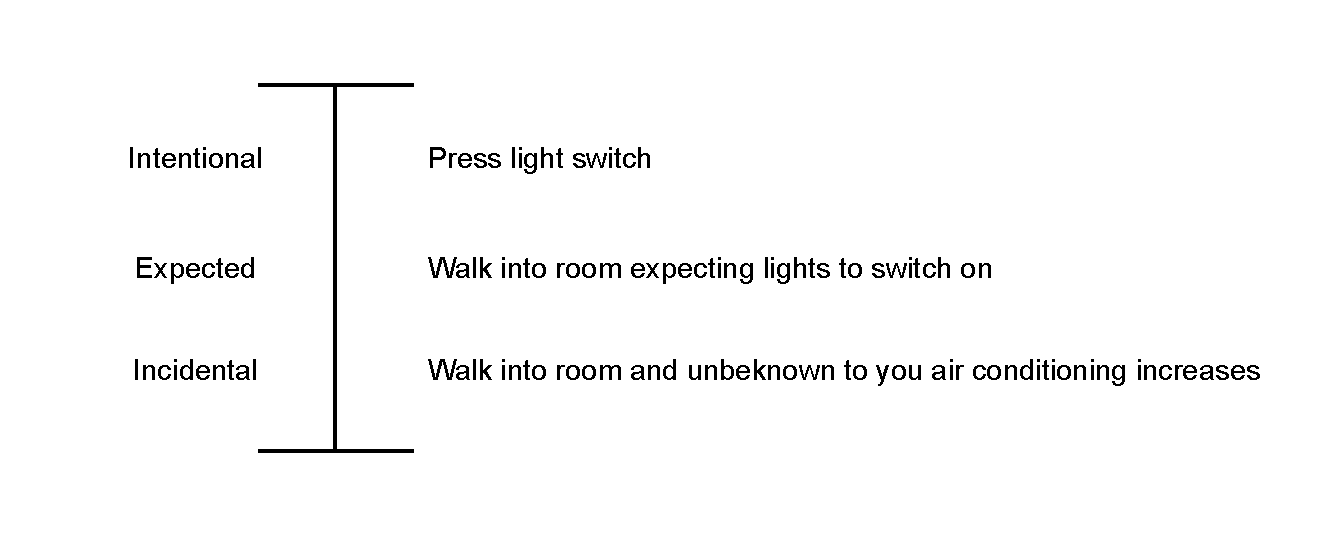
\includegraphics[width=300px]{continuum}}
	\caption{The continuum of intentionality}
	\label{continuum}
\end{figure}	

	The \emph{continuum of intentionality} in Figure \ref{continuum} has normal, intentional interactions at the one end of the spectrum (e.g. pressing a light switch), expected interactions in the middle (e.g. walking into a room expecting the lights to go on), and incidental interactions at the other end. As users become more aware of the interactions happening around them, they move through the continuum toward more purposeful interaction. For example, with \emph{comprehension} an incidental interaction (lights turning on when you enter the car) turns into an expected interaction. With \emph{co-option}, an expected interaction turns into an intended interaction (e.g. deliberately opening and closing the car door to turn on the light).

	Incidental interactions do not fit existing interaction models based on the conventional intentional cycle, like Norman's Action Cycle Diagram \cite{Norman1998}. The purpose of the user's activity is distinct to the intended outcomes of the system. Feedback may be unobtrusive (and not noticed), or delayed (like the temperature slowly changing). There are two tasks that are occurring: The user's purposeful activity, and the task that the incidental interaction is attempting to support/achieve.

We try to improve this comprehension by actively involving users in configuring the relationships between the smart objects in their environment. Bellotti et al. \cite{Bellotti2002} posed five questions to the designers of ubiquitous computing technologies:

\begin{itemize}
	\item Address: How do I address one (or more) of many possible devices?
	\item Attention: How do I know the system is ready and attending to my actions?
	\item Action: How do I effect a meaningful action, control its extent and possibly specify a target or targets for my action?
	\item Alignment: How do I know the system is doing, or has done, the right thing?
	\item Accident: How do I avoid mistakes?
\end{itemize}

When users are able to explore and manipulate the relationships between the smart objects, it becomes easier for them to begin to comprehend how things work, or can potentially work together. They can project their experiences with a part of a smart environment to see what may potentially work for other parts of the environment as well. 
By allowing users to configure their smart environment themselves, they are in control of deciding how the environment responds to their actions. By making use of the feedback mechanisms introduced in Section \ref{interactionFrogger} we can indicate that the system is ready and attending to a user's actions. These mechanisms can also be used to make the action possibilities of the system more visible and help the user avoid mistakes.

%end TiiS

\section{Outlook}

As Nielsen \cite{Nielsen1986} noted, the purpose of a model is to improve the usability of software. He noted that some people will consider a model a useful abstraction, while others will prefer other models, similar to how everybody has their own favourite programming language.

We build further on many of the concepts and proposals reviewed in this chapter. In particular, we focus on configuring the connections between the devices in Chapters \ref{DesignIteration1} to \ref{DesignIteration3} and Chapter \ref{SemanticConnectionsTheory}, while serendipitous interoperability and sharing information between devices form the cornerstones of Chapter \ref{DeviceCapabilityModelling} and Chapter \ref{EventModelling}. 



\cleardoublepage
\ctparttext{You can put some informational part preamble text here. 
Illo principalmente su nos. Non message \emph{occidental} angloromanic
da. Debitas effortio simplificate sia se, auxiliar summarios da que,
se avantiate publicationes via. Pan in terra summarios, capital
interlingua se que. Al via multo esser specimen, campo responder que
da. Le usate medical addresses pro, europa origine sanctificate nos se.}
\part{Design iterations and constructing a theory}
\chapter{Design iteration I}
\label{DesignIteration1}

\begin{flushright}{\slshape    
I think the only way forward is going from applying algorithms to\\
individual transactions, to first placing information in \\
context --- pixels to pictures --- and only applying algorithms \\
after one sees how the transaction relates to the other data.\\
It's the only way that I can see that it's going to close this\\
 sense-making gap.} \\ \medskip
    --- Jeff Jonas \cite{AlexWoodie}
\end{flushright}


\marginpar{Parts of this chapter appear in \cite{Niezen2010} and \cite{VanderVlist2010}.}

An iterative development process was followed for the work described in this thesis. In the following chapters three iterations, each consisting of a requirements and planning phase, analysis and design phase, implementation phase and evaluation phase, is described in more detail. Iterative processes are essential to modern-day software and hardware development methodologies, exemplified by the various agile development frameworks \cite{Larman2003}.

\section{Requirements}

The goal of the first design iteration was to see if using a tangible interface to establish connections between devices is a viable alternative to the usual \ac{GUI}-based solutions. Additionally, different approaches to modelling user interaction, device capabilities and connections were explored.

Scenarios are commonly used in software engineering and interaction design to help discover and analyse requirements. The following scenario was presented at the start of the project to guide the design process:

\emph{Mark is a 12-year-old boy and he is at home receiving his friend Dries from school. Dries arrives with a portable music player loaded with his favourite songs. He wants to play some recent collections for Mark. Mark's home is equipped with a sophisticated surround sound system, and they have recently installed an ambient lighting system that is connected to the sound system and renders the mood of the music by dynamic colour lighting in the room. They decide to use both to enjoy the music. Dries starts streaming his music to the environment.}

\emph{An object (or several objects) shows possible input and output ports for streaming music in the environment. By interaction with the object/objects, Mark connects the output from Dries' music stream to the input of the sound system. Now the room is full with Dries' music and the colourful lighting effects. Mark's mom, Sofia, now comes back from work. She starts preparing dinner for the family. Mark and Dries don't want to bother her with their loud music. They again use the object(s) to re-arrange the music stream. Now the music is streamed to Mark's portable music player while playing back at Dries'. It is also connected to the ambient lighting system directly, bypassing the sound system. They both are enjoying the same music using their own favourite earphones, and the colourful lighting effects, but without loud music in the environment.}

\emph{The object(s) shows the connection possibilities with a high level of semantic abstraction, hiding the complexity of wired or wireless networks. By interacting with the object(s), semantic connections can be built, redirected, cut or bypassed.}

The first takeaway from this scenario is that the focus is on the connections between the devices, instead of on the devices themselves. This brings us to the first design decision: \emph{Semantic connections} are introduced as a means to indicate users' intentions concerning the information exchange between smart objects in a smart environment. 


\begin{description}
	\item [Semantic Connection] A semantic connection is a relationship between two entities in a smart environment for which we focus on the semantics---or meaning---of the connections between these entities. 
\end{description}

The term semantic connections is used to refer to meaningful connections and relationships between entities in a smart environment. These connections are both real ``physical'' connections (e.g. wired or wireless connections that exist in the real world) and ``mental'' conceptual connections that seem to be there from the user's perspective. The context of the connections, for example the objects that they connect, provide meaning to the connections. The term ``semantics'' refers to the meaningfulness of the connections. The type of connection, which often has the emphasis now (e.g. WiFi, Bluetooth or USB) is not considered to be the most relevant, but what the connection can do for someone --- its functionality --- even more.

%end S3E
The following requirements were defined during this phase:

\begin{itemize}
	\item Semantic connections exist in both the physical and the digital world. We need ways to visualise these invisible connections and to control them. 
	\item Devices need to be able to share their capabilities and content with the other devices in their environment.
\end{itemize}

A number of different approaches to visualising and controlling semantic connections were explored in the first iteration, and these are described in Section \ref{DeviceDesign1}. We also need a way to model the devices, their capabilities and the connections themselves. This is the subject of the next section.



% ``Mark is relaxing at home when his friend Dries arrives. Dries comes with a portable music player loaded with his favourite songs. He wants to play some of his recent collections for Mark. Mark's home is equipped with a sophisticated surround sound system. They decide to enjoy the music from the music player on the sound system. Mark uses his Interaction Tile to see if he can connect Dries's music player to the sound system, which is connected to the home network. The interaction tile indicates that a connection is possible and Mark picks up the tile and shakes it to make the connection.
%  
% All the smart devices in the home have a cube-like representation that can be used with the interaction tile. The interaction tile shows the connection possibilities with a high level of semantic abstraction, hiding the complexity of the wired or wireless networks. By interacting with the objects, semantic connections can be built, redirected, cut or bypassed.
% 
% Dries starts streaming his music to the environment. Now the room is full with Dries's music and they both enjoy listening to it. Recently Mark has installed an ambient lighting system that can be connected to the sound system and renders the mood of the music by dynamic colour lighting in the room. Mark uses the objects again to create another connection and now the room is filled with Dries's music and colourful lighting effects.
% 
% Mark's roommate Sofia comes back from work and decides she wants to watch a movie on the TV. She seems somewhat annoyed by the loud music. Mark and Dries do not want to bother her and they again use the objects to re-arrange the music stream. Now the music is streamed to Mark's portable music player while also playing back at Dries's. It is also connected to the ambient lighting system directly, bypassing the sound system. They both are enjoying the same music using their own favourite earphones (and the colourful lighting effects), but without loud music in the environment. Now Sofia can enjoy her movie without any disturbing music.''

%From this scenario one can see that there are multiple ways and different levels of interacting with the devices in the environment. There are high-level semantic interactions with the interaction tile (explore/make/break connections) and also lower-level interactions with the music player (play/pause/stop music).




\section{Ontology Design}
\label{OntologyDesign1}

\ac{OWL} 2, the ontology language used to build ontologies for the Semantic Web, was used to create the ontologies in this thesis. \ac{OWL} 2 has been a W3C Recommendation since October 2009, and adds new capabilities like property chains to the original \ac{OWL} standard. % Possible TODO find more on why OWL 2
\marginpar{Ontologies and ontology engineering are described in more detail in Section \ref{OntologyEngineering}. }

\begin{figure}[bth]
	\digraph[scale=0.45]{ontology1}{
	rankdir=RL;
		Thing [label="owl:Thing"];
		SmartObject -> Thing;
		Event -> Thing;
		NFCEvent -> Event;
		NFCEnterEvent -> NFCEvent;
		NFCExitEvent -> NFCEvent;
		NetworkEvent -> Event;
		ConnectEvent -> NetworkEvent;
		DisconnectEvent -> NetworkEvent;
		MediaPlayerEvent -> Event;
		PlayEvent -> MediaPlayerEvent;
		CueEvent -> MediaPlayerEvent;
		StopEvent -> MediaPlayerEvent;
	}
	\caption{Ontology indicating subclass relationships}
	\label{ontology1}
\end{figure}

% \begin{figure}[!t]
% \centering
% 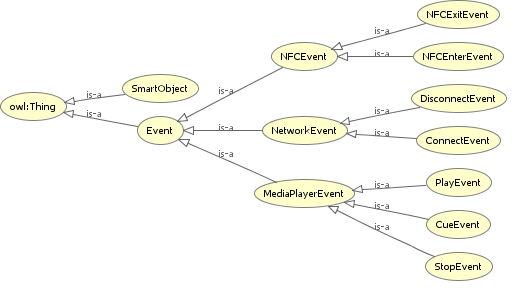
\includegraphics[width=200pt]{Ontology}
% \caption{Ontology indicating subclass relationships}
% \label{ontology1}
% \end{figure}

A first attempt at modelling the various entities in an ontology is shown in Figure \ref{ontology1}. A bottom-up approach to modelling was used, where we attempted to model each entity using the least number of statements. These entities were later aligned with foundational ontologies -- the approach that was followed is discussed further in Chapter \ref{OntologyEngineering}. Each entity is modelled as an \texttt{owl:Class}, where all classes are subclassed from the root class, \texttt{owl:Thing}\footnote{The \texttt{owl:} prefix is used to denote the \ac{OWL} 2 Namespace Document located at \texttt{http://www.w3.org/2002/07/owl}.}. Each edge in the graph above is an \texttt{rdf:type} relationship, and the direction of the arrow indicates the direction of the subclass relationship.

During the initial development stages, we realised that the most promising way of describing low-level interactions seemed to be to describe them in terms of \emph{interaction events}, that are defined as follows:\marginpar{Interaction events are discussed in more detail in Chapter \ref{EventModelling}.}

\begin{description}
	\item [Interaction event] An interaction event is defined as an event that occurs at a certain time instant and was generated by a specific smart object. It reports either the intent of a user's action directly, or a perceivable change in a smart object's state.
\end{description}

An interaction event in the smart space consists of an event ID, timestamp and other related information, like the smart object that generated that event. For the scenario, three types of interaction events were defined:

\begin{itemize}
	\item Network events: A \texttt{ConnectEvent} indicates that a device is entering the smart space, while a \texttt{DisconnectEvent} means that the device is exiting the smart space. 
	\item \ac{NFC} events: An \texttt{NFCEnterEvent} signifies that an \ac{NFC} tag has entered the \texttt{RFID} field, and a \texttt{NFCExitEvent} is generated when it leaves the field.
	\item Media player events: When the user presses the Play button on the media player, a \texttt{PlayEvent} is generated. When the music is stopped, or at the end of the song, a \texttt{StopEvent} is generated. Pressing the Forward button forwards the song by 5 seconds. This time period is attached to a \texttt{CueEvent} using an \texttt{atTime} relationship.
\end{itemize}

The following properties were defined:\marginpar{All \ac{OWL} code listings in this thesis are written using Turtle\footnote{http://www.w3.org/TeamSubmission/turtle/} syntax. Turtle is a human-friendly alternative to \ac{XML} based syntaxes.}

\begin{minted}{turtle}
	:connectedTo
	    a owl:ObjectProperty;
	    a owl:IrreflexiveProperty;
	    a owl:SymmetricProperty ;
	    rdfs:domain :SmartObject ;
	    rdfs:range :SmartObject .

	:atTime
	    a owl:DatatypeProperty ;
	    rdfs:comment "At a specific time (in milliseconds)";
	    rdfs:range xsd:integer .

	:generatedBy
	    a owl:ObjectProperty ;
	    rdfs:domain :Event ;
	    rdfs:range :SmartObject .

	:hasPosition
	    a owl:DatatypeProperty ;
	    rdfs:range xsd:integer .

	:hasRFIDTag
	    a owl:DatatypeProperty ;
	    rdfs:range xsd:string .

	:inXSDDateTime
	    a owl:DatatypeProperty ;
	    rdfs:range xsd:dateTime .
\end{minted}


The \texttt{connectedTo} object property is both \emph{symmetric} and \emph{irreflexive}. Irreflexive properties are a new feature in \ac{OWL} 2. A symmetric property is its own inverse, which means that if we indicate a \texttt{connectedTo} relationship from device A to device B, device B will also have a \texttt{connectedTo} relationship to device A. Another way to think of symmetric properties is that they are bidirectional relationships. 

An irreflexive property is a property that never relates an individual to itself \cite{Hebeler2009}. This allows us to restrict our model by not allowing a \texttt{connectedTo} relationship from a device to itself.


An example with individuals, also called instances, that make use of the ontology is shown in Figure \ref{ontologyInstance}. In the figure, classes are denoted with ellipses, individuals with boxes and datatypes as plain text. Class membership is denoted with dotted lines and relationships are denoted with solid lines. It shows a Nokia N900 and N95 smartphone instantiated as \texttt{SmartObjects} with their associated \ac{RFID} tags.\marginpar{Why an \ac{RFID} tag? in Section \ref{Identification} we argue that that each smart object must be uniquely identifiable in the physical world by digital devices.}

An instantiated \texttt{NFCExitEvent}, called \texttt{event-1cecdba5}, is also shown. When an event is generated a \ac{UUID} is assigned to it, to enable the event to be uniquely identified in the smart space. It is also associated with a smart object using the \texttt{generatedBy} property. The \texttt{hasPosition} relationship provides additional metadata required by the interaction tile, which is described in the next section.  

\begin{figure}[bth]
	\centerline{
	\digraph[scale=0.45]{ontologyInstance}{
		rankdir=LR;
		node[shape="box"];
		event1 [label="event-1cecdba5"];
		date [label="2009-12-17T13:15:16^xsd:dateTime", shape="plaintext"];
		position [label="2^xsd:integer", shape="plaintext"];
		SO [label="SmartObject", shape="ellipse"];
		Event [label="NFCExitEvent", shape="ellipse"];
		rfid1 [label="04A332D9A12580"];
		rfid2 [label="0401C4D9A12581"];
		event1 -> Event [style="dotted"];
		event1 -> date [label="inXSDDateTime"];
		event1 ->  position [label="hasPosition"];
		event1 -> NokiaN900 [label="generatedBy"];
		NokiaN900 -> AmbientLighting [label="connectedTo"];
		NokiaN900 -> rfid1 [label="hasRFIDTag"];
		NokiaN900 -> SO [style="dotted"]; 
		AmbientLighting -> NokiaN900 [label="connectedTo"];
		AmbientLighting -> rfid2 [label="hasRFIDTag"];
		AmbientLighting -> SO [style="dotted"];
	}}
	\caption{Individuals that were instantiated based on the ontology}
	\label{ontologyInstance}
\end{figure}


\ac{SPARQL}\footnote{http://www.w3.org/TR/rdf-sparql-query/} form the query language for the Semantic Web. Along with \ac{OWL}, it is one of the core technologies of the Semantic Web, having been a W3C Recommendation since January 2008. \ac{SPARQL} queries are based on the idea of graph pattern matching \cite{Sequeda2012}, where data that is returned from the query is set to match the pattern.\marginpar{We also make use of \ac{SPARQL} to define rules, which is described in Section \ref{SPIN}.}

To determine which other smart objects a specific device, for example a mobile phone, is connected to, a simple \ac{SPARQL} query suffices:

\begin{minted}{sparql}
SELECT DISTINCT ?object WHERE {
:phone1 :connectedTo ?object .
}
\end{minted}

\label{Jena}
A \emph{triple store} is used to store both the instances and the ontology. A triple store is a purpose-built database for storing and retrieving triples, in the format subject-predicate-object. In the above example \emph{phone1} would be the subject, \emph{connectedTo} the predicate and \emph{?object} the object. There are a number of commercial and open-source triple store implementations. The Jena\footnote{http://jena.apache.org/} framework is a Java \ac{API} that enables access to many triple store implementations, supports \ac{SPARQL} and also has its own persistent triple store. It was used in this first implementation and was also later adopted by the \ac{SOFIA} project.

An advantage of using \ac{SPARQL} and a triple store is that it is easy to add additional constraints and/or specifics to the query, compared to a traditional \ac{SQL} database, where unions between columns and tables can get quite complicated very quickly.

To get the last event that was generated by a specific device, the \ac{SPARQL} query is a little bit more complex, but still surprisingly manageable:

\begin{minted}{sparql}
SELECT ?event ?eventType WHERE { 
:deviceID :hasRFIDTag ?tag . 
?event :hasRFIDTag ?tag .
?event a ?eventType . 
?event :inXSDDateTime ?time . 
FILTER (?eventType = :NFCEnterEvent  || ?eventType = :NFCExitEvent) 
} 
ORDER BY DESC(?time) 
\end{minted}

%Instances in the triple store could be considered to form part of the \ac{BDI} beliefs of an agent, from the \texttt{connectedTo} relationships between the smart objects, to interaction events that occurred in the past. If we describe a sequence of actions (plan) in the ontology to achieve a certain intention, we may then use the interaction events to trigger the plan, update beliefs or modify goals. Goals may be defined in the ontology as desires, where we can add the necessary property restrictions to ensure that active desires are consistent. If sequences of actions are sufficiently defined in the ontology, we may even be able to use a reasoner to infer subsumption hierarchies of plans based on the user's current actions, which in turn would allow us to determine the user's intentions.

\marginpar{Semantic data focuses on the relationships between entities, making semantic models property-oriented. Entities are members of a class based on their properties/predicates.}
How do we model the semantic connections between devices? Since semantic modelling is property-oriented instead of object-oriented\cite{Segaran2009a}, we started by focusing on the possible predicates that can be used to describe connections. We need a way to model whether a connection is possible --- this can be done with a \texttt{canConnectTo} property. We also need to know if a device is currently connected to another device --- \texttt{connectedTo}. Then we need a way to model the capabilities that each device provides. In this first iteration, we defined two properties called \texttt{consumes} and \texttt{provides}. They are used as follows:

\begin{minted}{turtle}
	NokiaN900 provides AudioCapability .
	NokiaN95 consumes AudioCapability .
\end{minted}

During the later design iterations we decided to model capabilities as functionalities of a device instead, and make the name of the property clearer to indicate whether it is a functionality of a source or a sink. The property \texttt{provides} was changed to \texttt{functionalitySource}, and \texttt{consumes} was changed to \texttt{functionalitySink}. These early properties are mentioned here for the sake of completeness, and to show how aspects of the ontology have changed between iterations.

% \begin{tabular}{cc}
% 	Iteration 1 (08/09) & Final iteration \\
% 	canConnect & canConnectTo \\
% 	isConnected & connectedTo \\
% 	provides & functionalitySource \\
% 	consumes & functionalitySink \\
% \end{tabular}


\section{Device design}
\label{DeviceDesign1}

Based on the scenario, a number of smart objects had to be constructed or repurposed, and the necessary software had to be developed.

To explore the different possibilities of visualising and manipulating connections between devices, a number of different prototypes were constructed. The first of these is called the \emph{interaction tile}. 

%- Components used: Interaction Tile, Lamp
%- 5800 (\euro 265) as cheap phone with WiFi


\subsection{Interaction Tile}
\label{InteractionTile}

\begin{figure}[bth]
\centering
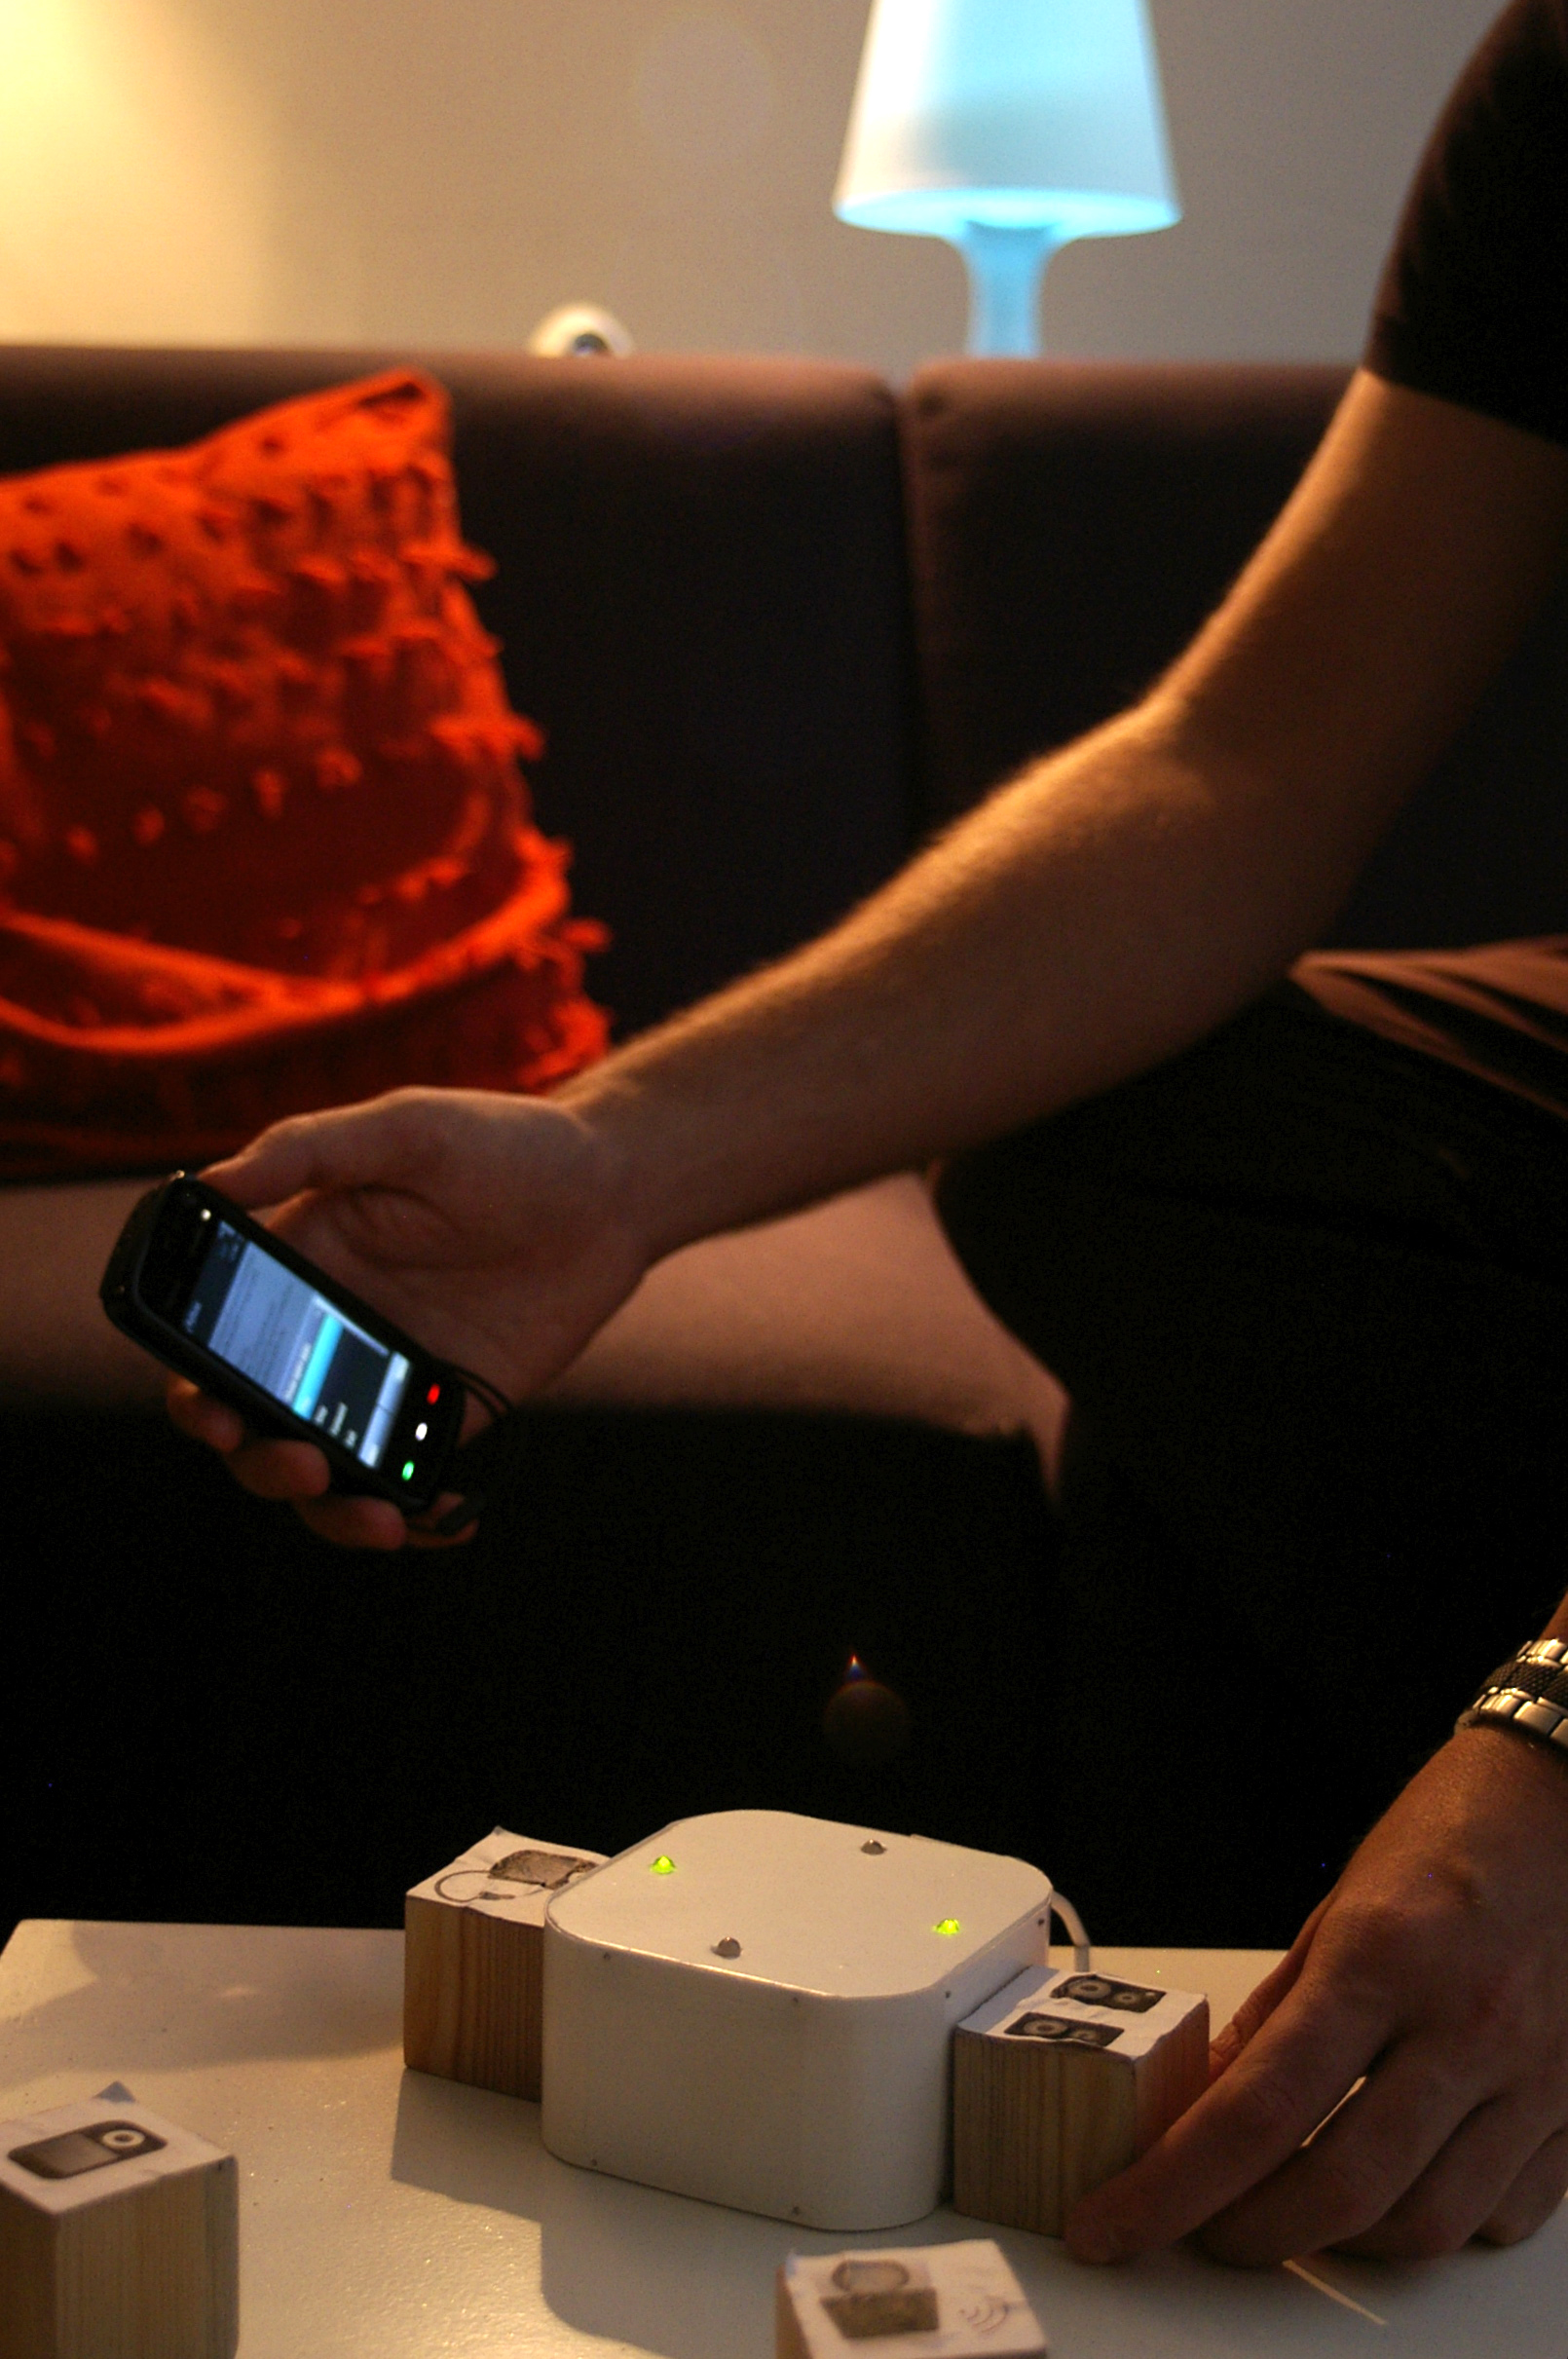
\includegraphics[width=260pt]{tile1}
\caption{The interaction tile and mobile phone}
\label{tile1}
\end{figure}

The interaction tile, shown in Figure \ref{tile1}, was inspired by Kala\-nithi and Merrill's ``Siftables'' cubes \cite{Merrill2007}. It was designed to explore and manipulate connections through direct manipulation -- by making simple spatial arrangements. Each device in the smart environment is represented by a cube containing an \ac{RFID} tag and a small magnet, with an icon on the top of the cube to signify the device being represented. When a cube is placed next to one of the four sides of the tile, an LED on the tile lights up to indicate that it has been recognised. When a second cube is placed next to the tile, the following LED visualisations are used:

\begin{itemize}
	\item Pulsating green light - a connection is possible
	\item Constant green light - a connection exists
	\item Red light - no connection is possible
\end{itemize}  

The interaction tile visualises the various connections by allowing a user to explore which objects are currently connected, and what connections are possible. By means of putting a cube representing a device close to one of the four sides of the tile, a user can check if there is a connection, and if not, whether a connection is possible. By shaking the tile it is possible to create a connection between two devices, or where there is an existing connection, to break the connection. The interaction tile consists of the following components:

\begin{itemize}
	\item Arduino Duemilanove with Atmel ATMega328 microcontroller
	\item ACR122/Touchatag 13.56MHz \ac{RFID} reader
	\item RF Solutions ANT-1356M 13.56MHz \ac{RFID} Antenna Coil
	\item Multi-colour LEDs
	\item Accelerometer 
	\item Vibration motor
	\item Piezoelectric speaker
	\item Magnetic switches
\end{itemize}

The Arduino communicates with a PC via a serial interface over USB, while the \ac{RFID} reader uses \ac{PC/SC} drivers over USB.\marginpar{The \ac{RFID} reader component has been tested under Windows, Linux and Mac OS X.} The accelerometer is used to measure when the user is shaking the tile, while the vibration motor and speaker provide haptic and auditory feedback. The magnetic switches are used to determine which side of the tile a cube has been placed. The final laser-cut version of the interaction tile prototype is shown in \mbox{Figure \ref{tile2}}.

\begin{figure}[bth]
\centering
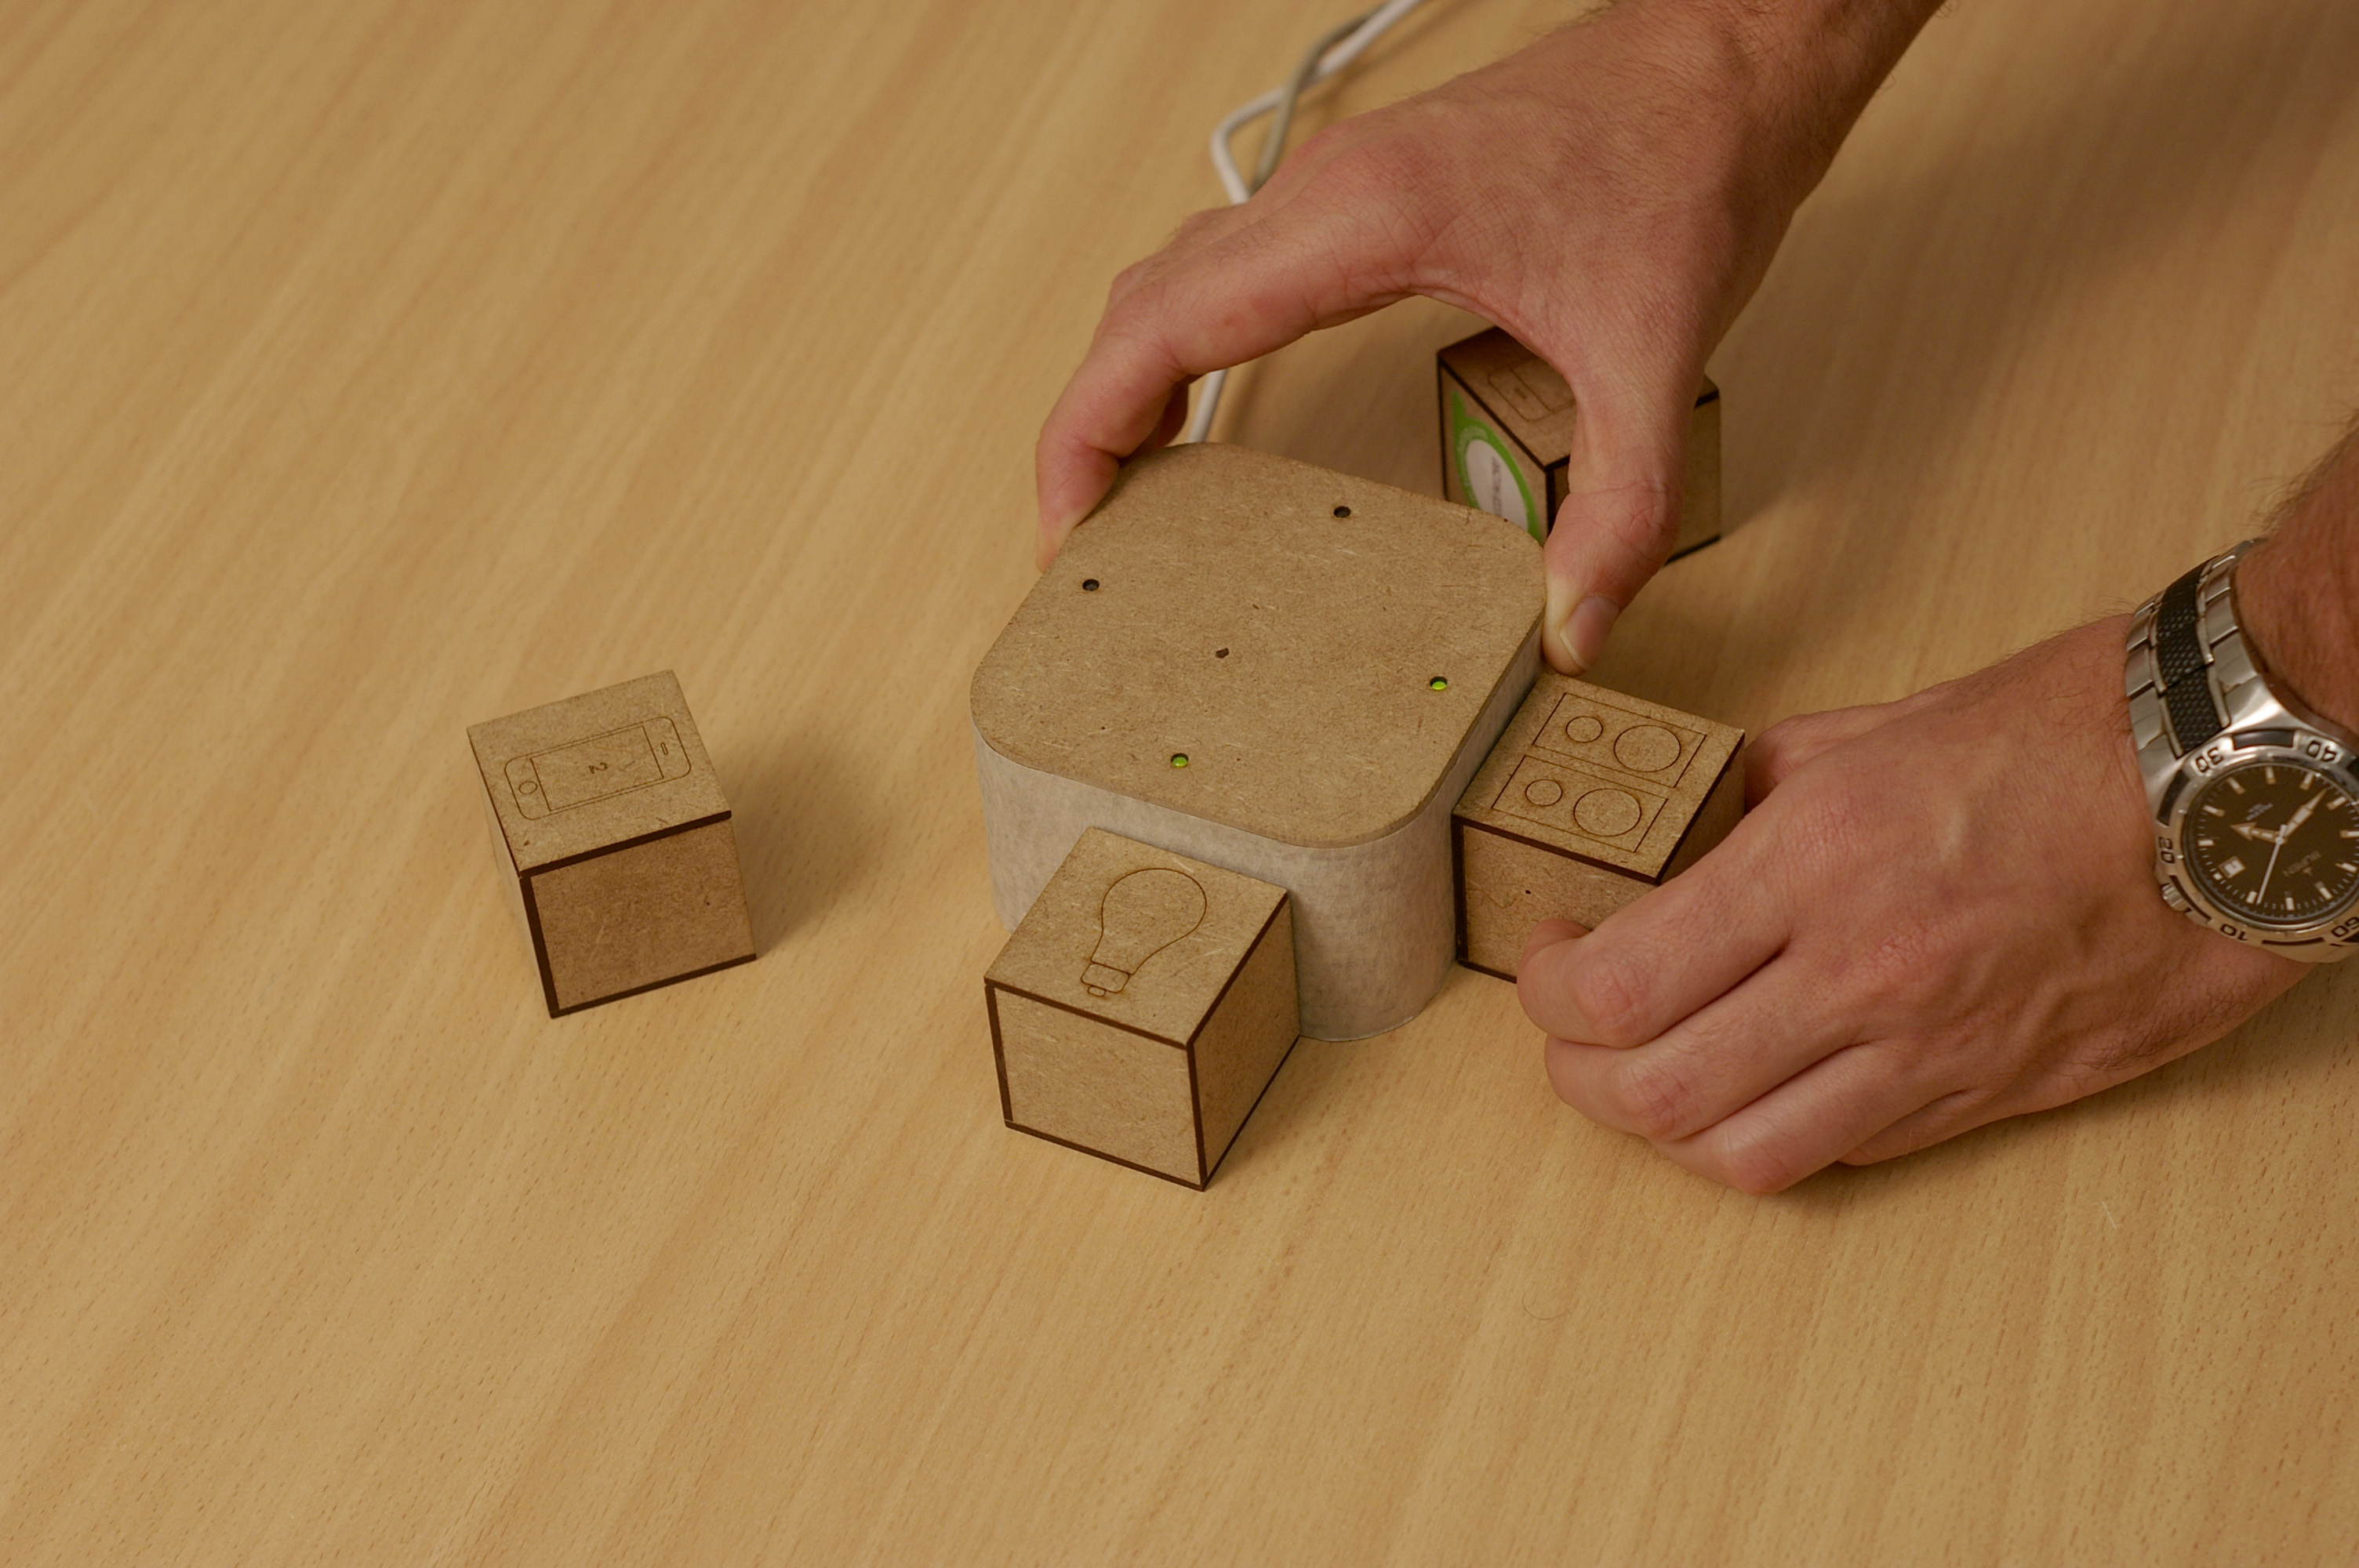
\includegraphics[width=260pt]{tile2}
\caption{A laser-cut version of the interaction tile prototype}
\label{tile2}
\end{figure}

Two alternative designs are presented in Van der Vlist's thesis \cite{Bram}. A more detailed discussion of the interaction tile and how its design is informed by product semantics is available in \cite{VanderVlist2010}. 

\subsection{Lamp}
\label{Lamp}
To create the ambient lighting system, we replaced the internals of a table lamp with an RGB LED array and an Arduino\footnote{ http://www.arkadian.eu/pages/219/arduino-controlled-ikea-lamp}. A Bluetooth module was connected to the Arduino to facilitate communication with a computer, the final result of which can be seen in Figure \ref{lamptile}.\marginpar{The Ikea Lampan lamp that was used for the prototype currently retails for around \euro 3.} 

\begin{figure}[bth]
\centering
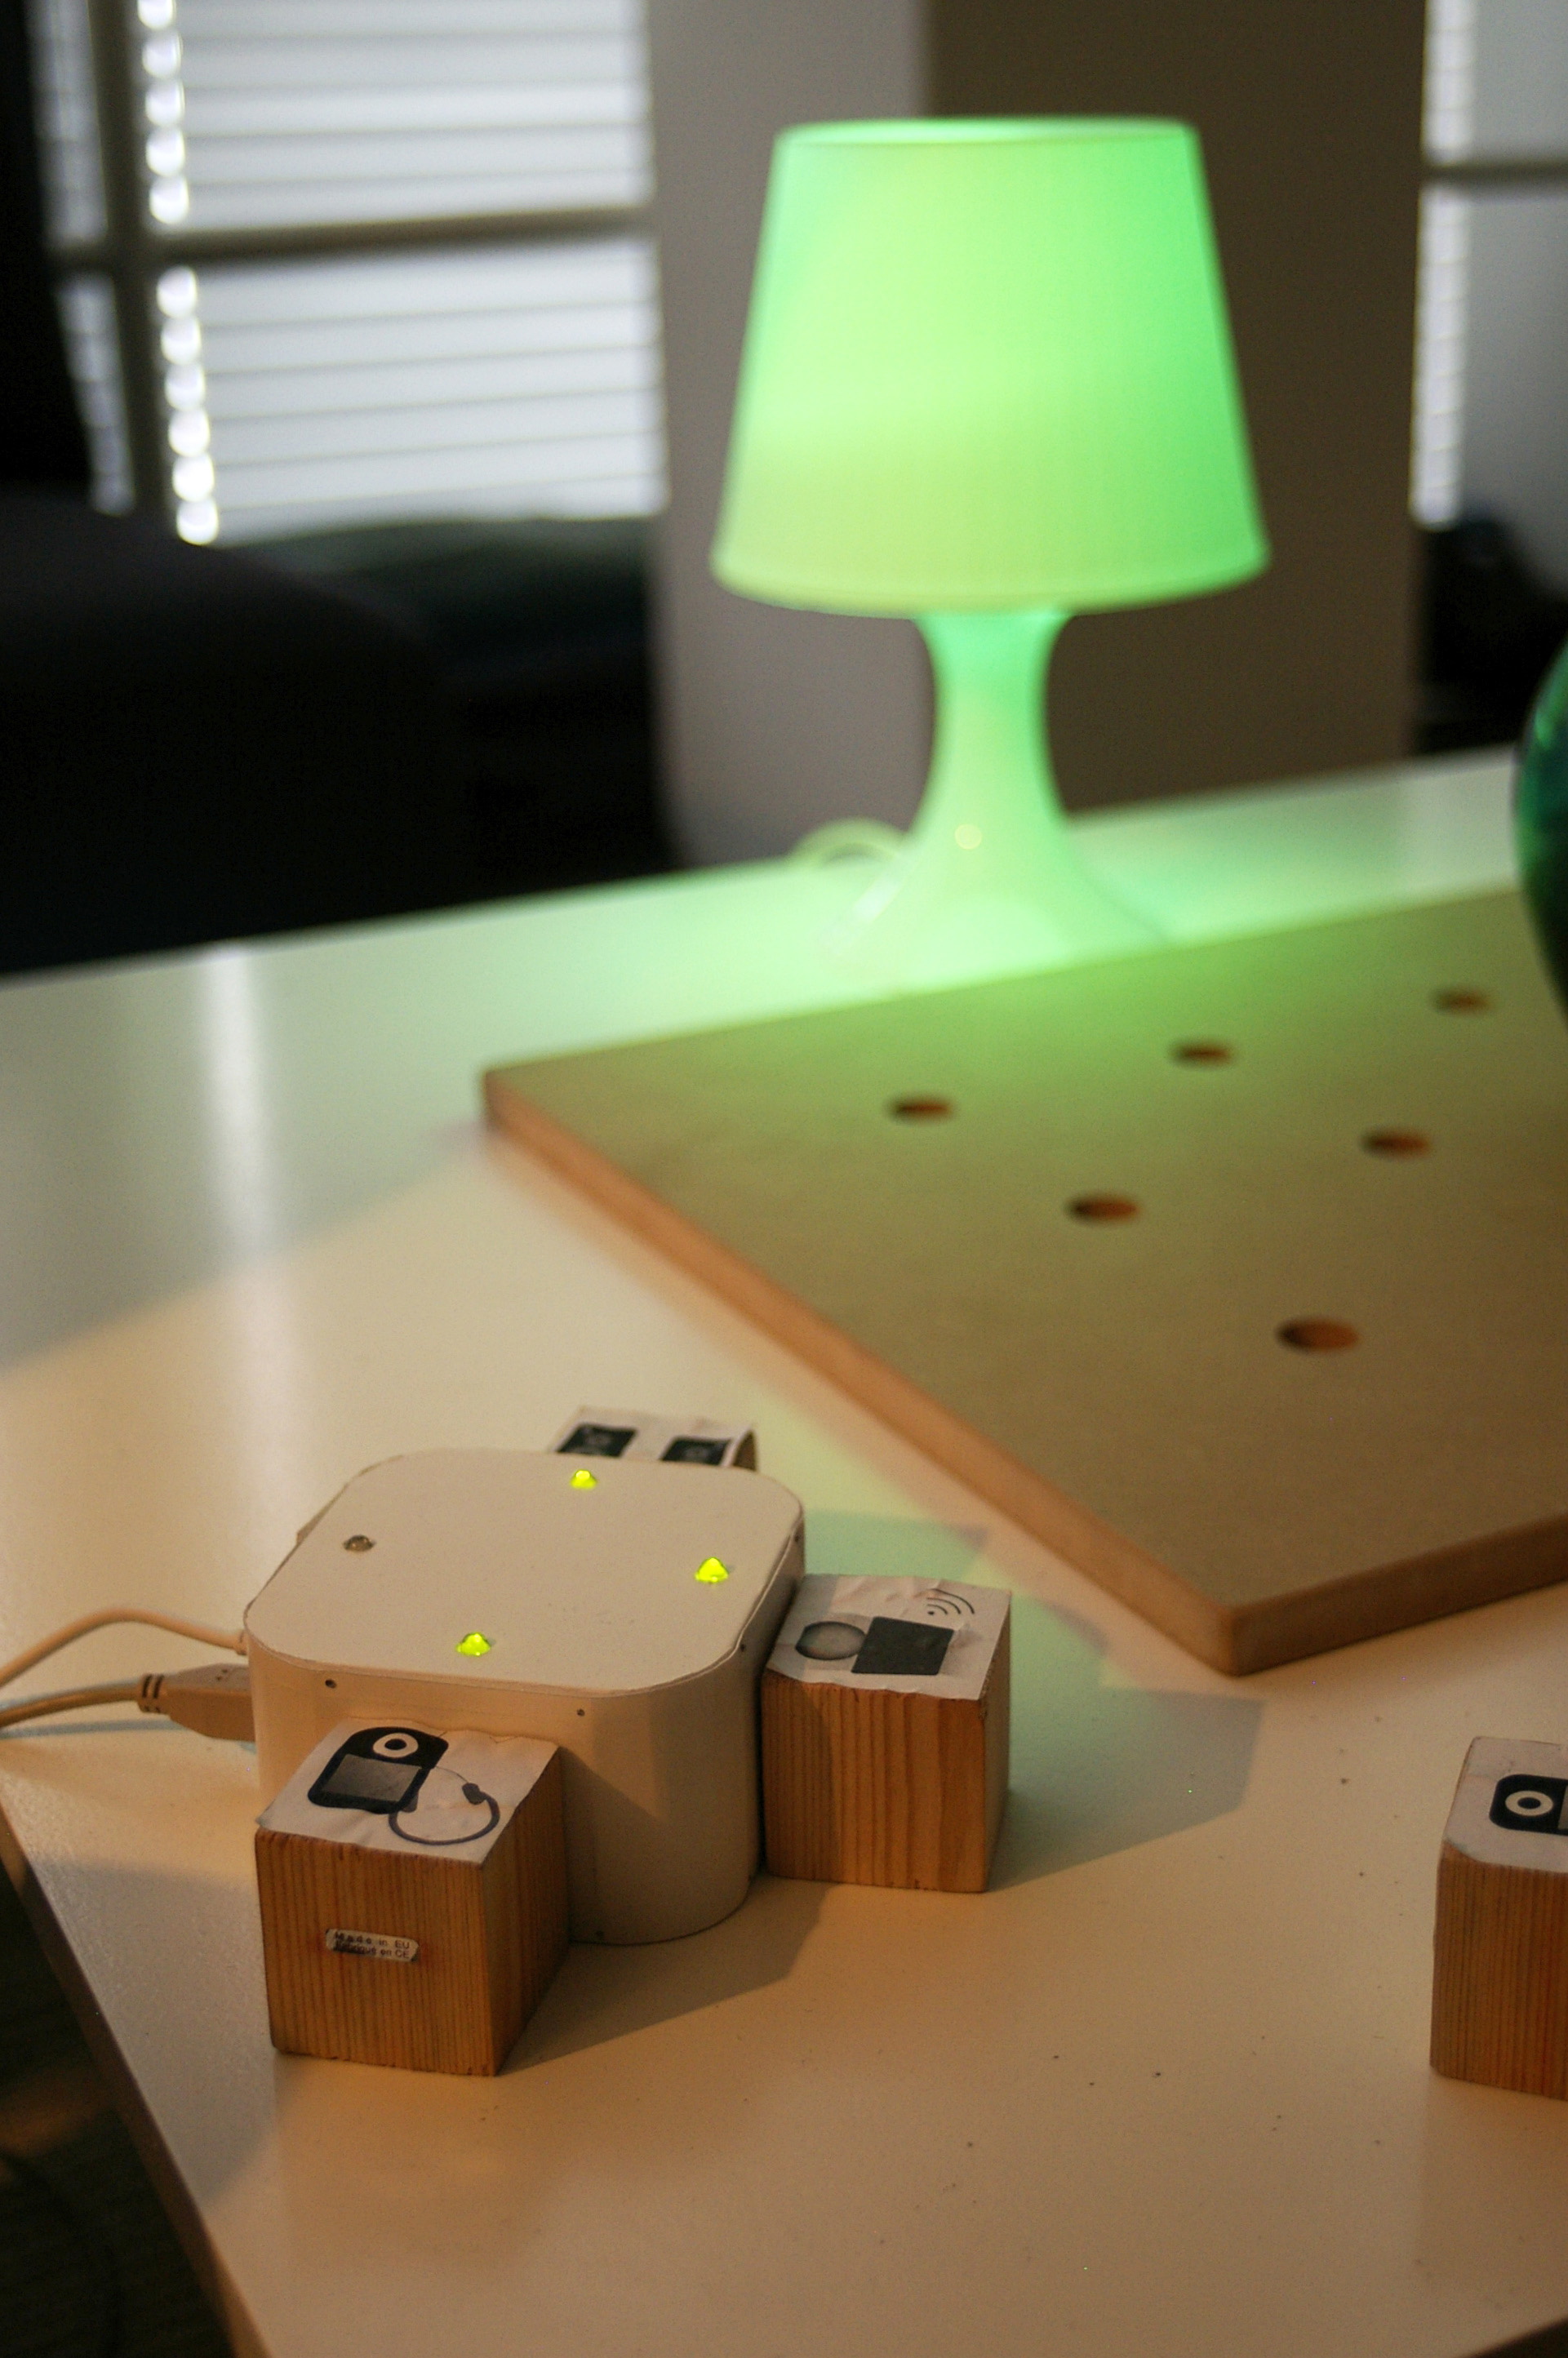
\includegraphics[width=260pt]{lamptile}
\caption{The interaction and cubes, with the lamp in the background}
\label{lamptile}
\end{figure}

The coloured lighting can be changed by sending three RGB values (in the range 0-255) to the lamp via the serial-over-Bluetooth interface.

\subsection{Mobile phones}

For the first iteration, a Nokia N95 and Nokia 5800 XpressMusic phone (shown in Figure \ref{lampphone}) were used. The two phones use the Symbian S60 operating system, and Python for S60 was used to write software for the mobile phones.\marginpar{Python for S60 is Nokia's port of the Python programming language for Symbian devices.}

\begin{figure}[bth]
\centering
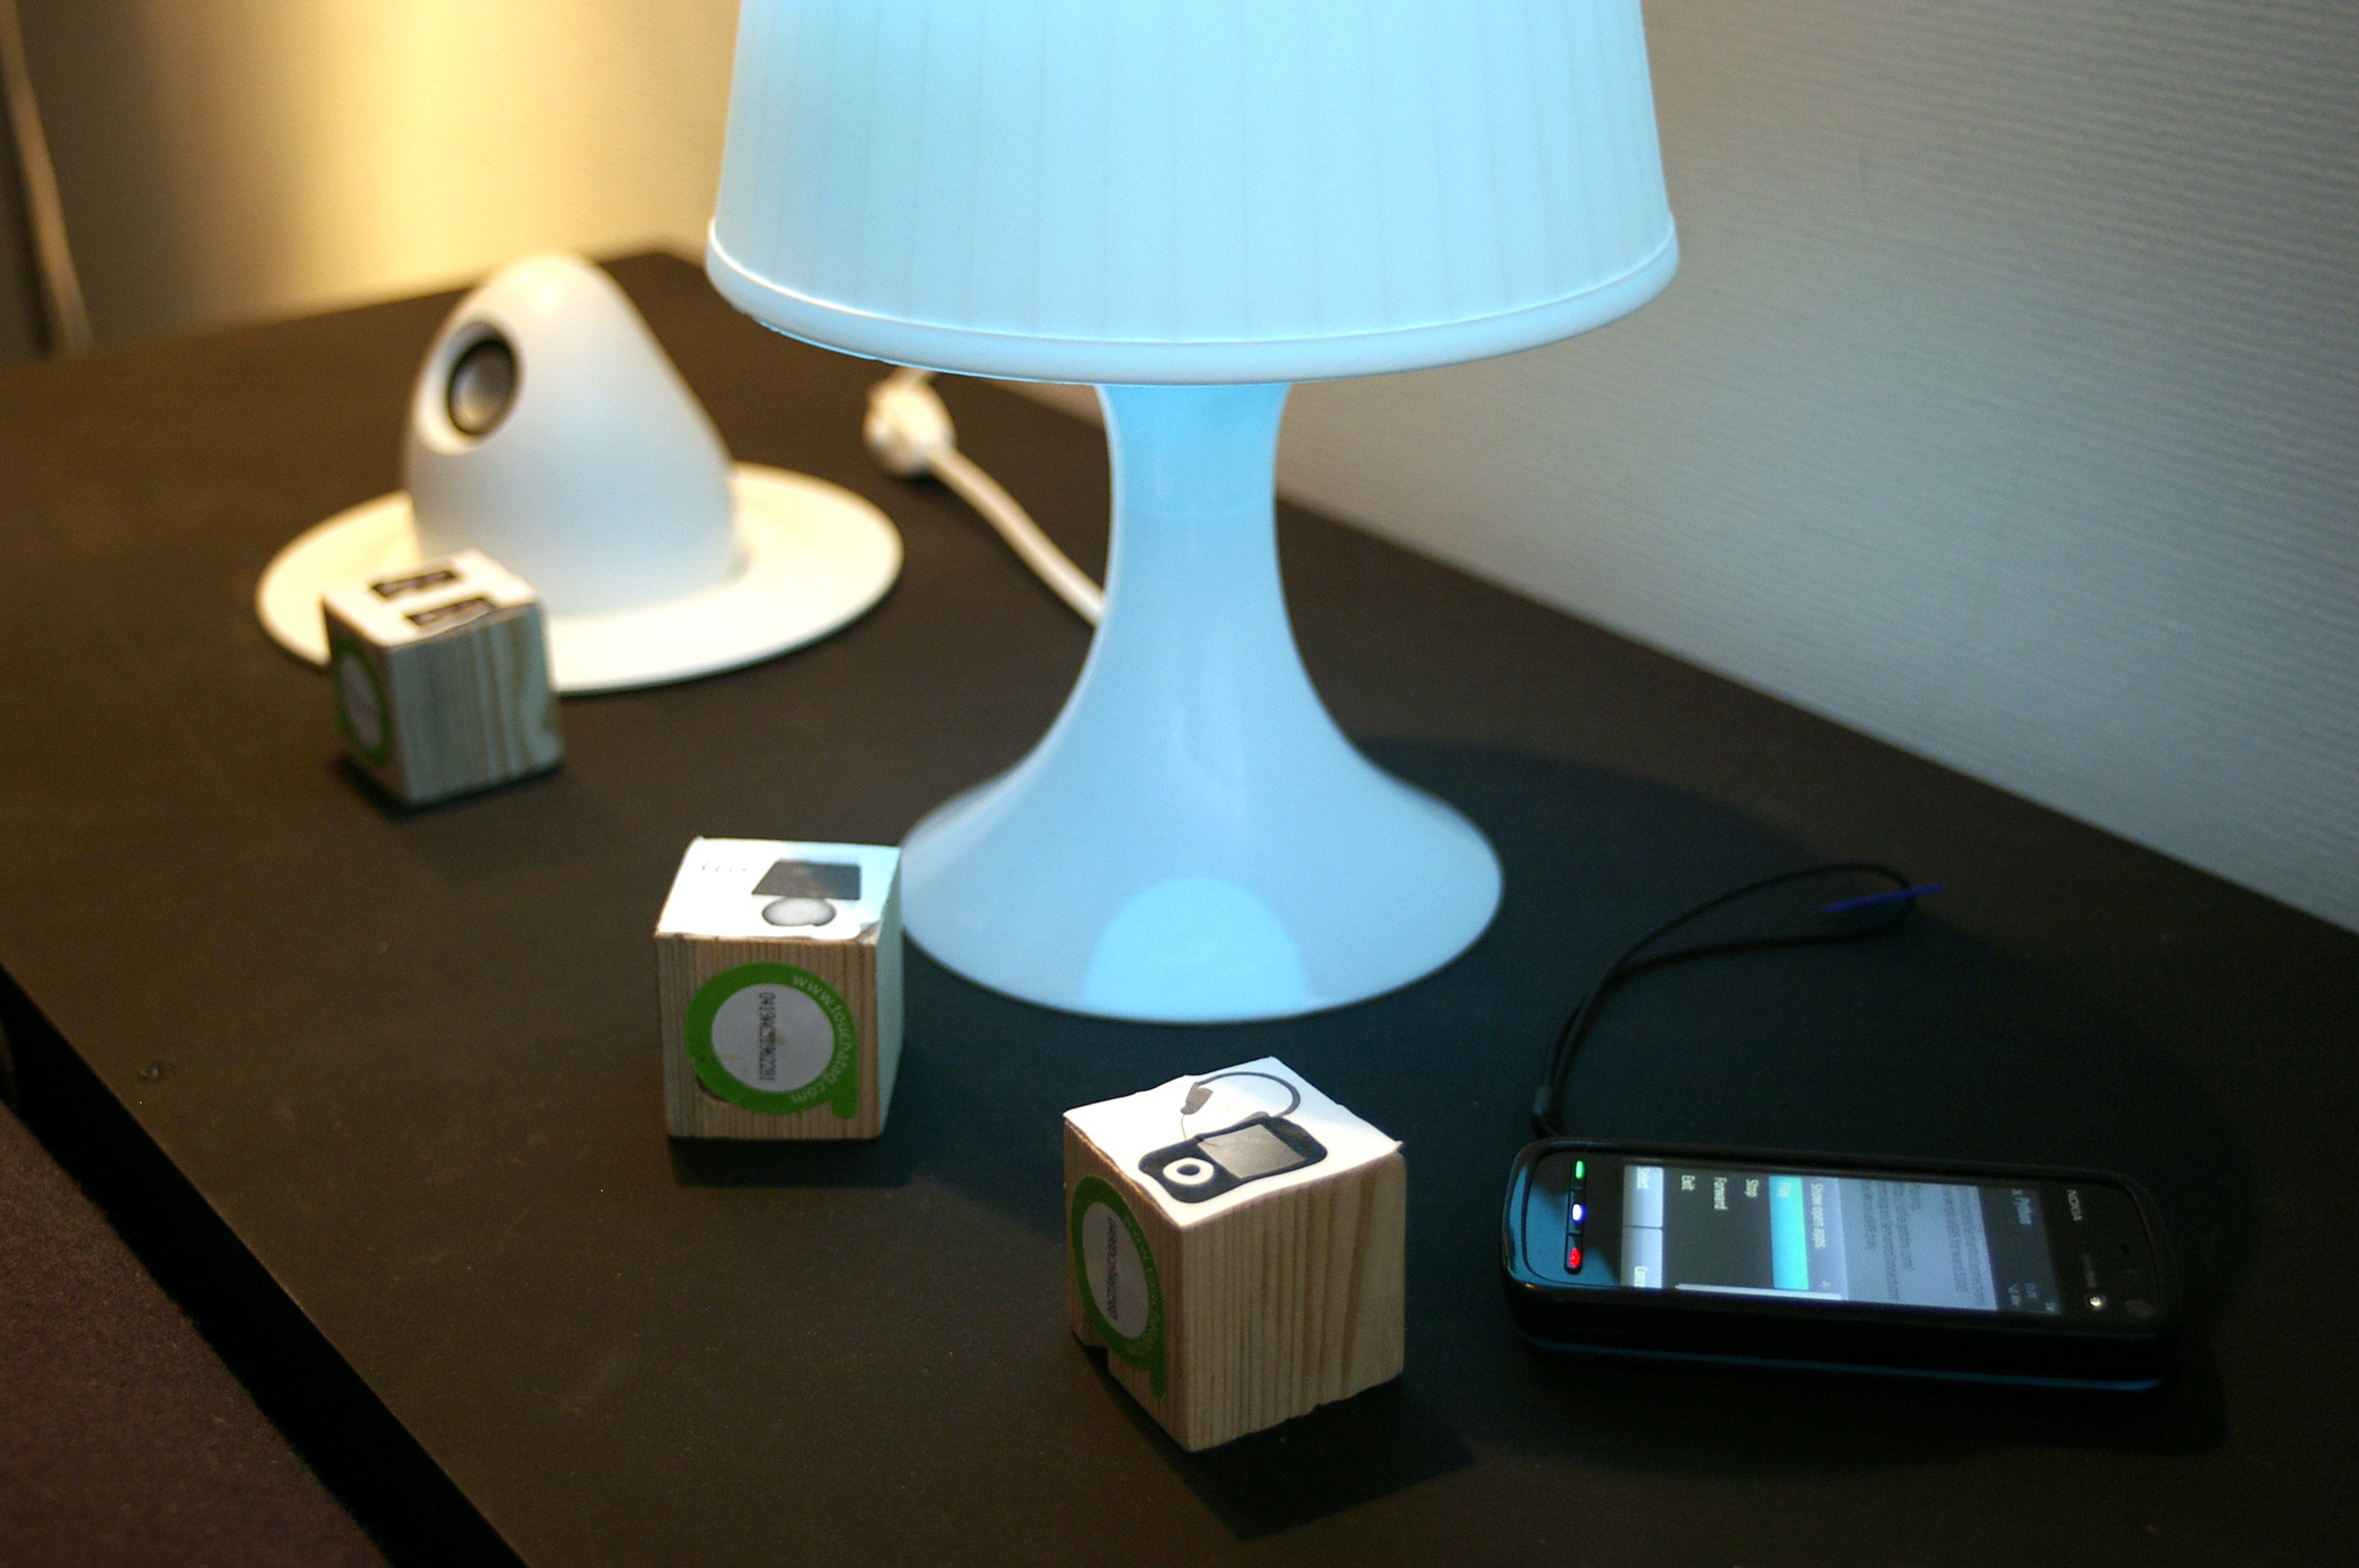
\includegraphics[width=260pt]{lampphone}
\caption{The Nokia 5800 XpressMusic mobile phone with the lamp and some cubes}
\label{lampphone}
\end{figure}

\subsection{RFID reader used in interaction tile}

Most of the \ac{RFID} readers and tags targeted at the amateur and hobbyist markets, like the PhidgetRFID and Innovations ID-12 modules, operate in the 125KHz range. While they are relatively cheap and readily available, the 125KHz readers cannot read multiple tags within range of the reader at the same time. For this a 13.56MHz reader is required. The most widely used \ac{RFID} tags at the moment, the MiFare range owned by NXP, operate at 13.56MHz. These tags are used in most public transport payment systems, including the London Oyster Card and the Dutch OV-Chipkaart system.

A relatively cheap 13.56MHz \ac{RFID} reader system, the ACR122, is developed by Hong Kong-based \ac{ACS}. It uses the NXP PN532 chip to read \ac{RFID} tags. \marginpar{A rebranded version of the ACR122, called the Touchatag\footnote{http://www.touchatag.com/}, is currently sold with 10 tags for around \euro 30.} The reader has an onboard PCB antenna -- to extend the range of the unit we removed two capacitors on the PCB and soldered in an external ANT-1356M coil antenna from RF Solutions.
%- Hacking the Touchatag (\euro 33) by adding our own external antenna (see circuit diagram)



\section{Implementation}
\label{D1Implementation}
\begin{figure}[bth]
\centering
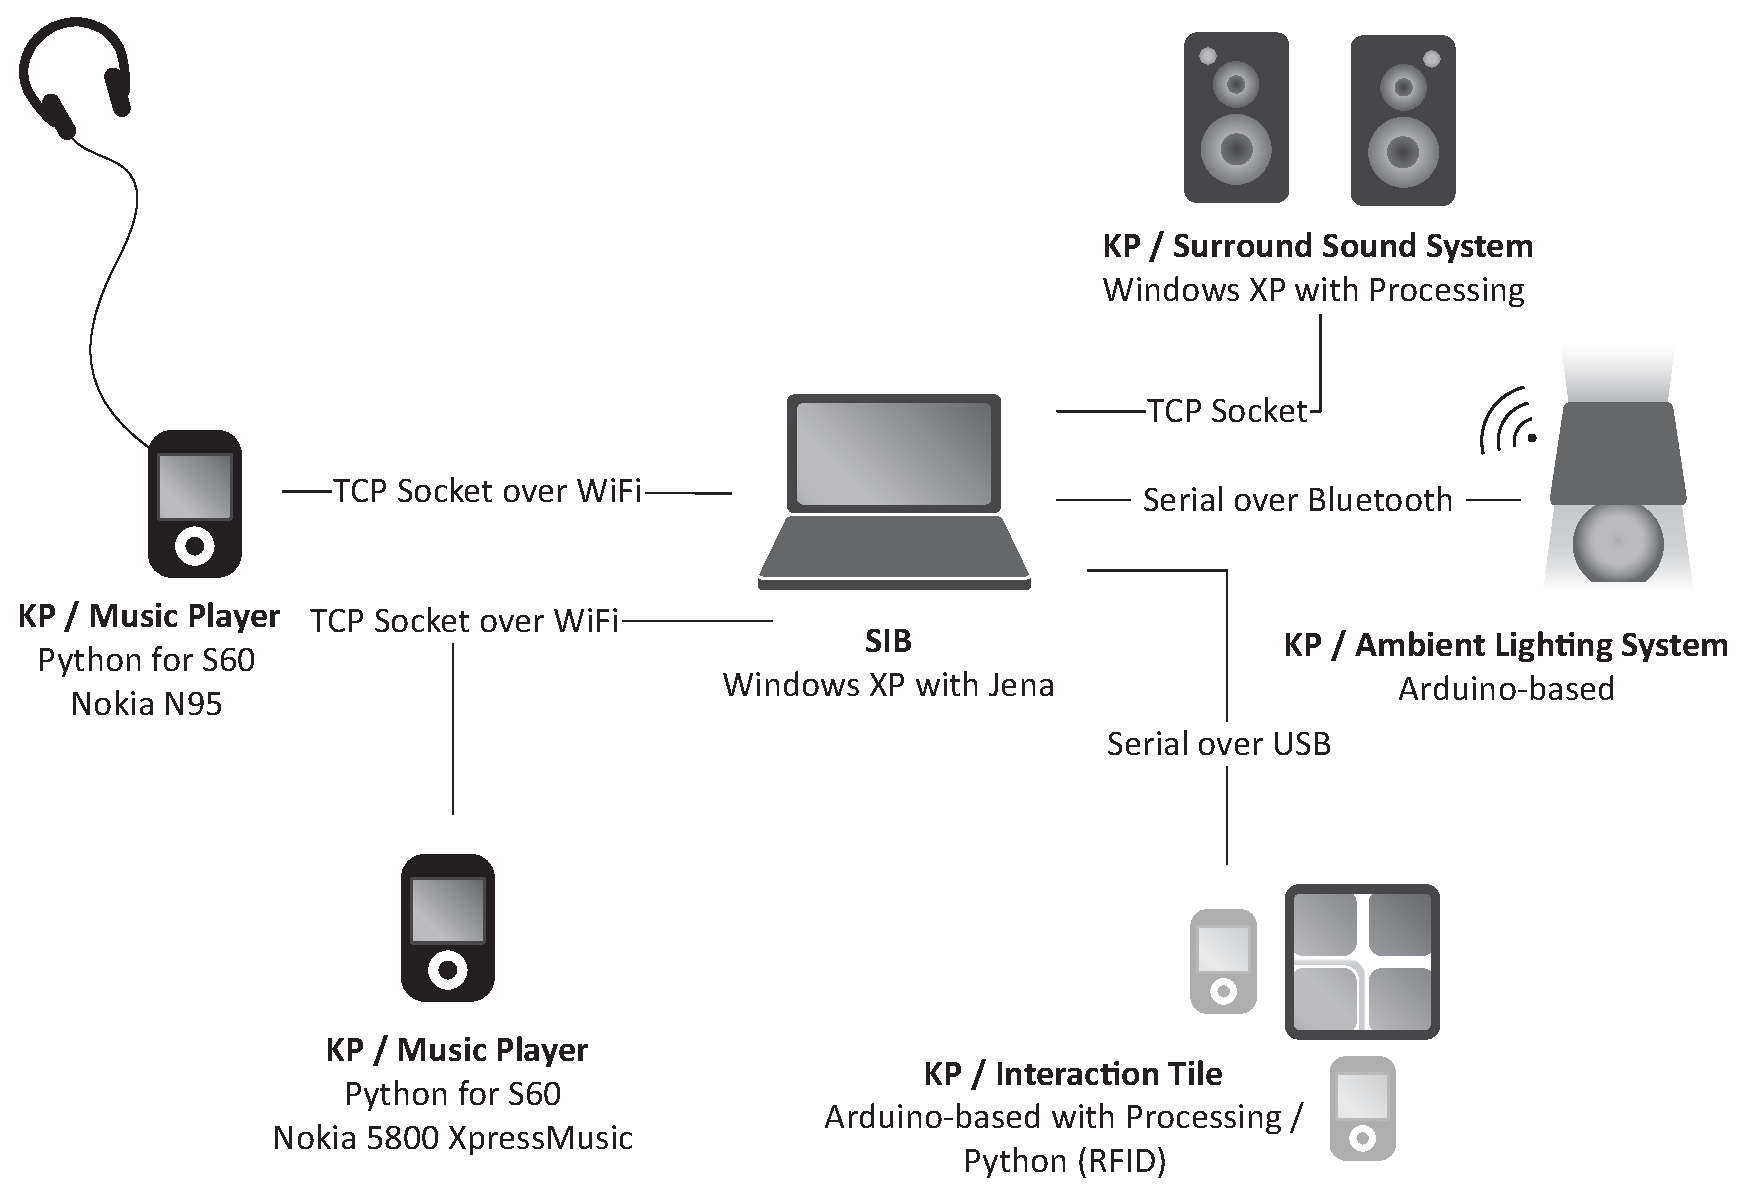
\includegraphics[width=360pt]{SemanticConnections.eps}
\caption{An overview of the demonstrator}
\label{semanticConnections}
\end{figure}

Following the design and development of the ontology and required devices, a demonstrator that implements the the scenario was created. A visual overview of the demonstrator can be seen in Figure \ref{semanticConnections}. A video of the scenario is available\footnote{https://vimeo.com/15594590}.

\begin{figure}[bth]
\centering
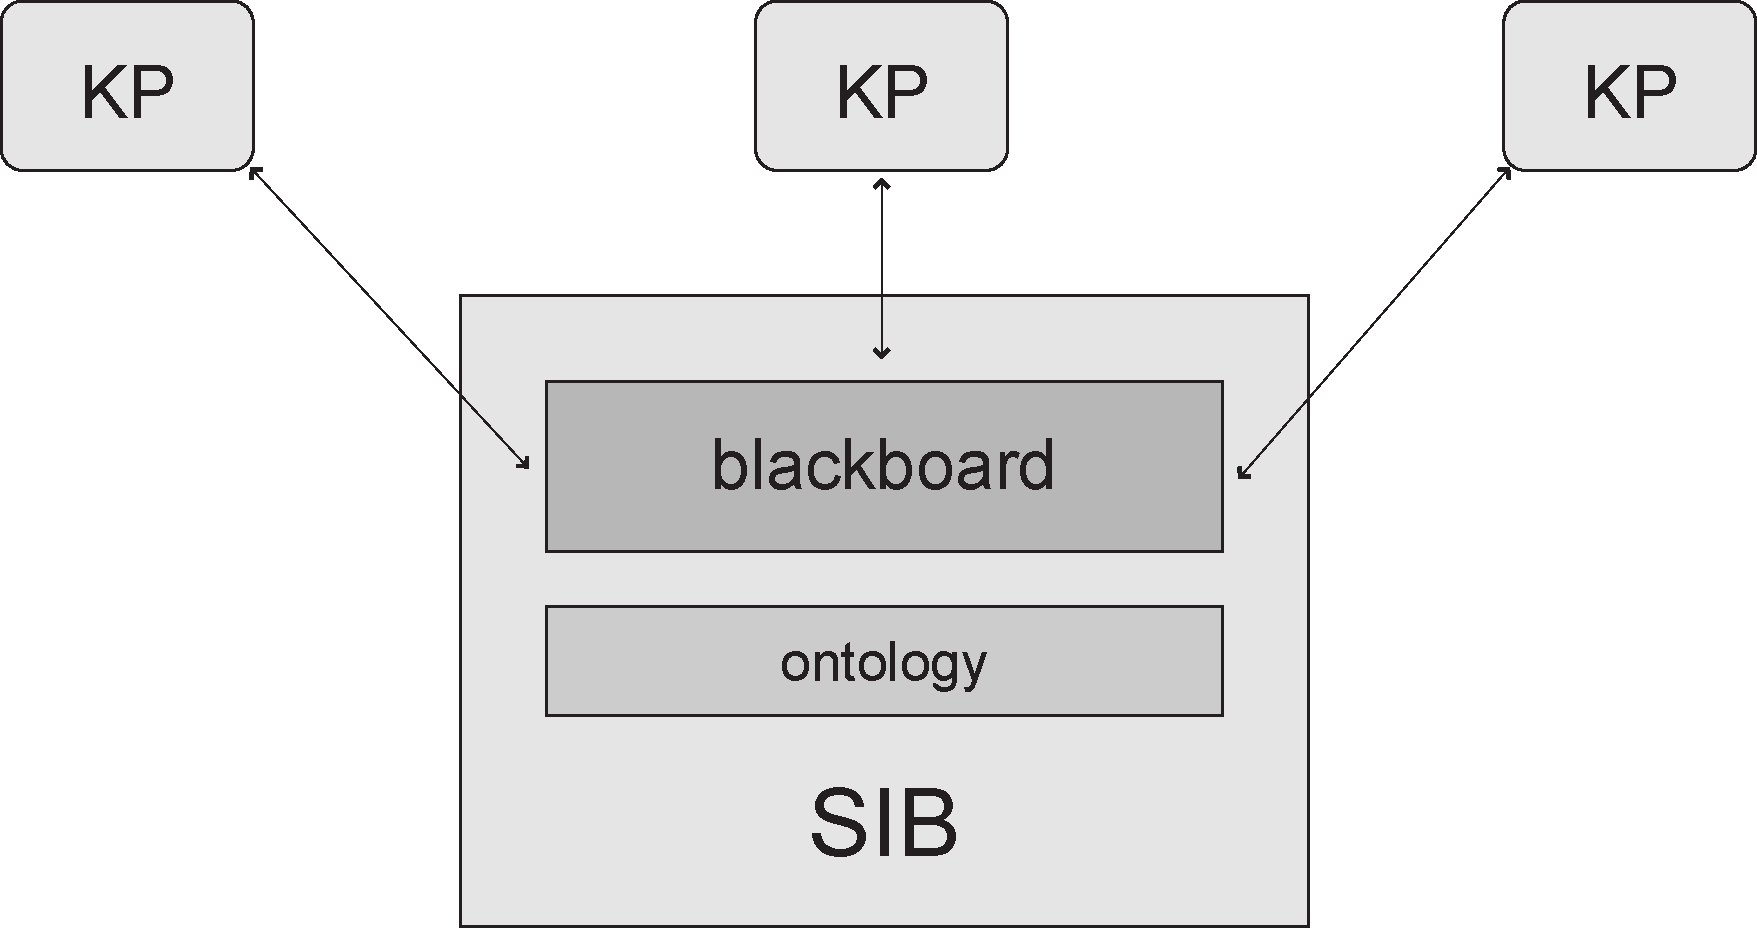
\includegraphics[width=260pt]{blackboard}
\caption{System architecture of demonstrator}
\label{blackboardarch}
\end{figure}

Each device in the demonstrator is represented by a \ac{KP} software module. \acp{KP} communicate via the \ac{SIB}, as shown in Figure \ref{blackboardarch}. As discussed in Section \ref{sofia}, the \ac{SIB} acts as an information broker, distributing messages between devices. This was an early design decision to reduce coupling, by minimising direct communication between devices, with all messages relayed via the \ac{SIB}. This philosophy of having a blackboard architectural model, where devices can write to and read from, was followed through all subsequent design iterations. The technical implementation of the various \acp{KP} are described in the following subsections.\marginpar{The system architecture model is described in more detail in Chapter \ref{SoftwareArchitecture}.}


\subsection{Interaction Tile KP}

The interaction tile \ac{KP} was written in Python and tested on Ubuntu Linux 10.04. On startup, the \ac{KP} connects to the Arduino inside the interaction tile via the serial-over-USB interface. It establishes a connection with the \ac{SIB}, after which it connects to the \ac{RFID} reader inside the tile.\marginpar{The open-source rfidiot.org library was used to communicate with the \ac{RFID} reader.}

The \ac{KP} then enters an event loop, waiting until a cube is placed next to the tile. When this happens, the Arduino sends the position of the cube next to the tile to the \ac{KP} via the serial interface. The \ac{RFID} tag is read, and a \texttt{NFCEnterEvent} is generated. After the \ac{RFID} tag is read it is temporarily disabled, to ensure that the tag will only be read again after being removed from the field and coming into range again.

If the tile is shaken and a connection is possible, the \ac{KP} updates the \ac{SIB} by inserting \texttt{connectedTo} relationships between the devices, represented by the cubes next to the tile. If there are existing connections, the \texttt{connectedTo} relationships are removed instead. When a cube is removed from the tile, the Arduino again sends the position of the cube via the serial interface to notify the \ac{KP}. The \texttt{python-pyscard}, \texttt{pcsc-tools} and \texttt{pcscd} \ac{PC/SC} libraries are required on Ubuntu Linux to communicate with the \ac{RFID} reader.

\subsection{Music Player KP}
\label{MusicPlayerKP}
This Python-based \ac{KP} runs on Symbian S60. It has been tested on a Nokia N95 and Nokia 5800 XpressMusic phone. When the \ac{KP} starts up, it connects to the \ac{SIB}, generates a \texttt{ConnectEvent} and subscribes to new \texttt{PlayEvent}s, \texttt{StopEvent}s and \texttt{CueEvent}s. It then enters an event loop. Pressing the play/stop/forward buttons on the phone's \ac{GUI} will generate the corresponding event, and the \ac{KP} will also respond to events generated by other devices that it is connected to via the \texttt{connectedTo} relationship.

Another version of the music player \ac{KP} was developed for a Nokia N900 smartphone that runs on Maemo 5 Linux. This \ac{KP} was also written in Python and makes use of the PyQt4 library. This \ac{KP} is functionally equivalent to the Symbian S60 version, apart from running on the Maemo platform and using the Qt4 Phonon framework to provide music play/stop/forward capabilities.
% - N900 - used pyside and QtMobility (24/08/10)

\subsection{Light KP}

This \ac{KP} was written in Java and makes use of the Minim audio library\footnote{http://code.compartmental.net/tools/minim/} for beat detection, in order to generate meaningful lighting patterns that can be sent to the table lamp.\marginpar{The Minim audio library is part of the Processing software development environment, used for interaction design prototyping.}

The \ac{KP} listens for media player events from connected devices, and generates RGB values based on the rhythm of the music. These RGB values are then sent to the Arduino in the table lamp via the serial-over-Bluetooth interface. On Ubuntu Linux the \texttt{librxtx-java} package is required for serial communication when using Java.

Part of the event handler that handles subscriptions from the \ac{SIB} is shown in the following code fragment:

\begin{minted}{java}
@Override
public void kpic_SIBEventHandler(String xml) {
String subject = null;
String object = null;
String predicate = null;

println("Subscription notification!");
//Get triples that were added or updated in the SIB
Vector<Vector<String>> triples = 
		xmlTools.getNewResultEventTriple(xml);

if(triples!=null){
  for(int i=0; i<triples.size() ; i++ ){ 
	Vector<String> t=triples.get(i);
	subject=xmlTools.triple_getSubject(t);
	predicate=xmlTools.triple_getPredicate(t);
	object=xmlTools.triple_getObject(t);

	// when we have a new connectedTo 
	// relationship to the LightKP
	if(predicate.contains("connectedTo") && 
			object.contains(deviceID)){

		//subscribe to source events
		subscribeToSourceEvents(subject);
  }
  ...	
\end{minted}

When the Light \ac{KP} is connected to another device \ac{KP} using a \texttt{connectedTo} relationship, we subscribe to the interaction events generated by that device using the \texttt{subscribeToSourceEvents()} function. This code fragment is shown below as an example of how subscriptions are created using the Java \ac{KP} interface:

\begin{minted}{java}
void subscribeToSourceEvents(String source) {

println("Subscribing to source events from " + source); 
xml=kp.subscribeRDF( null , sofia + "launchedBy" , source, URI);

if(xml==null || xml.length()==0){
print("Subscription message NOT valid!\n"); return;}
print("Subscribe confirmed:"+
(this.xmlTools.isSubscriptionConfirmed(xml)?"YES":"NO")+"\n");

if(!this.xmlTools.isSubscriptionConfirmed(xml)){return;}
String sub_id = this.xmlTools.getSubscriptionID(xml);
println("Subscription ID: " +sub_id);
subscriptions.put(source,sub_id);
}	
\end{minted}


%- Use ~/code/semanticconnections/docs to describe technical implementation 
%	- C-based SIB (Piglet triple store, with component requirements 19/05/10 - to appendix?)
%	- dependencies (06/09/10)

\subsection{SIB}
%- Components required are (18/05/10 Notebook1)

The first \ac{SIB} implementation used in the \ac{SOFIA} project is called Smart-M3, developed by Nokia, and an open source implementation is available online\footnote{http://sourceforge.net/projects/smart-m3/}. The \ac{SIB} is written in C and uses Nokia's Piglet triple store as a database backend. It is only available on Linux as it makes of the D-Bus message bus system. Other dependencies include the Avahi service discovery framework and Expat XML parser.  The \ac{SIB} consists of a daemon called \texttt{sibd}, which communicates with \acp{KP} over TCP/IP using a \texttt{sib-tcp} connector module.  



\section{Discussion \& Conclusion}

%- Proximal interactions with tangible interfaces
%- First use of Smart-M3
%- Triple-format queries from KP e.g. None,ie:hasRFIDTag,None (Evaluate against SPARQL queries from KP?)
%- Input: Interaction events (multimodal fusion) and implicit interaction (sensor observations) (discussed in TiiS paper)



This first iteration constructed a number of devices that could be reused in future iterations, and explored approaches to creating connections between devices. These approaches were focused at proximal interactions with tangible interfaces instead of the usual \ac{GUI}-based solutions. Let us look at some issues that were uncovered during the implementation, followed by a conclusion. 

This iteration details the first use of Smart-M3, where \acp{KP} communicate with a \ac{SIB} using \ac{SSAP}\cite{Honkola2010}. \ac{SSAP} consists of a number of operations to insert, update and subscribe to information in the SIB. These operations are encoded using XML. A triple-format query from a \ac{KP} is sent, and the response from the \ac{SIB} is in triple-format as well. %An example of a triple-format query is \mint{turtle}|None hasRFIDTag None| where \texttt{None} is used to denote the wildcards in the query. The response to this query would be a list of triples containing smart objects and their associated \ac{RFID} tags.

We attempt to solve the interoperability problem by following a blackboard-based approach. Some of the problems associated with current blackboard-based platforms are scalability and access rights. While the goals of this thesis do not involve solving these problems, they should be considered as possible constraints. In Chapter \ref{Evaluation} we will look in more detail at the performance-related issues of the system architecture. 

The evaluation of this iteration, where the various alternative tangible approaches are compared in a usability study, is discussed in more detail in \cite{Kwak2011}. This study was performed in the Context Lab at the Eindhoven University of Technology, and made use of the Teach-Back protocol \cite{VanDerVeer2003} and Norman's Action Cycle Diagram \cite{Norman1998}.

From this first iteration we learned that using interaction events to model device and user interaction works well. Yet the different types of interaction events need to be generalised, so that they can be reused in other scenarios and environments. One difficulty we encountered was how to model the capabilities of devices in more detail so that they can be shared with other devices. In the next chapter we extend the scenario to include devices from our various partners in the \ac{SOFIA} project, and model the media capabilities of devices in order to perform semantic matching of different media types.  



%(already in intro)
% We consider context awareness to be one of the most important features of a smart environment, especially when we consider a user's interaction with the smart space. Considering the parallel nature of our interaction with the physical world, any smart space will require context to help it make sense of the many different ways in which users map their tasks onto the environment.
% 
% Where the system tries to predict what the user is trying to accomplish, by being adaptive and anticipatory, we need to identify ways to give the users appropriate means to express themselves. The possibilities, available services and information that exist in the smart environment needs to be communicated in a meaningful way. Only if this is done correctly will users be able to build helpful mental models of the functionality the environment has to offer, set goals and make plans on how to act. By developing novel and meaningful interaction devices, the user can then perform the necessary actions and the system can in turn try to understand the user's goals and make the match to its internal models. We see a vital role here for the theory of \emph{product semantics} \cite{feijs-commutative}, the study of how artefacts acquire their meaning and use its theories to define common concepts and semantics. 

%To be able to create a personalized environment, we consider both runtime task models and the BDI model to be important. Task models may be used to describe the user's actions, while the BDI model may be used to represent the psychological, social and situational aspects of the tasks. Once the task model is defined, the system can adapt to the user, by mapping the user's current activity or task to higher-level goals and intentions.

%The BDI model approach focuses on the anticipatory aspect of ambient intelligence, where the system tries to predict what the user is trying to accomplish. We also hope to use the low-level events and command currently implemented in the system to automatically infer higher-level tasks and goals, with the final step being able to model the user's (and/or agent's) intentions using an ontology.

%end SISS2010
\chapter{Design iteration II}
\label{DesignIteration2}
\begin{flushright}{\slshape    
If interaction design is considered only at the end, \\
software is driven by engineering design, of which \\
users are rightly unaware, rather than by representations \\
with which they interact.} \\ \medskip
    --- Gillian Crampton Smith and Philip Tabor \cite{Winograd1996}
\end{flushright}

\marginpar{Parts of this chapter appear in \cite{Niezen2011}, \cite{Vlist2011} and \cite{VanderVlist2012a}.}

The second iteration was driven by a collaboration with various partners in the \ac{SOFIA} project, which included Philips, NXP, Conante and the TU/e \ac{SAN} research group . This collaboration culminated in a joint demonstrator that was exhibited and evaluated at the Experience Lab at the High Tech Campus in Eindhoven --- the Smart Home pilot.

\section{Requirements}
\label{D2Requirements}
%- Should allow for actively or automatically manipulable instances (Semantic transformers?) \cite{Mitsui08}

The Smart Home pilot is based on the following scenario:

\textit{Mark and Dries enter their home. A presence sensor detects their presence and notifies the smart space. The decorative wall-wash lights are in turn notified of user presence by the smart space, and turn themselves on. Mark and Dries start listening to music. They would like to try to render the music on a lighting device to also create some visual effects accompanying the music. They query the smart space and find out that the lighting device can render these light effects. They make a connection between the music player and the lighting device using the Connector. The light starts being rendered on the lighting device. To put the focus on the lighting device, the decorative wall-wash lights in the room automatically dim themselves down. At the same time, the light pattern also starts being rendered on the remote lighting device, where Mark's sister Sofia can observe the same light effects in her own house.}

\textit{At another location: Sofia enters her house and the intelligent lighting system detects her presence, notifies the smart space and switches the lights on. After a while, Sofia is curious and wants to listen to the music that Mark and Dries are listening to. She connects her lighting device to her stereo using Spotlight Navigation, and the same song plays on her surround sound system.}

There are some obvious similarities with the previous scenario in Chapter \ref{DesignIteration1}. However, there are a number of additional devices introduced:

\begin{itemize}
	\item Presence sensor and wall-wash lighting - A system developed by TU/e \ac{SAN} that detects the user's presence and switches the lights on automatically
	\item Lighting device - An ambient lamp developed by Philips, based on their LivingColors technology
	\item Intelligent lighting system - A lighting system developed by NXP that also detects the presence of users
	\item Spotlight Navigation - An augmented reality approach to exploring semantic connections, based on technology developed by Conante
\end{itemize}

We first focus on the design of the ontologies that were created to support these kind of scenarios, followed by the design of the devices that were created specifically for the pilot.


\section{Ontology Design}
\label{OntologyDesign2}

The \emph{Semantic Media} ontology and \emph{Semantic Interaction} ontology were created during Iteration II to enable interoperability between the devices of the different partners involved in the Smart Home pilot.

\subsection{Semantic Media ontology}
\label{SemanticMediaOntology}

%begin S3E
% \begin{figure}
% \centering
% 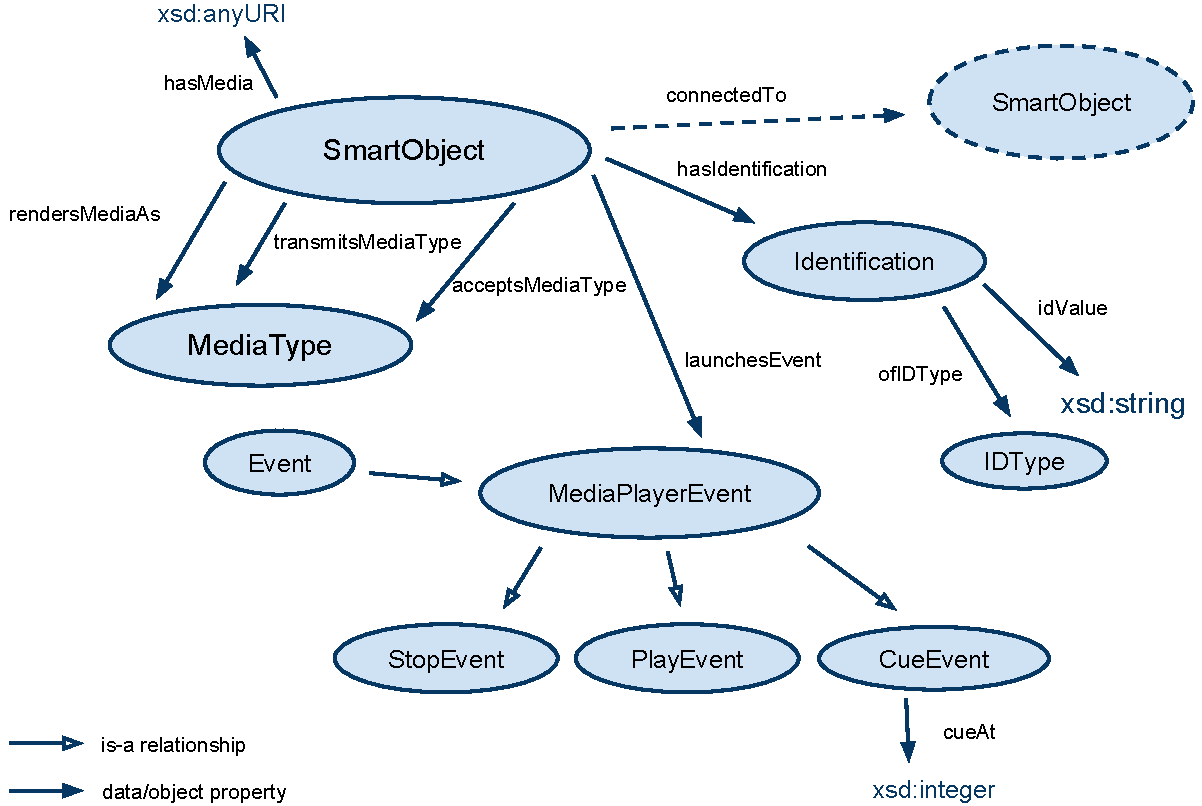
\includegraphics[width=300px]{SemanticMediaOntology}
% \caption{Semantic Media Ontology}
% \label{semanticMediaOntology}
% \end{figure}


\begin{figure}[bth]
	\digraph[scale=0.45]{ontologyInstance}{
		rankdir=LR;
		%node[shape="box"];
		anyURI [label="xsd:anyURI", shape="plaintext"];
		integer [label="xsd:integer", shape="plaintext"];
		datetime [label="xsd:datetime", shape="plaintext"];
		SmartObject -> MediaPlayerEvent [label="launchesEvent"];
		SmartObject -> MediaType [label="rendersMediaAs"];
		SmartObject -> MediaType [label="transmitsMediaType"];
		SmartObject -> MediaType [label="acceptsMediaType"];
		SmartObject -> anyURI [label="hasMedia"];
		MediaPlayerEvent -> StopEvent [style="dotted"];
		MediaPlayerEvent -> PlayEvent [style="dotted"];
		MediaPlayerEvent -> CueEvent [style="dotted"];
		CueEvent -> integer [label="cueAt"];
		Event -> MediaPlayerEvent [style="dotted"];
		Event -> datetime [label="inXSDDateTime"];
	}
	\caption{Semantic Media Ontology}
	\label{semanticMediaOntology}
\end{figure}\marginpar{The notation used for Figure \ref{semanticMediaOntology} was also used in Figure \ref{ontologyInstance} in Section \ref{OntologyDesign1}, where class membership is denoted with dotted lines and relationships are denoted with solid lines.}



The Semantic Media ontology, shown in Figure \ref{semanticMediaOntology}, is an application ontology that allows for describing media-specific device capabilities and related media content. A mobile device may be described as follows:


{\footnotesize
\begin{minted}{turtle}
MobileDevice rdf:type :SmartObject .
MobileDevice acceptsMediaType Audio .
MobileDevice transmitsMediaType Audio .
MobileDevice hasMedia "file://media/groove.mp3"^^xsd:anyURI .
MobileDevice rendersMediaAs Audio .
\end{minted}
}

The system configures itself through semantic reasoning based on these media type descriptions. \marginpar{An example of semantic reasoning with media type descriptions is described in Section \ref{D2Implementation}.} A media player event of type \texttt{PlayEvent}, that would be generated when the mobile device starts playing music, is described as follows:

{\footnotesize
\begin{minted}{turtle}
event1234-ABCD rdf:type PlayEvent .
event1234-ABCD inXSDDateTime "2001-10-26T21:32:52"^^xsd:dateTime .
MobileDevice launchesEvent event1234-ABCD .
\end{minted}
}

Smart objects may be connected to one another using the \texttt{connectedTo} relationship. When a device receives an event notification, it first verifies that it is currently connected to the device that generated the event, before responding to the event.

Smart objects may be connected to one another directly if there is a semantic match between transmitted and accepted media types. Otherwise a \emph{semantic transformer} will have to be be introduced to transform the shared content, while still preserving the actual meaning of the connection. \marginpar{An example of a semantic transformer is described in Section \ref{D2Implementation}.}

\begin{description}
	\item [Semantic transformer] A semantic transformer is defined as a service that transforms information shared between devices from one type to another, while preserving the meaning of the information.
\end{description}

The concept of a semantic transformers is considered an important part of the theory developed in this work, and its applicability to smart environments in general is discussed in Chapter \ref{SemanticConnectionsTheory}.



%begin africon
\subsection{Semantic Interaction ontology}
\label{sectionSemanticInteractionOntology}

% \begin{figure}
% \centering
% 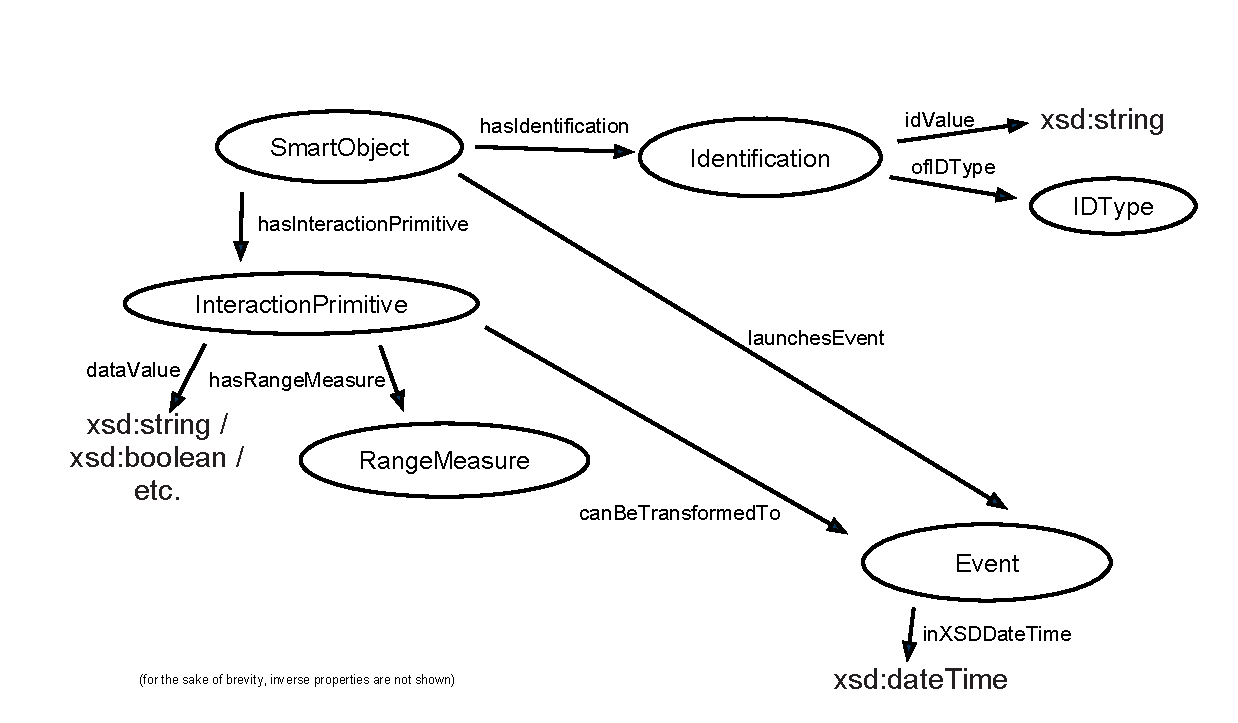
\includegraphics[width=350px]{SemanticInteractionOntology}
% \caption{Semantic Interaction Ontology}
% \label{semanticInteractionOntology}
% \end{figure} 


\begin{figure}[bth]
	\digraph[scale=0.45]{ontologyInstance2}{
		rankdir=LR;
		%node[shape="box"];
		etc [label="xsd:string / xsd:boolean / etc.", shape="plaintext"];
		string [label="xsd:string", shape="plaintext"];
		SmartObject -> InteractionPrimitive [label="hasInteractionPrimitive"];
		SmartObject -> Event [label="launchesEvent"];
		InteractionPrimitive -> etc [label="dataValue"];
		InteractionPrimitive -> RangeMeasure [label="hasRangeMeasure"];
		InteractionPrimitive -> Event [label="canBeTransformedTo"];
		SmartObject -> Identification [label="hasIdentification"];
		Identification -> string [label="idValue"];
		Identification -> IDType [label="ofIDType"];
	}
	\caption{Semantic Interaction Ontology}
	\label{semanticInteractionOntology}
\end{figure}


The Semantic Interaction ontology we have developed is shown in Figure \ref{semanticInteractionOntology}.  A device, defined as a \texttt{SmartObject}, is uniquely identified by some kind of \texttt{Identification}, for example a IP address and port number, \ac{RFID} tag or barcode. \marginpar{Identification is discussed in Section \ref{Identification}.} Different ID types can be defined as required. Devices can then launch events, for example a media player can generate a \texttt{PlayEvent} when music starts playing.


A smart object is described in terms of its \emph{interaction primitives}. \marginpar{The concept of interaction primitives is discussed in more detail in Section \ref{InteractionPrimitives}.}

\begin{description}
	\item [Interaction primitive]An \emph{interaction primitive} is defined to be the smallest addressable element that has a meaningful relation to the interaction itself. 
\end{description}

As an example of how the ontology may be used, we start off by defining a smart object and its interaction primitives. Recall that it is only necessary to describe interaction primitives of a device if we use that device's interaction primitive to control another device through the smart space. We can, for example, describe the volume control rocker switch on a smart phone as an interaction primitive:

\begin{minted}{turtle}
SmartPhone rdf:type SmartObject .
PhoneRockerSwitch rdf:type InteractionPrimitive .
SmartPhone hasInteractionPrimitive PhoneRockerSwitch .
\end{minted}

We now need to define the properties of the interaction primitive. We start by describing the range measure, or the range of values that the interaction primitive can produce (e.g. the rocker switch can produce \texttt{Up}, \texttt{Down} or \texttt{Neutral} values).

The range of values that an interaction primitive can take on is specified using a \texttt{RangeMeasure}. The list of range measures is shown in Table \ref{rangeMeasures}. These range measures are similar to the measure of the domain set used by MacKinlay et al \cite{MacKinlay1990}.\marginpar{MacKinlay's work was discussed in Section \ref{interactionTasks}.} Using the range measures, we can then infer which transformations may be used to map the input values to other interaction primitives or events. The ontology could be extended to also describe the different manipulation operators of the interaction primitive, e.g. rotation on the z-axis or movement along the y-axis.

\begin{table}
    \myfloatalign
  \begin{tabularx}{\textwidth}{Xl} 
	\toprule
    \tableheadline{Range measure} & \tableheadline{Possible values} \\ 
    \midrule

	Binary & True/False, 0 or 1 \\
	SingleDigit & up to 9 discrete values \\
	DoubleDigit & up to 99 discrete values \\
	TripleDigit & up to 999 discrete values \\
	LargeDigit & more than 1000 discrete values\\
	
    \bottomrule
  \end{tabularx}
  \caption{Range measures for interaction primitives}\label{rangeMeasures}
\end{table}

In our example we specify the \texttt{RangeMeasure} of our interaction primitive as follows:

\begin{minted}{turtle}
PhoneRockerSwitch hasRangeMeasure SingleDigit
\end{minted}


The actual data value of the interaction primitive is described using the \texttt{dataValue} property. Data values may be strings, boolean values or other datatypes, e.g.:

\begin{minted}{turtle}
PhoneRockerSwitch dataValue "neutral"^^xsd:string
\end{minted}

When \texttt{PhoneRockerSwitch} is pressed, the data value is updated with:

\begin{minted}{turtle}
PhoneRockerSwitch dataValue "up"^^xsd:string
\end{minted}

This enables other devices to make use of the user input on the \texttt{PhoneRockerSwitch}, irrespective of the interaction events generated. In fact, using \texttt{Transformation}, it becomes possible to map the physical, generic button presses from interaction primitives like \texttt{Phone\-Rocker\-Switch} to specific high-level events like \texttt{VolumeUpEvent} or
\texttt{Volume\-Down\-Event} using the default transformation \texttt{AdjustLevel} as is described in Table \ref{transformationTable}.

By specifying the transformation using the proper \ac{OWL} 2 semantics, the reasoner should be able to infer which user inputs can be mapped to which specific high-level events. This shows up as a \texttt{canBeTransformedTo} property between an interaction primitive and an event. In our example, this means that the following relationship will be inferred:

\begin{minted}{turtle}
PhoneRockerSwitch canBeTransformedTo VolumeEvent
\end{minted}

where the \texttt{"up"} data value may then be mapped to \texttt{VolumeUpEvent} and the \texttt{"down"} may be mapped to \texttt{VolumeDownEvent}, which are both sub-classed from \texttt{VolumeEvent}. This prevents situations where arbitrary mappings causes some of the semantics of the interaction to disappear.


\section{Device Design}

In the Smart Home pilot, the partners involved each created their own device or system to showcase the work they have performed during the \ac{SOFIA} project. The interoperability of the system architecture was tested and demonstrated by having these devices working together, even though they were created by different manufacturers at different times. We now describe these devices in more detail.

\subsection{Wall-wash lighting and presence sensors}

\begin{figure}
\centering
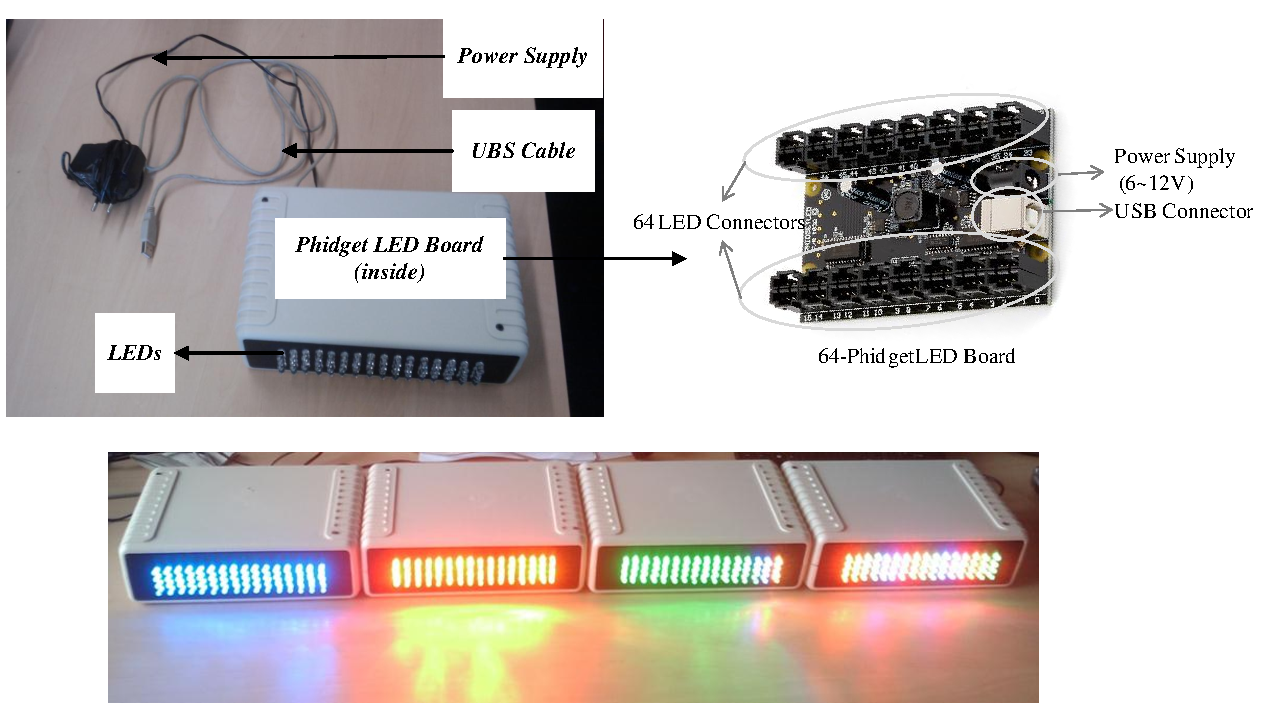
\includegraphics[width=250px]{lamp-KP}
\caption{Wall-wash lighting developed by TU/e SAN}
\label{wallwash}
\end{figure}

The decorative wall-wash lights consisted of four LED lamps, custom-built by the TU/e \ac{SAN} group, capable of generating coloured illumination on the wall of the room. The lamps are shown in Figure \ref{wallwash}, including a description of its components. A presence sensor determines the presence of a user in a designated area of the room and sends the presence information to the \ac{SIB}. The wall-wash lighting \ac{KP} is subscribed to this presence information, and its state is modified based on this information. There are two states updated on the \ac{SIB}: \texttt{Away} and \texttt{Present}. For example, when the \texttt{Present} state is specified, the Lamp \ac{KP} sends  the \texttt{ON} command to the wall-wash lighting, and the \texttt{OFF} command when the \texttt{Away} state is specified.  


\subsection{Connector object}
\label{Connector}
This device builds on the work done in the previous iteration by exploring another tangible approach for manipulating semantic connections. While devices are still identified with \ac{RFID} tags, the device itself is now mobile, and makes use of more meaningful interactions and feedback to establish and break connections.

\begin{figure}
\centering
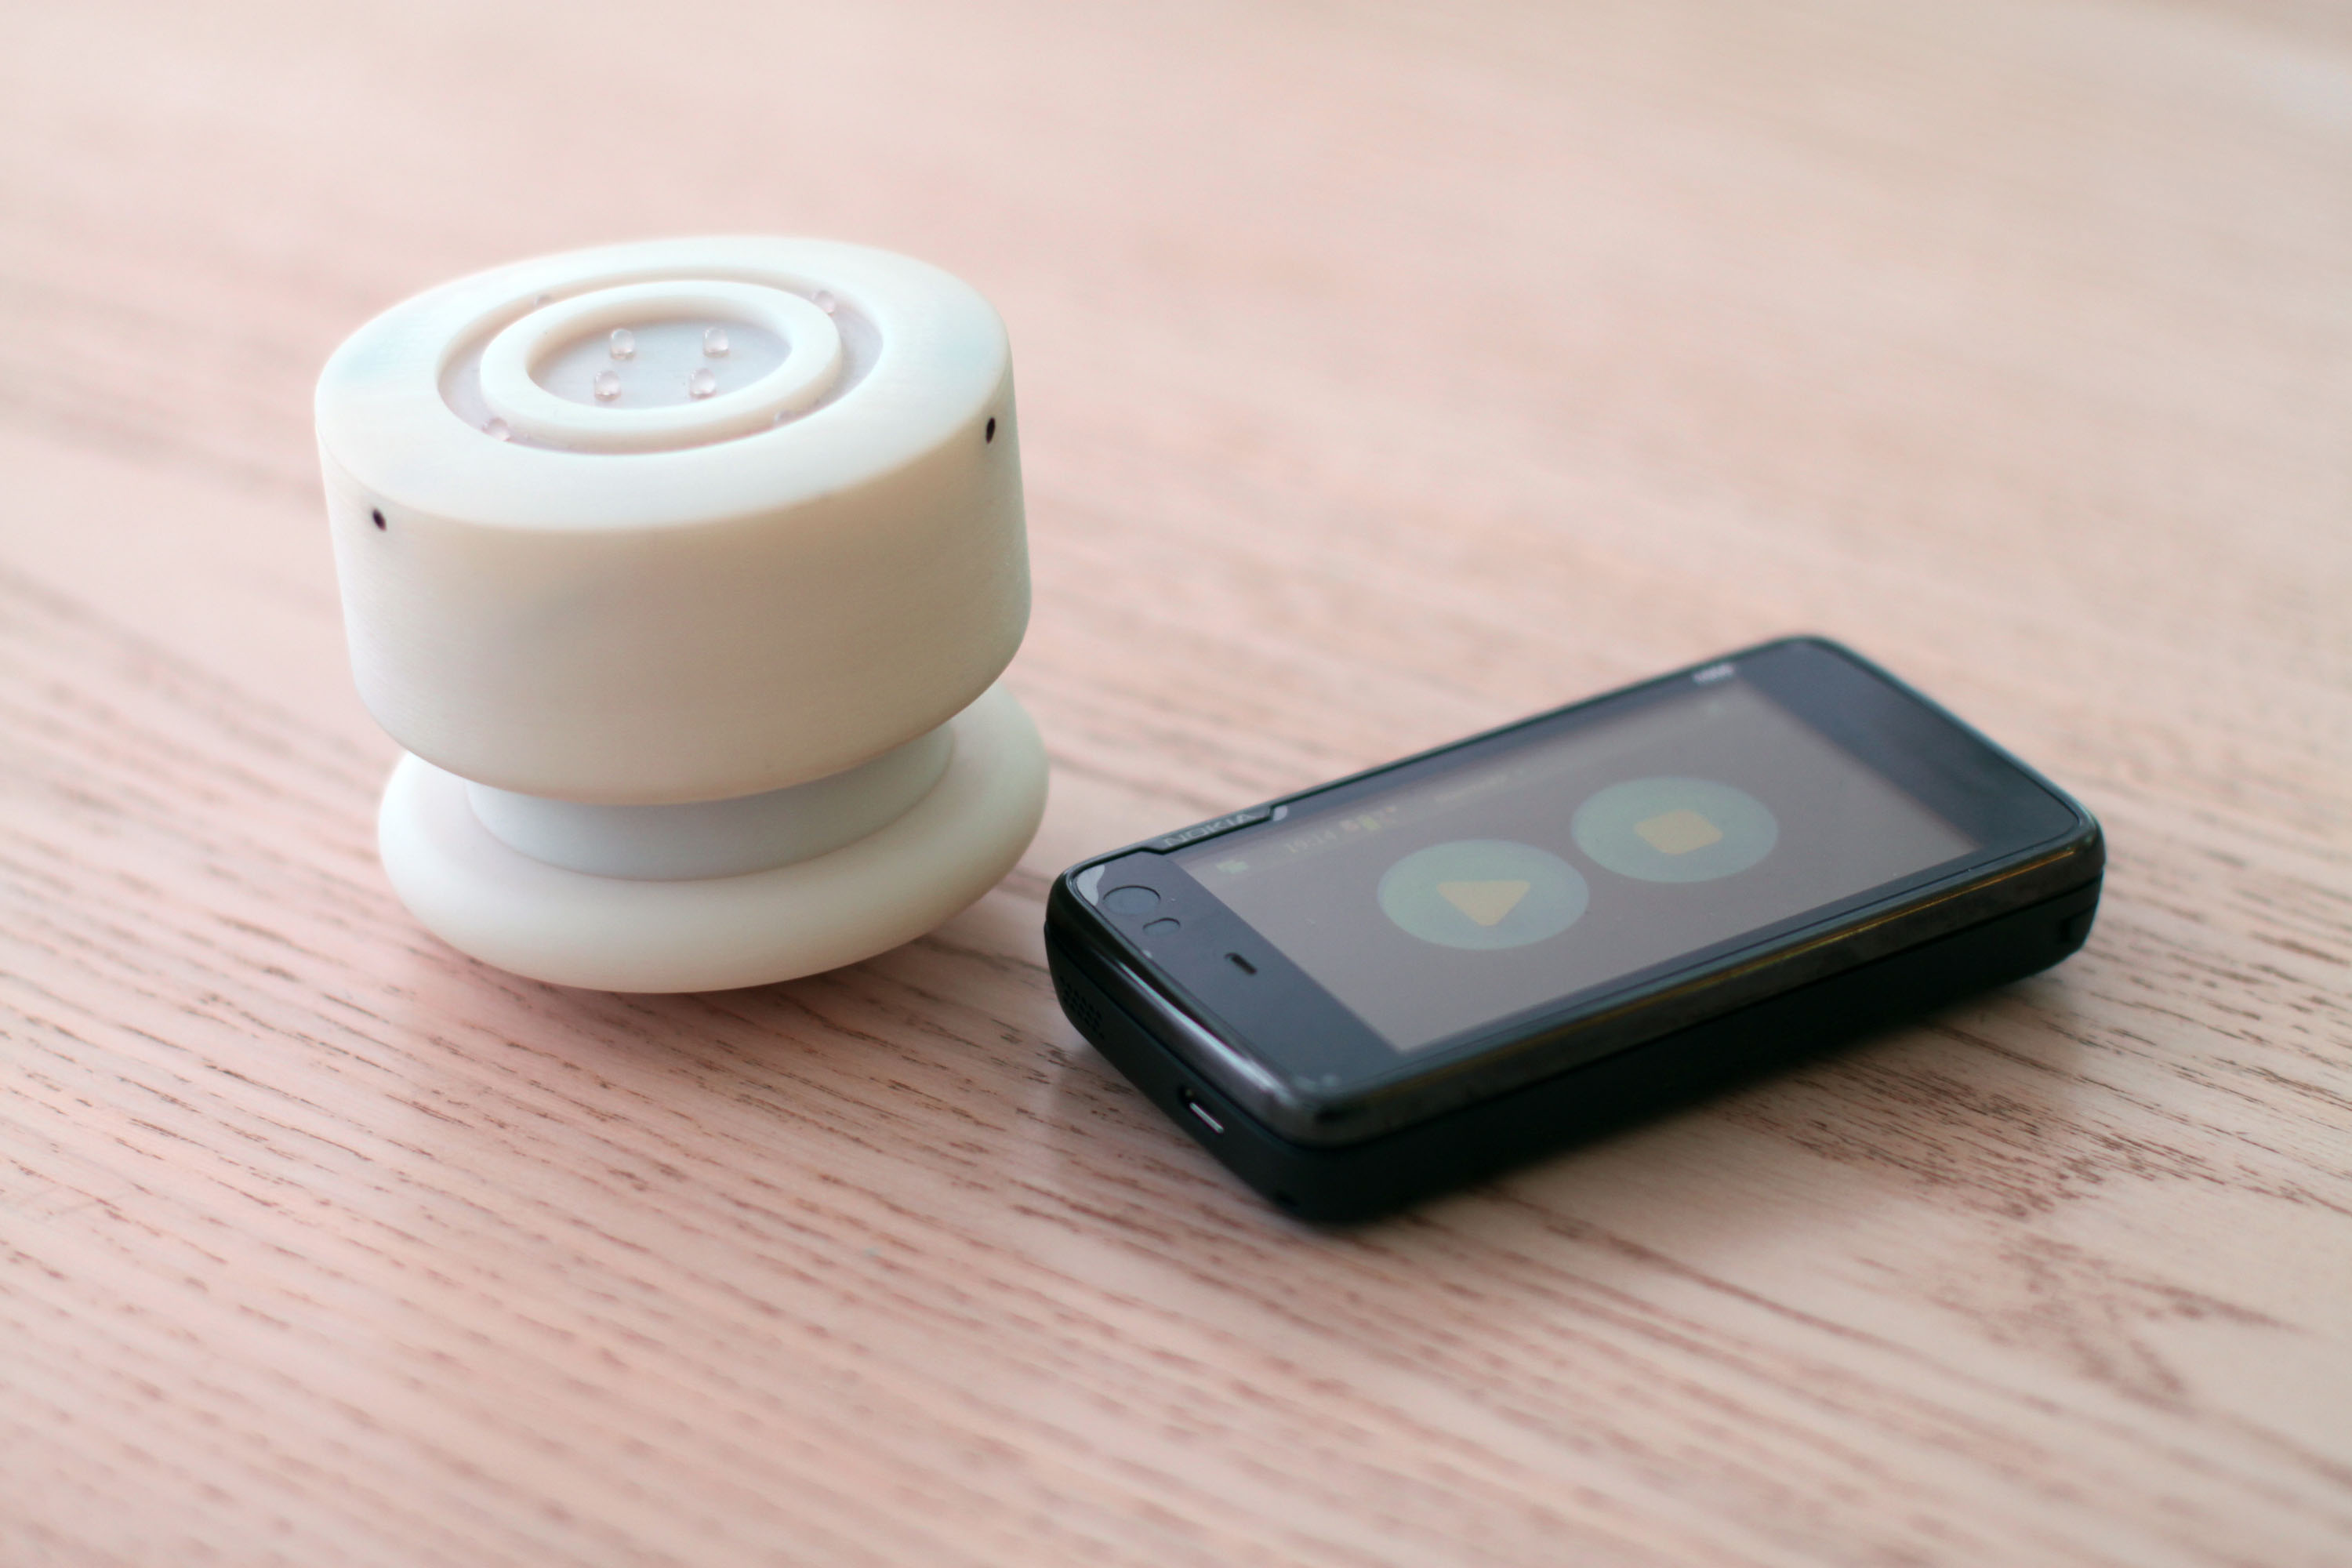
\includegraphics[width=300pt]{connector}
\caption{The Connector prototype and a smart phone used as a media player}
\label{connector}
\end{figure}

The Connector object, shown in Figure \ref{connector}, can be used to explore and manipulate semantic connections between different devices in the home environment. It is a handheld device that identifies devices, by scanning \ac{RFID} tags that are located on the devices themselves. By holding the Connector on top of the tag, users can explore the connection possibilities that are visualised with lights on top of the Connector. After holding the device in the \ac{RFID} field for a moment, the device-ID is locked and the other device to be connected can be selected in a similar fashion. With a push-to-click action a connection between two devices can be established. For removing an existing connection, the ring on the lower part of the device should be pulled until it clicks.

The cylindrical shape of the Connector is loosely inspired by that of a loupe or hand lens. By moving the connector over a tag, the connection possibilities can be ``read'' from the top of the cylinder. The display consists of two rings (made up of LEDs), each divided into 4 segments. The Connector supports several actions:

\begin{itemize}
	\item Explore - You can move it over an object or tag to see whether it is active.
	\item Select - A device or object can be selected by holding the connector close to or on a tag until the selection sequence is completed.
	\item Connect/disconnect - The connector can be compressed by pushing the top and the lower part together (connect), and it can be pulled, by pulling the lower part and the top part away from one another until it clicks (disconnect).
\end{itemize}   

When the tag is in the range of the Connector's \ac{RFID} field, it reads the tag and the first (yellow) light segment on top of the Connector will light up, serving as feedback that the Connector recognises the device. After holding the Connector over a device tag for a moment, a sequence starts, lighting up the second, third and fourth segment of the inner ring. After the device is recognised and selected, another device may be selected in a similar fashion. Now, the second ring of lights will start lighting up in sequence and one should wait until both rings are fully lit. Removing the Connector from the tag prematurely cancels the selection process.

When a connection between the selected devices is possible, both rings start flashing green. When no connection is possible, they will turn red. When a connection between the devices you scanned already exists, the rings will turn green. To make the connection, the Connector is compressed by pushing the top and lower part together, or by pushing the Connector down on the device it is touching, until it clicks. To remove an existing connection between two scanned devices, the ring on the lower part of the Connector should be pulled until it clicks. The rings will show a red light to indicate that the connection has been broken. The segments will turn off once the Connector is moved away from the device. Performing the opposite action of what is required to make or break a connection, cancels the procedure.

The Connector contains the following main components:

\begin{itemize}
\item Arduino Stamp 02
\item Innovations ID-12 125kHz RFID reader
\item SparkFun Bluetooth Mate Gold
\item 8 bi-colour LEDs
\item Switches
\item 3.3v LiPo battery (850 mAh)
\end{itemize}

Since only one tag is read at a time, we do not have the same issue identified in the previous iteration, and as such 125KHz tags could be used. The Connector prototype is made out of four separate pieces which are 3D printed. The lower part and the top part of the Connector can be moved inward and outward serving as a two-way spring-loaded switch. The prototype packages all the necessary components into one integrated device which is wirelessly connected to a computer using a Bluetooth connection. 


\subsection{Spotlight Navigation}\label{SpotlightNavigation}

\begin{figure}
\centering
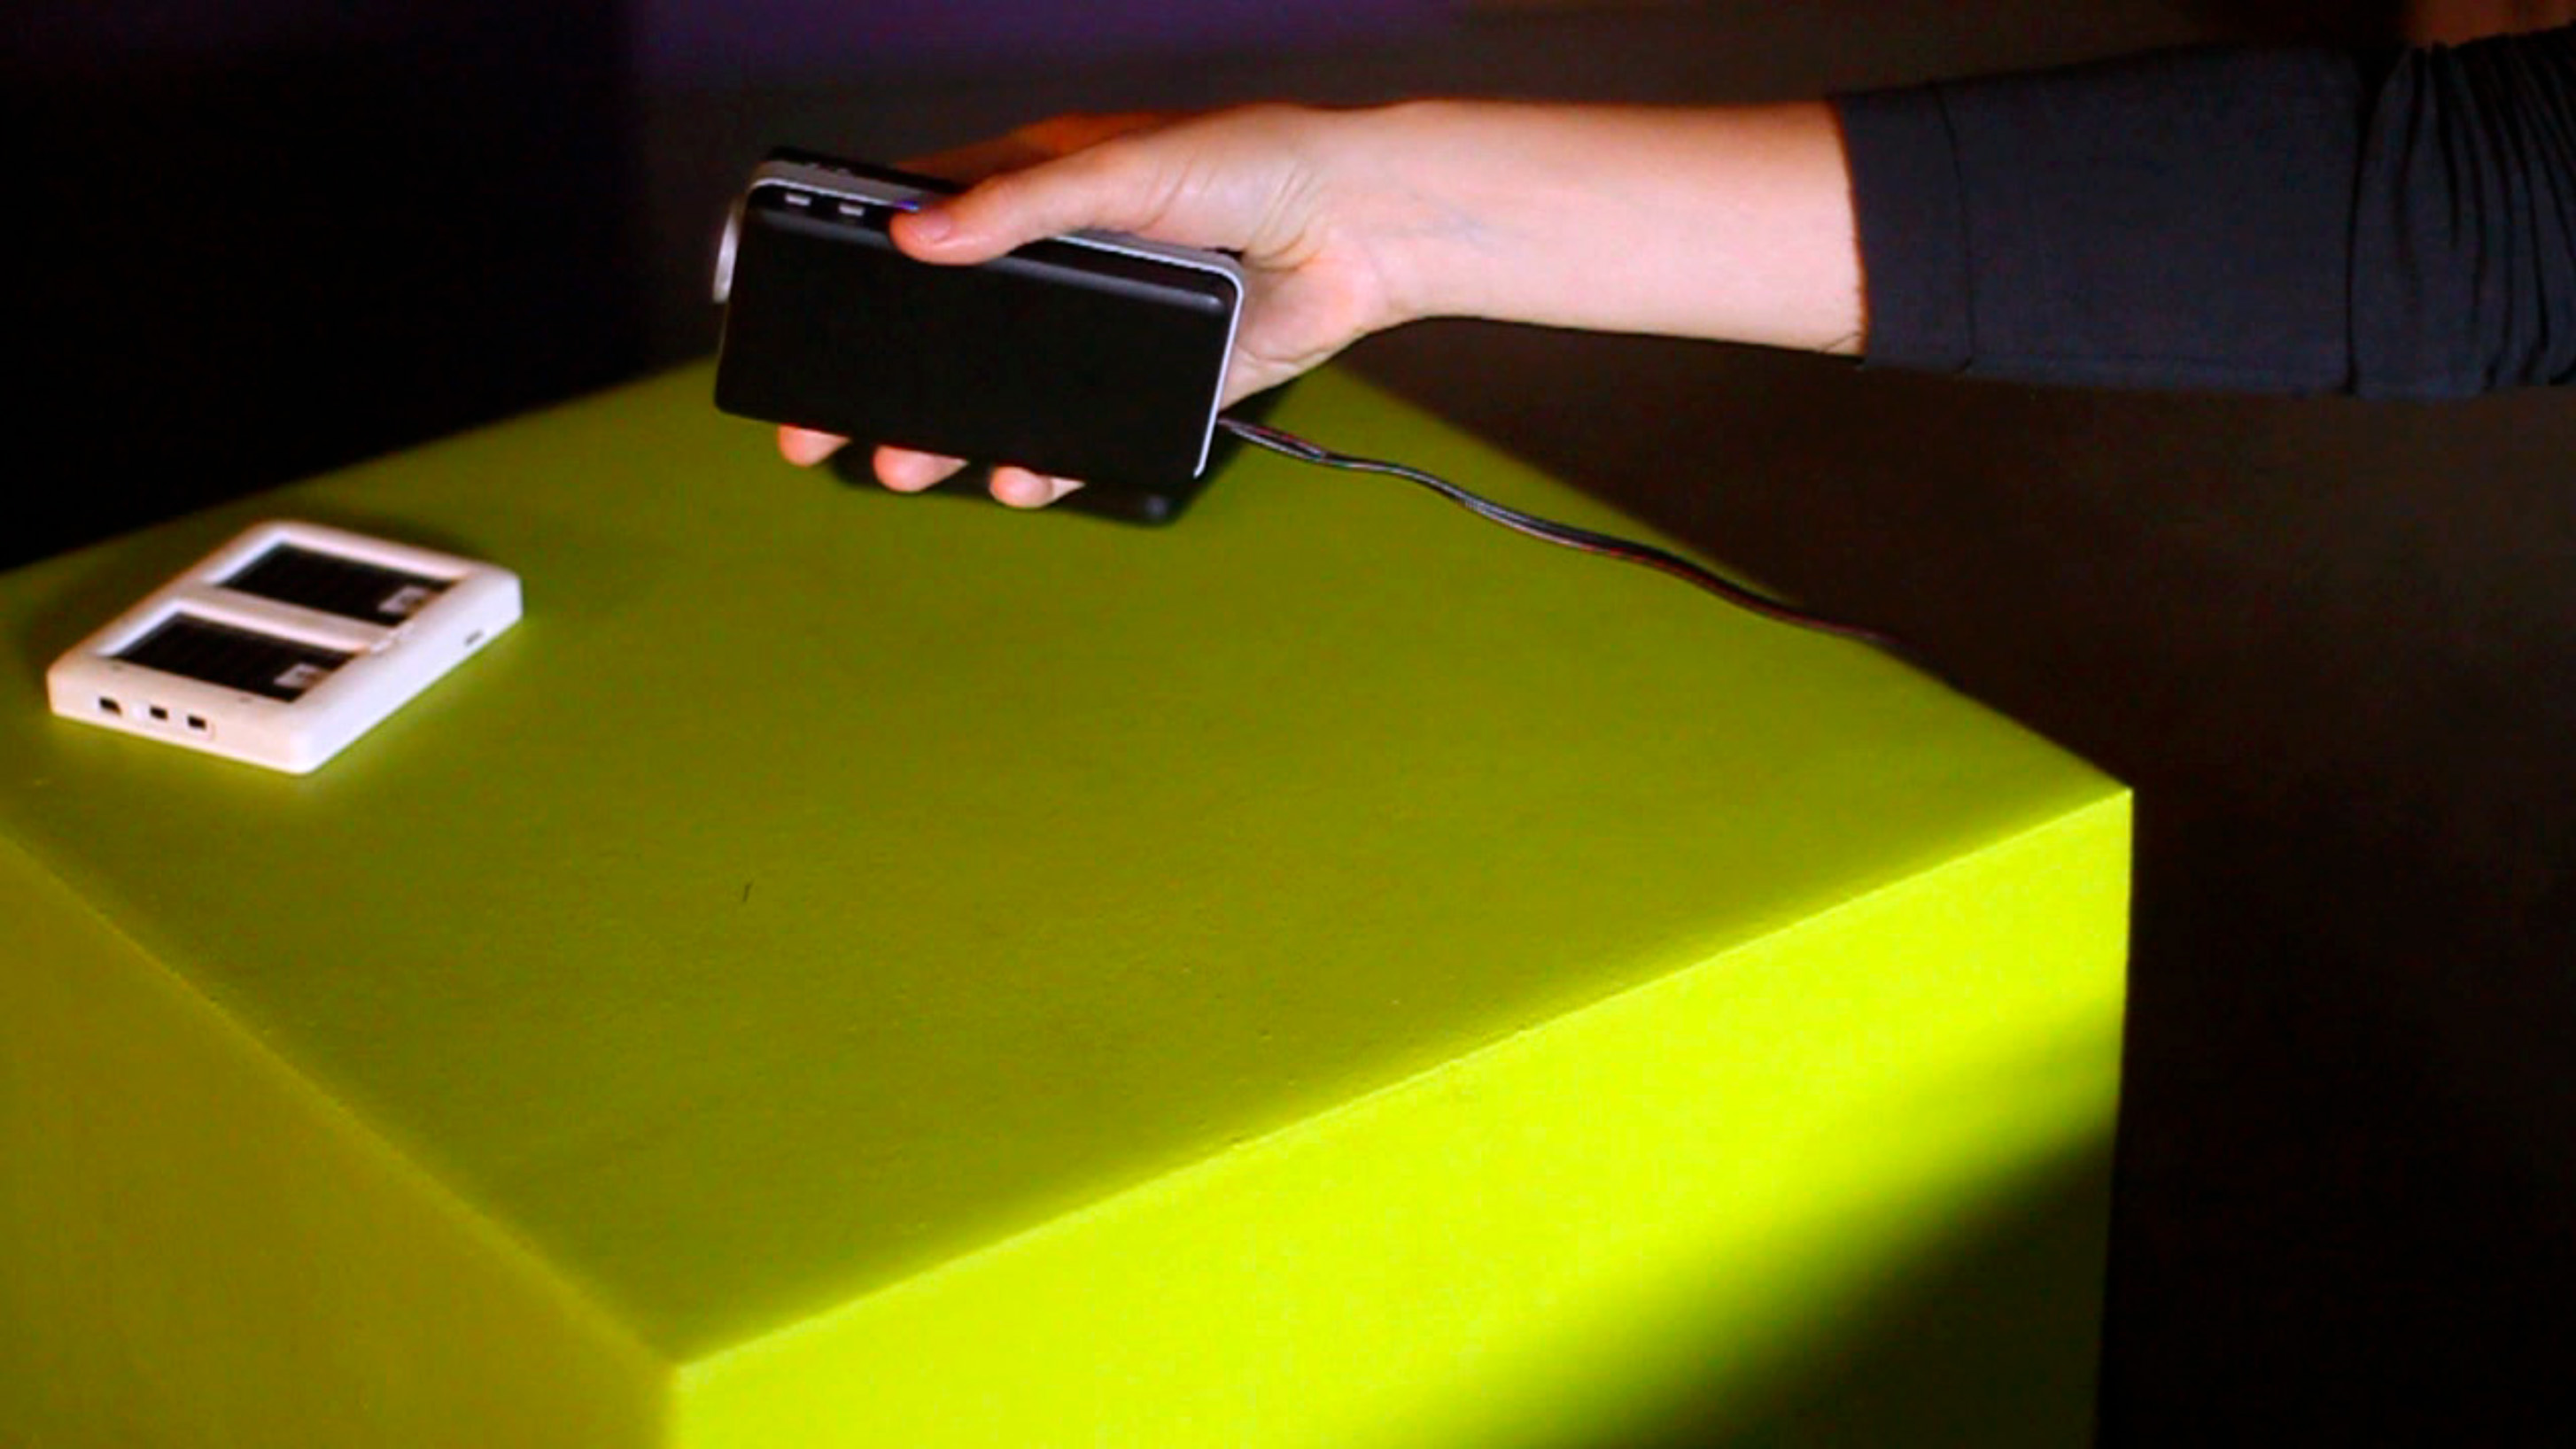
\includegraphics[width=300pt]{spotlightHand}
\caption{Spotlight Navigation prototype}
\label{projector}
\end{figure}

The Spotlight Navigation device, designed by Conante and shown in Figure \ref{projector}, is another approach to explore and manipulate connections between smart devices. With Spotlight Navigation, connection information contained in the smart space is projected into the real world, augmenting the real environment with virtual information, making it intuitively perceivable for users. Spotlight Navigation projects icons close to the actual devices in physical space. It allows for the creation of new connections simply by drawing lines between these icons, using a ``pick-and-drop'' action with a push-button on the prototype (press and hold the button when pointing at one device, move over the second device and release the button). Additionally the connection possibilities are projected between devices that allow for a connection, by changing the colour of the projected line (while the connection is being drawn) from yellow to green when the line's end is moved over the frame of the targeted device. When a connection is impossible, the connecting line will turn red and disappears as soon as the button is released.

Spotlight Navigation was invented as an intuitive way of accessing large data spaces through handheld digital projection devices \cite{Rapp2010,VanderVlist2012a}. Rather than directly projecting the equivalent of a small LCD display, Spotlight Navigation continuously projects a small portion of a much larger virtual pane or data space. It is the device's orientation that defines which part of the larger pane is selected for display. This is done in such a way that the virtual data appears to have a fixed location in the real world. By moving the projector's light spot over the wall, users make portions of the data space visible through intuitive, direct pointing gestures. This intuitiveness stems from the fact that the projected content always stays roughly at the same physical place, regardless of the orientation of the device. It becomes visible depending on whether it is in the projector's light cone or not. In other words, users have the impression that they are illuminating a part of a conceptually unbounded virtual data space, just as if they would be looking at hieroglyphs on a huge wall in a tomb with a flashlight. As people are familiar with operating flashlights, the operation needs no or little training. When accessing a data space with the device, users can zoom in and out of the data space by using a scroll wheel control, resulting in a pan-and-zoom user interface. To visualise the semantic connections in physical space, we rely on the symbolic meaning of colour, where green colour means ``proceed'' and red means the opposite. Using green, yellow and red lines we aim at referring to the ``existence'' of a connection, the ``possibility'' of a connection or to indicate that a connection is not possible. Figure \ref{projection} shows the projection when connecting two devices together.


\begin{figure}
\centering
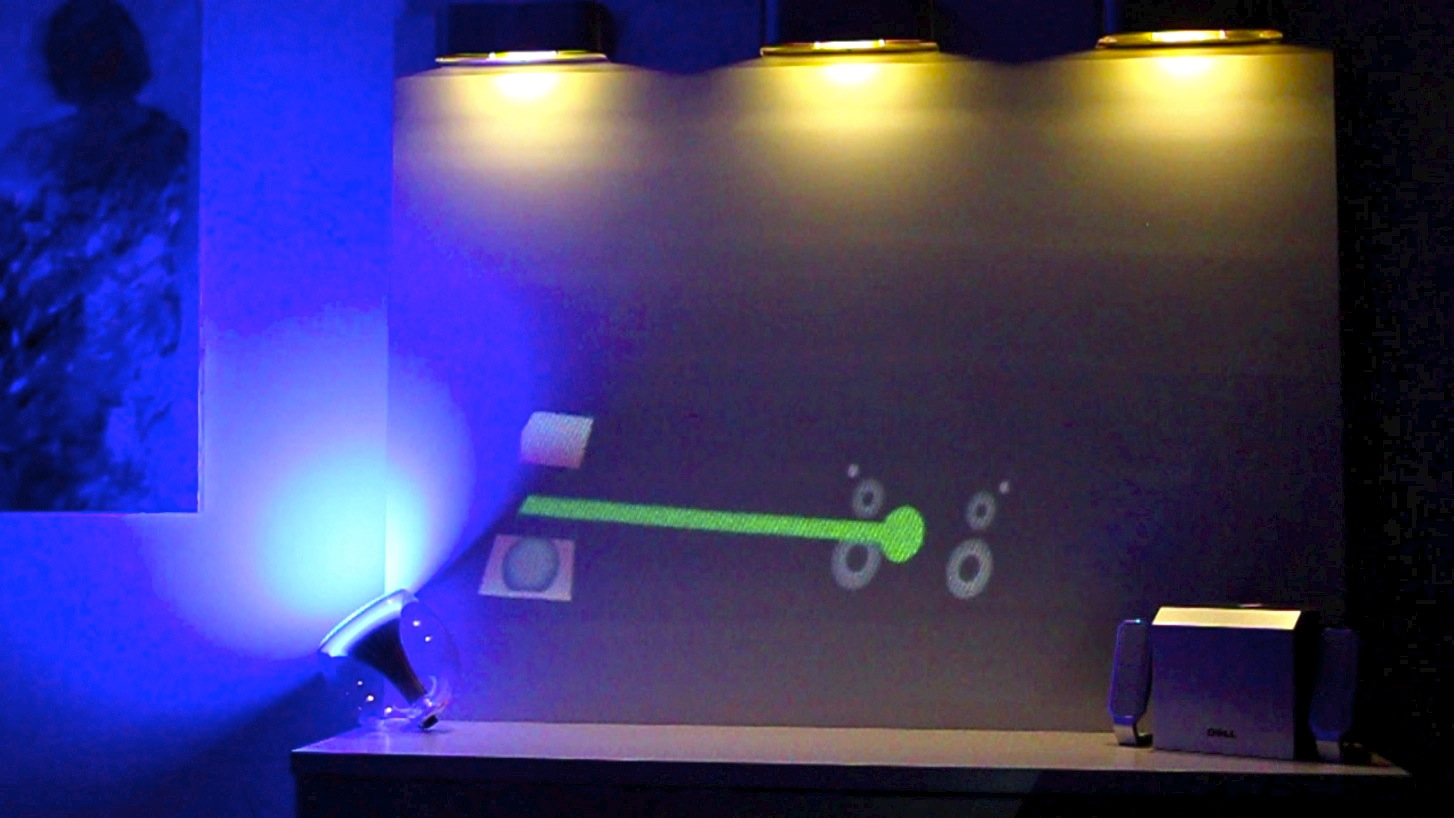
\includegraphics[width=300px]{projection}
\caption{Projection of the Spotlight Navigation when connecting two devices together}
\label{projection}
\end{figure}

With Spotlight Navigation, devices are identified by their physical location, relying strongly on \emph{natural mapping}. Connections are created simply by drawing lines between the devices. An erasing gesture with the Spotlight Navigation device pointed at an existing connection, breaks the connection. 

On a technical level, the operation is achieved through continuously measuring the orientation, and optionally also the position, of the device. Our prototype is using an inertial navigation module, also called an inertial measurement unit (IMU), that directly measure the orientation by means of accelerometers, gyroscopes and an electronic compass.

The Spotlight Navigation prototype is a fully embedded setup integrated into a 3D printed casing. The design of the casing was targeted at getting the smallest possible setup that could run on the integrated batteries. A dummy ring was added to the prototype to strengthen the semantics of a mobile projector. Figure \ref{projector} shows the prototype. Our current setup consists of the following components:

\begin{itemize}
\item OMAP3530 board (IGEP module)
\item Pico projector (Microvision SHOWWX)
\item Orientation sensor (Sparkfun 9DOF Razor IMU)
\item scroll wheel (with button press functionality)
\item two additional buttons
\item two 3.7v li-ion batteries (Nokia BL5J)
\end{itemize}

The OMAP3530 processor contains a 3D-graphics core (PowerVR) that is capable of
rendering the connection visualisations and device icons in real-time. The prototype required the object positions to be manually configured in space, as it did not contain a camera. By using a camera, as is planned for future versions, the intention is to recognise the identity and physical location of each device, so that it is no longer necessary to align the projected object icon with the location of its associated device.


\subsection{Lighting Device}

\begin{figure}
\centering
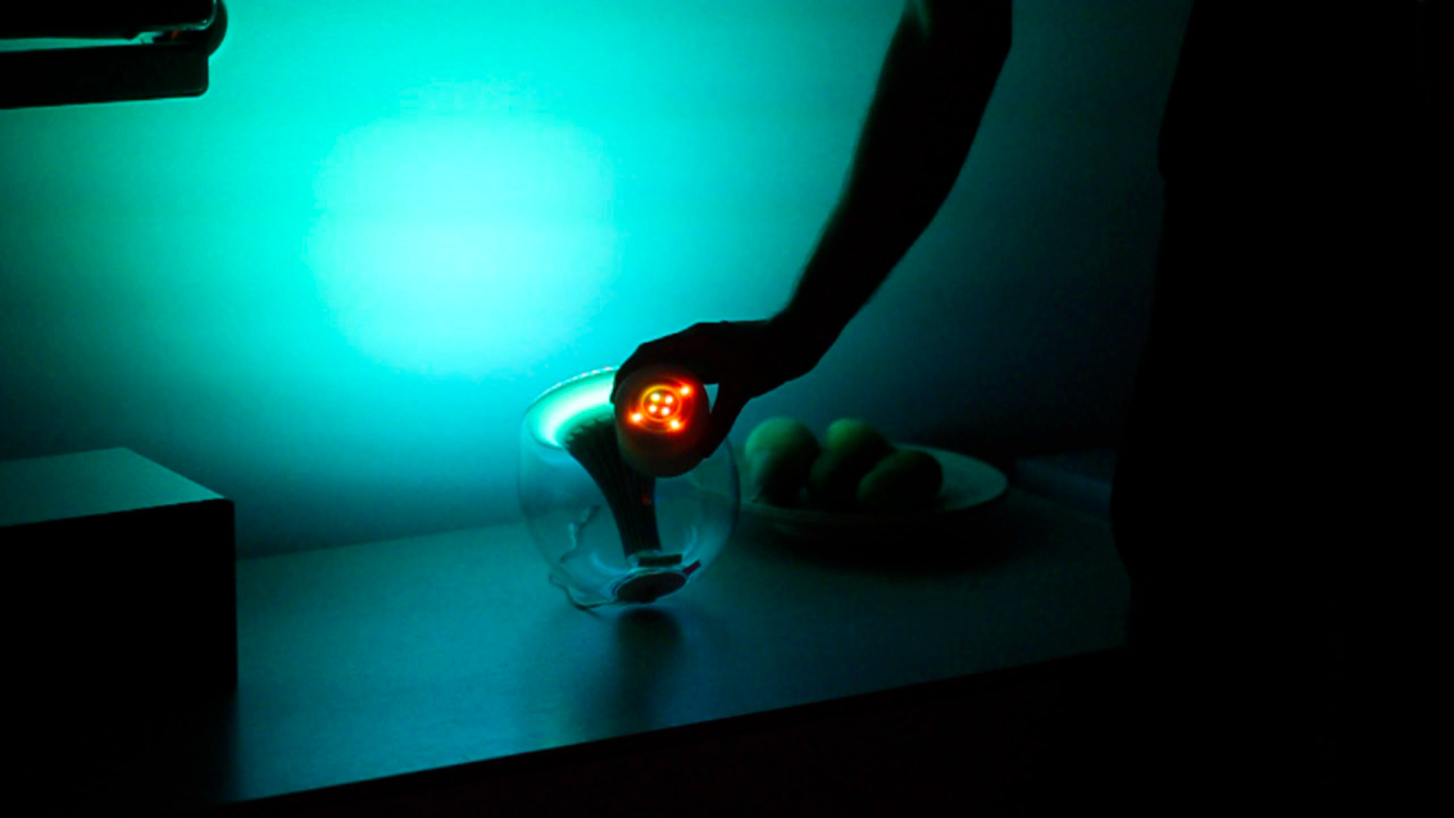
\includegraphics[width=300px]{LCscan}
\caption{Image showing the Connector scanning the lighting device.}
\label{LCscan}
\end{figure}

Philips created two lighting devices based on their LivingColors technology, that can be used to generate dynamic coloured lighting. Figure \ref{LCscan} shows the Connector object scanning a tag on the lighting device. These lighting devices accept a stream of RGB values and use the information to generate a sequence of coloured lighting. Using the media type descriptions introduced above, we can describe a lighting device as follows: 

\begin{minted}{turtle}
LightingDevice rdf:type SmartObject .
LightingDevice acceptsMediaType RGBValues .
LightingDevice rendersMediaAs Lighting .
\end{minted}

In the scenario there exists a permanent semantic connection between the two lighting devices. This means that when dynamic lighting is generated on one device, the same lighting will be displayed on the other device.

%The Bonding Device accepts dynamic lighting information in the form of a stream of RGB values. What makes this scenario interesting is that the mobile device itself is not capable of transmitting these RGB values, but the Sound/Light KP (a virtual device in the smart space) is. The Sound/Light KP acts as a semantic transformer, converting the music stream generated by the mobile device into the RGB values required by the Bonding Device. From the user's point of view, the only \textit{required} connection is that between the mobile device and the Bonding Device, while the smart space takes care of the rest.



\section{Implementation}
\label{D2Implementation}

The goals of the Smart Home pilot were as follows:

\begin{itemize}
	\item Conduct a pilot study with users in a setting that resembles a real home
	\item Demonstrate the system to stakeholders and other interested parties
	\item Serve as a feasibility study
	\item Test how stable the implementation would be when it would be running for a full week
	\item Serve as a experimental setup for user experiments
\end{itemize}

%In this section we describe implementation details of how the concepts of the theory are modelled

\begin{figure}
\centerline{
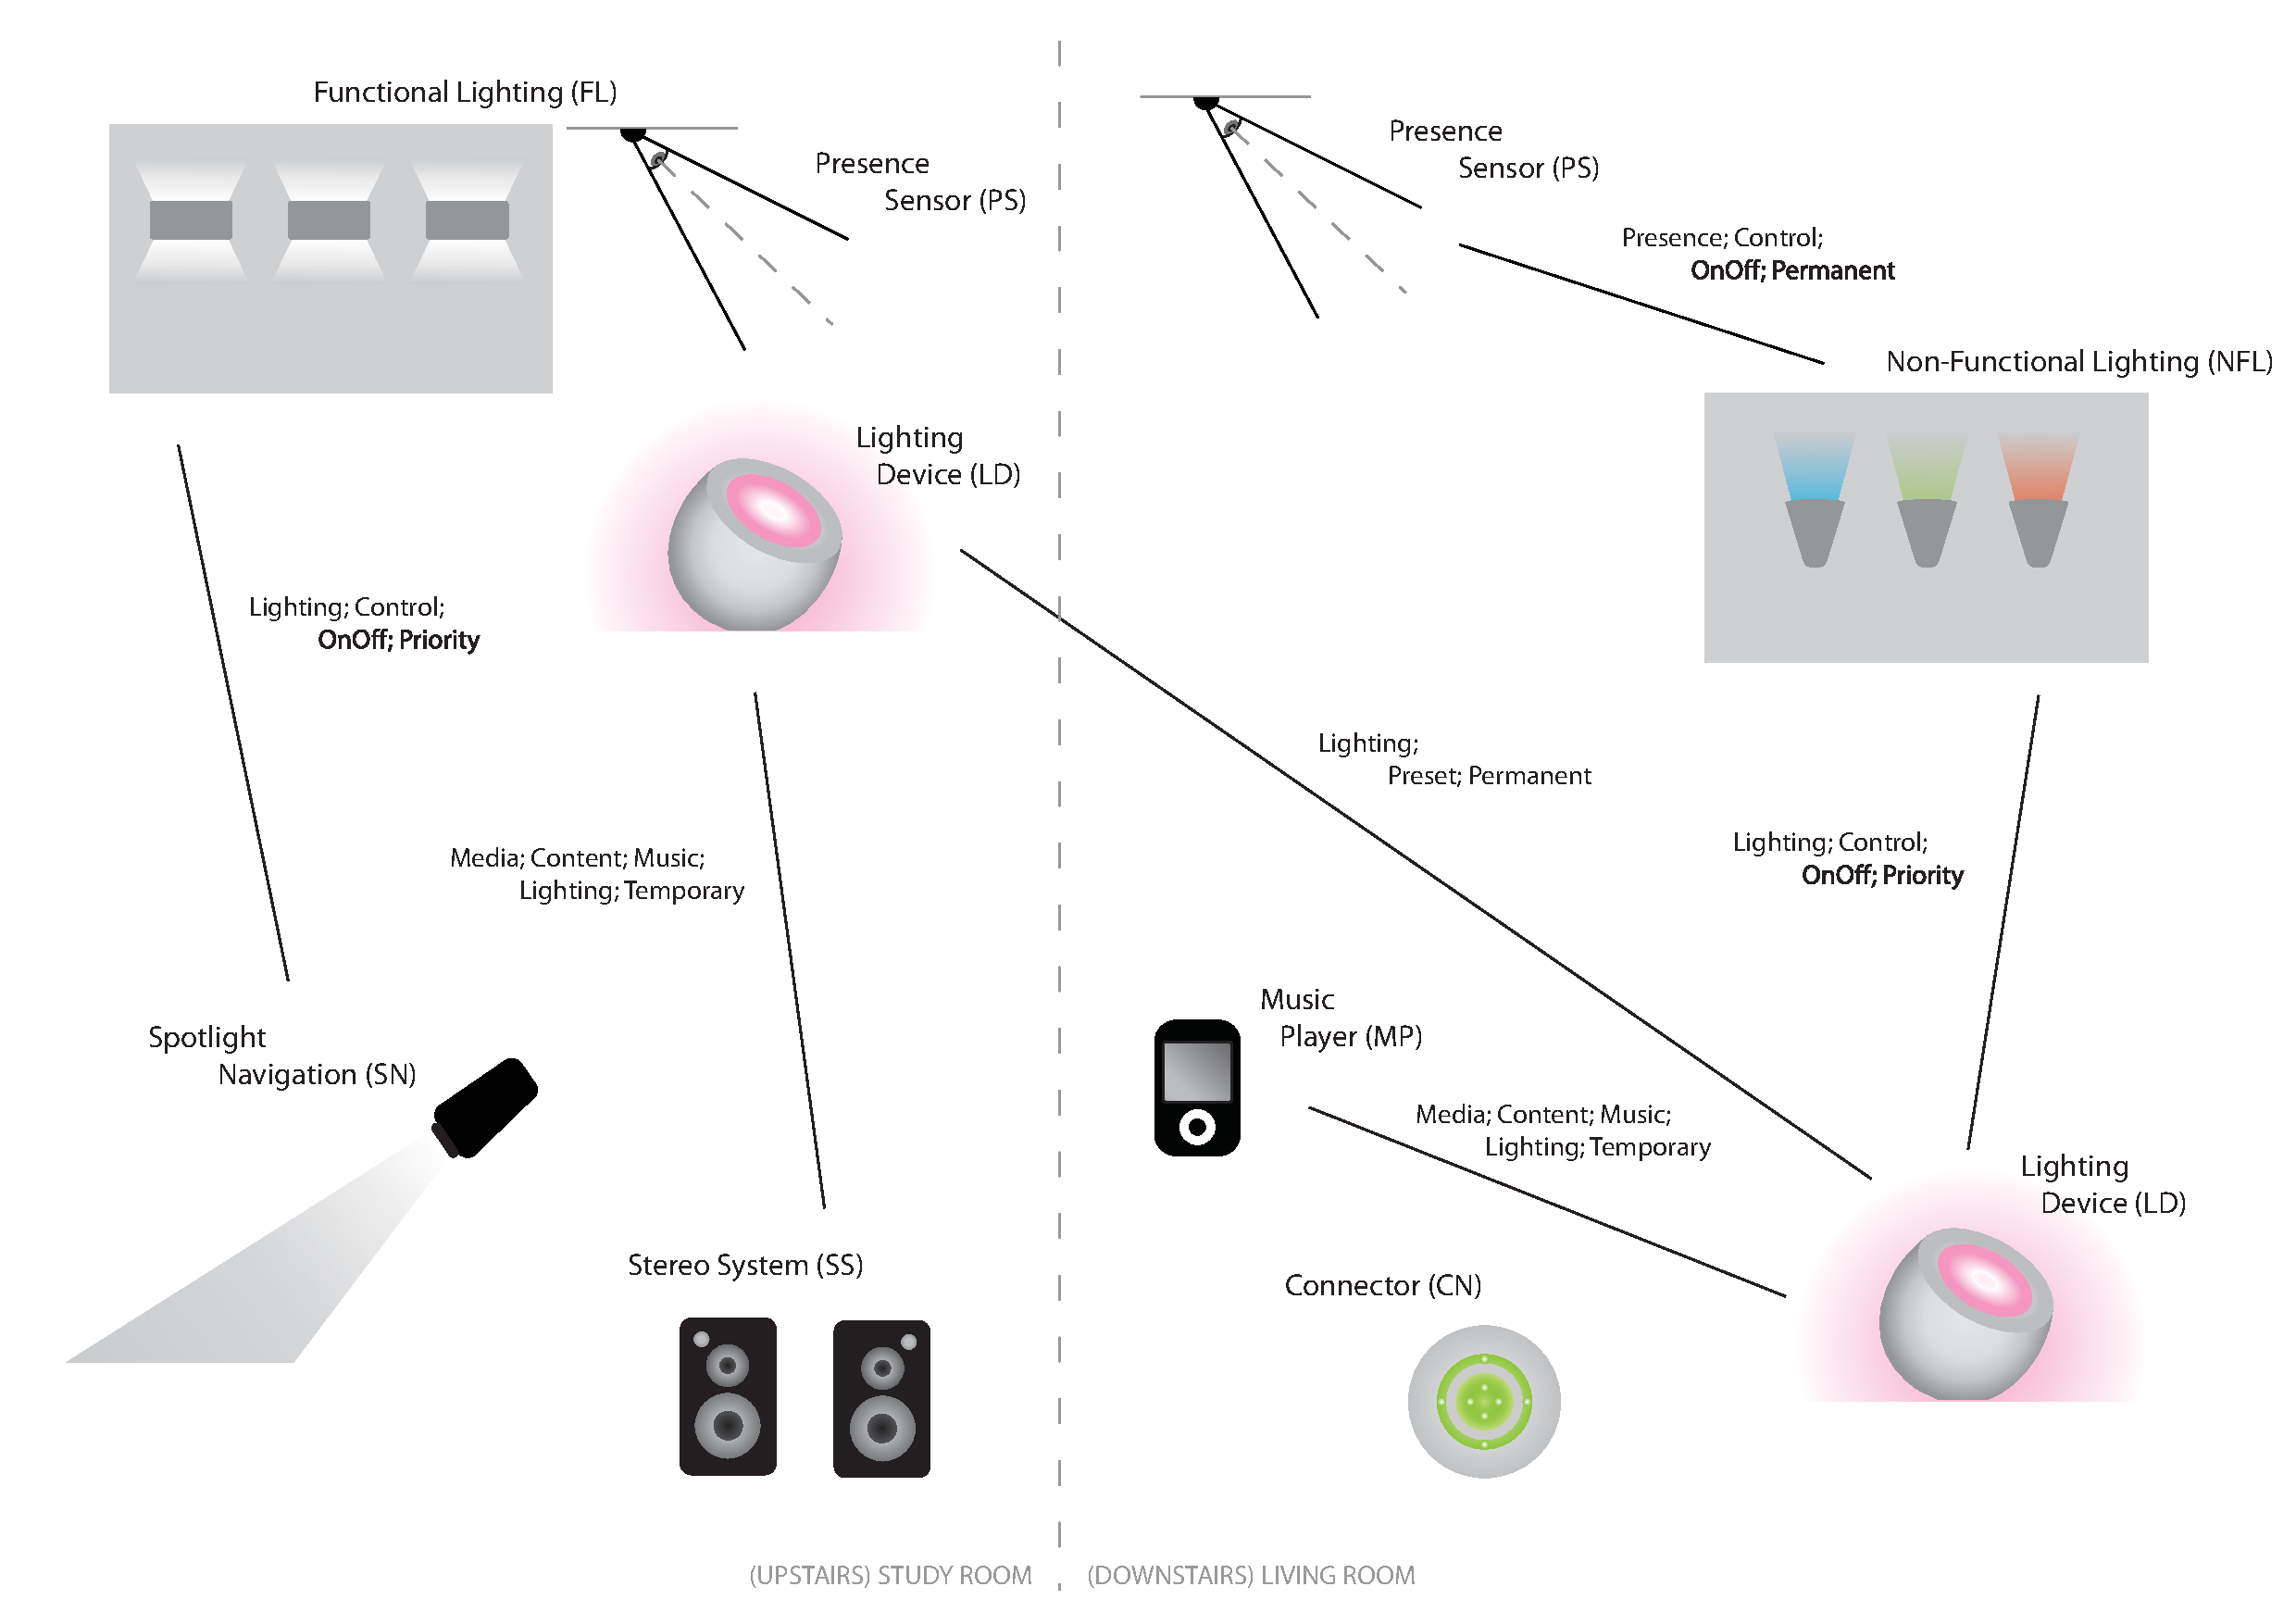
\includegraphics[width=\paperwidth-40mm]{pilotSetup}}
\caption{The devices and their connections as used in the system}
\label{pilotSetup}
\end{figure}

Figure \ref{pilotSetup} shows a brief overview of the different parts of the system. The experiment took place in two rooms, the study and the living room of the Experience Lab on the High Tech Campus in Eindhoven. During the pilot, users interacted with various automated and interactive appliances and devices defined as smart objects. There exist several semantic connections between the smart objects, for example the media-content connection between the phone and the lighting device, and the lighting-control connection between the lighting device and the non-functional lighting. Some of these connections can be explicitly interacted with through two interaction devices: a Spotlight Navigation device placed in the study of the pilot setup upstairs, or a Connector device placed in the living room of the pilot setup downstairs. 

% The Spotlight Navigation device is a mobile device containing a pico projector that visualises connection possibilities between devices in the environment. By using direct pointing gestures with the device in the user's hand, users can intuitively explore and manipulate the virtual network connections as if they are part of the user's real world environment. The Connector device follows a tangible interaction approach, enabling users to physically select devices in their environment and directly view and manipulate the connections in a simple, universal way. It is a hand-held device that identifies devices by scanning RFID tags that are located on the devices themselves. By holding the Connector on top of the tag, users can explore the connection possibilities that are visualised with lights on top of the Connector. After holding the device in the RFID field for a moment, the device-ID is locked and the other device to be connected can be selected in a similar fashion. With a push-to-click action a connection between two devices can be established. For removing an existing connection, the ring on the lower part of the device should be pulled until it clicks. 

 %A video of the Smart Home pilot is available online\footnote{}. (Not public)



In the Smart Home pilot, media content is shared among several smart objects in a smart home setting. Music can be shared between a mobile device, a stereo speaker set and a lighting device that can render the mood of the music with coloured lighting. The music experience is also shared remotely between friends living in separate homes through the lighting device. This light and music information is shared between the two lighting devices. Other lighting sources, like the smart functional lighting (FL, Figure \ref{pilotSetup}) and the smart wall wash lights (NFL, Figure \ref{pilotSetup}) are sensitive to user presence and the use of other lighting sources in the environment. The setup was built using the \ac{SOFIA} software platform as is described in Chapter \ref{SoftwareArchitecture}. A diagram showing the technical details of the Smart Home pilot is shown in Figure \ref{SmartHomePilotDiagram}. It gives an indication of the variety and complexity of the hardware platforms, operating systems and wireless protocols that were used.

%alternative is to use pdfpages, but textpos seem to work fine
% \newpage
% \thispagestyle{empty}
% \begin{textblock*}{\paperwidth-10mm}(10mm,10mm)
%         \begin{figure}
% 		\centering
% 		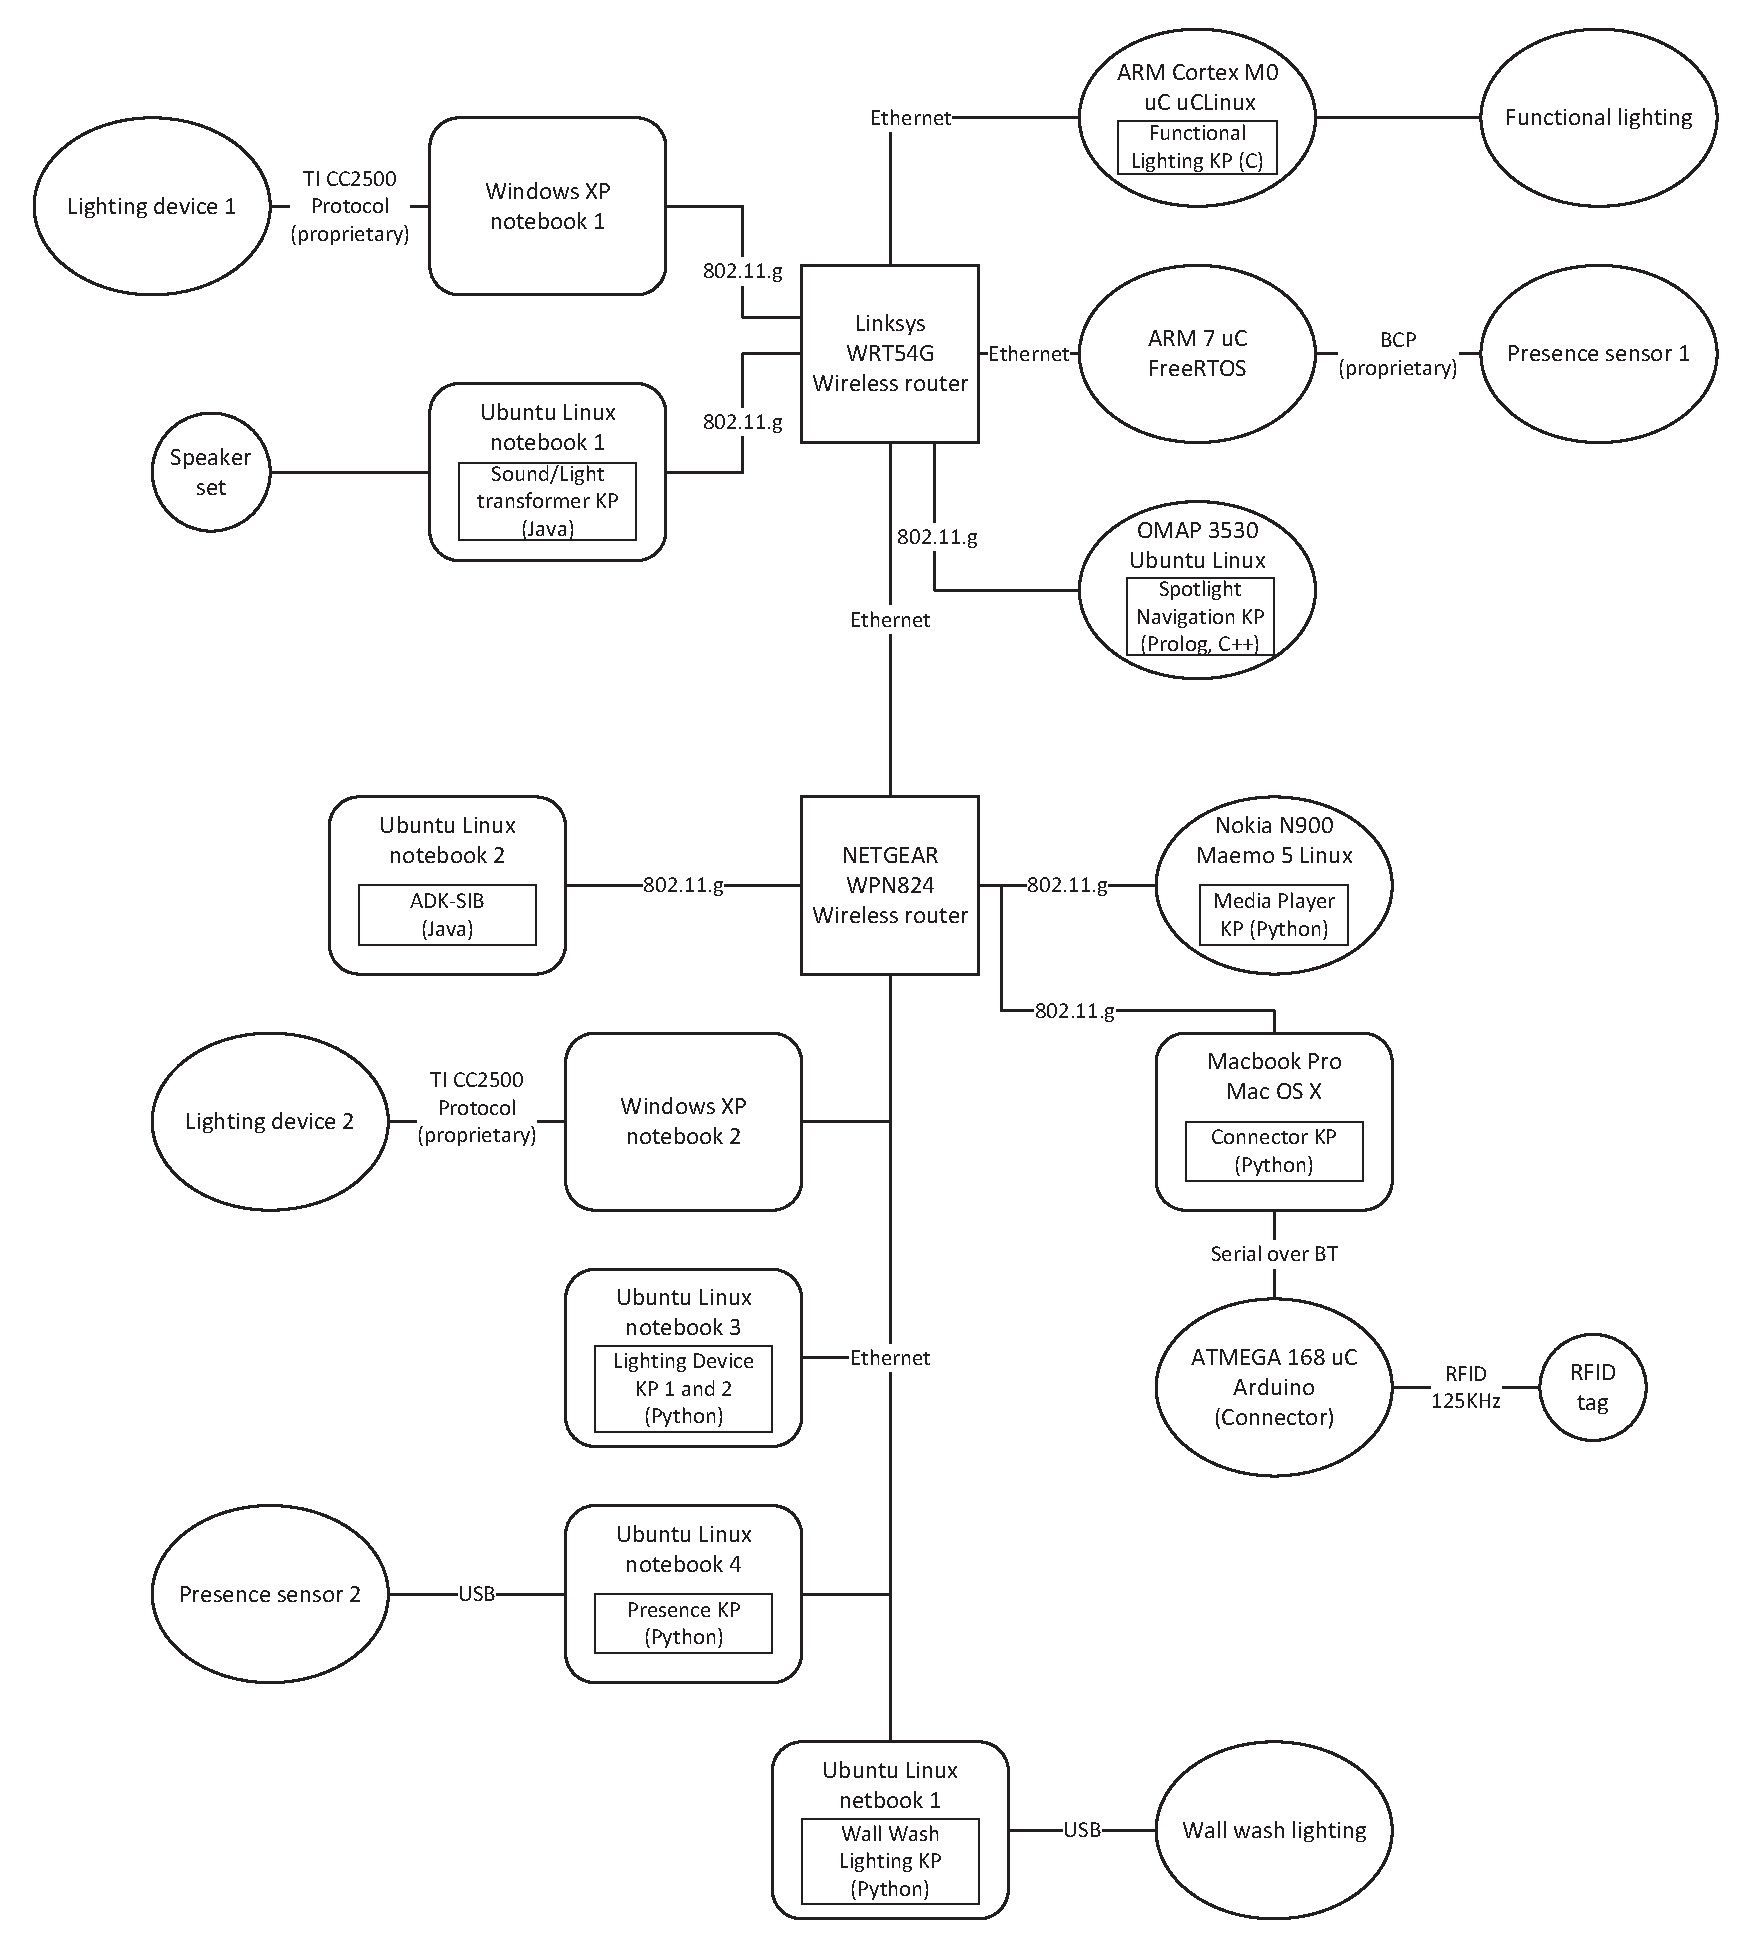
\includegraphics[width=\paperwidth-20mm]{SmartHomePilotDiagram}
% 		\caption{Technical details of the Smart Home pilot}
% 		\label{SmartHomePilotDiagram}
% 		\end{figure}
% \end{textblock*}
% \mbox{}\newpage


\begin{figure}
		\centerline{
		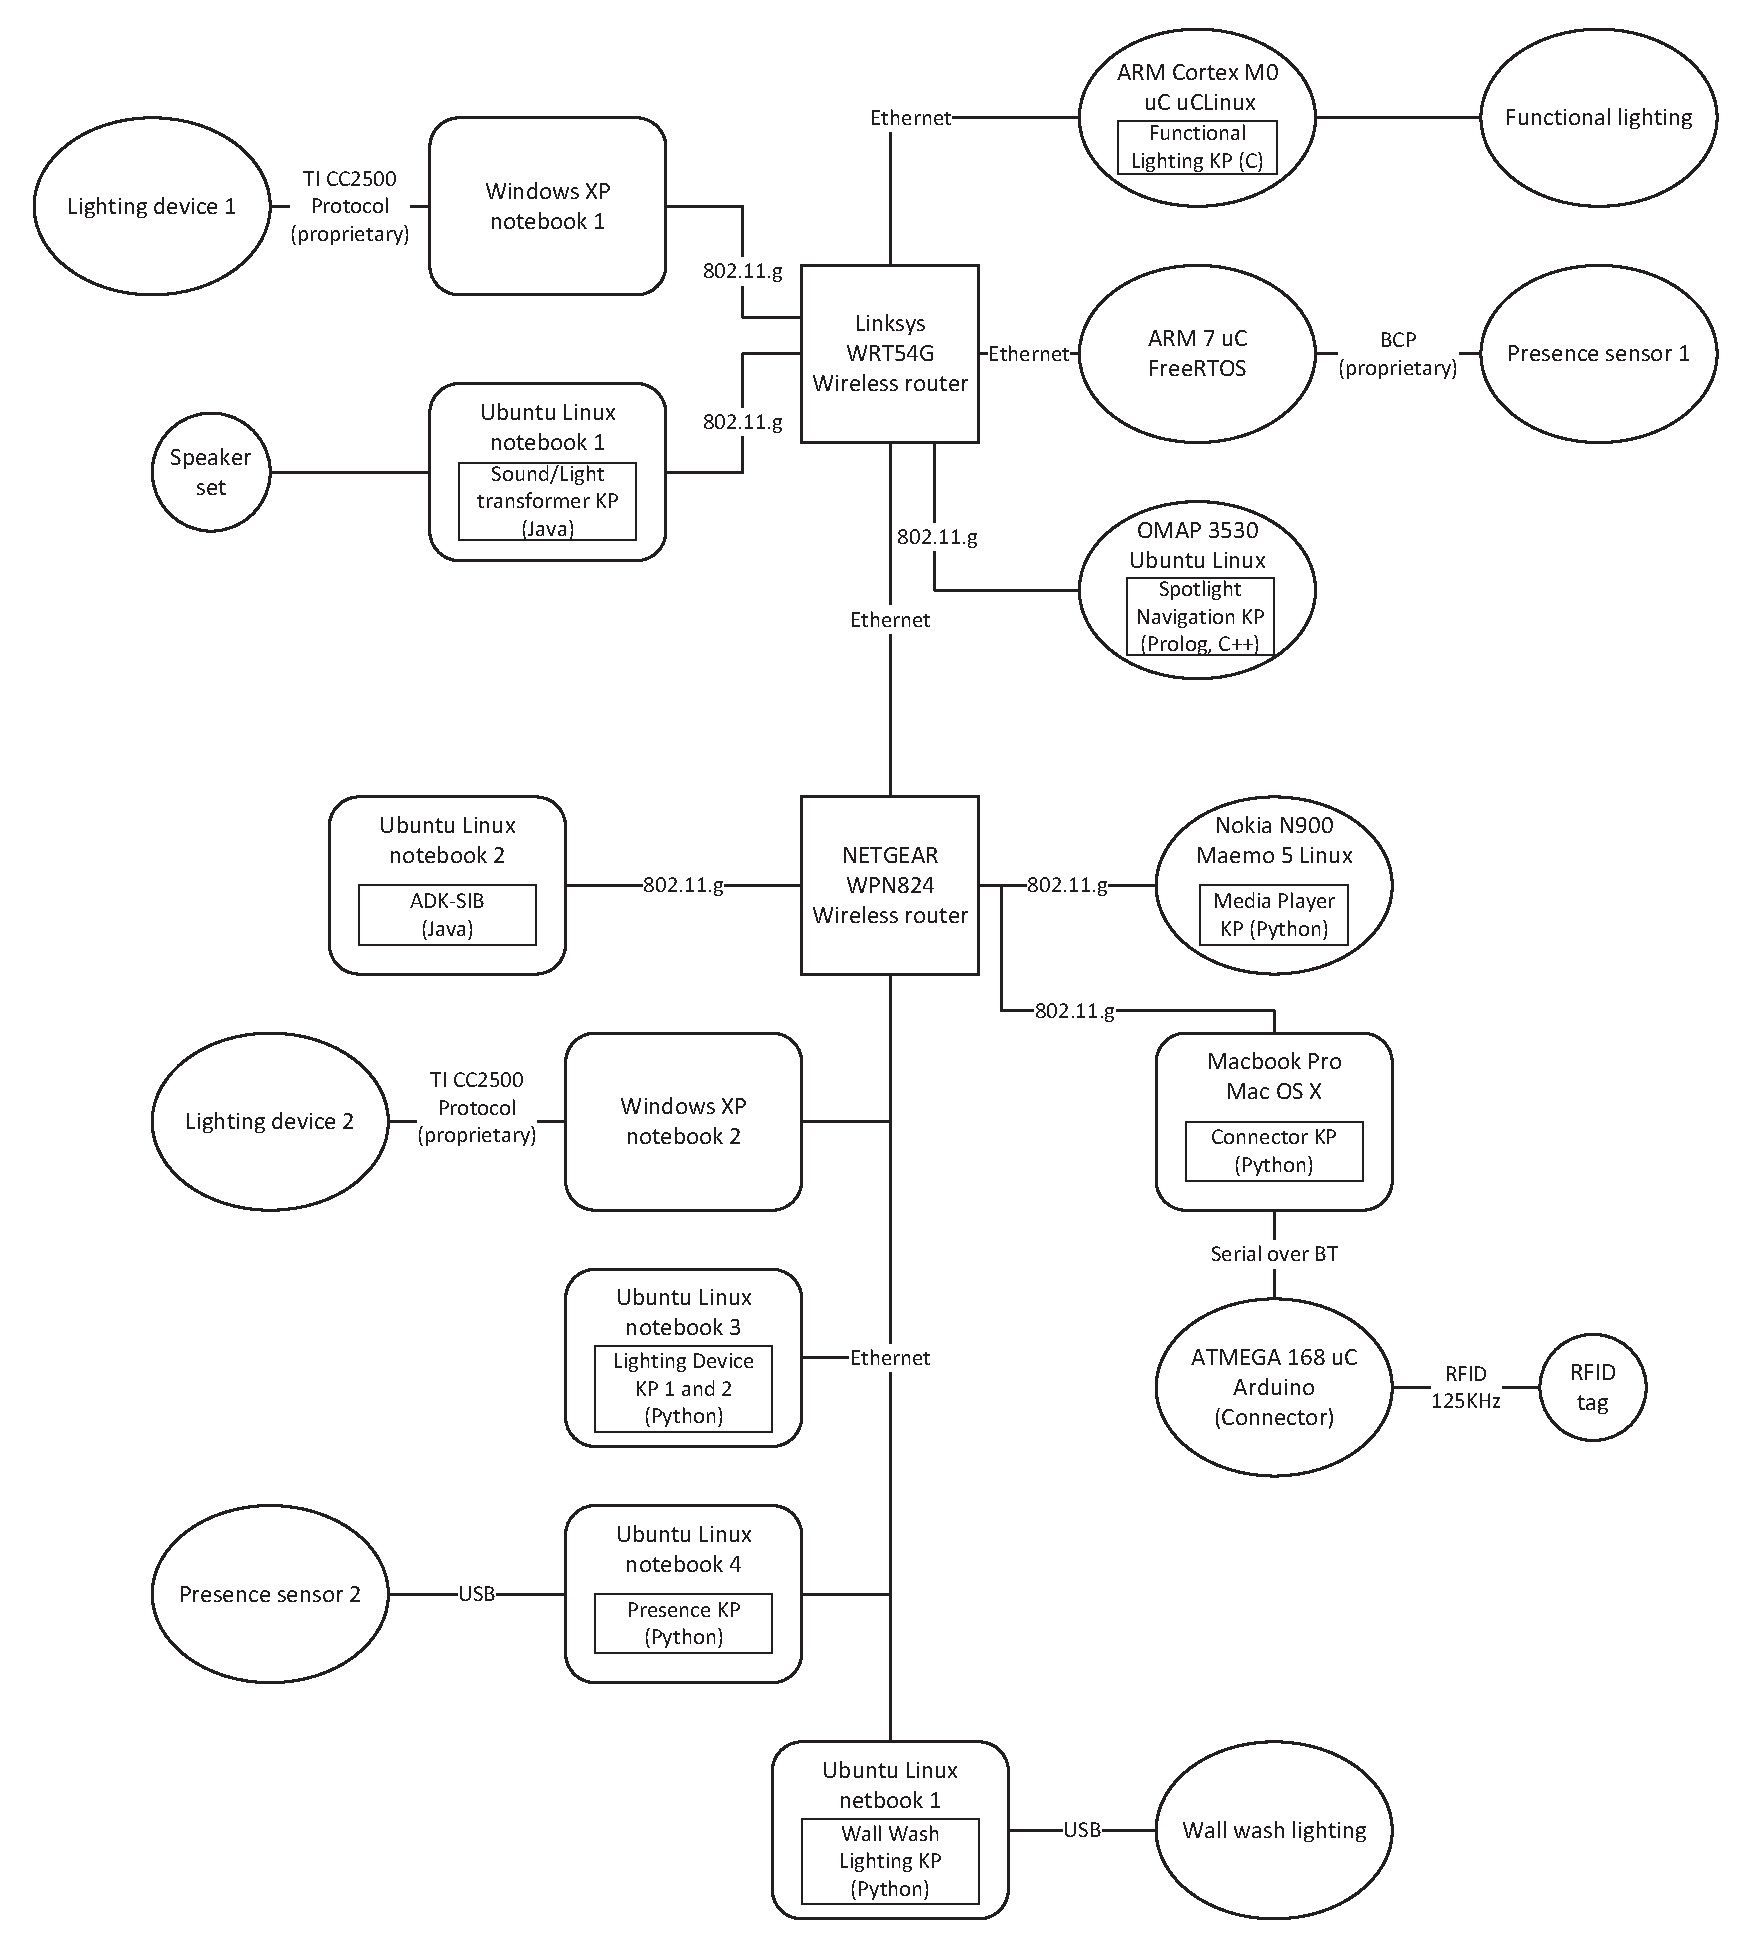
\includegraphics[width=\paperwidth-40mm]{SmartHomePilotDiagram}}
		\caption{Technical details of the Smart Home pilot}
		\label{SmartHomePilotDiagram}
\end{figure}



% from deliverable
% During the pilot, users experience a smart space with various automated and interactive appliances and devices (smart objects). The appliances in the smart space are interoperable, sensitive to changes in their environment and exchange information with one another. There are several explicit and implicit relations between the smart objects, of which some can be explicitly viewed or manipulated with the Spotlight Navigation device or the Connector device, available in two different locations.
% In the Smart Home Pilot, media content is shared among several devices in a smart home setting. Music can be shared between a mobile device, a stereo speaker set (connected to the smart space through a Sound/Light KP) and a Family Bonding Device that as one of its capabilities can render the mood of the music with coloured lighting. The music experience is also shared remotely between friends living in separate homes through the Bonding Device. This light and music information is shared between the two lighting devices. Other lighting sources, like the smart functional lighting from NXP and the smart wall wash lights (TU/e-SAN) are sensitive to user presence and the use of other lighting sources in the environment.

% We illustrate our implementation of semantic transformers by means of a use case scenario, where the semantic transformers were introduced as part of a smart home pilot (as defined in the SOFIA project). 

%In the Smart Home pilot, media content is shared among several devices in a smart home setting. Music can be shared between a mobile device, a stereo speaker set  and a lighting device that can render the mood of the music with coloured lighting.

\subsection{ADK-SIB}
\label{adk-sib}
In this iteration a new \ac{SIB} developed within the \ac{SOFIA} project was used, called the ADK-SIB. The ADK-SIB is a Jena-based\marginpar{The Jena framework was first mentioned in Section \ref{Jena}.} \ac{SIB} written in Java and runs on the \ac{OSGi} framework. Some modifications were made to the standard ADK-SIB provided by the \ac{SOFIA} project, such as reasoning support added with the TopBraid SPIN API 1.2.0\footnote{http://topbraid.org/spin/api/}. To run the \ac{SIB} from the \ac{OSGi} prompt, the \ac{SIB} and TCP/IP gateway is started separately as services:

\begin{minted}{console}
sspace create -sib -name=test
sspace create -gw -name=testgw -type=TCP/IP -idSib=1
sspace start -sib -id=1
sspace start -gw -id=1
\end{minted}

The \ac{SIB} and gateway are linked with one another through their IDs, enabling multiple \acp{SIB} and gateways to run on the same machine. \ac{OSGi} services have to be deployed as plugins from within the Eclipse development framework.

Reasoning on information contained within the \ac{SIB} was performed using \ac{SPIN}\footnote{http://www.spinrdf.org}. With SPIN, rules are expressed in \ac{SPARQL}, the W3C recommended \ac{RDF} query language, which allows for the creation of new individuals using CONSTRUCT queries. \ac{OWL} inferences for the \ac{OWL} 2 \ac{RL} profile were executed by using \ac{SPIN} rules\footnote{ http://topbraid.org/spin/owlrl-all}. OWL 2 RL is a syntactic subset of OWL 2 that is amenable to implementation using rule-based technologies. According to the OWL 2 RL W3C page\footnote{http://www.w3.org/TR/owl2-profiles/\#OWL\_2\_RL} the OWL 2 RL profile is aimed at applications that require scalable reasoning without sacrificing too much expressive power. 

\subsection{Semantic matching of media types}
\label{SemanticMatching}

A semantic transformer, called the Sound/Light KP, accepts a music stream as input and generates a stream of RGB values based on an analysis of the music stream. The Sound/Light KP is described as follows:

\begin{minted}{turtle}
SoundLightKP rdf:type SemanticTransformer .
SoundLightKP acceptsMediaType Audio .
SoundLightKP transmitsMediaType RGBValues .
SoundLightKP  hasIdentification id4321 .
id4321 ofIDType IPAddress .
id4321 idValue "192.168.1.4:1234" .
\end{minted}

The stream of RGB values is sent via a separate TCP/IP connection, so the lighting device needs to know whether the source device is capable of communicating via TCP/IP. Since smart objects in the smart space can be identified using their IP address and port number, we can use the identification information to infer a \texttt{communicatesByTCPIP} data property that can be read by the Bonding Device. To relate the \texttt{SmartObject} directly to the \texttt{IDType}, we use an \ac{OWL} 2 property chain:

\begin{quote}
hasIdentification~\ensuremath{\circ}~ofIDType~\ensuremath{\sqsubseteq}~hasIDType\footnote{The concatenation of two relations $R$ and $S$ is expressible by $R \circ S $, while $ R \sqsubseteq S$ indicates that $R$ is a subset of $S$ }
\end{quote}

\noindent We then infer the \texttt{communicatesByTCPIP} data property by specifying a \texttt{TCPIPObject} subclass:

\begin{minted}{turtle}
Class: TCPIPObject

    EquivalentTo:
        hasIDType value IPAddress
        communicatesbyTCPIP value true 

    SubClassOf:
        SmartObject
\end{minted}

In order to determine the media source for the lighting device, we first need to  perform semantic matching of the media type descriptions. We first define \texttt{isAccepted\-MediaTypeOf} as the inverse property of \texttt{acceptsMediaType}, and then define the following property chain:

\begin{quote}
transmitsMediaType~\ensuremath{\circ}~isAcceptedMediaTypeOf~\ensuremath{\sqsubseteq}~convertsMediaType
\end{quote}

\begin{figure}
\centering
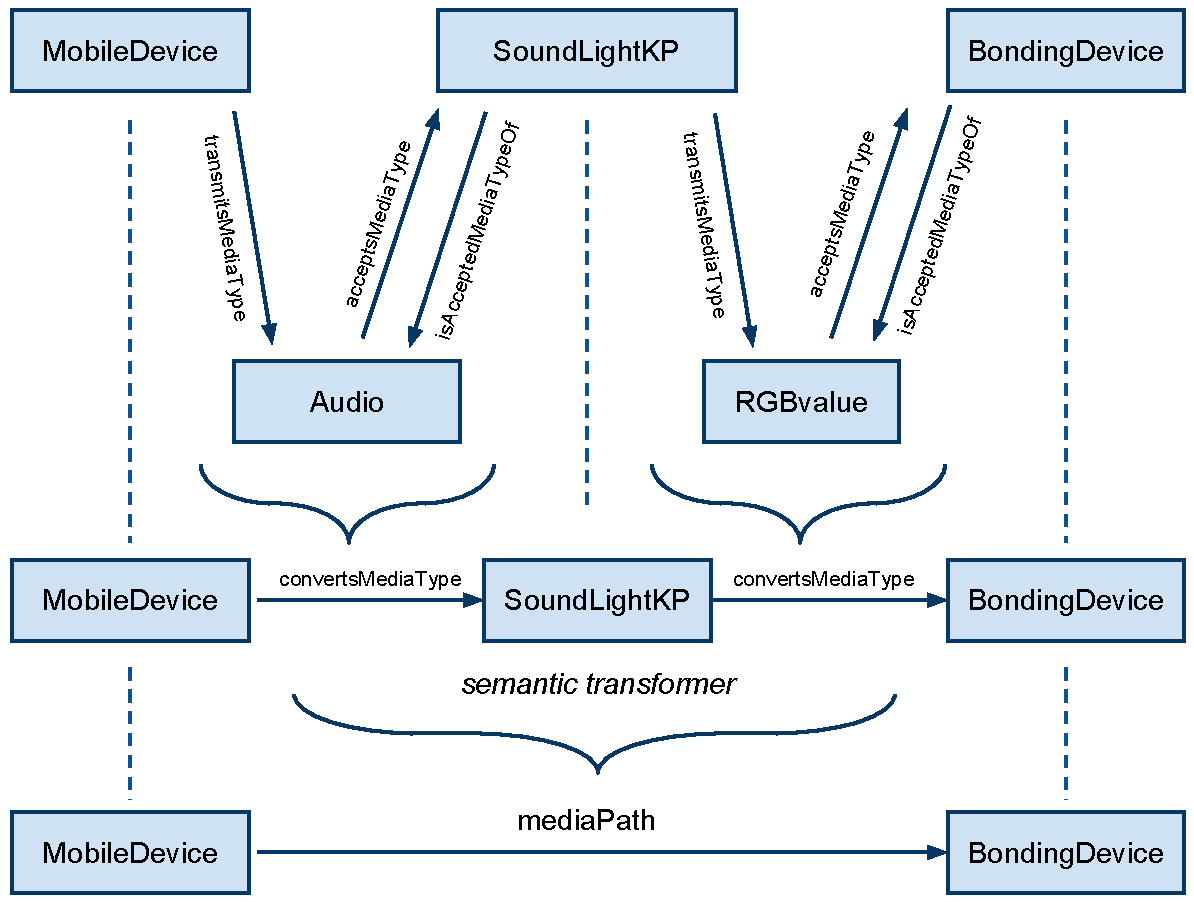
\includegraphics[width=250px]{SemanticTransformers}
\caption{Inferring the media path}
\label{mediapath}
\end{figure}

This allows us to match media types between smart objects. We can then infer a \textit{media path} between the mobile device and the Bonding Device with the Sound/Light KP acting as a semantic transformer using another property chain:

\begin{quote}
convertsMediaType~\ensuremath{\circ}~convertsMediaType~\ensuremath{\sqsubseteq}~mediaPath
\end{quote}

\noindent To then determine the media source itself we use \ac{SWRL}\footnote{http://www.w3.org/Submission/SWRL/}, as the expressivity of \ac{OWL} does not allow for inferring the media source if there are more than one \texttt{convertsMediaType} relationship linked to the lighting device:\marginpar{This \ac{SWRL} implementation was later replaced using another Semantic Web technology called SPIN, detailed in Chapter \ref{OntologyEngineering}.}\\


\texttt{\scriptsize
convertsMediaType(?x1,?x2)~\ensuremath{\wedge}~convertsMediaType(?x2,?x3)~\ensuremath{\Rightarrow}~mediaSource(?x3, ?x2)}

The media source is the semantic transformer, \texttt{?x2}, while the media path is between the two smart objects, \texttt{?x1} and \texttt{?x3}. The \texttt{mediaSource} relationship is thus inferred from the smart object to the semantic transformer. We can also infer whether a device is a semantic transformer or not using:


\begin{minted}{turtle}
Class: SemanticTransformer

    EquivalentTo:
        (canAcceptMediaTypeFrom some SmartObject) and
        (convertsMediaType some SmartObject)

    SubClassOf:
        SmartObject
\end{minted}


The end result is that the lighting device responds to the mobile device's media events (based on the Semantic Connections \texttt{connectedTo} relationship), but uses the Sound/Light KP as a media source for generating dynamic lighting. The \texttt{connectedTo} relationship between the mobile device and the lighting device should only be possible if a media path exists between the two devices. Figure \ref{mediapath} illustrates the entire process of inferring the media path from the original media type definitions.
%end africon

If the reasoner infers a media path between two smart objects, it does not mean that they are automatically connected -- it means that a connection is possible. The user can view this connection possibility using either the Connector device or the Spotlight Navigation device, and then establish the connection if necessary.

\subsection{Device states}

Interaction events (Chapter \ref{EventModelling}) cause device state changes. Most of the developers that worked on the Smart Home Pilot preferred to describe their smart objects in terms of the device states, and also shared these device states with other smart objects using the SIB. The current state of the smart object was defined using the \texttt{sofia:isInState} property:

\begin{minted}{turtle}
	conante:spotlight1 sofia:isInState "projecting" .
	sofia:nflKP1234 sofia:isInState "lightingON" .
	sofia:nflKP5678 sofia:isInState "lightingOFF" .
	sofia:presenceKP1234 sofia:isInState "Away" .
	sofia:presenceKP5678 sofia:isInState "Present" .
\end{minted}

These smart objects were all simple two-state devices, where the device state was indicated using a text field. Note that \texttt{conante:spotlight1} used the absence of \texttt{sofia:isInState} property to indicate that it was not projecting. This statement is valid with a \ac{CWA}, the presumption that that what is not currently known to be true, is false. The programmer that created this state description is well versed in the Prolog programming language, which makes the \ac{CWA}. \ac{OWL}, on the other hand, operates under the \ac{OWA}. With \ac{OWA}, we assume that new information can become available at any time, so that we cannot draw conclusions based on the assumption that all information is already available \cite{Allemang2011}. We can use the ontology to restrict how state descriptions are reported, forcing smart objects to report their current state at all times.\marginpar{The \ac{OWA} is also discussed in Section \ref{CardinalityRestrictions}.}




\section{Evaluation}
\label{D2Evaluation}
A number of issues were identified during the evaluation of the Smart Home pilot. In the Smart Home pilot there were two locations connected via a permanent semantic connection between the lighting devices. What if Sofia were to play a song in her room --- will the same song play back at the home of Mark and Dries? If this is the case, we clearly need to introduce a notion of directionality in the semantic connections. This issue is addressed in Design Iteration III in the next chapter.

The Pellet reasoning engine with \ac{SWRL} rules proved to be a performance bottleneck in the system. For example, Pellet took about 3 seconds to infer 107 statements.\marginpar{In one instance, a \ac{SWRL} rule took up to 28 seconds to execute.} TopBraid Composer's TopSPIN reasoning engine supports \ac{SPIN} rules and \ac{OWL} 2, so it was tested as a possible alternative. The TopSPIN engine with OWL 2 RL/RDF Rules took less than a second to infer 10 491 triples. By using a hashmap to store our inferred triples, we were able to improve performance even further. Some of the inferred triples were redundant inferences -- by using a hashmap we were able to reduce the number of inferred triples on startup from 10 491 to 5 122, eliminating redundant triples.

A more formal performance evaluation as well as a user evaluation of the ontology, both of which were performed on the work done in this iteration, is discussed in Chapter \ref{Evaluation}.

% - Evaluation: 
% 	- How to define dim level, InUse state. 
% 	- If song 1 is playing in location 1, and song 2 is in location 2, which gets preference? -> directionality needed
% 	- Early SIB performance measurements (22/03/11, also GDocs)
% 	- Comparing SPIN+Pellet to SPIN+OWL2RL/RDF Rules:
% 		- Pellet takes 3 seconds to realize 107 elements
% 		- OWL2RL/RDF Rules takes less than a second to infer 11 361 triples
% 		- OWL2R/RDF Rules performance further improved by storing inferred triples in hashmap (see implementation). Also reduced number of inferred triples on startup form 10 491 to 5 122
		
		
\section{Discussion \& Conclusion}
\label{D2Discussion}
%\subsection{Implementation issues}

Modelling constraints in the ontology is done using \emph{restrictions}.  When modelling concepts in an \ac{OWL} ontology, restrictions are defined either as part of \texttt{rdfs:subClassOf} or as part of \texttt{owl:equivalentClass}. There is a subtle difference, and it has to do with \emph{necessary and sufficient conditions}.

When we have necessary and sufficient conditions (also known as \emph{if and only if} and denoted as $ \equiv $, $ \leftrightarrow $ or $ \Leftrightarrow $), the \texttt{owl:equivalentClass} restriction (denoted as $ \equiv $) is used. When we only have necessary conditions, the \texttt{rdfs:subClassOf} restriction (denoted as $ \sqsubseteq $) is used. \emph{Necessary and sufficient} means that the restriction is sufficiently constrained that only individuals belonging to that class will be classified as such.\footnote{In the Prot\'eg\'e ontology editor these are also called \emph{defined classes}.} An example is shown in Section \ref{SemanticMatching}. \marginpar{An \ac{OWL} reasoner follows a bottom-up approach, where new information is inferred from asserted facts, compared to a theorem prover that starts from its goal.}



% Idempotency is the property of being able to perform the same action twice or more times in sequence, and end up with the same result as if the action was performed once. In the triple store, defining a smart object or interaction primitive is idempotent as long as the definition  doesn't change on the triple-level. The idempotency of interaction events depends on whether a new timestamp is used when inserting the event into the triple store.
% 
% 
% ==TODO Idempotence
% Idempotence is the property of being able to perform the same action twice or more times in sequence, and end up with the same result as if it was performed once. As an example, consider the different HTTP methods:
% 
% \begin{itemize}
% 	\item PUT - uploads a representation of a specified resource
% 	\item DELETE - deletes the specified resource
% 	\item POST - can either update an existing resource or create a new resource
% \end{itemize}
% 
% PUT and DELETE are idempotent, while POST is not. In our case, creating a new interaction event is not idempotent, but inserting the same triple twice is. In the triple store, defining a smart object or interaction primitive is idempotent as long as the definition  does not change on the triple level. The idempotence of interaction events depends on whether a new timestamp is used when inserting the event into the triple store.



The ontology supports the description of interaction data generated by interaction devices and sensors. Additionally, it shows that an interaction primitive may trigger an interaction event or a state change that may need to be specified in more detail by a more application-specific ontology. That is to say, this ontology may also be used to perform semantic mapping from the interaction data to user goals and/or available services \cite{Niezen2010}. Any additional information related to the smart object may be added by extending the schema defined in the Semantic Interaction Ontology. 

Another advantage of the ontology described in this section is that opens up the way to context-based interaction device reconfiguration. For example, if a Context Monitor application recognises a situation where the \texttt{PhoneRockerSwitch} should no longer control the volume, but adjust the level of lighting instead, the triple could be modified accordingly. Just such a simple change would implement a behaviour that adapts to the situation.

Context-dependent functionality changes of a control may not necessarily be a desirable feature and there is a long standing discussion on whether or not to allow for such behaviour in user interface research. It should however be noted that we only consider context-dependent meaning change with generic interaction primitives, that in itself do not have a specific, function related meaning (and might already being used for different functions, like the rocker switch in the example). Additionally, the re-mapping is only considered for those interaction elements with compatible transformational properties, e.g. the rocker switch may only be mapped to other \texttt{AdjustLevel} transformations, and not to \texttt{Start/Stop}. The specified range measures are used to control the re-mapping between a interaction primitive and an interaction event, in a similar way that the input and output domains of \cite{MacKinlay1990} are used to control the expressiveness between an input device and its application parameter. 

The question then becomes how to inform the user of the remapping in a user-friendly way. In the next chapter we consider the different types of feedback that can be used. Besides automatic context-dependent functionality changes of controls, we especially consider user-initiated re-mapping of controls. By enabling users to make associations, or semantic connections \cite{VanderVlist2010} between devices or interaction elements and devices, users can express their intentions in terms of mapping controls between devices \cite{Niezen2010}. 

% While most of the issues discussed in this paper also applies to user interaction in general, 
% the way in which interaction events and interaction primitives are distributed between multiple devices makes our work very applicable to ubiquitous computing environments. Semantic mapping between interaction primitives and interaction events on different devices is also supported.
% 
% The use of interaction primitives to model the essential elements of user interaction is currently being implemented by various project partners, and up until now seem promising. A thorough evaluation and validation is part of our next steps, as well as integration of the introduced concepts into the SOFIA core ontology or application- or domain-specific ontologies.
%end africon

% Spotlight Navigation and the Connector are two alternative user interface approaches to configuring ubiquitous computing infrastructure. Although we cannot directly compare the mental models elicited during the user experiment, which would have asked for a more controlled setting (e.g. having the same setup and having an equal number of participants for both treatments), we did make some interesting observations.

% The most striking difference between the way users described the setup was the perception of the users that the Connector was part (if not the central part) of the system, while the Spotlight Navigation was often considered outside of the system. We hypothesise that this is due to the different roles that the Spotlight Navigation and the Connector have in the interaction with the connections. The Connector is used to conceptually ``carry'' the content between the two devices and in itself represents the relation between these two artefacts. The Spotlight Navigation is, in contrast, perceived as a ``remote control'' that visualises the connections in physical space. This might lead the users to conclude that the projected lines are the connections, directly between the devices, and leave the Spotlight Navigation itself outside of this network.

%begin S3E
Judging from the experience of implementing the semantic transformers, the approach of using them to solve interoperability problems appears promising. Using the Semantic Media Ontology, we were able to define a smart object in terms of the media types it accepts and transmits. Based on these descriptions, semantic transformers can be used to transform media types in order to enable information exchange between devices that would normally not be able to communicate. With only a minimal set of device capabilities described, the system is able to perform self-configuration using semantic reasoning.
%end S3E

%begin africon
Even though the Semantic Interaction Ontology describes parts of a \texttt{SmartObject}, it does not fully describe all the properties and capabilities of the smart object. It only describes its interaction-related properties. Particularly it defines the \texttt{SmartObject} interaction primitives and means of identification. In the next chapter, while describing the next iteration, we will focus on expanding the possibilities of describing a device's functionality and capabilities.



\chapter{Design Iteration III}
\label{DesignIteration3}

\begin{flushright}{\slshape    
Making everything visible is great when you only have twenty things. \\
When you have twenty thousand, it only adds to the confusion.} \\ \medskip
    ---  Don Norman \cite{Norman1999}
\end{flushright}


The goal of the final iteration was to extend the scenarios developed in the previous iterations to a new domain, while still making use of the smart objects and concepts that have been developed thus far. This would allow for testing the general applicability of the concepts and techniques, while still being able to reuse some of the devices we have already developed.

\section{Requirements}

The use case scenario in this iteration revolves around a person's evening routine before falling asleep. It is a cross-domain scenario that extends the media domain into the sleep domain, and enables the exchange of different types of information. The domain of sleep was chosen for several reasons:

\begin{itemize}
\item Sleep is important for physical and mental well-being --- an important application area of our research group at TU/e.
\item The sleep domain is targeted by a number of recent \ac{IoT} devices that record and share data and can be accessed through their \acp{API}.
\item 	The sleep domain allows us to reuse some of our existing work on media sharing and lighting, extending it into a new domain.
\end{itemize}

In the fitness and sleep domains there are a plethora of devices that are well-known to the \ac{IoT} community but that are not interoperable, such as:

\begin{itemize}
	\item the Withings WiFi body scale\footnote{http://www.withings.com/en/bodyscale}, that transfers body weight wirelessly to a computer or mobile device,
  	\item the Fitbit\footnote{http://www.fitbit.com/} and Nike FuelBand\footnote{http://www.nike.com/fuelband/} fitness monitors, that track activities using a built-in accelerometer, and
	\item the Zeo sleep monitor\footnote{http://www.myzeo.com}, that records sleep cycles using a head-mounted sensor.
\end{itemize}
 

Existing software applications targeted at these devices visualise the data coming from these devices. Our goal is to enable serendipitous interoperability, and we are interested in seeing what will happen when the data and capabilities are shared between these devices. For example, we could use the data coming from a sleep monitor to to change the behaviour of a light in the room, or the alarm on a mobile phone. We distinguish between a number of subdomains within the area of well-being, as shown in Figure \ref{Wellbeing}.

\begin{figure}[bth]
\begin{center}
	\digraph[scale=0.65]{Wellbeing}{
		node [shape=plaintext, fontsize=16];
		Wellbeing [label="Well-being"];
		{rank=same; Social; Physical; Mental}
		{rank=same; Fitness; Sleep}
		Wellbeing -> Social [arrowhead=None];
		Wellbeing -> Physical [arrowhead=None];
		Wellbeing -> Mental [arrowhead=None];
		Physical -> Fitness [arrowhead=None];
		Mental -> Sleep [arrowhead=None];
	}
	\caption{Sub-domains of well-being}
	\label{Wellbeing}        
\end{center}
\end{figure}

Several devices were used in Iteration III, including:

\begin{itemize}
	\item an Android smart phone -- Samsung Nexus S;
	\item an internet radio -- Logitech Squeezebox Radio;
	\item the lamp from Section \ref{Lamp};
	\item a sleep monitor -- Zeo Sleep Manager; and 
	\item an Android tablet -- Samsung Galaxy Tab 10.1 WiFi.
\end{itemize}

We purposefully did not define a narrative for this design iteration, to refrain from only implementing the functionality described in the narrative. Instead, we looked at the meaningful ensembles we could create with the devices, attempting to allow for \emph{emergent functionalities} to surface by sharing device capabilities and interaction events.

The design iteration was implemented in the master bedroom of the Context Lab of TU/e, a lab with a setting that resembles a real home. Implementing the setup in an environment that allowed us to see its behaviour and implications in a realistic setting, gave insights that are regarded more valuable than obtained when building a setup on for example one's office desk. 


\section{Ontology design}
\label{OntologyDesign3}

In this iteration the earlier ontologies were consolidated into a single ontology. This helps make the ontology more manageable and removes the ``cruft'' of legacy statements that build up over time. 

The first design decision of this iteration was to introduce the notion of directionality. This gives additional meaning to the devices, which now need to be modelled as \emph{sources}, \emph{sinks} or \emph{bridges}. A music player is an example of a smart object that acts as a source when connected to a speaker, which in turn acts as a sink. When transitivity is introduced, a smart object can act as both a source and sink, which we define as a bridge. For example, consider the case where the speaker is connected to another speaker, which then also plays back the same music. The first speaker then acts as a bridge.

We can infer that a smart object is a sink using\\

\noindent Sink~\ensuremath{\equiv}~SmartObject~\ensuremath{\sqcap}~(functionalitySink~\ensuremath{\exists}~Functionality)\\\marginpar{See Table \ref{syntaxTable} on page \pageref{syntaxTable} for more details on the symbols and syntaxes used in this thesis.} 

where the symbol \ensuremath{\exists} is used to denote the existential restriction that \texttt{functionalitySink} is some kind of \texttt{Functionality}. A bridge is inferred using\\

\noindent Bridge~\ensuremath{\equiv}Sink~\ensuremath{\sqcap}~Source\\ 

A semantic transformer is a virtual component that is not physically addressable and is therefore not considered to be a smart object. However, it is a bridge, as it acts as both a source and a sink. A smart object is a physical object first, with a digital representation added later.\marginpar{Semantic transformers were first introduced in Section \ref{OntologyDesign2} and are discussed in more detail in Section \ref{SemanticTransformers}.}

Other areas where the ontology was improved include the modelling of device capabilities (Chapter \ref{DeviceCapabilityModelling}) and the modelling of events (Chapter \ref{EventModelling}). These improvements are discussed in more detail in the relevant chapters. 


%\section{Setting the time}
%It is reasonable to assume that modern networked devices will synchronize their clocks to a time server to display the actual time. Unfortunately, this is not the case. In our test setup, the internet radio synchronizes its clock with the local or remote server that it is connected to. The Android phone synchronizes its clock when it is connected to the GSM network 


\section{Device modifications}

In this iteration, we reused both the ambient lighting system from Section \ref{Lamp}, as well as the Connector object from Section \ref{Connector}. For the Squeezebox radio and Android devices new \ac{KP} software was developed.

\subsection{Squeezebox radio}

\begin{figure}
\centering
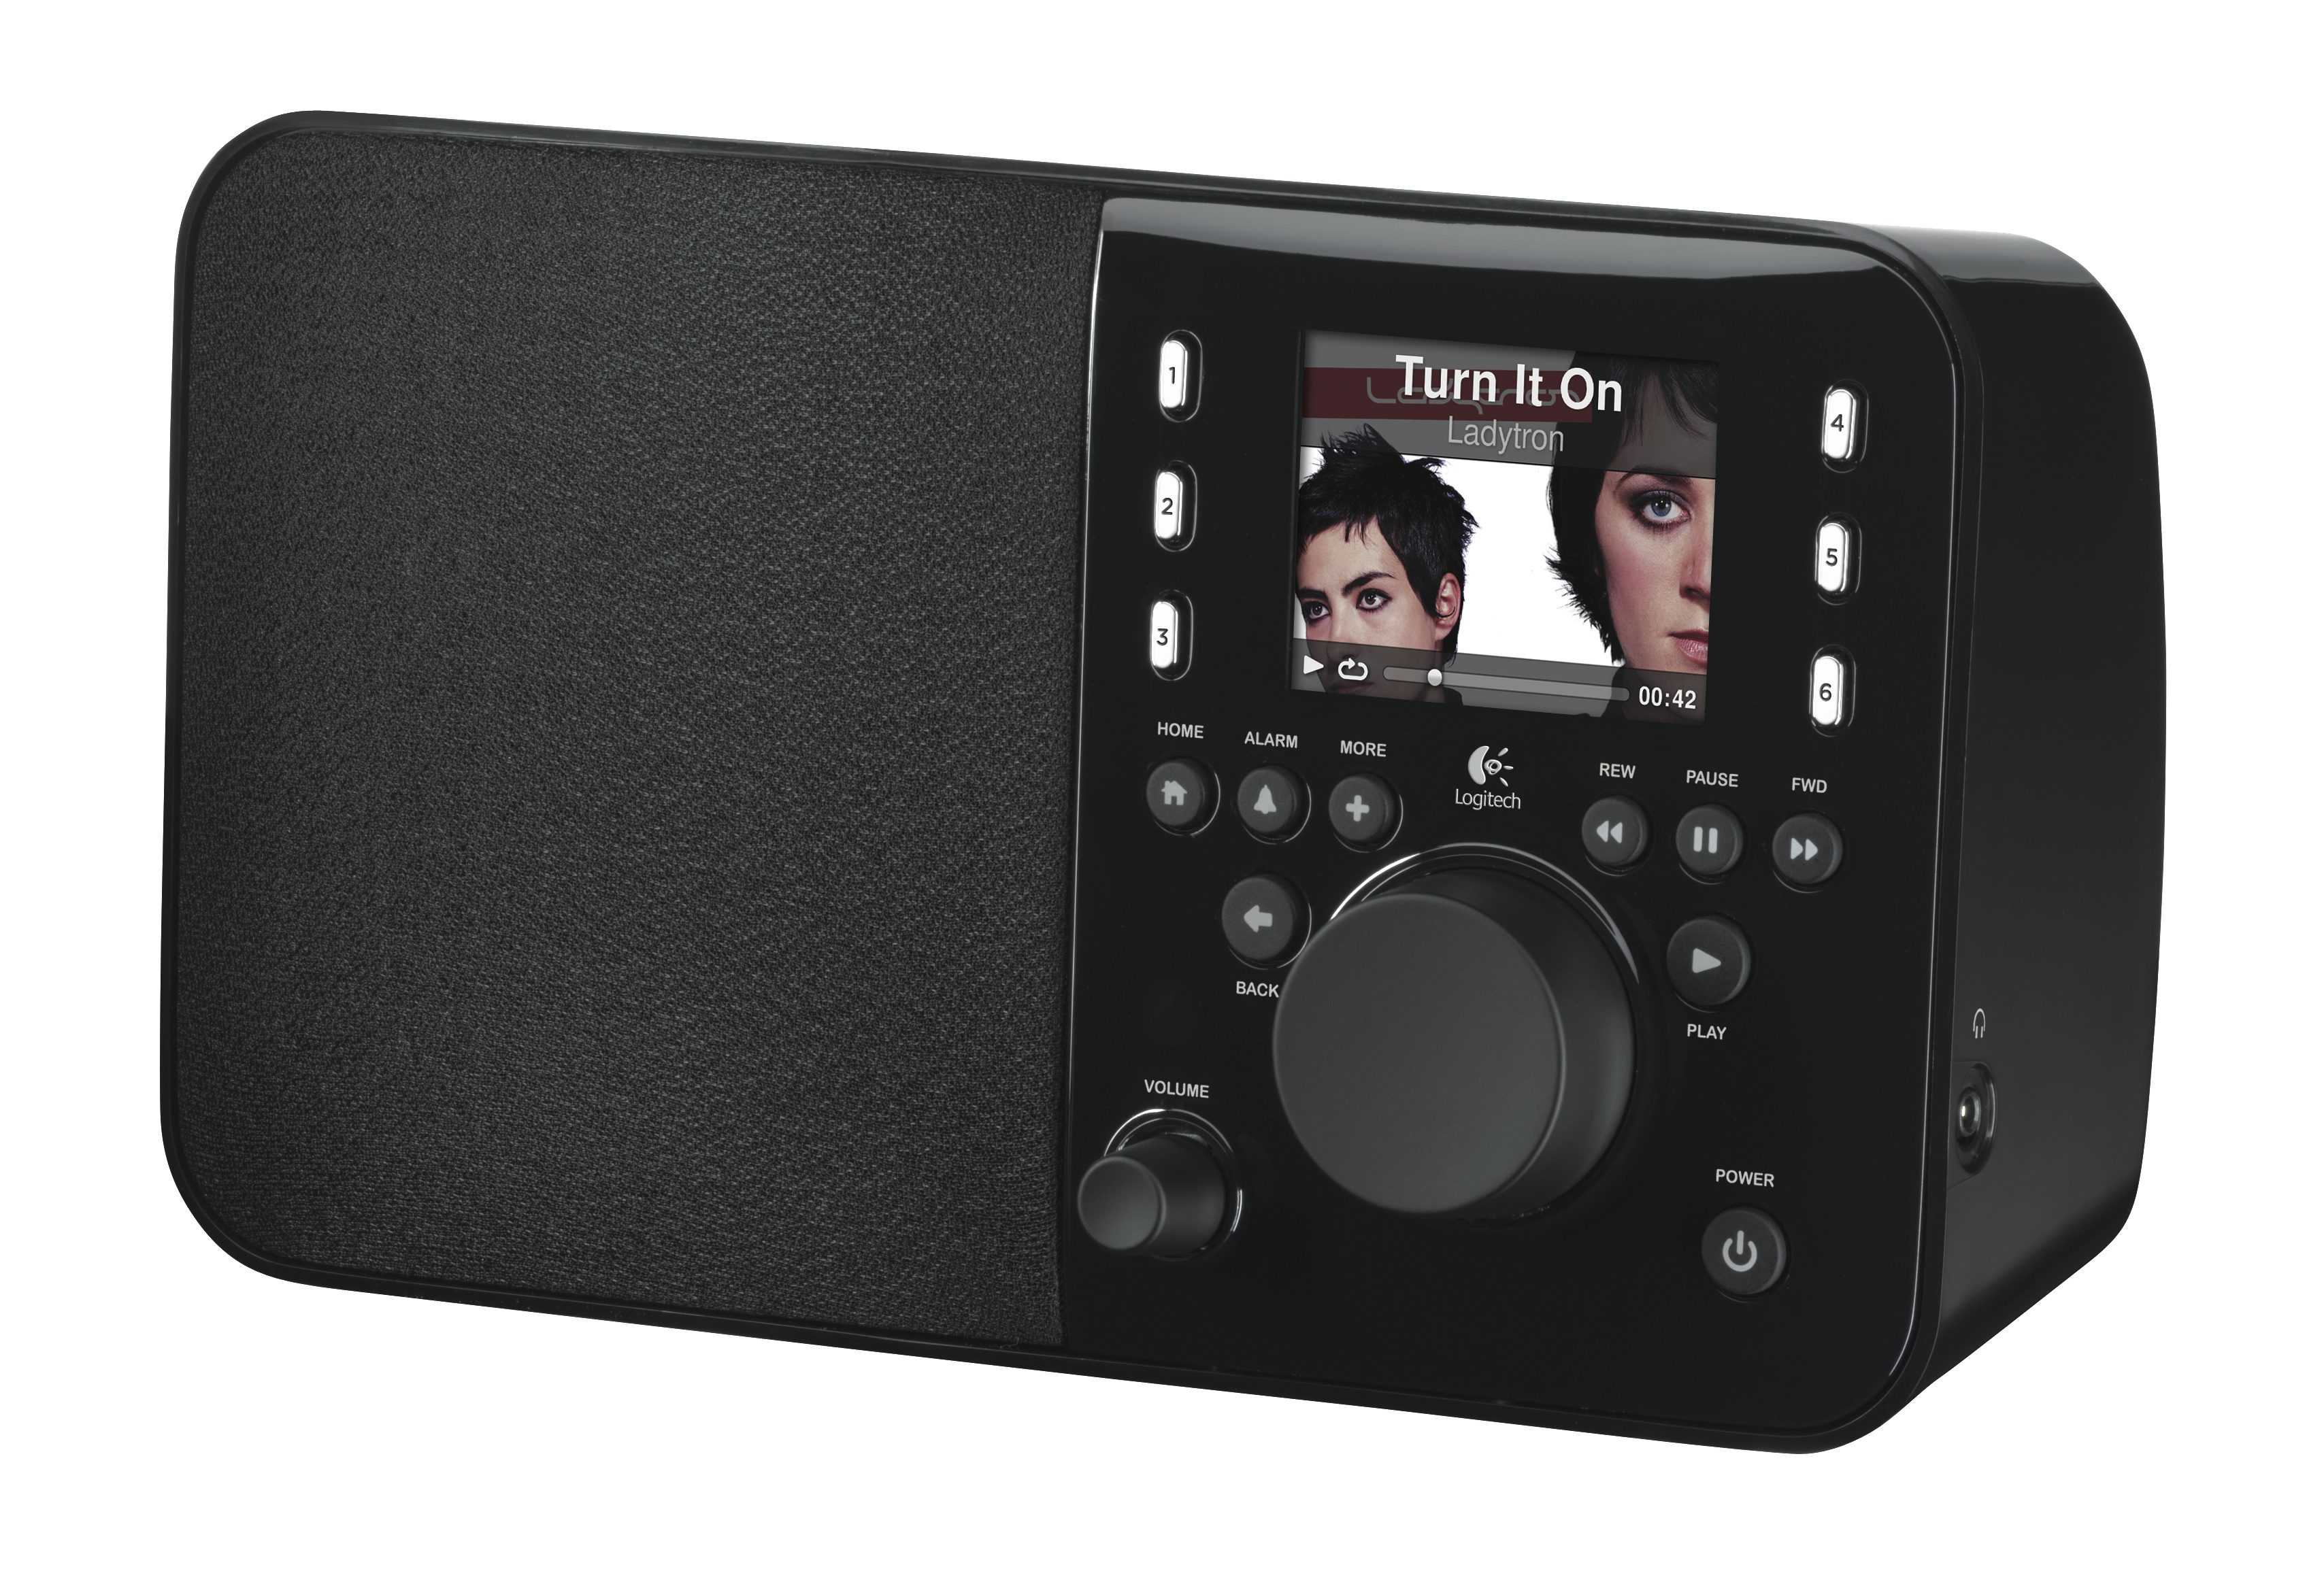
\includegraphics[width=300pt]{squeezebox}
\caption{Logitech Squeezebox Radio}
\label{squeezebox}
\end{figure}

The Squeezebox radio, shown in Figure \ref{squeezebox}, can be controlled via a Telnet interface over WiFi.\footnote{On Squeezebox Server, the interface documentation is available from \texttt{Help}~$\Rightarrow$~\texttt{Technical Information}~$\Rightarrow$~\texttt{The Squeezebox Server Command Line Interface} }. 
For example, the accepted parameters for setting an alarm are shown in Table \ref{SetAlarm}.

\begin{table}
    \myfloatalign
  \begin{tabularx}{\textwidth}{Xl} \toprule
    \tableheadline{Parameter} & \tableheadline{Description} \\ \midrule

    \texttt{dow} & Day of week (0 -- 6, starts on Sunday) \\
	\texttt{time} & Time since midnight in seconds \\
	\texttt{repeat} & 1 or 0 \\
	\texttt{volume} & 0 -- 100 \\
	\texttt{url} & Squeezebox Server \ac{URL} of alarm playlist \\
	\texttt{id} & The ID of an existing alarm (optional for new alarms) \\
    \bottomrule
  \end{tabularx}
  \caption{Accepted parameters for Squeezebox \texttt{alarm} Telnet command}  \label{SetAlarm}
\end{table}

On startup, the Squeezebox \ac{KP} connects to the smart space, registers the capabilities of the device, checks for existing connections and listens for new connections. It also subscribes to new system events.\marginpar{System events are discussed in more detail in Chapter \ref{OntologyEngineering}.} It then connects to the Squeezebox device via the Telnet-over-WiFi interface, subscribes to new events generated by the device and enters an event loop.


When a new alarm is set on the device, the \ac{KP} converts the date and time to \ac{XSD} format and generates a new \texttt{AlarmSetEvent}. When an alarm is triggered, an \texttt{AlarmAlertEvent} is generated. If the alarm is dismissed on the device, an \texttt{AlarmEndEvent} is generated. When an alarm is deleted, an \texttt{AlarmRemoveEvent} is generated.

When an \texttt{AlarmSetEvent}, \texttt{AlarmRemoveEvent}, \texttt{AlarmEndEvent} is received from another device, the corresponding action is performed on the device. \marginpar{Media events were introduced in Section \ref{MusicPlayerKP}.}The device also responds to media events like \texttt{PlayEvent}, \texttt{PauseEvent} and \texttt{PlayEvent}.


\subsection{Android mobile devices}

\begin{figure}
\centering
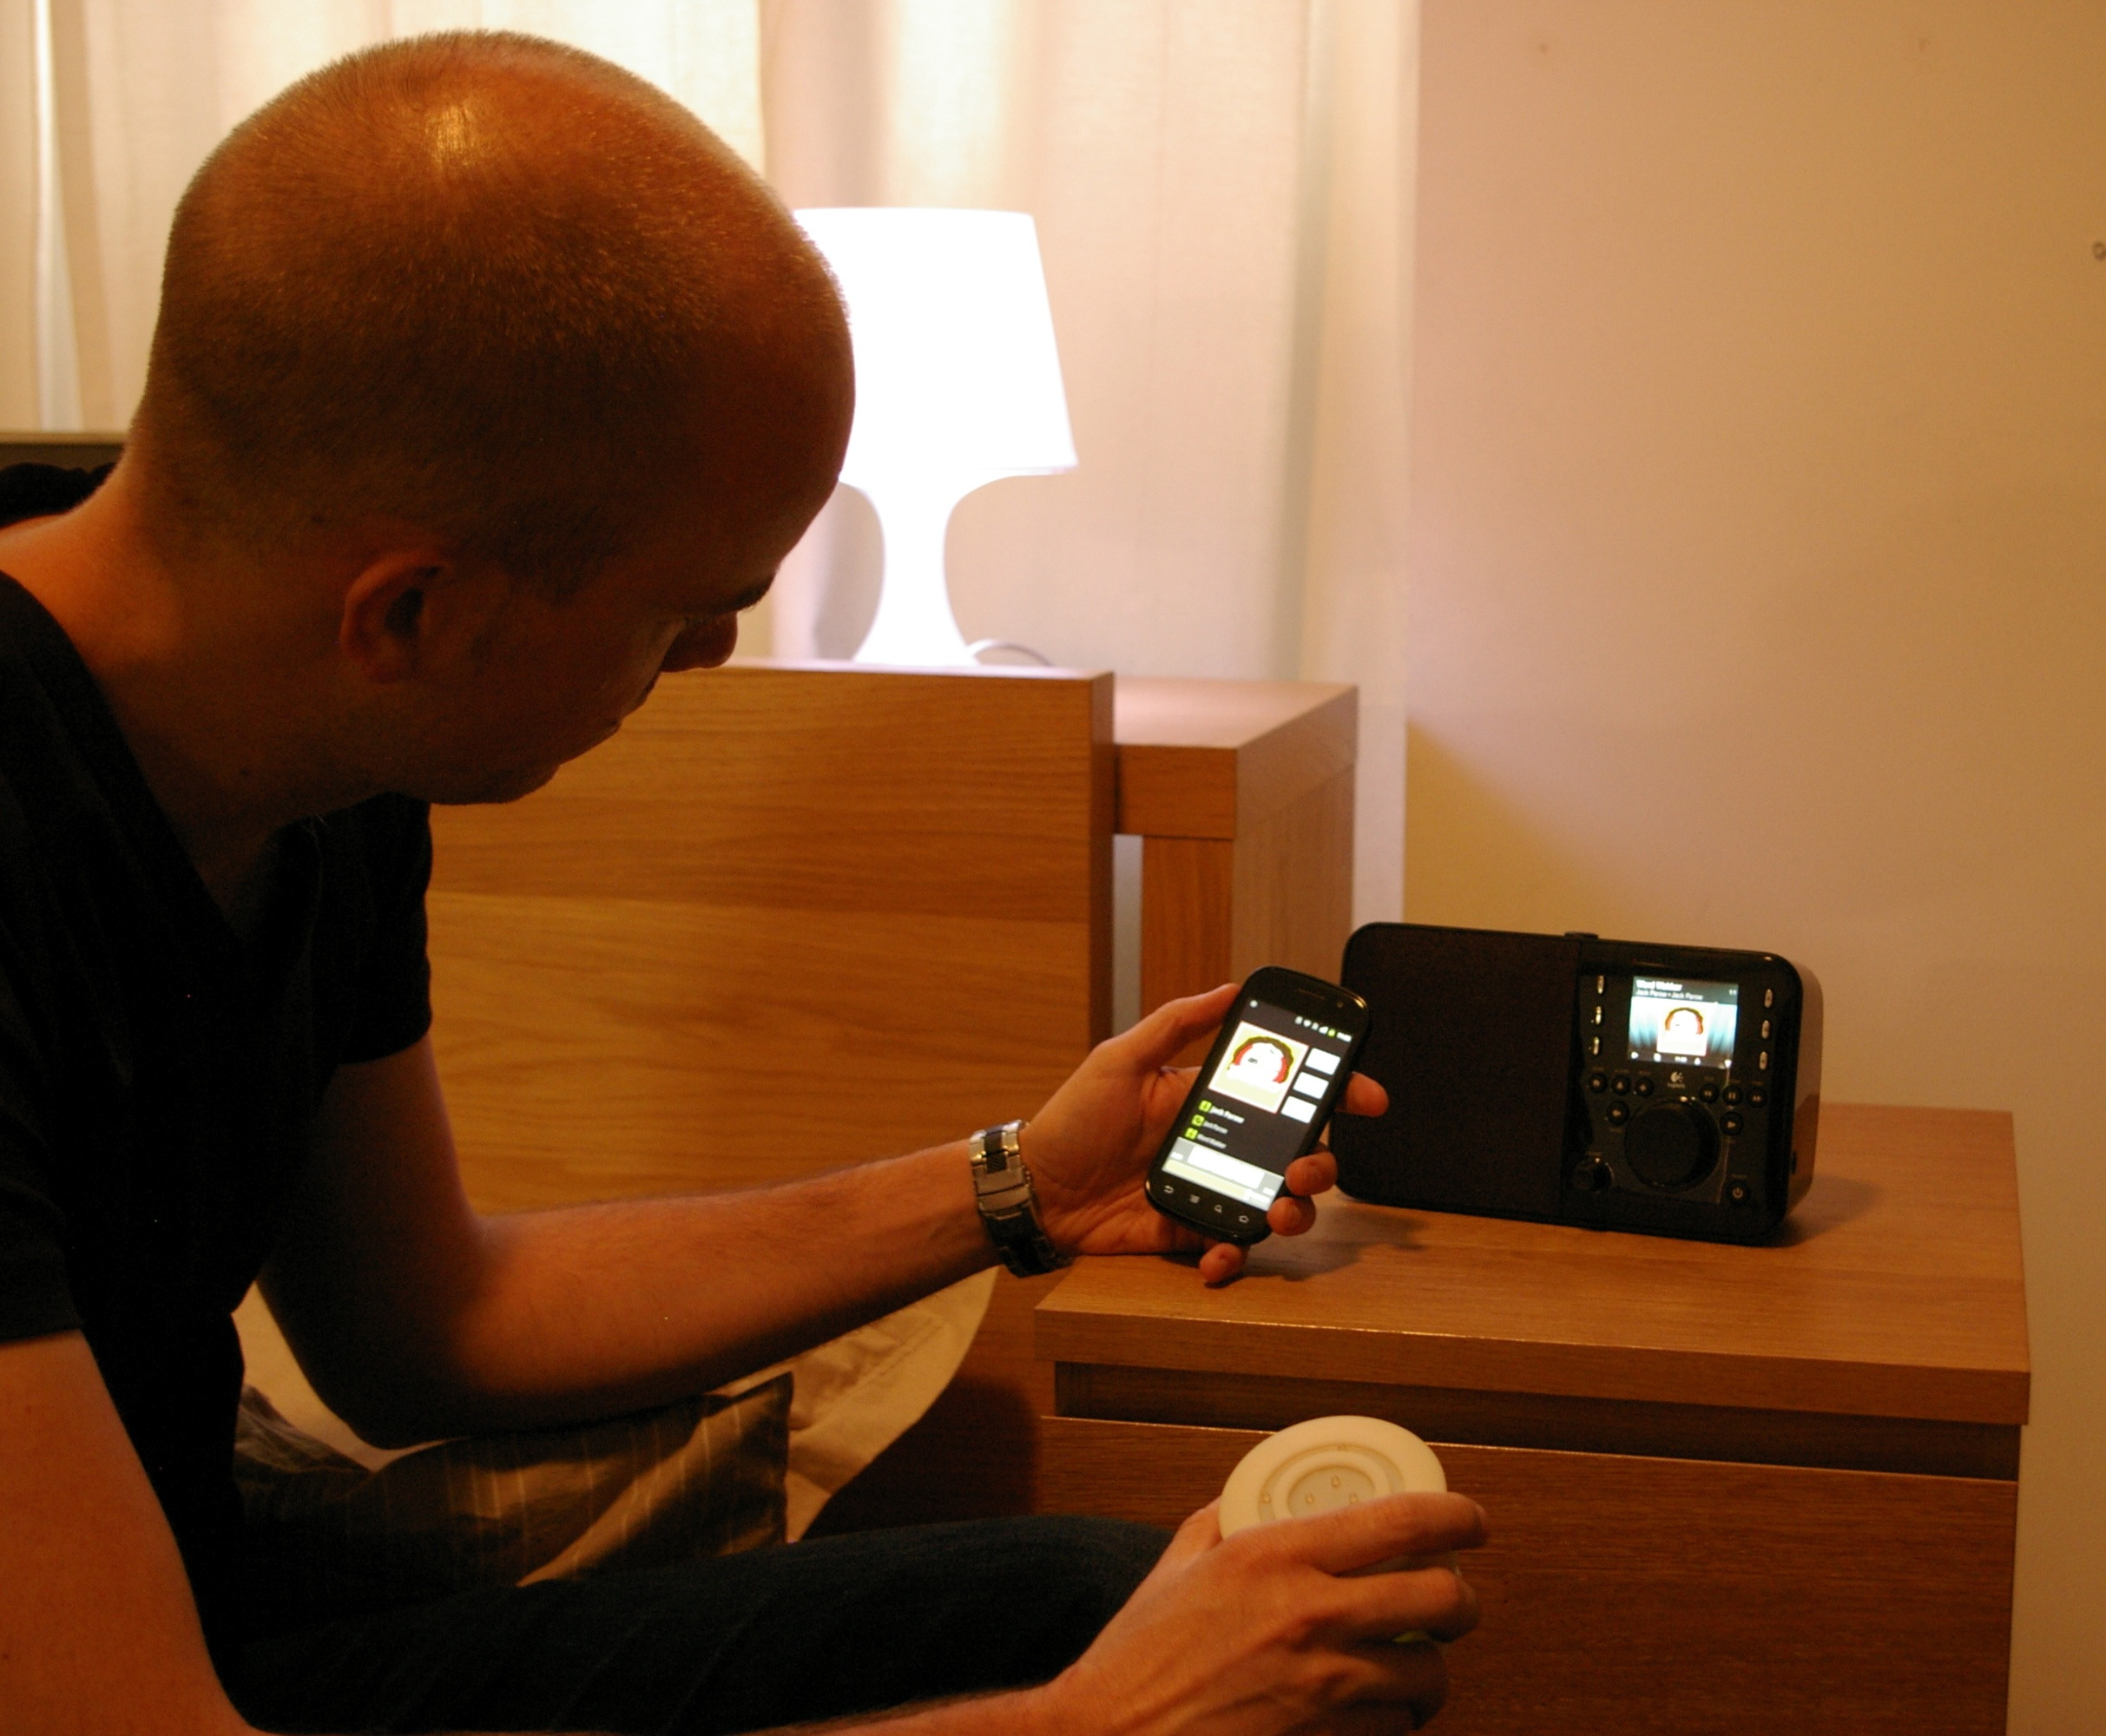
\includegraphics[width=300pt]{nexus}
\caption{Playing music from the phone on the Squeezebox radio}
\label{nexus}
\end{figure}

\marginpar{The \ac{KP} developed for the Android devices was tested on both the Google Nexus S phone and the Samsung Galaxy Tab.}
To improve software reuse and not reinvent the wheel, we wanted to make use of the stock applications on the phone, like the Clock app and the Music app (shown in Figure \ref{nexus}), instead of developing our own. On Android, it is possible to run a service as a background process that listens for events generated by other applications. A \emph{broadcast receiver} listens for \emph{broadcast intents}, which are public intents broadcast from activities to registered receivers. A receiver registers for a broadcast intent by listing it in its intent filter in the manifest file.\marginpar{Android activities run inside applications.} Broadcast intents sent by Android applications can be received by all other applications, which is done by creating a broadcast receiver. 

When the alarm is triggered in the alarm app on the mobile phone\marginpar{The alarm app on the Google Nexus S phone is called \texttt{DeskClock} and was developed by Google. There also exists a version for earlier Google phones called \texttt{AlarmClock}.}, a \mint{java}|com.android.deskclock.ALARM_ALERT| broadcast intent is generated. 

A broadcast receiver handles such an intent using 

\begin{minted}{java}
@Override
protected void handleBroadcastIntent(Intent broadcastIntent) {
	String action = broadcastIntent.getAction();
	if(action.equals("android.intent.action.ALARM_ALERT")) {
		addEvent("AlarmAlertEvent");
	}
}
\end{minted}
	
Note that this intent is not supported by all Android devices, as different devices may have different default alarm applications. It did, however, work on both the Google Nexus S phones and Samsung Galaxy tablets that we tested. To determine when an alarm was changed, we made use of the \mint{java}|android.intent.action.ALARM_CHANGED| broadcast intents. It is also possible to read the next alarm that will triggered from the system settings, using \mint{java}|System.Settings.NEXT_ALARM_FORMATTED| To determine if a song is being played using the Android Music app, we used the \mint{java}|com.android.music.playstatechanged| broadcast intent.

\marginpar{The Lighted Greenroom pattern was introduced by Komatineni et al. \cite{Komatineni2011} to simplify interacting with the Android wake lock.}
We used a Lighted Greenroom \cite{Komatineni2011} pattern to launch a long-running service from a broadcast receiver, without the operating system throwing an \ac{ANR} message. \ac{ANR} specifies a 10-second response limit for a broadcast receiver, after which it is deemed unresponsive. By launching a separate service that handles generation of events based on broadcast intents, we have a workaround to this problem. This allows us to listen for broadcast intents from applications like the music player and the alarm clock.
%(e.g. \texttt{com.android.music.playstatechanged}) and the alarm clock (\texttt{android.intent.action.ALARM\_CHANGED})

\subsection{Wakeup experience service}

In the sleep use case, music can be shared between the smart phone and the internet radio. Alarms can be shared between the phone and the internet radio, the internet radio and the lamp as well as the phone and the lamp. Because the lamp has only \texttt{LightOn/LightOff} and \texttt{AdjustLevel} capabilities, the most basic functionality of the lamp responding to an \texttt{AlarmEvent}, would be to turn on at the time that the event occurs. However, a wakeup service can be connected that \emph{transforms} an \texttt{AlarmSetEvent} into a wakeup experience, sending a sequence of \texttt{AdjustLevelEvents} to the lamp. This wakeup service then functions as a semantic transformer, transforming one type of value into another in a meaningful way. Semantic transformers are virtual entities and therefore they do not have a physical presence, in contrast to smart objects that must have a physical representation. Therefore, the use of a semantic transformer is automatically inferred based on its capabilities, as it cannot be physically connected to other devices by the user. 

To create a wakeup service, an \texttt{AlarmSetEvent} would have to trigger an \texttt{AdjustLevelEvent} event with a \texttt{dataValue} that increases from 0 to 100 over a period of 30 minutes \emph{before} the alarm sounds. Another requirement is that it should work with any light and any alarm in the smart environment. 

%The Wakeup \ac{KP} is a type of semantic transformer, and transforms \texttt{AlarmSetEvents} into a series of \texttt{IncreaseLevelEvents} (which is a sub-property of \linebreak \texttt{AdjustLevelEvents}). However, this happens in a way that is designed by the developer of the \ac{KP} and as such, can be seen as a (digital) service. 

This wakeup service has similar functionalities as a Wakeup Light (e.g. as sold by Philips\footnote{http://www.philips.co.uk/c/wake-up-light/38751/cat/}) which means it starts increasing its light level over a 30 minute time-period, reaching full intensity (as calibrated) at the set alarm time. The semantic connection between the phone's alarm and the dimmable light is an example of how such a connection can have emerging functionality, which does not exist without the connection and the wakeup service.  

This opens up many possibilities for users, as they may connect other lights, and potentially even other devices such as a networked thermostat, to either the alarm or the dimmable lamp, creating their own wakeup experience. Whether such emerging functionalities are possible obviously depends on the way the smart objects are implemented. For example in our implementation, the dimmable lamp is described as a sink, which means it is only capable of accepting input. If it was described as a source as well, sharing for instance its on/off state or its current light value, it could act as a bridge and allow for more interesting configurations. %Users may also connect the sleep monitor as an alarm source, helping them to wake up at the right time in their sleep cycle.

\begin{figure}
\centering
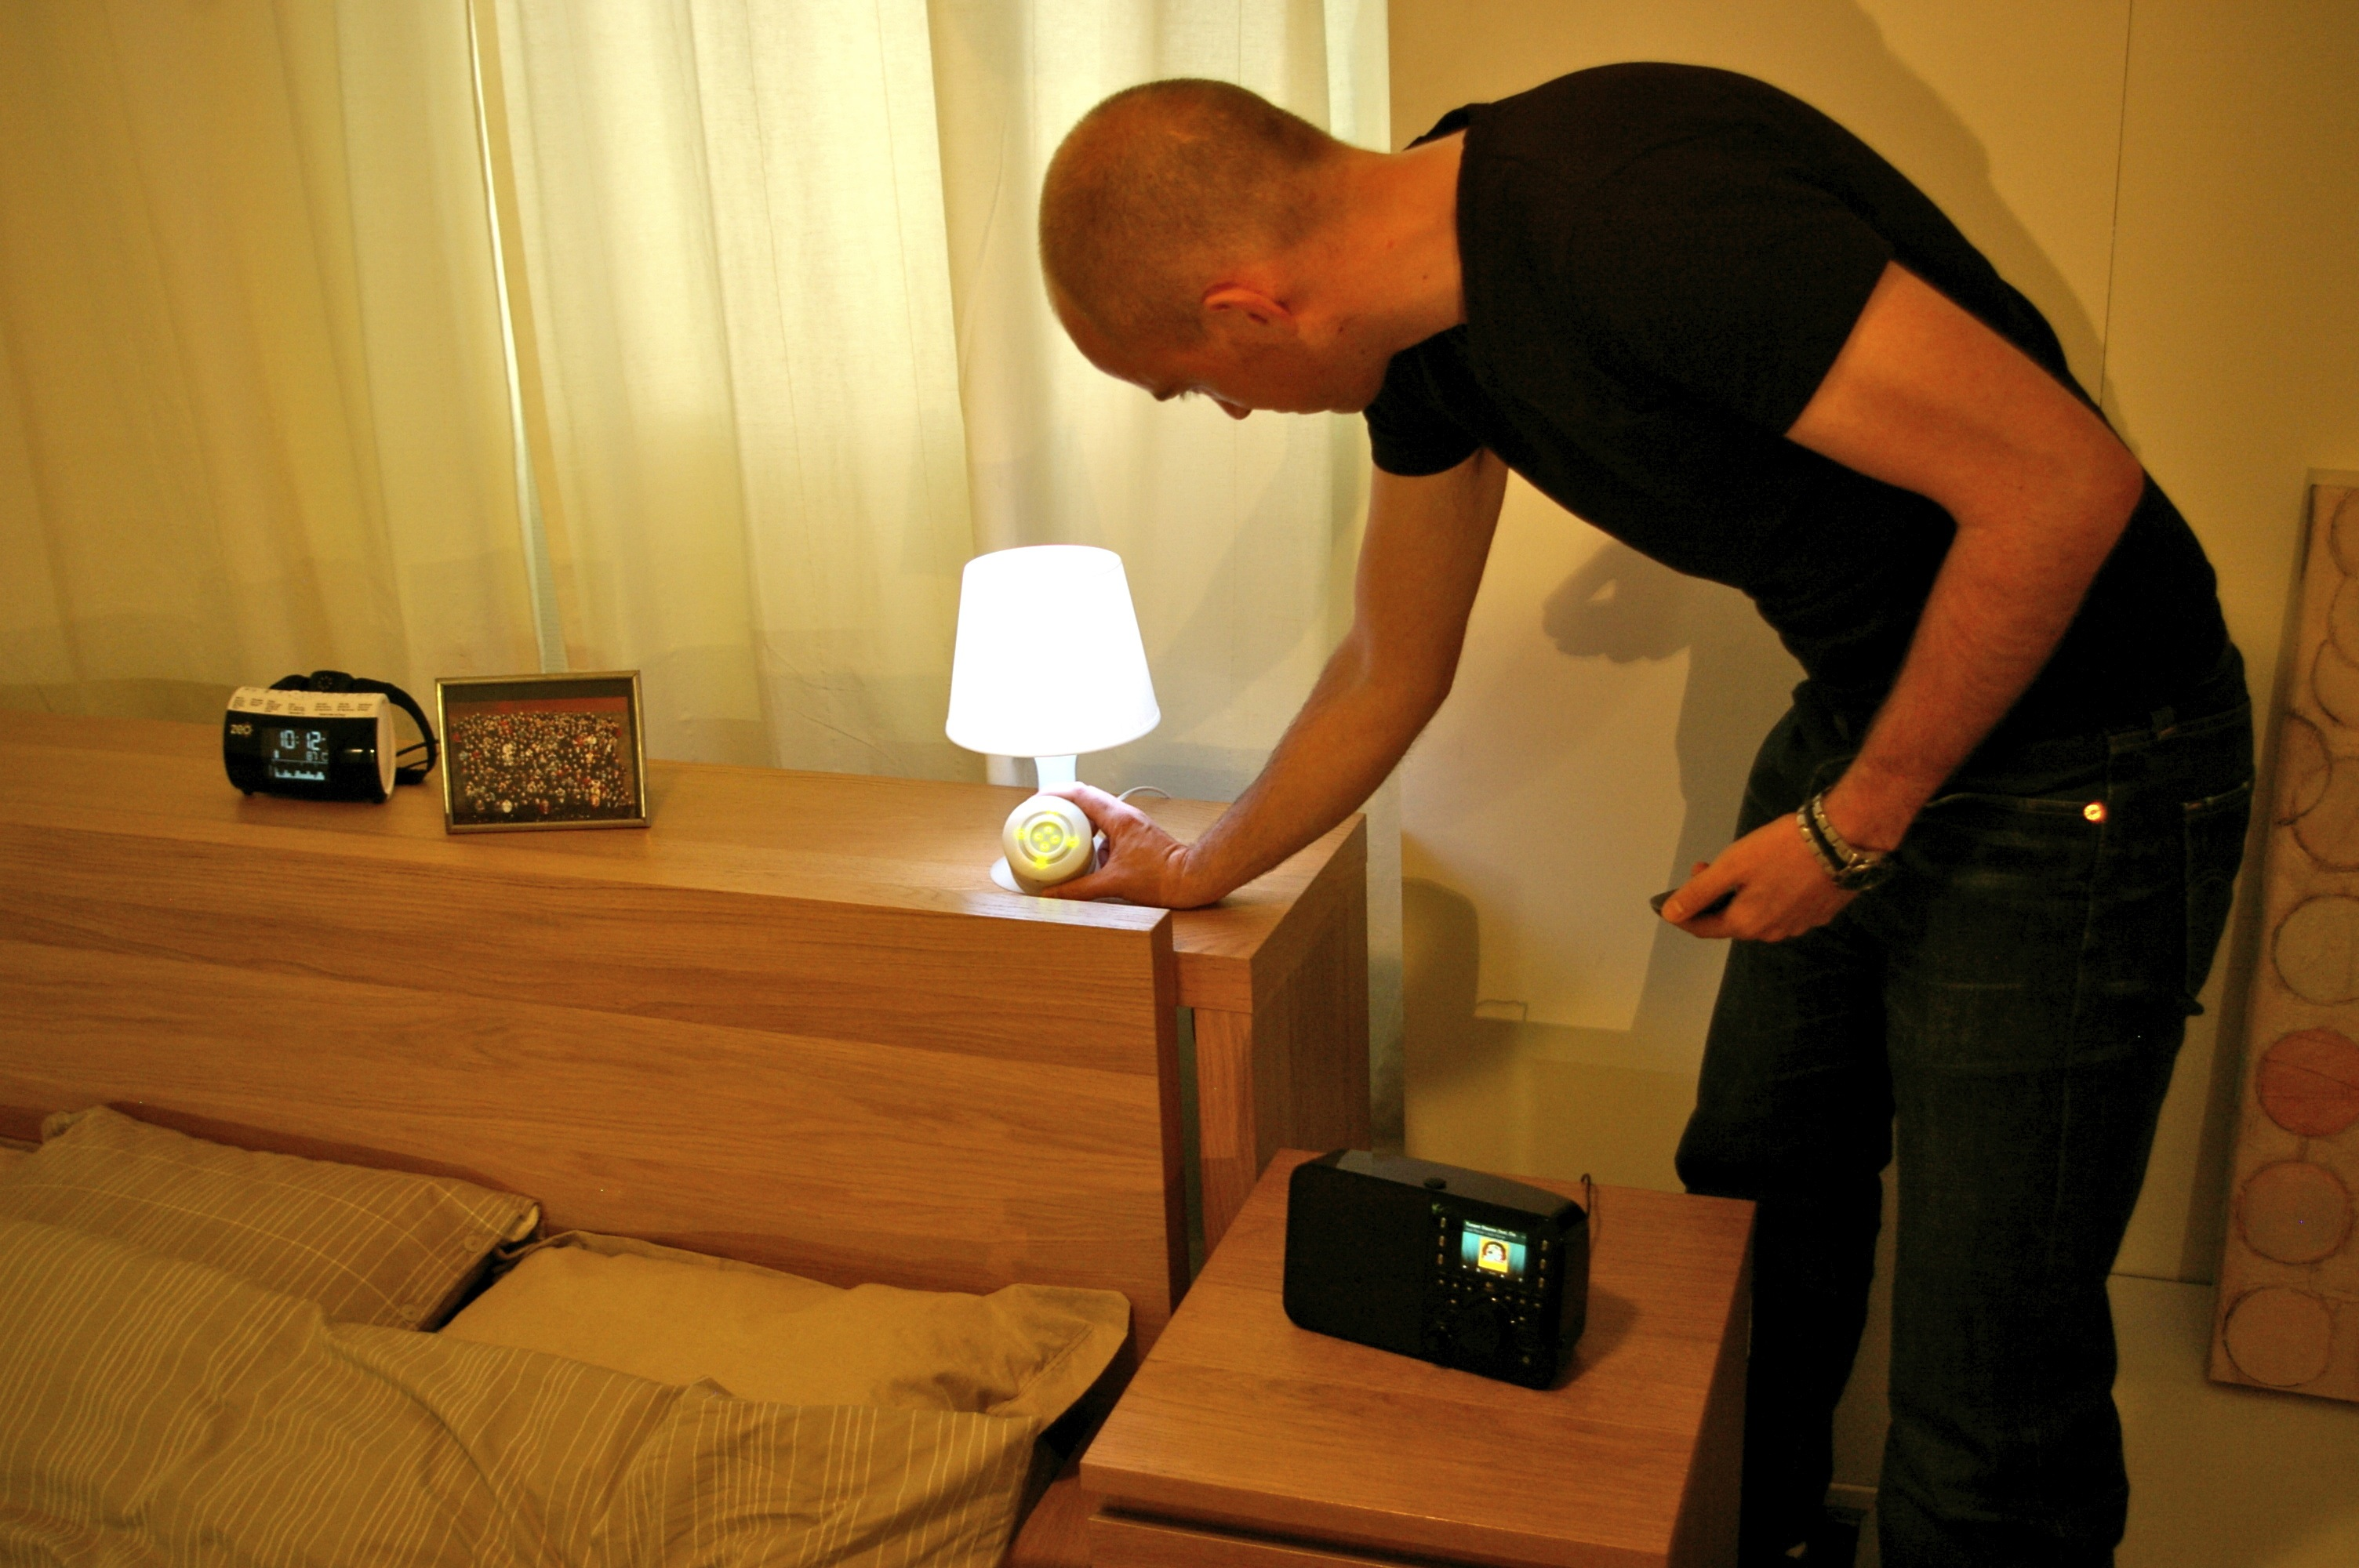
\includegraphics[width=300pt]{sleepscenario}
\caption{The sleep use case scenario, with the Zeo sleep monitor on the left, the dimmable light and the Connector object in the middle, and the Squeezebox on the right}
\label{sleepusecase}
\end{figure}

\subsection{Zeo}

The Zeo sleep monitor is shown on the left-hand side of Figure \ref{sleepusecase}. The Zeo headband, shown in Figure \ref{headband}, uses three silver conductive fabric sensors to collect \ac{EEG} signals while a person is sleeping. The signals are amplified and features are extracted using a \ac{FFT}. An \ac{ANN} is then used to estimate the probability of a person being in a certain phase of sleep\cite{Rubin2009}. The sleep stages are Awake, \ac{REM} Sleep, Light Sleep, Deep Sleep or Undefined. 

\begin{figure}
\centering
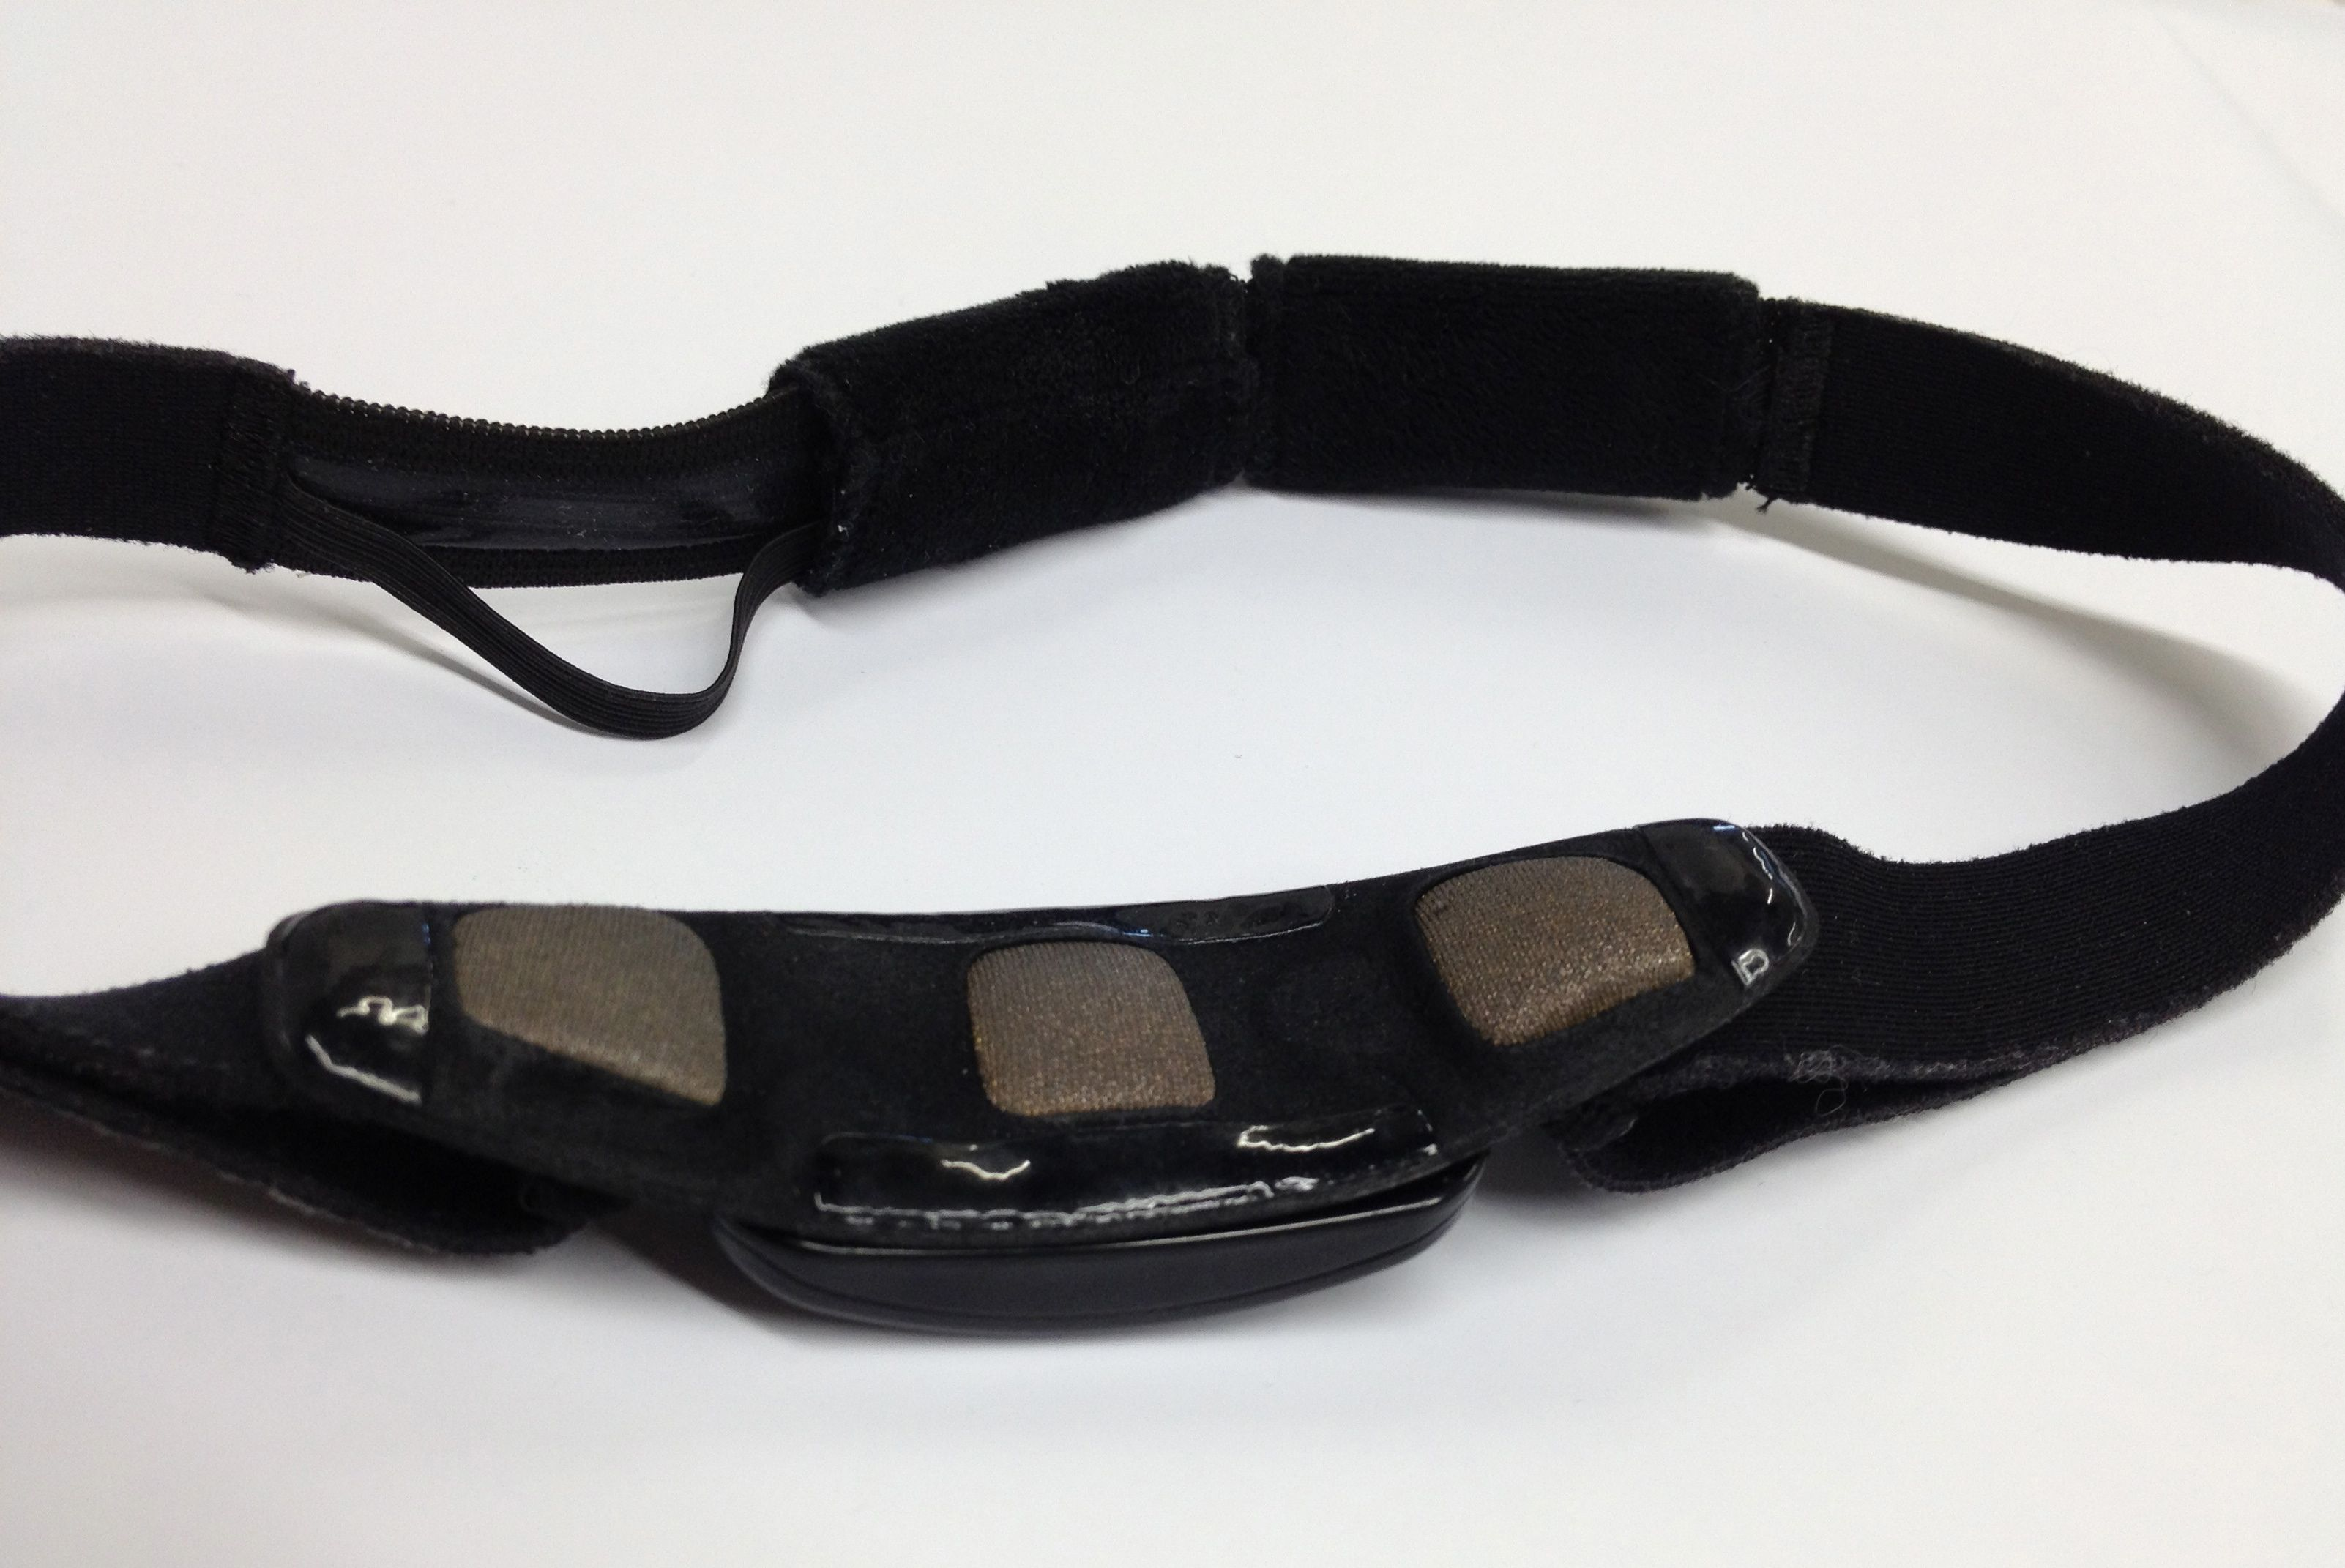
\includegraphics[width=300pt]{headband}
\caption{The Zeo headband}
\label{headband}
\end{figure}


Sleep data is stored on an SD card on the device and can be uploaded to the Zeo MySleep\footnote{http://mysleep.myzeo.com} website. Zeo created the Data Decoder Card library\footnote{http://developers.myzeo.com/data-decoder-library/} that allows developers to decode the sleep data without uploading the data to the MySleep website. We also built a USB cable that connects to a serial port on the back of the device. With this cable you can access the raw data coming from the headband sensor. %-- a diagram indicating how the USB cable should be connected to the Zeo is shown in Figure \ref{zeoBack}.

% \begin{figure}
% \centering
% 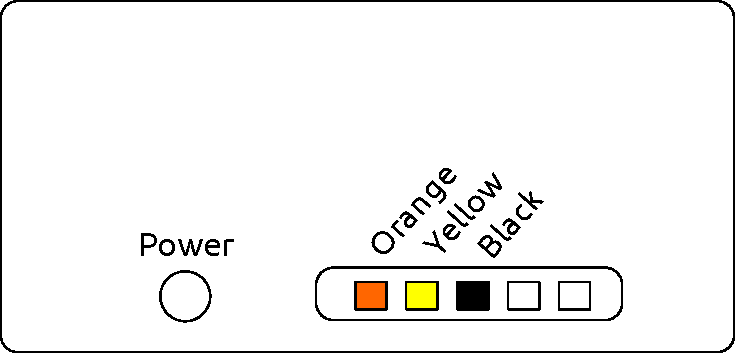
\includegraphics[width=300pt]{ZeoBack}
% \caption{Connecting a USB cable to the debug port of the Zeo sleep monitor}
% \label{zeoBack}
% \end{figure}

When the device is connected via a USB cable, we have real-time access to the generated events. Events that could be interesting to other smart objects in the environment include:

\begin{itemize}
	\item \texttt{NightStart} - time when first ``Awake'' hypnogram occurs
	\item \texttt{SleepOnset}
	\item \texttt{HeadbandDocked} and \texttt{HeadbandUndocked}
	\item \texttt{AlarmOff}, \texttt{AlarmSnooze} and \texttt{AlarmPlay}
	\item \texttt{NightEnd}
	%\item \texttt{NewHeadband}
\end{itemize}

% The Zeo Raw Data Library\footnote{http://sourceforge.net/projects/zeorawdata/} is a Python library to read raw data from the Zeo serial port, using the following commands:
% 
% \begin{minted}{python}
% 	from ZeoRawData.BaseLink import BaseLink
% 	from ZeoRawData.Parser import Parser
% 
% 	# Initialize
% 	link = BaseLink('/dev/ttyUSB0')
% 	parser = Parser()
% 
% 	# Add callback functions
% 	link.addCallback(parser.update)
% 	parser.addEventCallback(eventCallback)
% 	parser.addSliceCallback(sliceCallback)
% 
% 	# Start link
% 	link.start()
% \end{minted}
% 
A \ac{KP} was developed for the Zeo sleep monitor. Although it was not used as part of the final scenario, the Zeo shares its data like sleep states and alarm events in the smart space, which can be used by other devices.
 





\section{Implementation}
\label{D3Implementation}
  
\begin{figure}
\centering
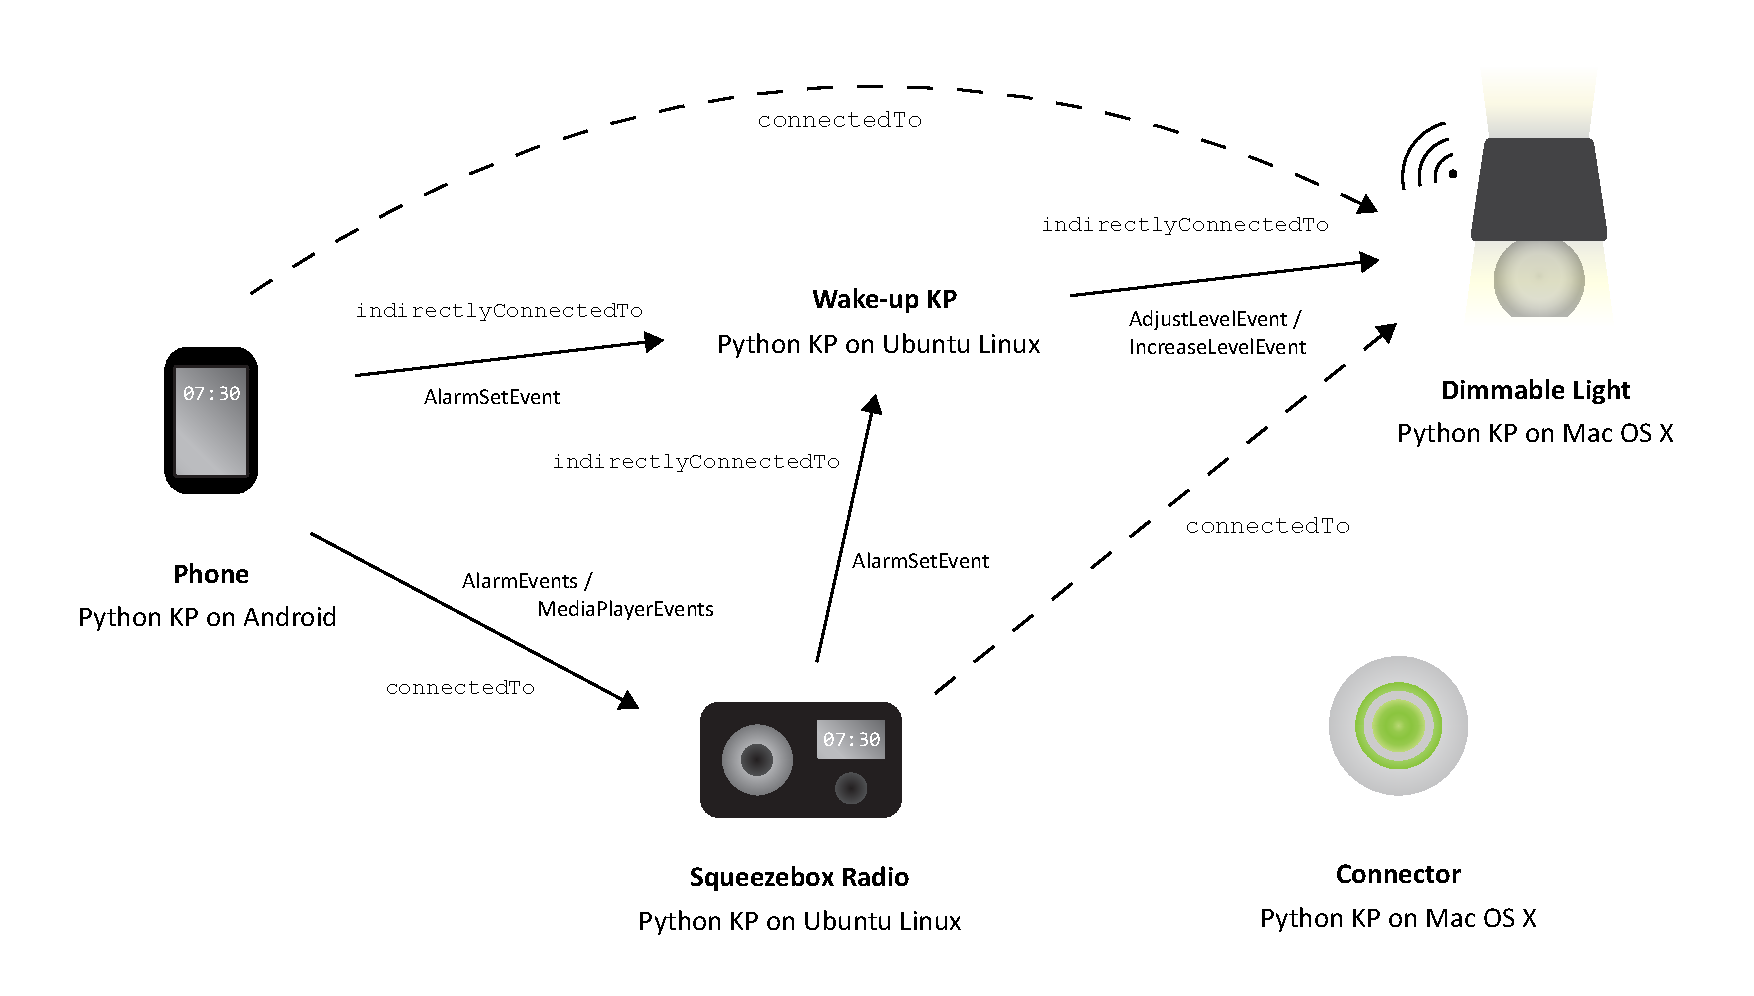
\includegraphics[width=450px]{sleepUseCase}
\caption{An overview of the sleep use case}
\label{sleep}
\end{figure}\marginpar{In the sleep use case we did not make use of the Zeo and its \ac{KP} implementation. It was viewed as a backup device which could be used to introduce additional complexity to the system if necessary.}


%\subsection{Setup} %Method? perhaps a different heading
We started by implementing a very basic configuration, connecting the phone and the internet radio. Based on the capabilities of the devices, possible connections included sharing music player functionality and alarm clock functionality. After implementing the first basic functionalities, we gradually increased complexity by adding another smart object, the dimmable lamp, followed by the implementation of several types of interaction feedback.

% As an interface to semantic connections we used a smart object called the \textit{Connector} (TODO cite). The Connector device follows a tangible interaction approach, enabling users to physically select devices in their environment and directly view and manipulate the connections in a simple, universal way. It is a hand-held device that identifies devices by scanning RFID tags that are located on the devices themselves. By holding the Connector on top of the tag, users can explore the connection possibilities that are visualized with light segments located on top of the Connector. After holding the device in the RFID field for a moment, the device-ID is locked in and the other device to be connected can be selected in a similar fashion. With a push-to-click action a connection between two devices can be established. For removing an existing connection, the ring on the lower part of the device should be pulled until it clicks. Using the Connector and the semantic connections theory allowed us to shift our focus to how subtleties in design and interaction with the smart objects impact the overall user experience. Therefore, the design focus was not on the object interfacing with the connections but rather on the behaviour of the smart objects which are connected.

%\subsection{Implementation Examples}
%\label{section:implementationExamples}



%\subsection{Interaction with semantic connections}
%During the implementation phase, several changes were made to the Connector object to support the functionalities of the sleep use-case. In this section, the most important changes are discussed, as well as the limitations of the Connector's design and their implications for designing for interoperability in general.
%
%\subsubsection{Directionality}
%Although the Connector was originally designed to support the notion of directionality in the interaction with semantic connections, it was not implemented during our previous iteration. The two rings of the Connector's display signify input and output, or source and sink. Where in the previous iteration they indicated the selection of a first and then a second endpoint for the connection (which was symmetric) this was now changed to identify source and sink. The order in which the objects are physically identified is used to determine the direction of the connection. 
%
%Practically this means that the first object a user selects, should be the source object of a connection. When the smart object which is selected is not a source, this is indicated by means of feedback. 
%The same holds for the selection of the second object, which is required to be a sink. When the second object that is selected is not a sink, this is indicated by feedback.
%
%For exploring existing connection, the procedure to follow is similar. The order of selecting define the source and sink to query for an existing connection between the two and feedback is provided accordingly.  
%
%To help users understand why connections are not possible, e.g. their capabilities do not match, the first object is not a source, the second object is not a sink, or an error is returned, the connector should provide distinct feedback for each situation\footnote{The Connector already differentiates between connection possible, connection exists, connection is not possible and a state where both objects are scanned, but an error occurs (e.g. error in the KP, smart object is not subscribed to the SIB). In such cases, both rings remain orange.}. In case the first object is not a source, the outer ring flashed red (indicating it is a sink). When the second object is not a sink, the inner ring flashes red, indicating the object is a source. % explain why this mapping is chosen
%
%% add section on the insights that are gained e.g. limitation of design
%Introducing directionality with the current design of the Connector basically doubles the number of actions as between two given smart objects two connections instead of one may exist. This makes the required actions for more complex configurations cumbersome, and clearly shows the limitations of the current approach. A more comprehensive discussion on directions for a redesign are discussed in section \ref{chapVconnector}.

%\subsubsection{Transitivity}
%With directional connections implemented, the notion of transitivity defines some smart objects as \emph{bridges}. Bridges are different from sources and sinks when they are interacted with, as they behave both as a source and a sink. This becomes particularly clear when exploring existing connections. % add problems surfacing in the interaction.
%
%\subsubsection{Permanent and temporary connections}
%A notion of persistence for a connection was implemented in this iteration. When a source and sink are selected and a connection is possible, temporary connections (in contrast to regular connections; \texttt{connectedTo} relationships) were implemented to enable the use of \emph{preview events} (also see Section \ref{section:augmentedFunctionalFf} below). Temporary connections may also be created between the source and the sink when a possible connection is being explored. Therefore, while the system is in this state, the temporary connection can be used to exchange information. When the connection is confirmed, or when the state is cancelled, the temporary connections either become permanent, or are removed again.

%updates made to the connector

\subsection{Feedback and Feedforward}
\label{section:feedbackAndFeedforward}

In Section \ref{interactionFrogger}, where the Frogger framework of Wensveen \cite{Wensveen2005} was introduced, we also introduced the terminology of augmented and functional feedback/feedforward. We use feedforward to display a device's functional possibilities. We can use feedback to confirm user actions, using augmented feedback where direct functional feedback is not available.\marginpar{In Van der Vlist's thesis \cite{Bram} there is a similar discussion on feedback, that focuses on some of the more user-centred aspects.}

When an alarm is set on the phone, augmented feedback should be given on all devices connected to the phone. For example, consider the setup in Figure \ref{phoneAlarmFeedback}, where the alarm is connected to both the lamp and the Squeezebox radio. 

\begin{figure}
\centering
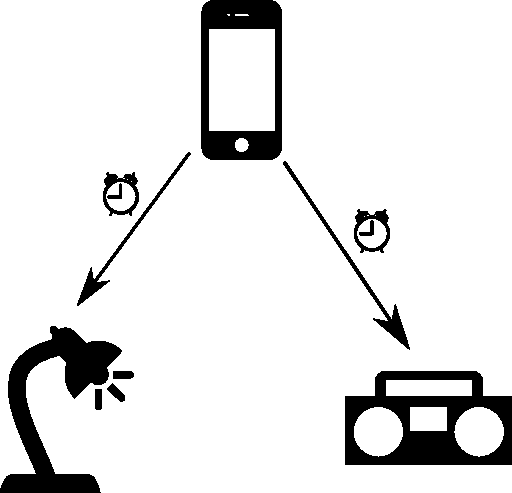
\includegraphics[width=250px]{phoneAlarmFeedback}
\caption{Alarm functionality of the phone shared with the radio and the lamp}
\label{phoneAlarmFeedback}
\end{figure}

Immediate feedback only makes sense when the event and its feedback coincide in time and modality (e.g. audio, visual). When the generated event is a \texttt{SetEvent}, the event itself will occur sometime in the future, so we generate the functional feedforward as augmented feedback instead. For example, for an \texttt{AlarmSetEvent} we generate a $1s$ alert sound on the Squeezebox radio as augmented feedback, providing functional feedforward of what will happen when the alarm is triggered. We also provide visual augmented feedback by displaying a popup message on the display for a few seconds. On the lamp feedback is given in the form of a short light pulse to confirm that it has been notified as well.

Feedback and feedforward need to be carefully designed when smart objects are interconnected. However, as the smart objects themselves are unaware of each other and, at development time, their designers cannot anticipate what other devices users may connect the smart objects to, the total user experience cannot easily be designed. \marginpar{Many solutions for interconnecting devices often employ the \emph{vendor lock-in} strategy, which enables manufacturers to have full control over their ecosystem of products and the resulting user experience.} In this section we will describe how feedback and feedforward were used to enhance the user experience and enable devices that are in-fact unaware of one another, appear to show awareness of each other to their users. 

\subsubsection{Augmented and functional feedforward}
\label{section:augmentedFunctionalFf}
For semantic connections, functional feedback and feedforward can only be considered for the combination of source and sink. The source object has functional feedforward that may communicate its function. Only when both the source and sink object have been identified, is functional feedforward available for the semantic connection. Important to note is, that  functional feedforward is derived from the intersection of functionalities of both the source and the sink. These functionalities could be ambiguous, as both source and sink may be multifunctional. If this is the case, users should make explicit what information or data they want to exchange by selecting the desired mode on the source object (e.g. selecting the alarm application on your smart phone to share the alarm time or go to a picture viewer when pictures should be exchanged), restricting the possibilities. If this is not possible, or a multifunctional smart object is connected when it is in idle mode, semantic reasoning could be used to match all meaningful capabilities of the source and sink objects.

Whenever users wish to make a connection, they have certain expectations. We can employ functional feedforward to influence these expectations. Additionally, we can enhance the user's understanding by explicitly adding augmented feedforward (i.e. augmented \emph{functional} feedforward in contrast to augmented \emph{inherent} feedforward). In the sleep use-case we employed augmented feedforward in the process of exploring connection possibilities i.e. before the connection is made. We do this by giving a \emph{functional preview} on the sink object, viewing the functionality of the connection that is currently explored. Our reasoning is, that only when both source and sink are identified, we can speak of a semantic \emph{connection} and, by giving the feedforward at the sink, we ensure that the sink object is in fact capable of producing this feedforward (i.e. has the necessary capabilities). Additionally the location of the feedforward corresponds to the location where the action (identifying the sink object) was performed. To do so, a \texttt{PreviewEvent} is generated  when a possible connection is being explored, displaying the possible functionalities enabled by the connection.

\begin{example}
\label{phoneToSqueezebox}
When a user, after having identified the phone as a source object, identifies the internet radio as a sink, the display of the internet radio displays a message: ``Alarm can be shared'' and ``Music can be played''. Previews can also be less explicit, like briefly sounding an alarm and playing a short music clip. Note that the preview can be ignored or bypassed by establishing a connection.
\end{example}

\begin{example}
\label{squeezeboxToLamp}
For exploring a connection between the internet radio and the dimmable lamp, the lamp simulates a wakeup sequence, increasing the light level from zero to its maximum intensity in a given period of time (in our implementation three seconds). This may be enhanced with simulating an alarm at the Squeezebox radio when the maximum of the intensity is reached. 
\end{example}

Practically, this means that the designer/developer of a smart object should design the response to  a \texttt{PreviewEvent}. Technically, this is implemented by having the Connector object create a temporary connection to the devices to be connected in order to generate a \texttt{PreviewEvent}. This \texttt{tempConnectedTo} property is a sub-property of the \texttt{connectedTo} property (which denotes a regular semantic connection). This means that the smart objects will handle it as if it is a regular connection, and when the Connector object removes the \texttt{tempConnectedTo} relationship, the inferred \texttt{connectedTo} relationship will disappear as well. The type of functionality the preview is for, is added to the preview event as a data value.

The system behaves differently depending on the type of relation between the smart objects. When there is an indirect connection, i.e. going through a semantic transformer, the preview event is sent to the semantic transformer (Figure \ref{functionalPreview}) instead of the sink object directly (Figure \ref{functionalPreview1}). Additionally, a temporary connection is made between the semantic transformer and the sink, ensuring that the sink displays the correct feedforward when the \texttt{PreviewEvent} is received.

%When the semantic transformer receives the \texttt{PreviewEvent}, it generates yet another event for the preview (as was designed by the developer). %Because of the temporary connection between the source and the sink (going through the Connector), the sink responds to the (preview) event \emph{originating} from the source (Figure \ref{}).

\begin{figure}
\centering
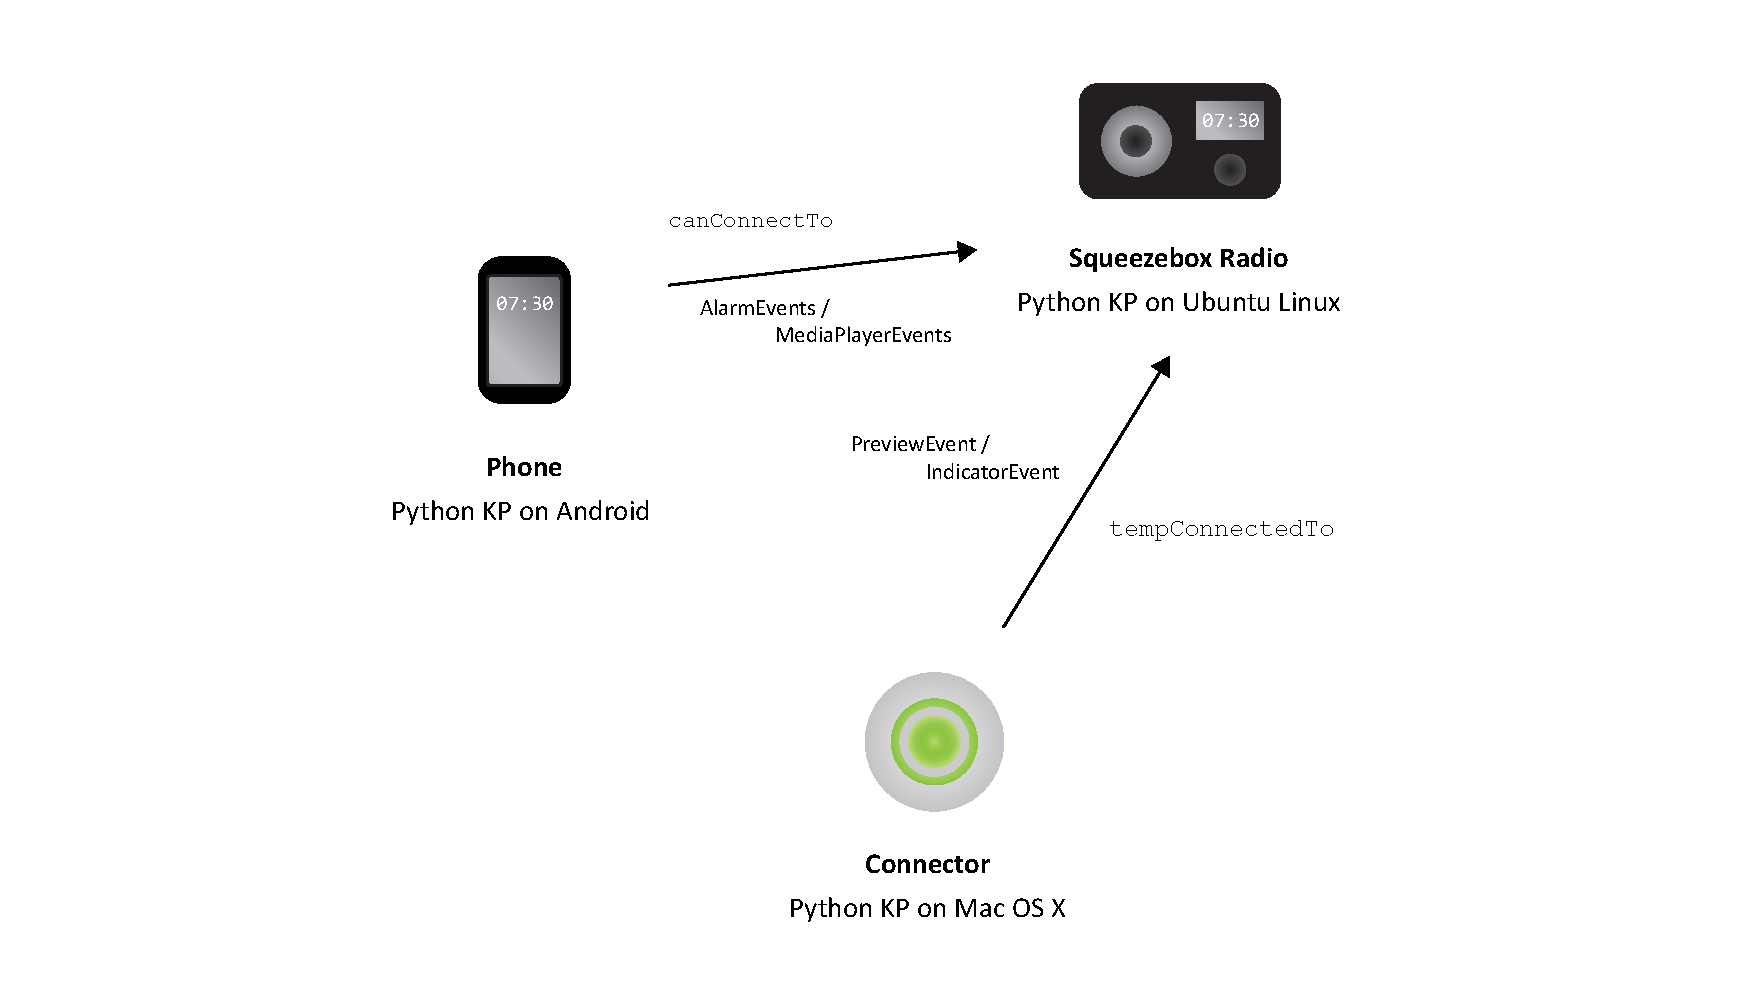
\includegraphics[width=450px]{functionalPreview1}
\caption{Temporary connections for a \texttt{PreviewEvent} when source and sink are directly connected}
\label{functionalPreview1}
\end{figure}

\begin{figure}
\centering
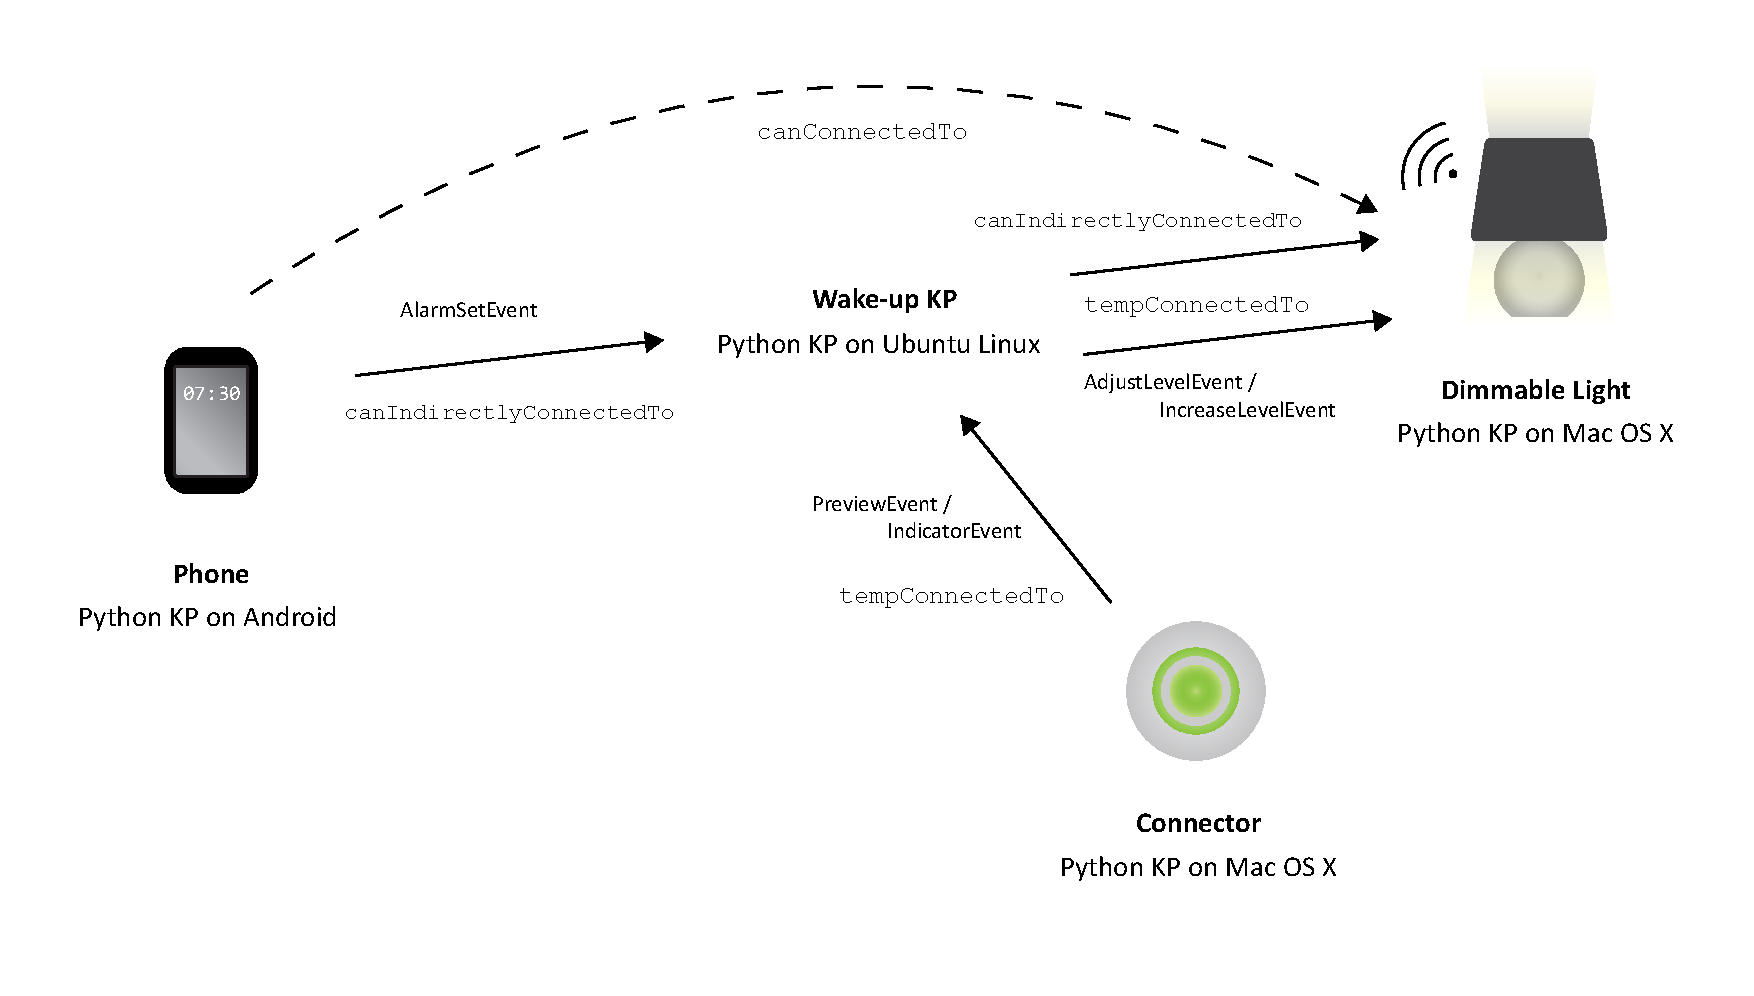
\includegraphics[width=450px]{functionalPreview}
\caption{Temporary connections for a \texttt{PreviewEvent} when source and sink are connected via a semantic transformer}
\label{functionalPreview}
\end{figure}

\subsubsection{Functional feedback}
In many cases functional feedback of a semantic connection is trivial, for example hearing sound from a speaker that was just connected to a media player, or seeing photos on a TV when it is connected to a smart phone. However, functional feedback may only be available at another place or at another time. If we for instance take the example of synchronising a phone's alarm with the alarm radio, the real functional result may be hearing the radio play a song at the alarm time that was set on the phone. 

In such cases, the interaction designers should use augmented feedback as an \emph{indicator} that the alarm time was successfully set. When a semantic connection exists between a source and a sink, actions at the source should also be indicated at the sink. 

If the source and sink objects are in different locations, interaction designers should make sure that feedback is visible for a prolonged time period, or until it is dismissed by the user. This is to ensure that the indicator of the performed action will be noticed by the user. For the same reason, the order of connecting two spatially separated objects together is important, ensuring that establishing the connection happens in proximity of the sink, so that the feedback can be observed. 

\begin{example}
When music is playing on the phone and a connection is made between the phone and the internet radio, functional feedback is immediately given: the internet radio starts playing the same music, and an image of the album cover is displayed. The music on the source (phone) is muted, as the music playing on the internet radio is of a higher fidelity, and both share the same physical space. Context information, such as place/location, can be used to infer the correct behaviour.
\end{example}

\subsubsection{Augmented feedback} 
If there is no immediate link between action and function  (e.g. functional result is delayed, information is given about an internal state change), augmented feedback can be used to provide this information. We use an \texttt{IndicatorEvent} to provide augmented feedback when smart object is connected and there is no immediate functional feedback, e.g. a sink ``beeping'' when the alarm is set on the source.  The type of feedback required depends on the functionality of the connection. It is important for the feedback to coincide in time and modality with the event generated, as to maintain the causal link that is perceived by the user.

When a connections exists and an action performed on the source that has no immediate functional feedback, augmented feedback is provided to serve as an indicator. This feedback is  provided by the smart objects that are connected, in the modality that is supported by their interaction capabilities. Designers should aim for maintaining the modality of the augmented information across the smart objects. Additionally, ensuring that the feedback occurring at distributed objects coincide in time may strengthen the perceived causality of the link. Indicator events may also be used to indicate existing connections, e.g. when a user wishes to see what smart objects are currently connected to a source.  

\begin{example}
When the phone is connected to the internet radio and the internet radio is connected to the dimmable lamp, both the internet radio and the lamp gives augmented feedback when an alarm is set. The internet radio displays the alarm-set screen, confirming the alarm time and the dimmable lamp slowly flashes, to indicate that they are both connected and that the action on the source is confirmed.
\end{example}

%end TiiS



%\subsubsection{The Connector object}
%
%TODO Explain Connector functionality
%
%\begin{figure}[bth]
%\begin{msc}
%msc {
%	//hscale = "1.5";
%	
%    connector [label="Connector Object"], sib [label="SIB"];
%    connector=>connector [label="Scan first smart object"];
%    connector->sib [label="Retrieve name from tag"];
%    sib->connector [label="Name of first smart object"];
%    connector=>connector [label="Scan second smart object"];
%    connector->sib [label="Retrieve name from tag"];
%    sib->connector [label="Name of second smart object"];
%    connector->sib [label="Are they connected?"];
%    sib->connector [label="Not connected"];
%    connector->sib [label="Can they be connected?"];
%    sib->connector [label="Connection possible"];
%}
%\end{msc}
%        \caption{Connecting two devices using the Connector object}
%        \label{connectorSequence}
%\end{figure}



%\section{Evaluation}

% The sleep use case acted as an evaluation of the completeness and applicability of our semantic connections theory, evaluating whether: (a) the defined concepts in our theory are sufficiently defined to use them to implement the required functionalities, (b) the defined concepts can be used universally (for different use cases) and (c) the defined concepts form a complete set to describe the behaviour of semantic connections. Additionally, the implementation served as an example of how our theory can be used in a relevant and contemporary setting. We describe implementation details of how the concepts of the theory are modelled and conclude with changes and additions to the theory that were deemed necessary. 


\section{Discussion \& Conclusion}


% \subsection{Mismatches between device states}
% 
% Interaction events (Chapter \ref{EventModelling}) cause device state changes. When smart objects are interconnected, mismatches in device states may occur, as not all interaction events cause the same state transitions in all smart objects. The design decision to describe the interactions in terms of events as opposed to states was based on the idea that states can be logically inferred from events. Exchanging the events still leaves some autonomy to the smart object (or its developer) to decide what to do with the event. However, only sharing events is not always enough to create consistent behaviour. 
% 
% It is the responsibility of the source to communicate all state changes in the form of events, in order for the sink to keep in sync. Even then, it is still possible for two smart objects to be in different states while connected. Consider the case where the mobile phone is connected to the internet radio, sharing both alarm and music functionality. The user opens the music player on the mobile phone and presses Play, which causes the music to play back on the internet radio. As shown in Figure \ref{fsmPlayAlarm}, an \texttt{AlarmAlertEvent} generated by the mobile phone will cause the internet radio to go into an \texttt{Alarm} state. When the alarm is dismissed on the mobile phone, the internet radio will go into a \texttt{Pause} state, as this is the default behaviour when the alarm is dismissed on the internet radio itself. The mobile phone, however, is now in the \texttt{Play} state. To prevent this state mismatch, the mobile phone should not only send the \texttt{AlarmDismissEvent} that was generated through the user interaction, but also a \texttt{PlayEvent} to indicate that it is now playing music again.
% 
% 
% \begin{figure}[bth]
% %\begin{dot2tex}[dot,options=-tmath --autosize --cache]
% %digraph G {
% 	\digraph[scale=0.5]{MyGraph}{
% 	%rankdir=LR;
% 	font="Ubuntu";
% 	compound=true;	
% 	subgraph cluster0 {
% 	label="Mobile Phone";
% 	alarm1 [label=Alarm];
% 	play1 [label=Play];
% 	pause1 [label=Pause];
% 	pause1 -> play1 [label=Play];
% 	play1 -> alarm1 [label=Alarm];
% 	alarm1 -> play1 [label=Dismiss];
% 	play1 -> pause1 [label=Pause];
% 	}
% 	subgraph cluster1 {
% 	label="Internet Radio";
% 	alarm2 [label=Alarm];
% 	play2 [label=Play];
% 	pause2 [label=Pause];
% 	pause2 -> play2 [label=Play];
% 	play2 -> alarm2 [label=Alarm];
% 	alarm2 -> pause2 [label=Dismiss];
% 	play2 -> pause2 [label=Pause];
% 	}
% 	play1 -> pause2 [ltail=cluster0, label=AlarmDismissEvent];
% 	}
% %\end{dot2tex}
%     \caption{State mismatch between phone and internet radio}
%    \label{fsmPlayAlarm}
% \end{figure}



%We encountered a problem with state mismatches in our sleep use case that resulted in unexpected behaviour. In this specific case, the mobile phone was connected to the internet radio, sharing both alarm and music functionality. If the user opens the music player on the mobile phone and presses Play, it causes the music to play back on the internet radio. Besides playing music, an alarm was also set. When the \texttt{AlarmAlertEvent} generated by the mobile phone occurs, both the phone and the internet radio go to an alarm state. Dismissing the alarm on the phone causes the internet radio to go into a \texttt{Pause} state, as this is the default behaviour when the alarm is dismissed on the internet radio itself. The mobile phone, however, is now in the \texttt{Play} state (although no audio is audible since the speakers of the phone are muted because of the connection to the internet radio). In order to play music again, the phone needs to be paused first, followed by pressing play, to get the device states back into sync. Figure \ref{FSMalarmDismiss} displays this behaviour using a finite state machine.


%To prevent this state mismatch, the mobile phone should not only send the \linebreak \texttt{AlarmDismissEvent} that was generated through the user interaction, but also a \texttt{PlayEvent} to indicate that it is now playing music again.


% \begin{figure}
% \centering
% 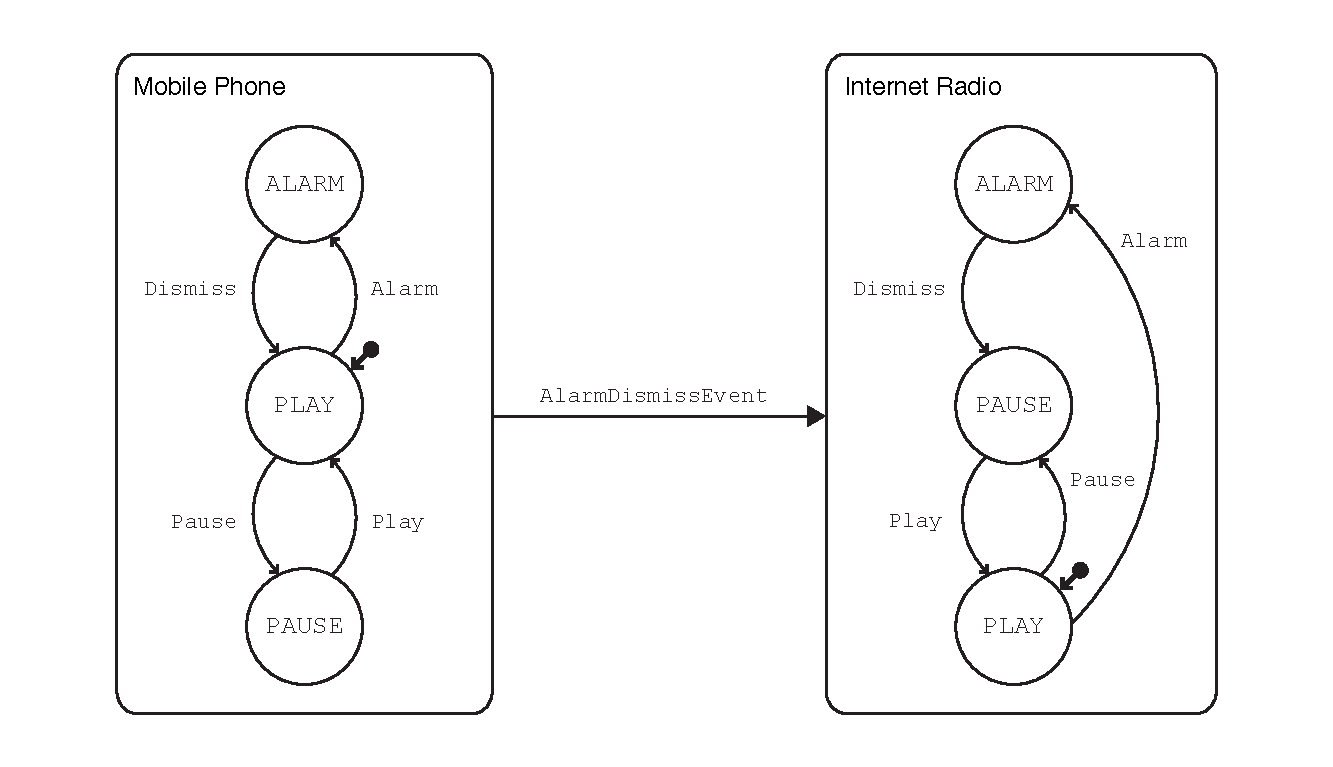
\includegraphics[width=400px]{FSMalarmDismiss}
% \caption{Finite state machine showing the state mismatch between phone and internet radio}
% \label{FSMalarmDismiss}
% \end{figure}


% (removed - Panos)
% \subsection{Setting time on devices}
% 
% For devices to interoperate with one another in a meaningful way, it is imperative that they have the same concept of time and that their clocks are synchronised. For something that should be very trivial, setting the time on devices is surprisingly difficult. Consider the devices we used in our last scenario:
% 
% \begin{itemize}
% 	\item The Zeo sleep manager does not allow for the time to be set remotely - it can only be set manually on the device itself.
% 	\item The Squeezebox radio retrieves the time from the server that it is connected to - you therefore need to be able to set the time on the computer running the server.
% 	\item On Android devices there are documented methods to set the time, e.g. \texttt{setCurrentMillis()}, but due to security restrictions non-system applications are not allowed to access these methods.
% \end{itemize}
% 
% Our workaround was to set the time on the Android phone, which will send the time value with a \texttt{TimeSetEvent}\marginpar{\texttt{TimeSetEvent} is a type of system event. For more information on system events, see Section \ref{SystemEvents}.} to the \texttt{SIB}. When a new \texttt{TimeSetEvent} is received, the Squeezebox KP updates the system time of the Squeezebox Server, requiring super user permissions. The Squeezebox is then restarted to synchronise the local time with that of the server.


%==Causes for increased reasoning time
%One example of where the reasoning time required increased to a number of seconds, was when we made use of the \texttt{owl:sameAs} property.


%\subsection{Conclusion}

The sleep use case acted as an evaluation of the completeness and applicability of the concepts and techniques described thus far. These approaches were distilled into a theory of semantic connections, which forms the basis of the next chapter. The implemented use case evaluated: 
\begin{itemize}
	\item whether the defined concepts and techniques are sufficiently defined to use them to implement the required functionalities;
	\item whether the defined concepts and techniques can be used universally (for different use cases); and
	\item  whether the defined concepts and techniques form a complete set to describe the behaviour of semantic connections.
\end{itemize}

Additionally, the implemented use case can serve as an example of how the theory described in the next chapter is used in a relevant and contemporary setting.

We consider the length of the verbal descriptions in Section \ref{D3Implementation} above to become unwieldy when describing more complex situations. There is a clear need for some kind of diagram notation to describe these situations. In the next chapter we introduce a theory of semantic connections that was created to help solve this problem. We first describe the concepts that are central to this theory, and then introduce a diagram notation based on \acp{FSM}, that can be used to model and explain the different concepts and situations.



\chapter{Semantic Connections Theory}
\label{SemanticConnectionsTheory}

\begin{flushright}{\slshape    
Essentially, all models are wrong, but some are useful.} \\ \medskip
    --- George Box
\end{flushright}



%begin TiiS

Extracting from the lessons learned during the three design iterations, a theory was developed for interacting with a system of devices in a ubiquitous computing environment. This chapter introduces a theory of semantic connections, in which the connections and associations between devices play a central role. Semantic connections focus on the semantics---or meaning---of the connections between entities in a smart environment. 

The theory may be used to analyse (i.e. understand, explain and predict) what happens with interaction events and other interaction data when devices are interconnected and form an ecology of smart objects. As an introduction to the Semantic Connections theory, we first focus on the Semantic Connections user interaction model.

\section{User interaction model}
\label{InteractionModel}

A user interaction model for semantic connections is shown in Figure \ref{model}. It describes the various concepts that are involved in the interaction in a smart environment and shows how these concepts work together. The interaction model was inspired by the \ac{MCRpd} by Ullmer and Ishii \cite{Ullmer2000} which in turn was based on the \ac{MVC} model, both of which are described in Section \ref{mcrpd}. 

\begin{figure}
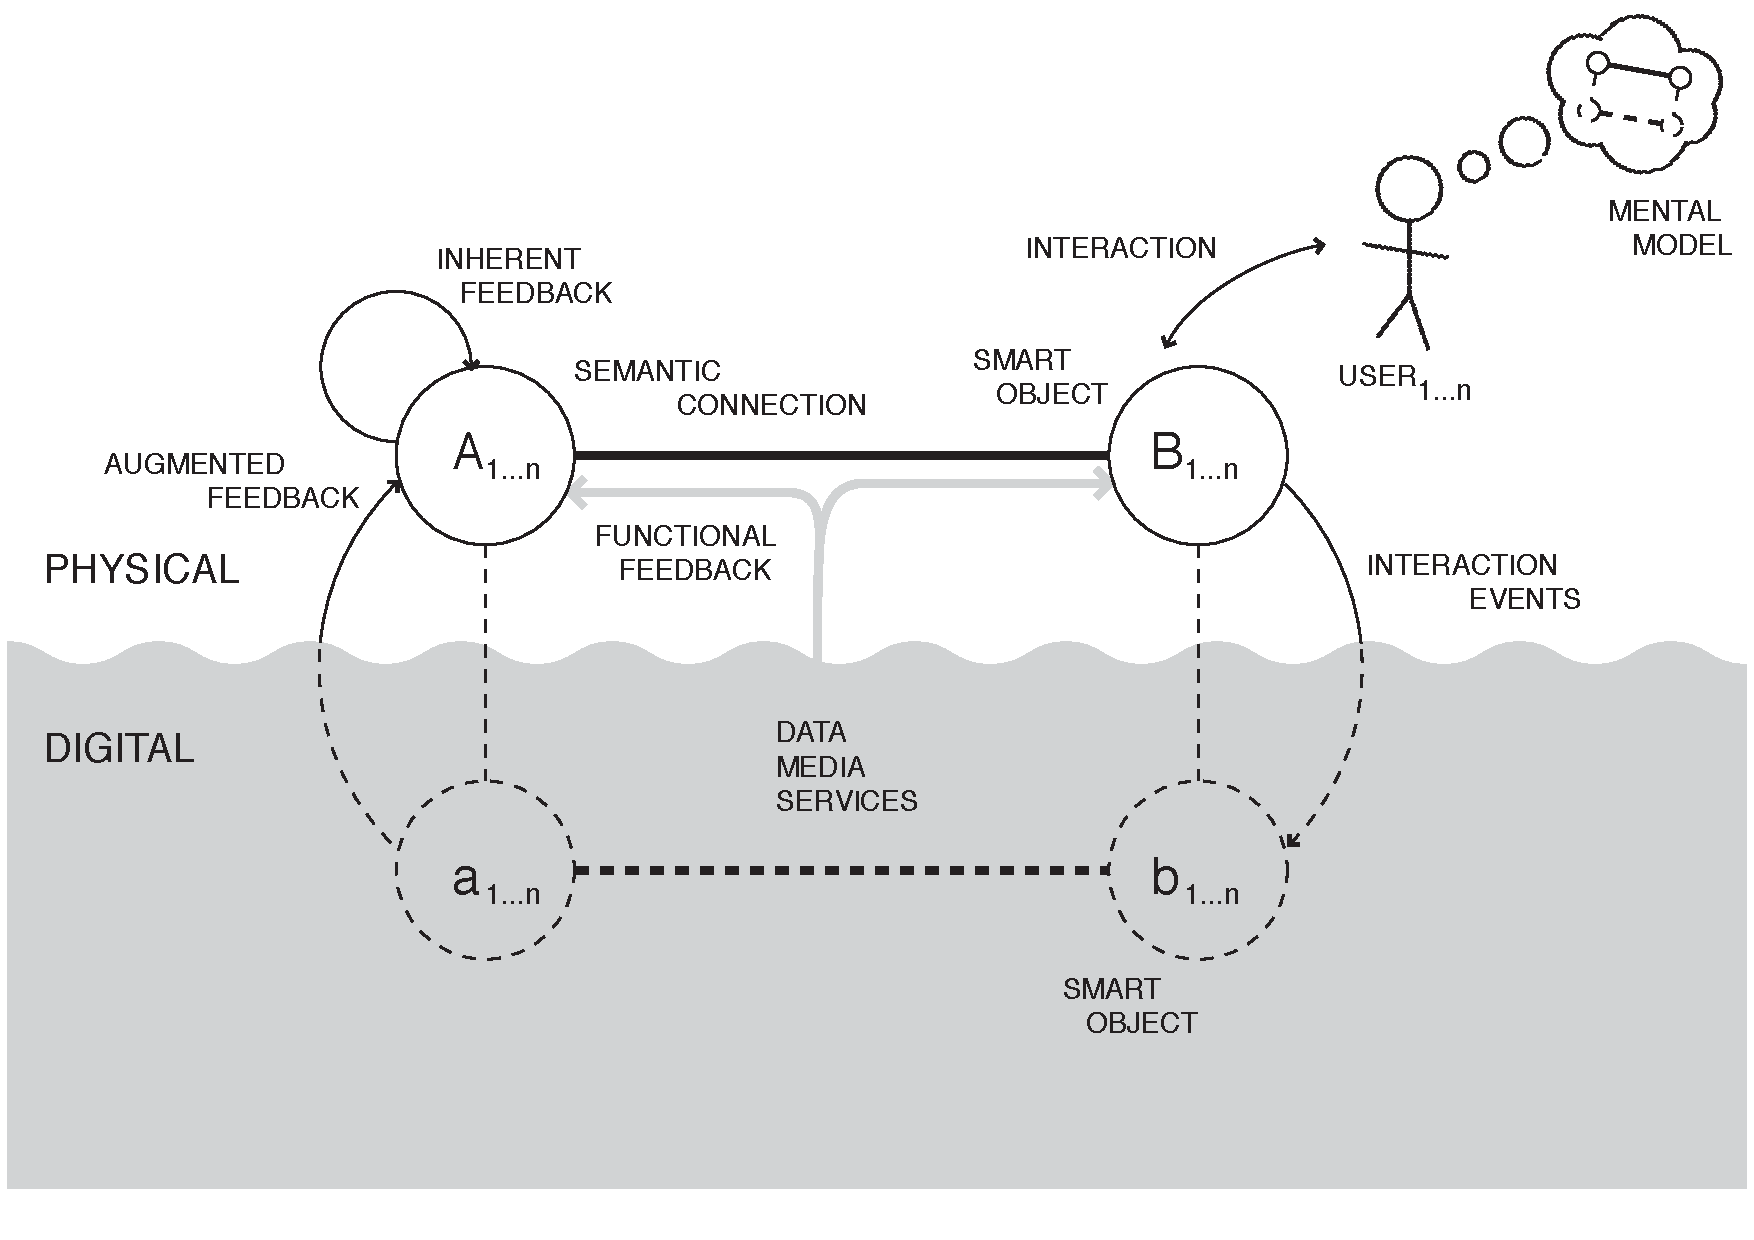
\includegraphics[width=\columnwidth]{InteractionModel}
\caption{Semantic connections user interaction model}
\label{model}
\end{figure}

We first distinguish between the physical and digital domains of the user interaction. A user does not observe directly what is happening in the digital domain, but experiences the effect it has in the physical world by interacting with various smart objects. Semantic connections exist between these objects. By interacting with the objects, users create a mental model of the system that they are interacting with, which only partly includes the digital domain. The digital part manifests itself in the physical world as data, media and services. 

\marginpar{The terminology of inherent, augmented and functional feedforward and feedback is adopted from \cite{Wensveen2004} and was previously introduced in Section \ref{interactionFrogger}.} 
When a user interacts with a smart object, he/she senses feedback and feedforward, directly from and inherent to the controls of the device (inherent feedback), digital information augmented onto the physical world (augmented feedback) and perceives the functional effect of the interactions (functional feedback). The user actions in the physical world are transformed into interaction events and device state changes. This interaction data in terms of user intentions is stored in the smart space. The notion of a smart space means that data are stored either by an information broker or the smart objects themselves, and can be accessed by the other smart objects in the smart space. We use the term smart environment as a broader term to refer to both the digital and physical spaces, which include both the smart space and the smart objects.

\marginpar{Note that in Figure \ref{model} the arrow on the left shows the feedback (or output) of the smart object, and on the right it shows the input (the interaction event). This to avoid repetition, as they may and in most cases will, occur on both sides.}% possibly together with user preferences, defaults and context information.






% In figure (TODO fig vertical view) we describe how user actions with smart objects on the physical lever are translated into interaction events in the digital domain. As user actions are transformed into events, we use the (Nielsen's model) to describe the level along the continuum. 
% 
% To enable user interaction in smart spaces on the level that was sketched in the introduction, the developer community needs to agree on a way of describing the various elements involved in the interactions. These interaction elements or controls are physical by nature (i.e. they are material parts or at least directly perceivable in the physical world), which means that their physical meaning and some of physical properties need to be preserved while describing them. In the sections that follow sections we propose the concepts of interaction primitives (Section \ref{InteractionPrimitives}) and interaction events (Section \ref{InteractionEvents}) as ways to describe these elements and their interactions.
% 
% \begin{figure*}[hbt]
% \centering
% 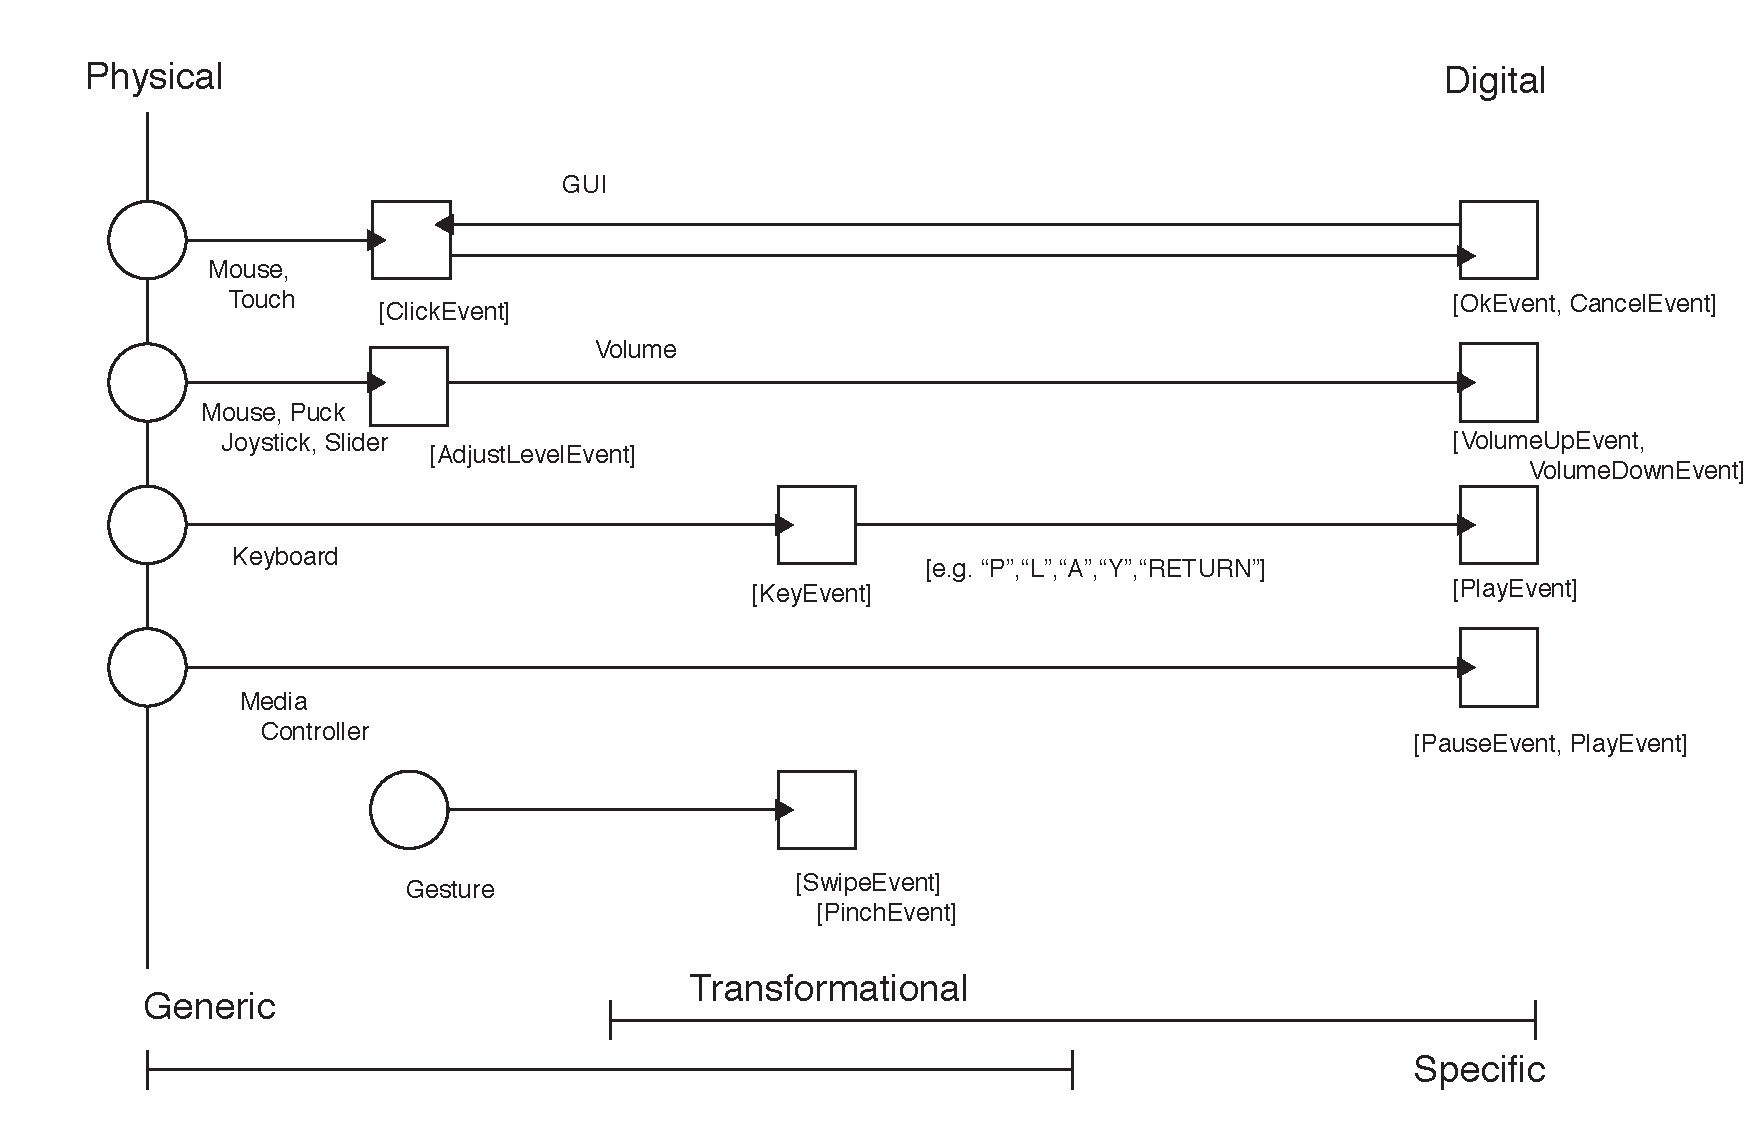
\includegraphics[width=400px]{UserInterfaceModel}
% \caption{User Interface Model}
% \label{interfaceModel}
% \end{figure*} 
% 
% Figure \ref{interfaceModel} shows our proposal to model user interfaces in terms of their physical, real-world interaction properties (like position, movement, rotation, force and torque) and their transformation towards the consequences they have in the digital domain (e.g. triggering interaction events, changing states). The entities represented in the model as circles are what we call \emph{interaction primitives}, the smallest addressable interaction element that has a meaningful relation to the interaction itself. 
%
%On the left-hand side of the figure we plot entities that sense \emph{physical} properties like position, movement or pressure. We consider these properties to be very \emph{generic}, as they do not report a user's intention directly. The inputs first need to be transformed into an intentional event (events that express user intention). This can happen directly, for example pressing a play button, which is transformed into an \texttt{PlayEvent}. It can also follow a series of intermediate transformational steps, where a sequence of interaction events (possibly happening on different devices) may be used to capture the user's intent. This sequence of events is then transformed into a single intentional event.
%
%On the right-hand side of the figure we have the \emph{digital} entities that represent the intentional events. We consider these entities to be very \emph{specific}, as they communicate the (assumed) intention of the user's actions directly.
%
%Entities and their relationships in an interaction together form an \emph{interaction path}. The interaction exchange or action between elements in the path is conducted via one or more \emph{interaction channels} along which information or action is communicated \cite{dubois_2008}. As an example, a typical interaction path in Figure \ref{interfaceModel} would be: 
%
%\begin{quote}\noindent 
%\texttt{Keyboard}  $\rightarrow$ \texttt{KeyEvent} $\rightarrow$ \texttt{PlayEvent} 
%\end{quote}
%
%while an interaction channel exists between \texttt{Keyboard}  and \texttt{KeyEvent}. 
%
%During the transformation from physical to digital, the interaction devices (or their interaction primitives) also move from generic to more specific, where generic user interfaces start off very generic and stay generic or transformational (meaning they have been transformed but still need further transformation). This means that such interaction devices or interaction primitives can still be transformed into many different events or states. When an interaction primitive travels from generic to specific with a single transformation (like the media controller buttons) it means that that these interaction primitives are very specific UI elements (i.e. have one single function). An example of such an interaction primitive would be a hardware button with a specific label that is only used for one function. As another example, consider a gesture; i.e., a (less) generic interaction primitive that transforms from a physical movement that is sensed in a certain way, to the digital representation of that gesture, being a ``pinch'', ``swipe'' etc. The pinch and swipe are still considered transformational because they still need to be transformed further to result in a certain interaction event. However, in the initial transformation, some meaning is preserved (i.e. the physical characteristics of the gesture). These characteristics limit the number of actual events the gesture can still be transformed into, e.g. a ``swipe right'' gesture should not be transformed into a ``navigate forward'' action, as this is the way we usually navigate backwards. Table \ref{transformationTable} shows some of the possible transformational events we consider to be applicable to smart home environments in which multimedia and lighting devices are connected for certain applications.
%
%\begin{table}
%\centering
%\begin{tabular}{|l|l|}
%\hline
%Event & Entity this event can be performed on\\
%\hline
%AdjustLevel & Volume, Lighting \\
%switchOnOff & Lighting, any SmartObject \\
%Navigate & Playlist, Menu, SequentialData \\
%Undo/Redo & Any interaction event \\
%Stop/Start & Application, Media \\
%DragAndDrop & Media \\
%Query & Media, other events \\
%\hline
%\end{tabular}
%\caption{Examples of transformational events in a smart environment}
%\label{transformationTable}
%\end{table} 
%
%Although describing user interaction capabilities of devices according to the user interface model is valid for user interaction in general, it is specifically relevant when we consider the notion of a smart space through which this interaction data can be exchanged. To achieve this, all events that need to be shared must be modelled in a mutually understandable way. A good way of modelling them would be an ontology, as is shown in section \ref{semanticInteraction}. 
%




\section{Smart Objects}

Smart objects are the devices that are connected to the smart space, enabling them to share information with one another. We now define a smart object as follows:

\begin{description}
	\item[Smart Object]A smart object is a device with both computational and network communication capabilities that can be uniquely identified in both physical and digital space.
\end{description}

According to our definition, an \ac{NFC} enabled smart phone is a smart object. A WiFi-connected lamp is also a smart object, given that it can be physically identified, for example by proximity based on signal strength or \ac{RFID}. \marginpar{Note that our definition does not define where the \ac{KP} is situated. For simple smart objects, such as a smart light bulb, the actual \ac{KP} that is communicating to the information broker may be a virtual entity running on any device in the network.}

In terms of our definition, a light switch with an \ac{RFID} tag is not a smart object. A software agent running on a \ac{GUI} (e.g. Microsoft Office's Clippy\footnote{http://en.wikipedia.org/wiki/Office\_Assistant}), is not considered a smart object, even though it is visually perceivable. Despite its apparent physical existence, i.e. physically and digitally identifiable, it is mediated by a computer. In such cases the computer is considered the smart object and not the agent running on it, as the agent is not primarily a physical entity. In the following subsections we describe the concepts specific to the smart objects themselves.

\subsection{Identification}
\label{Identification}
For semantic connections to work in the way they are envisioned in this thesis, a smart object needs to be uniquely identifiable in both the physical and the digital domain. In the physical space it needs to be both user-identifiable and machine-identifiable. A device that is tagged with an \ac{RFID} tag is machine-identifiable in the physical space, and the unique identifier read from this tag is also linked to the digital representation of the smart object. \ac{NFC}---using a near field channel like \ac{RFID} or infrared communication---is an interesting case, because it allows for direct manipulation of wireless network connections by means of proximal interactions \cite{Rekimoto2003}.

Of course, there are many ways in which a smart object may be identified. An IP address makes a device easily identifiable in the digital space, but it is difficult to create a physical representation of this identity. Consider the case where IP addresses are printed on stickers and stuck on computers to make them easier identifiable to IT service personnel. One solution to making these stickers machine-identifiable again is to use \ac{QR} codes, two-dimensional barcodes which can be identified by mobile phone cameras.

\subsection{Interaction primitives}
\label{InteractionPrimitives}

We defined interaction primitives as a way to describe the user interaction capabilities of smart objects in ubiquitous computing environments. \marginpar{Interaction primitives were introduced in Section \ref{sectionSemanticInteractionOntology}.} These interaction primitives are based on the work of Foley, Card and others introduced in Section \ref{interactionTasks}.

The key on a keyboard labelled ``A'' is an interaction primitive, as pressing it not just changes the key's \texttt{Up} state into a \texttt{Down} state, but carries the meaning to \emph{produce} a character ``A''. A gesture \texttt{SwipeLeft} on a touchpad is also an interaction primitive, as this is the smallest addressable element to still have meaning. Describing the input on a lower level would cause it to lose its meaningful relation to the interaction. A touchpad itself is not an interaction primitive but rather an input device. An interaction with the touchpad, annotated with its meaning, can be an interaction primitive. A \ac{GUI} is not an interaction primitive, but a \ac{GUI} element can be.

Interaction primitives are described in terms of their physical properties that are meaningful to a user. For example, an unlabelled button should not only be represented in terms of its \texttt{On} and \texttt{Off} states, but also whether it is in a \texttt{Up} or \texttt{Down} state. This enables the mapping of physical, generic interaction primitives like a rocker switch to specific high-level events like \texttt{VolumeUpEvent}.

An interaction primitive also has a range measure that describes the range of possible values that it can take on. This makes it easier to determine if and how they can be mapped to specific interaction events.

Interaction primitives and interaction events together form an \emph{interaction path} \cite{Dubois2008}. As an example, a typical interaction path would be:
\label{interactionPath}

\begin{quote}\noindent
\texttt{VolumeSliderLeft} $\rightarrow$ \texttt{SlideLeftEvent} $\rightarrow$ \texttt{VolumeDownEvent}
\end{quote}

where the \texttt{VolumeSliderLeft} is an interaction primitive mapped to the \texttt{SlideLeftEvent} interaction event. Based on the available context information, this can in turn be mapped to a more specific \texttt{Volume\-Down\-Event}.


% --- The following could be included for more information on interaction primitives (but remember, TODO parts of this chapter africon)

% \begin{figure*}[hbt]
% \centering
% 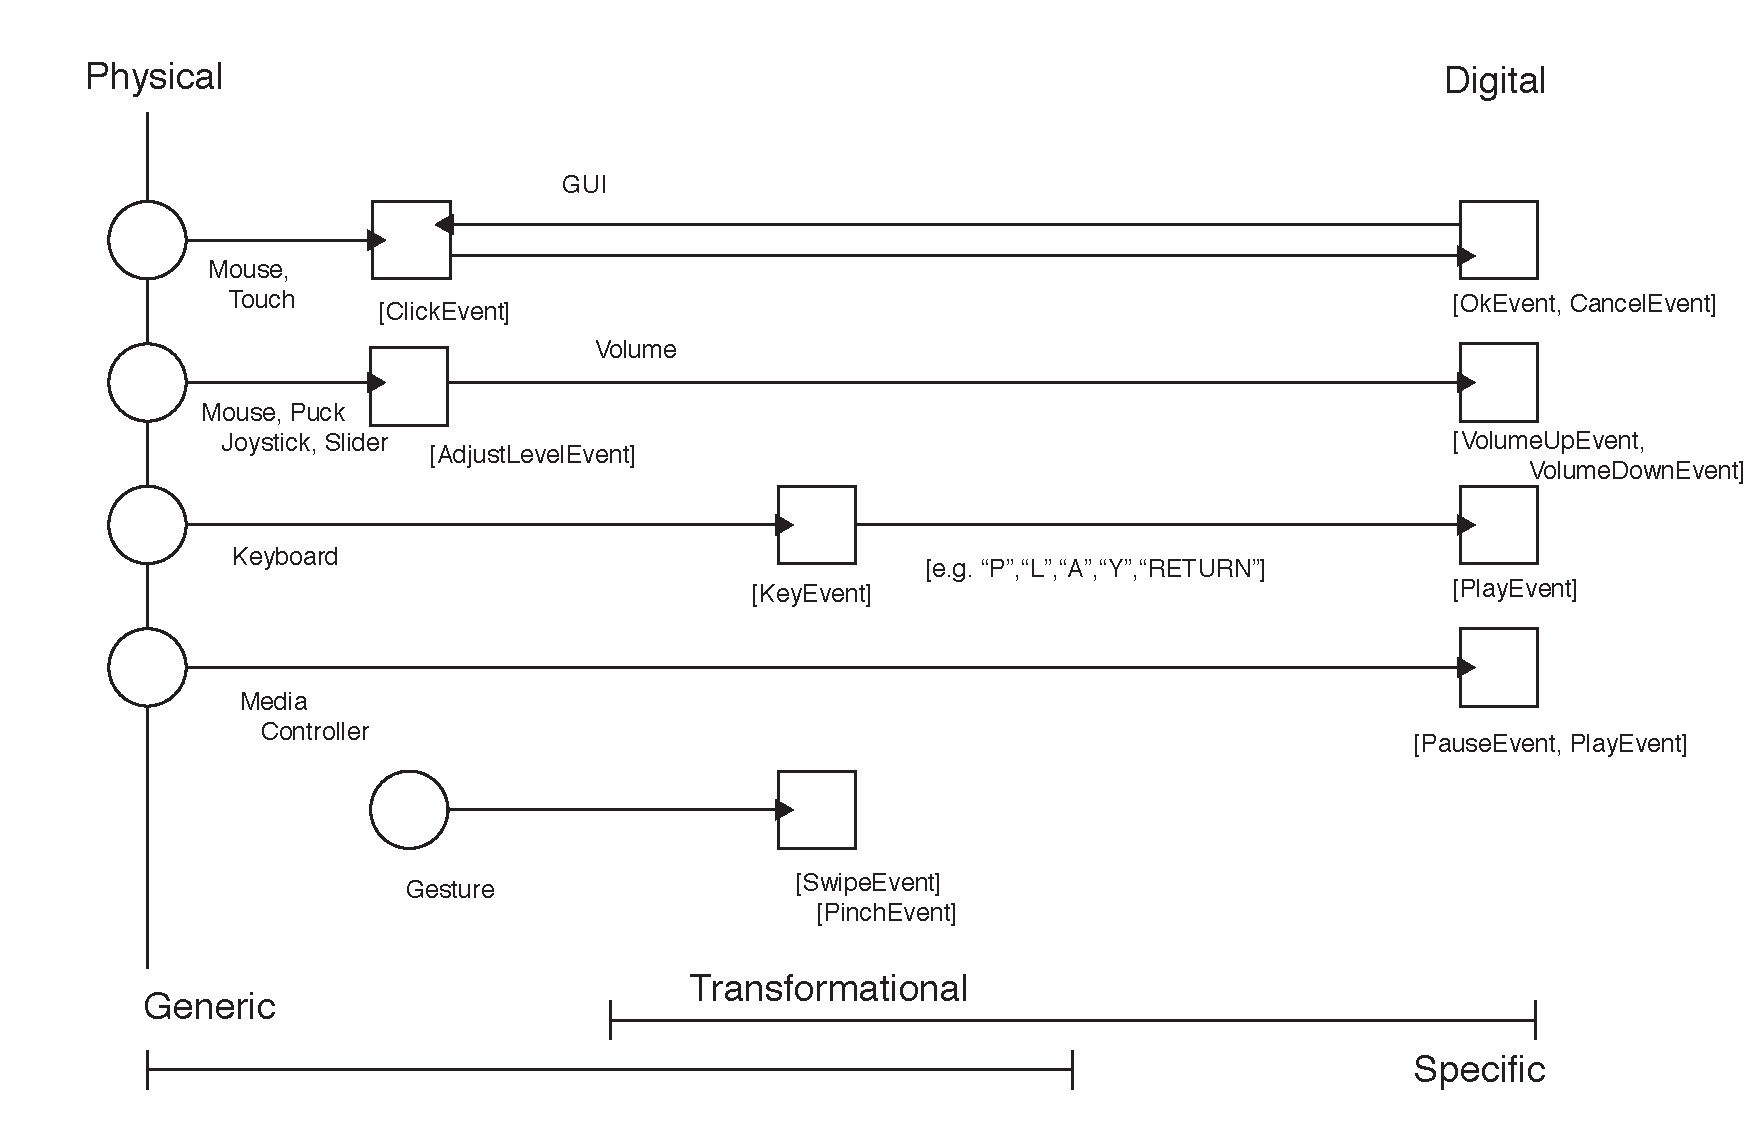
\includegraphics[width=400px]{UserInterfaceModel}
% \caption{User Interface Model}
% \label{interfaceModel}
% \end{figure*} 
% 
% Figure \ref{interfaceModel} shows our proposal to model user interfaces in terms of their physical, real-world interaction properties (like position, movement, rotation, force and torque) and their transformation towards the consequences they have in the digital domain (e.g. triggering interaction events, changing states). Interaction primitives are modelled as circles in this diagram.
% 
% On the left-hand side of the figure we plot entities that sense \emph{physical} properties like position, movement or pressure. We consider these properties to be very \emph{generic}, as they do not report a user's intention directly. The inputs first need to be transformed into an intentional event (events that express user intention). This can happen directly, for example pressing a play button, which is transformed into an \texttt{PlayEvent}. It can also follow a series of intermediate transformational steps, where a sequence of interaction events (possibly happening on different devices) may be used to capture the user's intent. This sequence of events is then transformed into a single intentional event.
% 
% On the right-hand side of the figure we have the \emph{digital} entities that represent the intentional events. We consider these entities to be very \emph{specific}, as they communicate the assumed intention of the user's actions directly.
% 
% Entities and their relationships in an interaction together form an \emph{interaction path}. The interaction exchange or action between elements in the path is conducted via one or more \emph{interaction channels} along which information or action is communicated \cite{Dubois2008}. As an example, a typical interaction path in Figure \ref{interfaceModel} would be:\\
% 
% \noindent 
% \texttt{Keyboard}  $\rightarrow$ \texttt{KeyEvent} $\rightarrow$ \texttt{PlayEvent}\\ 
% 
% 
% while an interaction channel exists between \texttt{Keyboard}  and \texttt{KeyEvent}. 
% 
% During the transformation from physical to digital, the interaction devices (or their interaction primitives) also move from generic to more specific, where generic user interfaces start off very generic and stay generic or transformational (meaning they have been transformed but still need further transformation). This means that such interaction devices or interaction primitives can still be transformed into many different events or states. When an interaction primitive travels from generic to specific with a single transformation (like the media controller buttons) it means that that these interaction primitives are very specific UI elements (i.e. have one single function). An example of such an interaction primitive would be a hardware button with a specific label that is only used for one function. As another example, consider a gesture; i.e., a (less) generic interaction primitive that transforms from a physical movement that is sensed in a certain way, to the digital representation of that gesture, being a ``pinch'', ``swipe'' etc. The pinch and swipe are still considered transformational because they still need to be transformed further to result in a certain interaction event. However, in the initial transformation, some meaning is preserved (i.e. the physical characteristics of the gesture). These characteristics limit the number of actual events the gesture can still be transformed into, e.g. a ``swipe right'' gesture should not be transformed into a ``navigate forward'' action, as this is the way we usually navigate backwards. 

% ---- end


%Table \ref{transformationTable} shows some of the possible transformations we consider to be applicable to smart home environments in which multimedia and lighting devices are connected for certain applications.

% \begin{table}
% \centering
% \begin{tabular}{|l|l|}
% \hline
% Event & Entity this event can be performed on\\
% \hline
% AdjustLevel & Volume, Lighting \\
% switchOnOff & Lighting, any SmartObject \\
% Navigate & Playlist, Menu, SequentialData \\
% Undo/Redo & Any interaction event \\
% Stop/Start & Application, Media \\
% DragAndDrop & Media \\
% Query & Media, other events \\
% \hline
% \end{tabular}
% \caption{Examples of transformational events in a smart environment}
% \label{transformationTable}
% \end{table} 

%Although describing user interaction capabilities of devices according to the user interface model is valid in general, it is specifically relevant when we consider the notion of a smart space through which this interaction data can be exchanged. To achieve this, all events that need to be shared must be modelled in a mutually understandable way. 

%When modelling, only that which is meaningful to be shared with other devices is considered. It is not necessary to describe interactions that are internal to the device and that are not shared.. An accelerometer for example may be modelled as a separate device, sharing the raw accelerometer data to be used by other devices. However, when integrated into smart phones, the accelerometer's data can often be abstracted as part of an interaction path, e.g. to only share the orientation of the device or specific gestures measured with the accelerometer. The raw values may, in this case, need only to be available to the device to be used by the developers of other applications.





% \label{paths}
% \emph{Media paths} connect devices based on their media capabilities, allowing content to be streamed from one device to another. A semantic reasoner is used to perform media type matching, e.g. to determine that a mobile phone, capable of transmitting audio content, can be connected to a speaker system in the room, as it is capable of accepting audio content.
% 
% If two devices share no common media capabilities, it is possible to use a \emph{semantic transformer} to convert the content from one media type to another. An example of a media path is:  
% 
% \begin{quote}\noindent
% \texttt{MediaPlayer} $\rightarrow$ \texttt{SoundToLight\_SemanticTransformer} $\rightarrow$ \texttt{AmbientLighting}
% \end{quote}
% 
% which connects a media player to the ambient lighting in the room via a semantic transformer, converting an audio stream into lighting information (intensity/colour/frequency). This allows the ambient lighting to render the mood of the music played on the media player.

When modelling interaction primitives, only that which is meaningful to be shared with other devices is considered. It is not necessary to describe interactions that are internal to the device and that are not shared. An accelerometer, for example, may be modelled as a separate device, sharing the raw accelerometer data to be used by other devices. However, when integrated into a smart phone, the accelerometer's data can often be abstracted as part of an interaction path, e.g. to only share the orientation of the device, or specific gestures measured with the accelerometer. In this case, the raw values may only need to be available locally on the device, to be used by the developers of other device-specific applications. 


%begin Some Reasoning Required
%From the high-level action that is required, e.g. ControlVolumeUp, first determine which interaction primitives are required by mapping to basic functionality (for example requires a GenericBoundedSlider or GenericBoundedKnob with range 0-100), then determine the required mapping function (e.g. mapping TODO get correct mapping function, where v is the sensed value with some constant C), and  then look at what devices in the area can provide this control, show possibilities, then allow for creating a connection between the device/control and the user action.
 
%Possible things that need to be inferred:
% What can be inferred based on these descriptions of interaction primitives?  We could, for example, infer input devices types based on their properties:
% 
% \begin{itemize}
% 	\item If an interaction primitive measures position in one dimension, we can infer that it is a type of \texttt{Slider}.
% 	\item If a phone has a \texttt{Slider} and a speaker has \texttt{Volume} functionality we can infer that these devices can be connected, where the one device is used to control the volume of the other device.
% 	\item By describing a computer mouse in terms of its manipulation operators and possible states (measuring movement on x,y-axis and states {Up,Down}), we can infer it to be a \texttt{Slider}, \texttt{2DTablet} or a \texttt{Button}.
% \end{itemize}

%end Some Reasoning Required

One of our academic partners in the \ac{SOFIA} project, the University of Bologna, created an independent implementation of our interaction primitives \cite{Bartolini2011}. % , which was published in the Springer Journal of Personal and Ubiquitous Computing



\section{Semantic Connections}

%TODO Semantic connections as an interaction metaphor to handle data flow

%begin TiiS

\emph{Semantic connections} is a term we introduced \cite{VanderVlist2010,VanderVlist2010a} to describe meaningful connections and relationships between entities in an ecosystem of interconnected and interoperating smart objects. 

% (see design iteration 1)


% The digital counterparts of semantic connections are modeled in an ontology. There may be very direct mappings, e.g. a connection between two real-world entities may be modelled by a \texttt{connectedTo} relationship in the ontology. Semantic connections can exist between the following entities: artifacts, smart objects, sensors, UI elements, places, (smart) spaces and persons. Semantic connections have properties like directionality, symmetry, transitivity, reflexiveness and modality.

%Crucial to our approach is to make the gap between user goal and action smaller. If we consider streaming music from one device to another, ``streaming'' now consists of multiple actions that do not necessarily make sense to a user, but are necessary from a technological perspective. In our view, this single high-level goal should have one single high-level action, or at least as few actions as possible. The actual configuration of the devices, i.e., matching device capabilities, transforming content or information to the format that is accepted by the receiving device and negotiating passwords and permissions should happen automatically, based on the user's goals and the constraints of the environment. Our earlier work on mapping the user needs to the actual configurations of the devices uses an heuristic approach at mostly syntactic level \cite{Feijs2004,Hu2006}. In this work this is improved by the semantic transformers. In the following two sections we describe how to model device capabilities and relate them to user actions through the use of semantic transformers.

%\begin{definition}
%A semantic connection is a relationship between two entities in a smart environment that can be physically perceived and has meaning to its users. The semantic connections stands for a functionality emerging from the connection in the physical world, which is technically achieved by connectivity technologies and protocols at the lower level, in the digital domain
%\end{definition}

%not sure about this yet

\marginpar{Semantic connections were introduced in Chapter \ref{DesignIteration1}.}
The connection between a remote control and a wirelessly controllable (on/of or dimmable) light bulb is a semantic connection. The connection exists between two smart objects that can be physically identified and connected through physical proximity. The connection's communication technology is unknown to its user and the remote control and light are conceptually linked by users, based on the perceived behaviour. 



\begin{figure}
\begin{center}
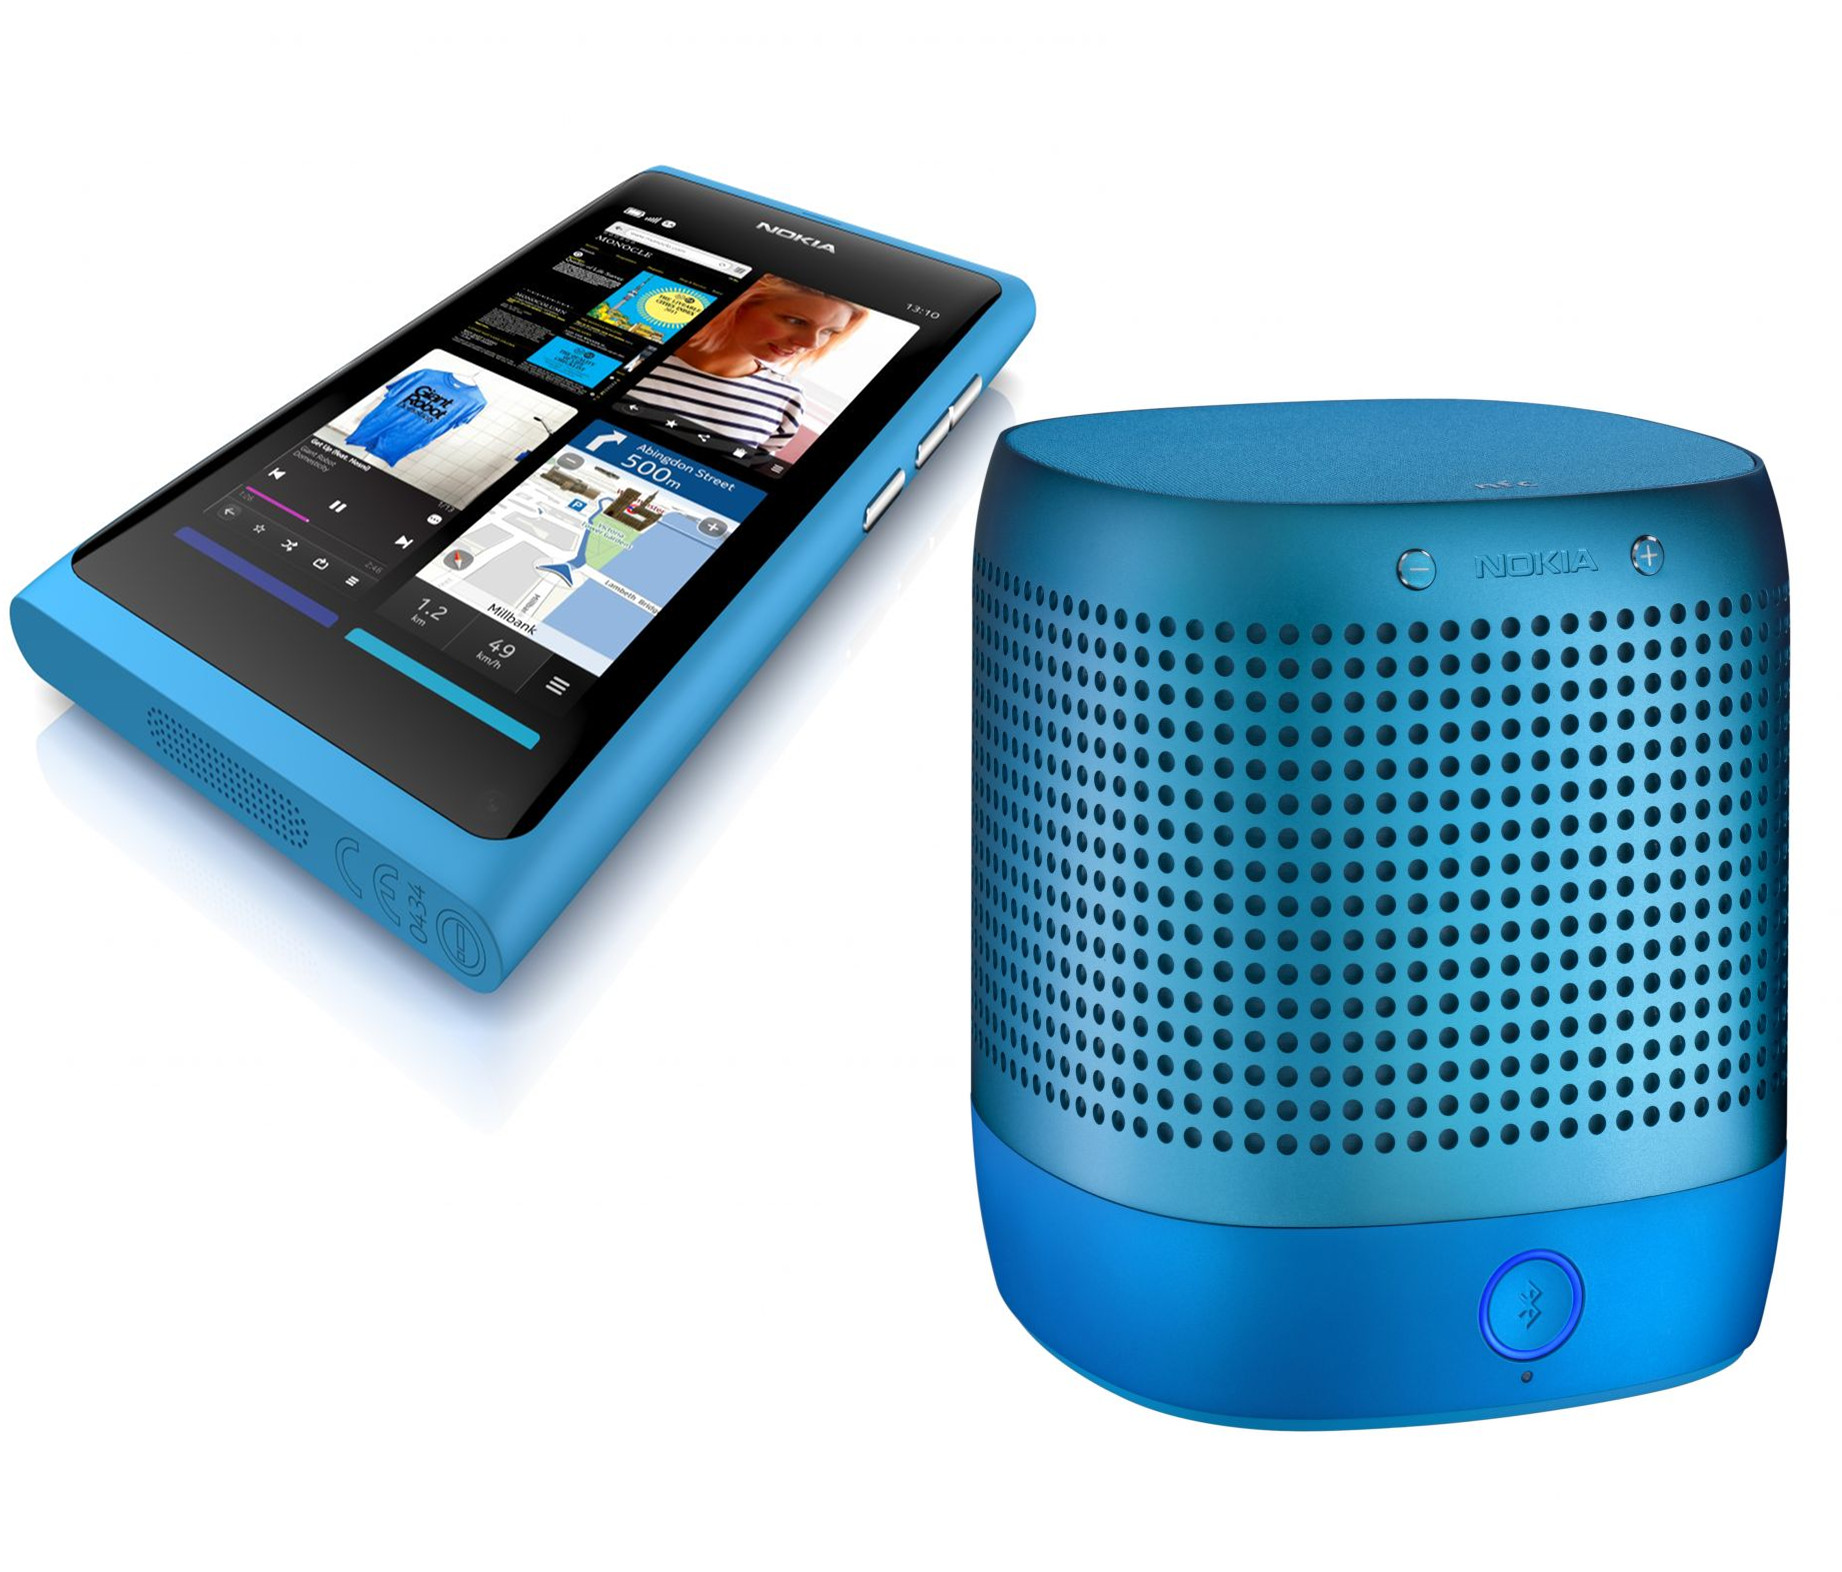
\includegraphics[width=\textwidth]{nokiaplayn9}
\end{center}
\caption{Nokia Play 360$^{\circ}$ speaker system and N9 mobile phone}
\label{nokiaplay}
\end{figure}


Another example of a meaningful connection is the Nokia Play 360$^{\circ}$ speaker system, shown in Figure \ref{nokiaplay}, where music can be streamed wirelessly to the speaker using an \ac{NFC}-enabled smart phone. By touching the phone to the top of the speaker, a connection is created that conceptually ``carries'' the music from the phone to the speaker.

The WiFi connection between a smart phone and a WiFi router is not a semantic connection, as the connection in itself has no clear meaning. A USB cable by itself is also not considered a semantic connection.

Semantic connections make up a structural layer of inter-entity relationships on top of the network architecture. These connections can be the real, physical connections (e.g. wired or wireless connections that exist between devices), or conceptual connections that seem to be there from a user's perspective. 
%The term ``semantic'' refers to the meaningfulness of the connections. We consider the type of connection, which currently often has the emphasis when interconnecting devices (e.g. WiFi, Bluetooth, USB) not to be the most relevant, but what the connection can do for someone---its functionality (e.g. stream music, share files)---even more.
Semantic connections exist in both the physical world and the digital domain. They have informative properties which are perceivable in the physical world. However, some of these physical qualities might be hidden by default, and only become visible on demand by means of a mediating interaction device. The digital parts of semantic connections are modelled in an ontology. There may be very direct mappings, e.g. a connection between two real-world entities may be modelled by a \texttt{connectedTo} relationship between the representations of these entities in an ontology. Sometimes the mapping is not so direct, for example where a semantic transformer is used. Semantic connections have several properties, which are explained in the following subsections. 

%The rationale behind Semantic Connections is to rely on:
%\begin{itemize}
%\item the meaning of existing objects to provide meaning for the relationships between the objects and the resulting meaning of the networked objects.
%\item the power of natural mapping and locality, using real objects and locations to provide meaning for the connections that are created between the objects and (object) locations.
%\item inherent, augmented and functional feedback and feedforward to strengthen the meaning of the connections and the emerging functionality \cite{Wensveen2004}.
%\end{itemize}

\subsection{Directionality}
\label{directionality}
As discussed in Section \ref{OntologyDesign3}, we consider a semantic connection to have a specified direction, or to be bidirectional/symmetric. Smart objects that are connected should then be identified as sources and/or sinks. Directionality may intentionally be specified through user action, or it can emerge from the capabilities of the smart objects e.g. connecting a source to a sink will automatically create a connection going from the source to the sink.

\subsection{Transitivity}
When connections have directionality and multiple devices (i.e. a minimum of three devices) are involved, devices can also act as bridges, transferring data due to transitivity. For example, if a music player is connected to speaker A, and speaker A is connected to speaker B, speaker A acts as a bridge between the music player and speaker B.

\subsection{Permanent and temporary connections}
Semantic connections can vary in persistence. Connections can be made during an interaction cycle involving several devices to transfer content or data from the one device to another, and the connection then stops existing when the interaction cycle is completed. Connections can also be used to configure more permanent information exchange between entities in a smart space, much like setting up a connection to a wireless network router. These permanent connections will persist, and will be automatically reconnected every time the smart objects that are connected co-exist in the same smart space.

\subsection{Connections connect different entities}
Connections can exist between smart objects, people and places. Not only objects and devices have meaning in a system of networked devices --- according to \cite{Poole2008} physical location within the home and device ownership (or usage) are of central importance for understanding and describing home networks by users. Ownership can be seen as a connection between a device and a person. Connections from and to places or locations can be seen as a way of structuring contextual information such as location. With very personal devices (such as smart phones and laptops or tablets) we can, when these devices are used in an interaction, implicitly infer the user's identity. With shared devices, we need a way to identify the user. In such cases, making explicit connections from the device at hand to something personal of the user (e.g. a phone or keychain) may be a way to indicate identity.


\section{Semantic Transformers}
\label{SemanticTransformers}

\marginpar{Semantic transformers were introduced in Section \ref{SemanticMediaOntology}.}
Semantic transformers were first defined in \cite{Niezen2011} as virtual entities that transform one type of information into another when a direct mapping is not possible. They transform user actions into interaction events and perform matching and transformation of shared data and content. Semantic transformers enable interoperability between devices by utilising device capability descriptions and content types to determine how devices may interoperate.

%To this end, the work done for touch and pen-tablet interaction by the recently established W3C Web Events Working Group was taken as a starting point \cite{w3c_wec}.

Semantic transformers can be used to map and transformed shared content between smart devices, for example a service that transforms a music stream into coloured lighting patterns that can be rendered by a lighting device. Semantic transformers can also be used to transform physical actions (such as pressing a button or performing a gesture) into representational events like adjusting the level of lighting in a room, or the adjusting the volume of a speaker. Semantic transformers may also be employed to perform simpler transformations such as inverting values. 

Physical identifiable objects are not considered semantic transformers and should rather be modelled as smart objects. Semantic transformers are services, and therefore have no physical appearance or tangible form. They can only be perceived through the smart objects they transform the information for. A semantic transformer is not considered a smart object, as it is a virtual object and not addressable in the physical environment.

% Possible TODO
%\subsection{Content flows: Streaming}
%	20/10/10, 18/11/10, 23-29/03/11, 12/04/11, 20/04/11, 03/05/11



% As a semantic transformer cannot have more than one functionality as input, we created an \ac{OWL} restriction\\
% 
% \noindent
% $\forall$~\texttt{SemanticTransformer}~$\sqcap$~\texttt{functionalitySource} = 1\\
% 
% Due to the \ac{OWA}, functionalities have to be defined as different (using \texttt{owl:allDifferent}) for the restriction to work.


%Niezen et al. \cite{Niezen2011} describe a semantic transformer as an entity responsible for interpreting data coming from different smart objects and data sources into possible user goals, and maps them onto the plurality of available services. This facilitates a paradigm change from today's function-oriented interaction to a future of goal-oriented interaction.

%Niezen et al. \cite{Niezen2011} describe a semantic transformer as an entity 

%User-action events are high-level input actions which capture and report the intention of the user's action directly, rather than just reporting the associated hardware input event that triggered the action. This high level of abstraction enables developers to write applications, which will work across different devices and services, without having to write specific code for each possible input device. The W3C Web Events Working Group defined four conceptual layers for interactions (for touch- and pen-tablet interaction) \cite{w3c_wec}:

%\begin{description}
%\item [physical] This is lowest level, and deals with the physical actions that a user takes when interacting with a device, such as pressing a physical button.
%\item [gestural] This is a middle layer between the physical and intentional, and describes specific mappings between the two; for example, a ``pinch'' gesture may represent the user placing two fingers on a screen and moving them together at the physical layer. This may map to a ``zoom-in'' event at the intentional layer.
%\item [representational] This is the highest level of abstraction in the event model, and indicates the means by which the user is performing a task, such as zooming in, panning, navigating to the next page, activating a control, etc.
%\item [intentional] This layer indicates the intention of the task a user is trying to perform, such as viewing more or less detail (zooming in and out), viewing another part of the larger picture (panning), and so forth.
%\end{description}
%
%\begin{table}
%\tbl{Examples of representational events in a smart environment \label{transformationTable}}{
%\centering
%\begin{tabular}{|l|l|}
%\hline
%Representational Event & Entity this event can be performed on\\
%\hline
%AdjustLevel & Volume, Lighting \\
%switchOnOff & Lighting, any SmartObject \\
%Navigate & Playlist, Menu, SequentialData \\
%Undo/Redo & Any interaction event \\
%Stop/Start & Application, Media \\
%DragAndDrop & Media \\
%Query & Media, other events \\
%\hline
%\end{tabular}}
%\end{table}
%
%In Table \ref{transformationTable} examples of possible representational events are defined. A representational event has more than one possible entity that it can be performed on, as well as more than one possible entity that triggers it, i.e., there exists some ambiguity. Only when no ambiguity exists as to which entity it is performed on, as well as the action which the user is trying to accomplish, we refer to it as an intentional event.
%Semantic transformations occur between physical actions (such as pressing a button or doing a gesture) and representational events, as well as between representational events and intentional events.

%end TiiS




\section{Finite state machine examples}
\label{fsmexample}
We now use \acp{FSM} to model and explain the different concepts introduced so far. \acp{FSM} allow us to talk about user interaction in a way that describes how users could think about user interaction, but that still makes sense to interaction programmers and designers \cite{Thimbleby2007}. The use of \acp{FSM} also encourages simplicity. 
% Turing machines and other sophisticated models of computing do not describe that what users think about.

As a first example, consider a simple light with an up/down switch as a single device (seen in Figure \ref{FSMsimple} on the left). There are two states (\texttt{On/Off}), an initial state (\texttt{Off}) and two events (\texttt{Switch\-Down\-Event/Switch\-Up\-Event}) that cause transitions between the states. If the switch is labeled, we can use more specific (meaningful) wording, for example \texttt{switch\-Off\-Event} instead of \texttt{switchDownEvent} (as shown in Figure \ref{FSMsimple} on the right). %(already defined as ODP:) We use the notation \texttt{[DeviceClass]} \texttt{[Action]Event} to define the interaction event - this makes them easier to classify into a hierarchical event structure.

\begin{figure}
\centerline{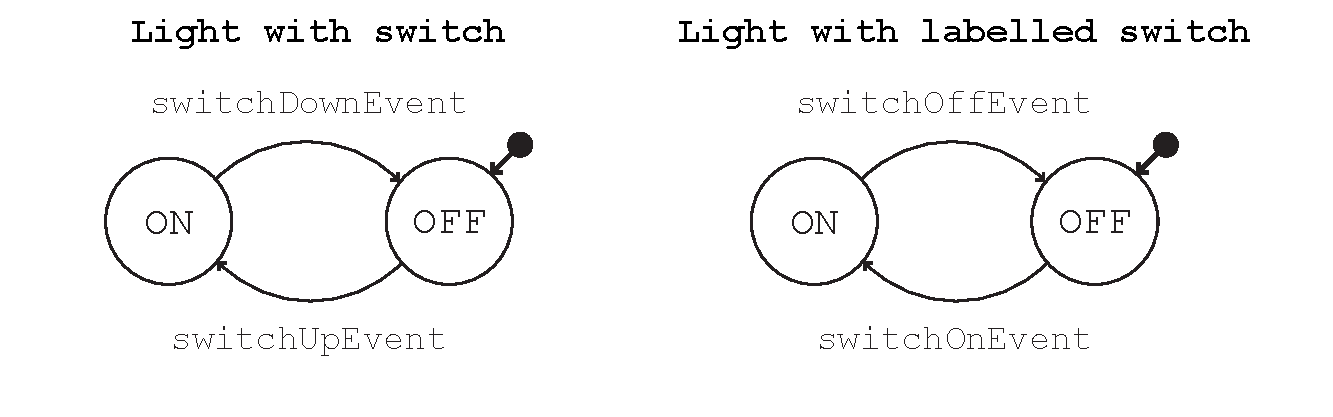
\includegraphics[width=\columnwidth]{FSMsimple}}
\caption{FSMs for a simple light with a switch and a light with a labelled switch}
\label{FSMsimple}
\end{figure}

\begin{figure}
\centerline{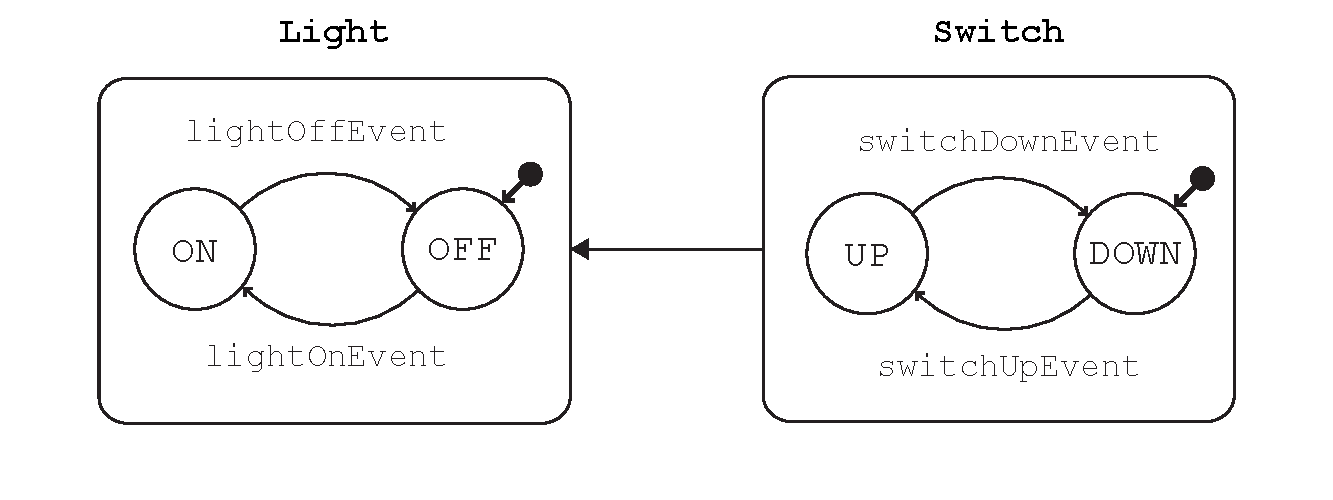
\includegraphics[width=\columnwidth]{FSMsmartObject}}
\caption{Light and light switch as two separate smart objects with a semantic connection}
\label{FSMsmartObject}
\end{figure}

In Figure \ref{FSMsmartObject} one of the simplest examples of a semantic connection is shown - a light (as a smart object) connected to a simple up/down switch (a second smart object). The light consists of two states (\texttt{On/Off}) with an initial (default) state of \texttt{Off}, and two events (\texttt{Light\-On\-Event / Light\-Off\-Event}) indicating the transitions between these states. Boxes with rounded corners are used to signify smart objects, while the semantic connection is indicated using a solid arrow point. Using arrows to denote semantic connections allows us to specify a direction for the connection. \marginpar{The concept of directionality was described in Section \ref{directionality}.} Note that the light has functional feedback, with perceivable light when it is switched on. The switch on the other hand has inherent feedback, with a perceivable \texttt{Up} or \texttt{Down} state.  

We can create mappings between the events to create an interaction path (see section \ref{interactionPath}), for example we use

\begin{quote}
SwitchUpEvent $\rightarrow$ LightOnEvent %: Default
\end{quote}

to indicate the most meaningful \emph{default} mapping. It should of course be possible to change this mapping, for example by using a semantic transformer that inverts mappings between devices.

\begin{figure}
\centerline{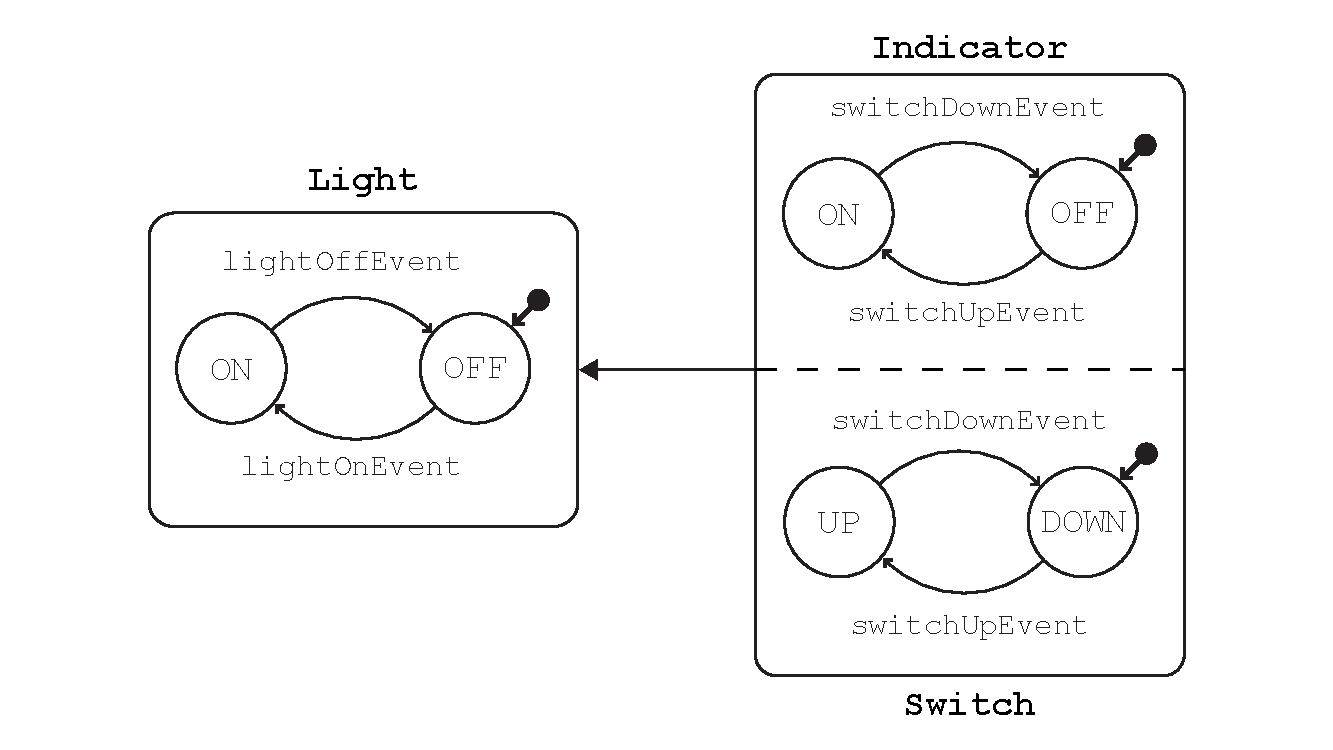
\includegraphics[width=\columnwidth]{FSMaugmentedFeedback}}
\caption{Light connected to light switch with augmented feedback}
\label{FSMaugmentedFeedback}
\end{figure}

In the case where a smart object is not in the same physical location as the smart object it is connected to, additional augmented feedback may be required. Consider the case where the light switch may be in a different room than the light - we could use an indicator on the switch to give augmented feedback to show whether the light actually switched on. This is shown in Figure \ref{FSMaugmentedFeedback}.

\begin{figure}
\centerline{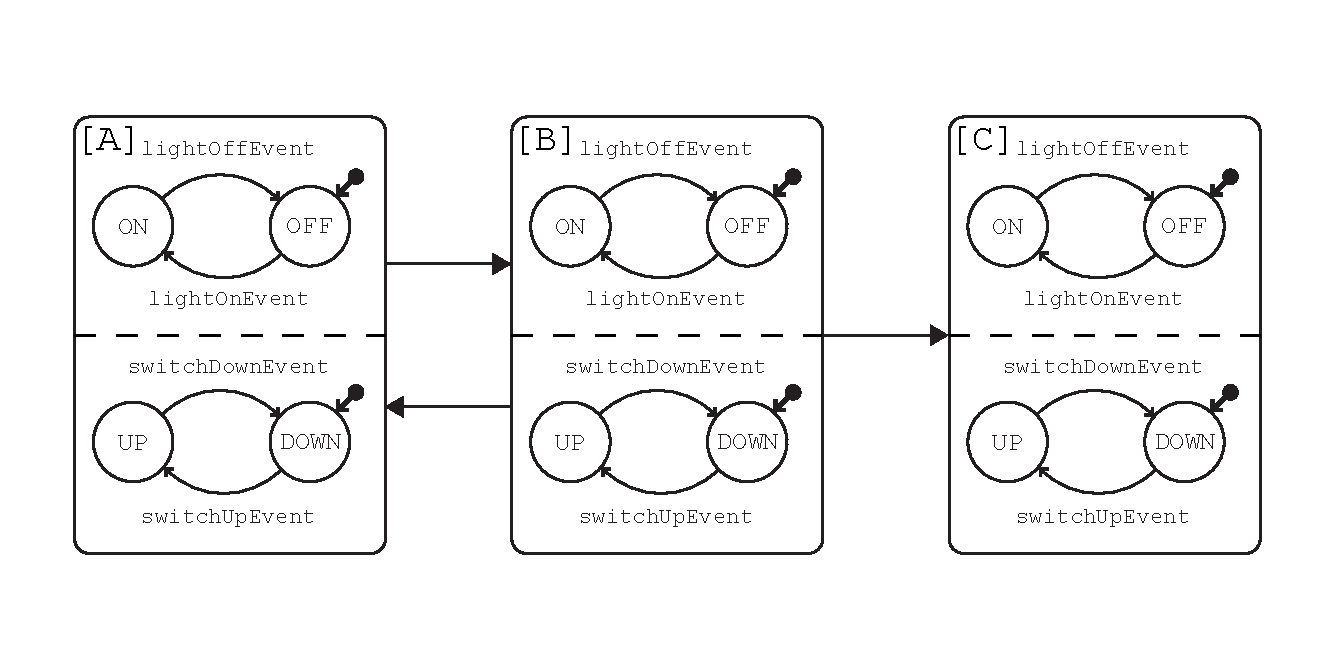
\includegraphics[width=\columnwidth]{FSMsymmetry}}
\caption{FSM showing semantic connection with symmetry}
\label{FSMsymmetry}
\end{figure}

%what about the concept of directionality itself?
A more complex example is shown in Figure \ref{FSMsymmetry}. In this example there is a symmetric (bidirectional) connection between smart object A and B, with the result that pressing the switch on smart object A will turn the light in smart object B either on or off, and vice versa, B will control A. Since B is connected to C, actions on A and B, will also be reflected on C. On the other hand, pressing the switch of C will have no effect on either A or B. Due to the symmetric connection, we expect A and B to be in an identical state. How exactly this is implemented is up to the designer. \marginpar{One possible solution for such a light switch is a push button with an indicator light, such that the switch able to change its state by itself.}
%how does this exactly work with tactile switches with an up/down position, does the switch always change the current state of the connected lights? What about a situation where a physical switch is in an "open" position, and the light is off? does it change the position of the switch? G: I think we consider a smart light switch to not have a permanent "open" position, where the indicator will turn off if the light is off (the position doesn't indicate the state), and the switch will always change the state when pressed.

\begin{figure}
\centerline{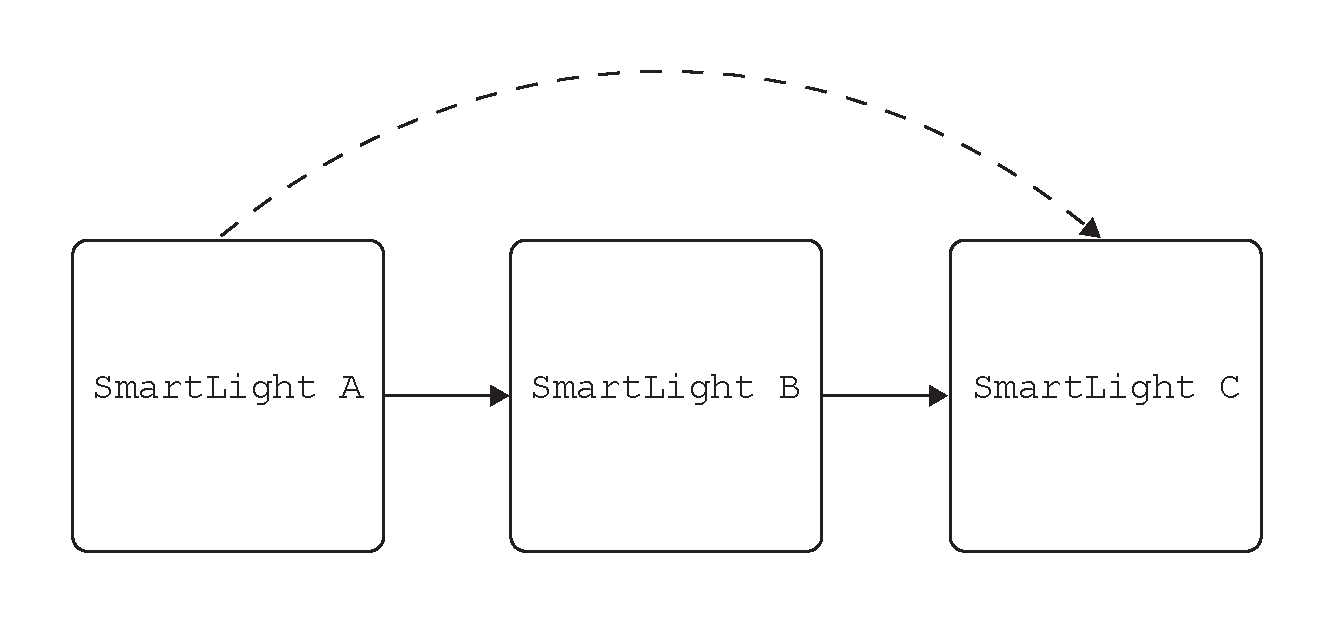
\includegraphics[width=300px]{FSMtransitivity1}}
\caption{FSM showing a semantic connection with transitivity}
\label{FSMtransitivity}
\end{figure}

In Figure \ref{FSMtransitivity} we use the SmartLight abstraction to denote the FSM of a smart light as shown in previous figures. When SmartLight A is connected to SmartLight B, and in turn is connected to C, transitivity allows us to infer a direct connection (indicated by a dashed arrow) between A and C. Pressing the light switch on A will in this case affect both B and C.

\begin{figure}
\centerline{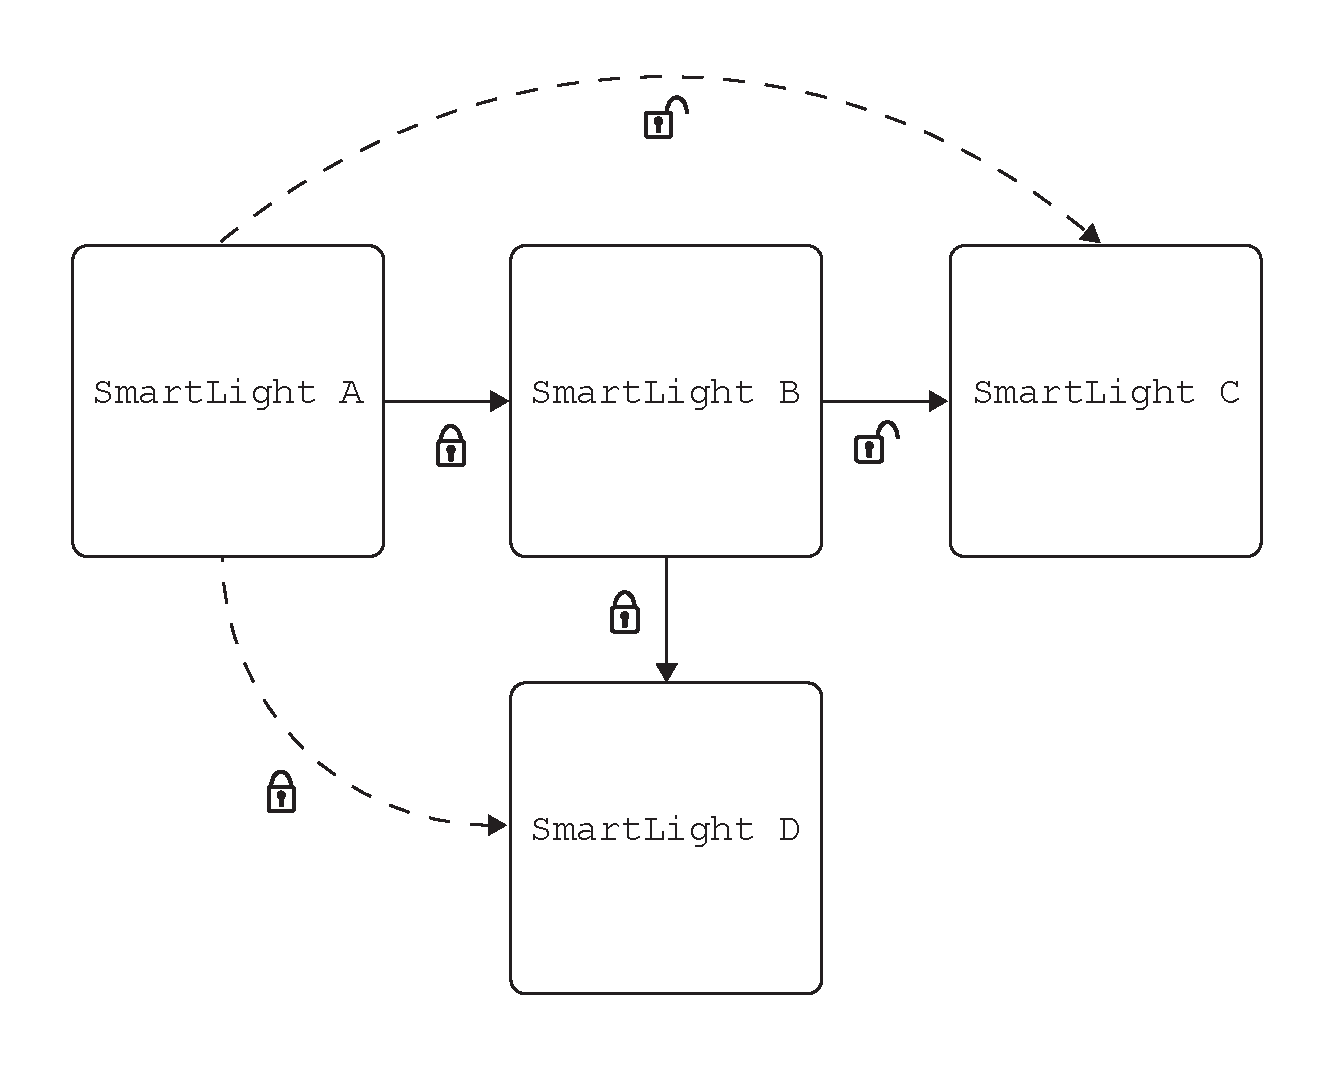
\includegraphics[width=300px]{FSMpersistence}}
\caption{FSM showing a semantic connection with transitivity and persistence}
\label{FSMpersistence}
\end{figure}

We use locked/unlocked icons next to semantic connections to indicate persistence (see Figure \ref{FSMpersistence}). The locked icons between A, B and D indicate persistent connections between those objects, and a persistent transitive connection is then inferred between A and D. This means that if smart object D moves to another location, all three connections (including the A$\rightarrow$D connection) continue to exist. The connection between B and C is temporary, which means that the inferred transitive connection between A and C is also temporary. If smart object C moves to another location, both the B$\rightarrow$C and A$\rightarrow$C connections will be removed.

\begin{figure}
\centerline{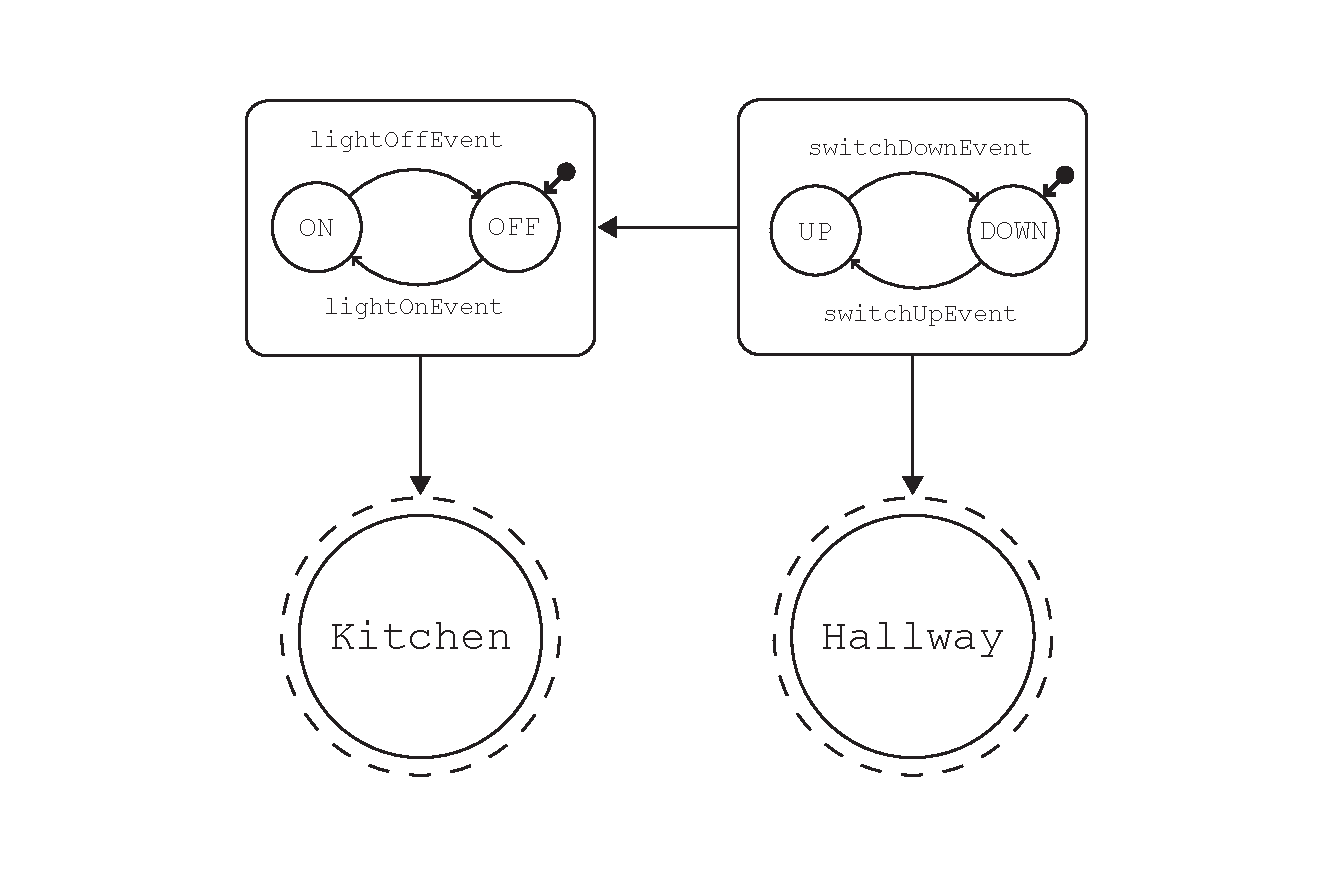
\includegraphics[width=\columnwidth]{FSMplaces}}
\caption{FSM showing semantic connections between smart objects and places}
\label{FSMplaces}
\end{figure}

In Figure \ref{FSMplaces} we show semantic connections between smart objects and specific locations, where the dashed-double circle denotes a location. This places semantic connections between places and objects on the same abstraction level. We use semantic connections between smart objects and places as a way to structure relevant contextual information. In our example in Figure \ref{FSMplaces} we cannot infer that a user actually is able to observe the functional feedback of switching the light on and off, as they are not located in the same space, and might not be able to see the light. The importance of feedback and feedforward and how they should be handled between different locations is described in more detail in section \ref{section:feedbackAndFeedforward}.

\begin{figure}
\centerline{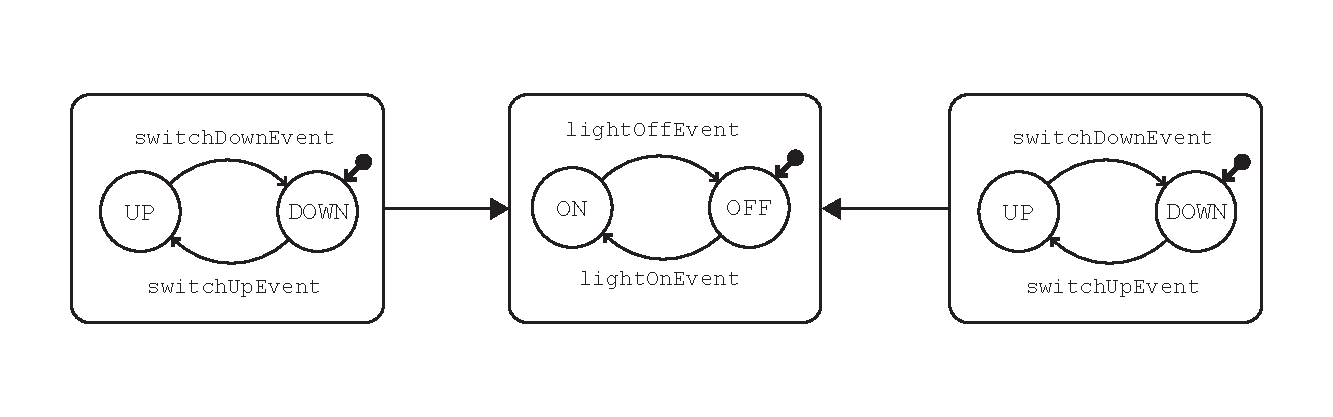
\includegraphics[width=\columnwidth]{FSMpriority}}
\caption{FSM showing a situation where priority is an issue}
\label{FSMpriority}
\end{figure}

When two switches are connected to the same light as is shown in Figure \ref{FSMpriority}, the issue of priority arises. We define the most meaningful default to be that the last event that occurred has priority. In Figure \ref{FSMpresence} where the one interaction is incidental, generated by a presence sensor, and the other is intentional (as described in Section \ref{intentionalSpectrum}), the intentional interaction takes priority.

\begin{figure}
\centerline{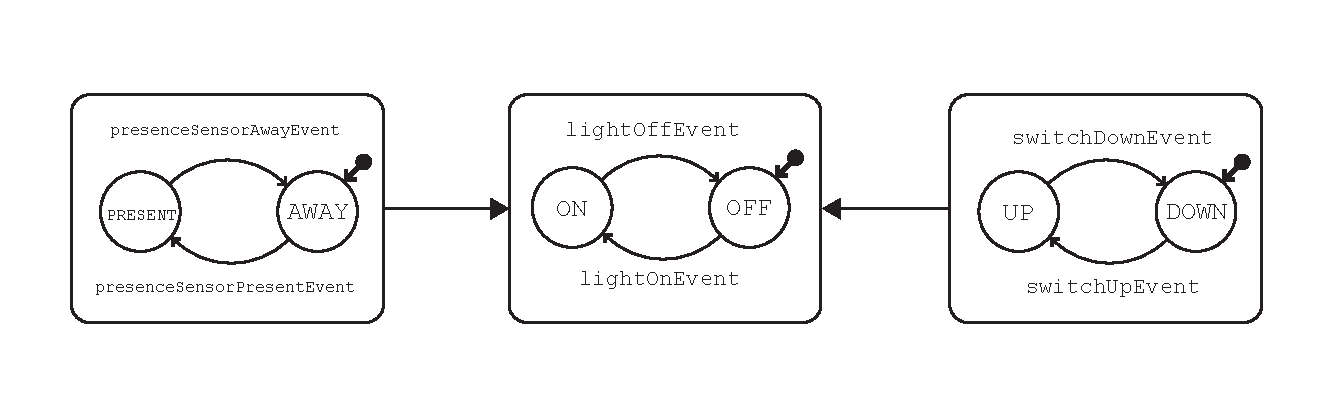
\includegraphics[width=\columnwidth]{FSMpresence}}
\caption{FSM showing incidental (presence sensor) and intentional (light switch) interactions}
\label{FSMpresence}
\end{figure}


\section{Feedback and feedforward}
\label{feedbackforward}
If we view our concept of semantic connections in terms of the Interaction Frogger framework (as discussed in Section \ref{interactionFrogger}), the following interesting insights emerge.

\subsection{Feedback of objects}
When we consider multiple interconnected smart objects and the functionalities and services they provide, information like feedback and feedforward gets spatially distributed. A user may operate a device, receiving inherent feedback locally, but receiving augmented and/or functional feedback remotely. 

As inherent feedback is inherent to the operational controls of the device, these reside only in the physical world and are local to the device. We thus do not model this feedback in the digital domain. Augmented feedback is feedback that is augmented from the digital domain onto the physical world. This type of feedback is subject to change when devices are connected to other devices. In the domain of networked digital artefacts, functional feedback is of a digital nature. Data, media and services that exist in the digital domain become available in the physical world, through the various devices and their connections. In Figure \ref{model}, the several types of feedback are indicated. 

Although many functionalities of digital devices can be regarded as displaying media, data or services, for some simple functionalities this seems problematic. If we, for example, look at functional lighting, it seems that the presence of light as the functionality of a lighting device is not a concept that is part of the digital domain. However, if we view a lighting device as a networked smart object, the presence of lighting, based on some sensor data, can be regarded as the functionality of a digital service.\marginpar{Refer to Van der Vlist's thesis \cite{Bram} for more detail on how the theory of product semantics can be applied to feedback and feedforward.}

% As mentioned before, semantic connections (potentially) \emph{change} functional and augmented feedback and its location. Additionally, semantic connections themselves show feedback as well, when users interact with them through an interaction device. 

\subsection{Feedback of connections}

Inherent feedback becomes feedback that is mediated through an interaction device used to make or break the connection, as one can not manipulate a wireless connection directly. This inherent feedback may however be closely related to the action of making or breaking a physical connection, like a snap or click when the connection is made or broken. Augmented feedback to indicate a connection possibility or an existing connection may be in the form of lights, or in the form of projected or displayed lines. Functional feedback is information about the actual function of the connection, like music playback from a speaker that was just connected to a media player. This type of feedback always reaches the user through the devices being connected. 

\subsection{Feedforward}
Inherent feedforward, conceptually similar to the notion of affordances  \cite{Norman1998}, provides information about the action possibilities with the devices or the individual controls of an interface. Inherent feedforward is always physical and local on the device. However, when devices or objects are part of a larger system, feedforward also emerges where interaction possibilities between objects exist (e.g. a key that fits a lock, a connector of one device or cable that fits another). The same holds for augmented feedforward, where lights, icons, symbols and labels provide additional information about the action possibilities. These may concern the action possibilities locally at the device, as well as action possibilities that concern the interaction with other devices in the environment. 

While inherent and augmented information are primarily concerned with ``the how'', functional feedforward communicates ``the what'', the general function of the device or the function of a control. This type of information often relies on association, metaphors and the sign function of products, and are described in theories such as product semantics and product language. With multifunctional devices, and even more with smart objects, this becomes increasingly difficult. Introducing the concept of semantic connections tries to address these problems, therefore the functional feedforward is the main challenge when designing semantic connections. Functional feedforward gives information about the function of the semantic connection before the interaction takes place. Properly designing functional feedforward is therefore the crucial part of understanding semantic connections, smart services and smart environments.\marginpar{An example of where functional feedforward was used in the third design iteration is described in Section \ref{section:feedbackAndFeedforward}.}

Wensveen \cite{Wensveen2004} further proposes that in interaction, these types of information can link action and function together in time, location, direction, modality, dynamics and expression. Strengthening these couplings between action and function will lead to richer and more intuitive interactions \cite{Wensveen2005}.
 
We can also view semantic connections in the Frogger framework in more general terms. Although semantic connections are not a physical device or product, but rather describe the structure or configuration of a system of devices, the Frogger framework can teach us important lessons. When we look at the link between action and functional information in time or location, a strong link would mean they coincide in time and location. For location this would mean that the connection that is made between devices corresponds to the location of the actual devices in physical space. But also that the feedback that is provided is coupled to the action in time an location. Additionally, the direction of the action of connecting/disconnecting devices, being moving devices towards or away from each other, strengthens the coupling in terms of direction. Also, the direction of the action could have a link to the directionality of the semantic connection that is made (e.g. the order in which endpoints of a connections are defined). Couplings in dynamics (of the action) can be used in similar ways and may express the persistence of the connection that is made. 



\section{Discussion \& Conclusion}

In this chapter we introduced our Semantic Connections theory and used finite state machines to model and explain the different concepts. We defined the following main concepts: 

\begin{itemize}
	\item Smart objects, and the means to describe them in terms of a unique physical and digital identity
	\item Interaction primitives, and how they can be used to describe the user interaction capabilities of smart objects
	\item Semantic connections, and how they can be used to model meaningful connections between smart objects
	\item Semantic transformers, and how they transform information from one type into another
\end{itemize}   %We showed that, even when important interaction events are shared between smart objects, state misalignments will occur. Good practice is to share all important user interaction events and events that cause state changes that are prominently perceivable by users. Using finite state machines to understand such behaviour helps to achieve this.

We identified some of the principles of semantic connections, including directionality and transitivity, as well as permanent and temporary connections. We also identified principles of the various types of feedback and feedforward that are required, not only for connections but also for smart objects.

The importance of being able to uniquely identify smart objects in both the physical and digital space, as well as sharing their interaction capabilities and states, was shown, including how it was grounded in the theory of interaction models by Nielsen, Card and others.

% In our theory we describe semantic connections as meaningful relations that can exist, not only in between smart objects, but also between smart objects, people and places. Although we still believe this is interesting to consider, this did not form part of the actual implementation. It may be interesting for future work, including e.g. relationships between persons (digitally described in social networks) and investigate whether these different types of relationships should be transitive as well (e.g. person A is friends with person B, person A owns device \texttt{a}, and B owns device \texttt{b}, should we infer friendship between \texttt{a} and \texttt{b}? Or, when device \texttt{a} is in the same room as device \texttt{b} and they are touched together, is it safe to infer data can be exchanged over a connection established without passwords? 

We showed how augmented and functional feedback and feedforward can help users to better predict the functional result of the connections they create. Functional and augmented feedback also showed to be key in maintaining the causal links between user action and function, distributed over interconnected smart objects.

A fundamental difficulty encountered during the implementation of the feedback and feedforward (and which is also a big challenge in interoperability in general), is what we call the \emph{awareness paradox}. To foster emergent functionality, efforts are aimed at enabling smart objects to interoperate without their combined functionality being specifically designed. This means that the smart objects are unaware of each other, exchanging information though an information broker. For the users however, it is imperative that smart objects show behaviour as to appear to be aware of each another. 

The way out of the paradox is to make use of proper use of feedback and feedforward that can be generated  at runtime. Since the connections that may be created during use are not known at design time, smart decisions have to be made on how to describe the interaction events and functionalities that are shared. 

By describing feedback and feedforward of the semantic connections as a result of the match in capabilities and functionalities, and having the semantic transformers and sink objects (instead of the source) produce the preview and indicator feedback, we make sure that they are capable of displaying (i.e. in the widest sense of the word, not limited to the visual modality) this feedback. Our reasoning is that, if a sink can be the sink of a functionality, it should also be capable of giving feedforward and feedback for this functionality.\marginpar{Examples of preview events were shown in Chapter \ref{DesignIteration3}.}

%perhaps the simple examples of the awareness of a presence sensor connected to a light. and/or a more complex example with feedback/feedforward.

Moreover we showed that semantic connections and using semantic transformers to create services is an appealing idea, leading to additional and, more importantly, more meaningful functionalities of ensembles of existing devices. This may reduce the number of devices needed in our daily lives by reducing redundant devices.

%After we implemented our theory we feel more confident that we defined a complete set of entities and properties to achieve our goal of creating interoperability between smart objects and to enable users to interact with the objects and the relationships between them at a semantic level. Even though our theory describes how to implement smart objects and provides the necessary core ontology, we believe enough freedom remains for designers and developers to create their own unique objects and interactions. %examples

Our Semantic Connections theory provides a foundation for modelling user interactions with interoperating smart objects in smart environments, and therewith the possibility to improve the interoperability among them. We considered the notions of feedback and feedforward to enhance perception of connectivity and the perceived causality between user action and feedback.   

In the next part of the thesis, we will look at other concepts and techniques that can be used in smart environments, like device capability modelling and event modelling. Similarly to how we extracted the theory of semantic connections from the work completed in the design iterations, these more general concept and techniques are also based on the work done during the three design iterations.

% Summarising, we made the following observations and changed and/or added to the theory accordingly:
% 
% \begin{itemize}
% \item 	we refined the definition of smart objects; 
% \item 	we refined the definition of semantic transformers and the connections between smart objects and semantic transformers;
% \item 	we implemented direction in the semantic connections and observed its implications on information flow and user interaction;
% \item 	with the directionality and transitivity, smart objects are defined as sources, sinks and bridges, semantic transformers can also be bridges;
% \item 	we implemented augmented and functional feedback and feedforward, introducing \texttt{PreviewEvents} and \texttt{IndicatorEvents}; and
% \item 	we implemented  temporary connections between the connector and smart objects (defining a Connector object as a smart object itself).
% \end{itemize}

% With regards to feedback and feedforward, we made important steps towards defining how this important information is changed when devices are considered in a system of networked objects as opposed to the devices in isolation. We believe that our theory may help other interaction designers and developers to deal with design opportunities and challenges that emerge when designing for interoperability.

%end TiiS


% Possible TODO \section{Interaction primitives}
% 24/08/10, 26/08/10, 27/08/10
% InputToAction: 06/10



\cleardoublepage
\ctparttext{In this part of the thesis, the more general concepts and techniques that can be applied to ubiquitous computing are described. These concepts and techniques were extracted from work done during the three design iterations.}
\part{Generalised models, software architecture and evaluation}
\chapter{Device capability modelling}
\label{DeviceCapabilityModelling}

\begin{flushright}{\slshape    
Whenever we capture the complexity of the real world in \\
formal structures, whether language, social structures, or \\
computer systems, we are creating discrete tokens for \\
continuous and fluid phenomena. In doing so, we are bound \\
to have difficulty. However, it is only in doing these things\\
 that we can come to understand, to have valid discourse,\\
 and to design.} \\ \medskip
    ---  Alan Dix
\end{flushright}


%\section{Describing devices: Device modelling}
%CC/PP, UAProf, FIPA
%While it is possible to determine a device's capabilities from its information shadows \cite{OReilly2009}, the capabilities modelled in the smart space are only those which are meaningful to share. 
%- dcs ontology
%- UWA, Delivery Context Ontology (relates to UAProf)

In order to share device capabilities with other devices in the environment, we require ways to describe these capabilities. While we have touched lightly on some of the techniques in the thesis so far, this chapter will focus in more detail on the current state-of-the-art, as well as how we extended these techniques to create a new way of modelling device capabilities using ontologies.

Most of the existing work on modelling interaction capabilities focuses on \ac{GUI} based techniques. 

\section{GUI-based techniques}

A \emph{universal user interface language} describes user interfaces that are rendered by mapping a description's device-independent interaction elements to a target platform's concrete interface objects \cite{Lee2006}. This allows developers to create the user interface in an abstract language without targeting a specific device. Examples of interface languages include \ac{UIML}, \ac{XIML}, Carnegie Mellon University's  \ac{PUC} and the \ac{INCITS/V2 URC}. These languages allow devices to determine the most suitable presentation based on a predefined set of abstract user interface components.

\ac{UIML} maps interface elements to target UI objects using a styling section, resulting in one styling section per target device type. However, it does not include a vocabulary to describe more abstract widgets \cite{Zimmermann2007}. \ac{PUC} describes device functions in terms of state variables and commands, with a grouping mechanism used for placement of UI objects. The \ac{INCITS/V2 URC} standards define a generic framework and an XML-based user interface language to let a wide variety of devices act as a remote to control other devices, called targets.

\emph{User interface remoting} uses a remote interface protocol that relays I/O events between an application and its user interface. The user interface resides on a remote platform instead of on the device itself. The \ac{UPnP} \ac{RUI}, that forms part of the \ac{UPnP} AV standard,  belong to this category. \ac{UPnP} \ac{RUI} follows the Web server-client model, where the controller acts as a remote user interface client, and the target, acting as a remote user interface server, exposes a set of user interfaces \cite{UPnPForum}.

CEA-2014, that builds on the \ac{UPnP} \ac{RUI} interface, uses a matchmaking process for a controller device to select a user interface protocol that is supported by the controller platform \cite{Zimmermann2007}. Supported protocols include AT\&T \ac{VNC} and Microsoft \ac{RDP}. \ac{VNC} uses the \ac{RFB} protocol to send pixels and event messages between devices. 

Universal user interface languages and user interface remoting are orthogonal approaches \cite{Lee2006}. User interface remoting might be used in parallel with device-independent user interface languages.

%\marginpar{Current remote user interfaces are device-oriented rather than task-oriented. CEA-2018, discussed earlier in Section \ref{cea2018}, tries to solve this problem by using task model representations.}



% Lee2006 also describes uJuni and INCITS / V2 URC

In this thesis we are more interested in tangible interactions in ubiquitous computing environments, instead of the usual \ac{GUI}-based solutions. Smart environments need not only descriptions of \ac{GUI}-based input/output, but also descriptions of the physical input/output capabilities, hardware capabilities, network capabilities and other characteristics of smart objects. The first attempt to define a vocabulary that conveys these device characteristics was the W3C \ac{CC/PP}\footnote{http://www.w3.org/Mobile/CCPP/}. Other approaches to describe device characteristics that are not \ac{GUI} specific are described in the next section.

\section{Non-GUI techniques}

\subsection{UAProf}

The WAP Forum's \ac{UAProf} specification is an \ac{RDF}-based schema for representing information about device capabilities.\marginpar{W3C's \ac{CC/PP} is also an \ac{RDF}-based schema.} UAProf is used to describe the capabilities of mobile devices, and distinguishes between hardware and software components for devices.

%start africon
%The User Agent Profile (UAProf) specification, used to describe the capabilities of mobile devices, distinguishes between hardware and software components for devices, but the descriptions of interaction capabilities are very limited. 

For example, in the Nokia 5800 XpressMusic UAProf profile\footnote{nds1.nds.nokia.com/uaprof/Nokia5800d-1r100-2G.xml
}, its interaction capabilities are described as follows:

\begin{itemize}
	\item \texttt{PhoneKeyPad} as \texttt{Keyboard}
	\item 2 as \texttt{NumberOfSoftKeys}
	\item 18 as \texttt{BitsPerPixel}
	\item 360x640 as \texttt{ScreenSize}
	\item Stereo as \texttt{AudioChannel}
\end{itemize}

Other user interaction capabilities are defined in a Boolean fashion of yes/no, e.g. \texttt{SoundOutputCapable}, \texttt{TextInputCapable}, \texttt{Voice\-Input\-Capable}.
%end africon

\subsection{Universal Plug and Play (UPnP)}
\label{UPnP}

\ac{UPnP} with its device control protocols is one of the more successful solutions\footnote{http://upnp.org/sdcps-and-certification/standards/sdcps/} to describing device capabilities. However, it only allows for the definition of one level of tasks \cite{Niezen2010}.

\ac{UPnP} was developed to support addressing, discovery, eventing and presentation between devices in a home network, and the current version (1.1) was released as the ISO/IEC 29341 standard in 2008. It consists of a number of standardised \acp{DCP} - data models that describe certain types of devices. The \acp{DCP} that have been adopted by industry include audio/video, networking and printers. \acp{DCP} for low power and home automation have not yet been adopted.

\ac{DLNA} is a complete protocol set around \ac{IP} and \ac{UPnP}, where to be certified for \ac{DLNA}, a device needs to have \ac{UPnP} certification first. This protocol set was developed mainly to increase interoperability between \ac{AV} equipment in the home. It achieves this by limiting the amount of options available in the original protocol standards.\marginpar{In an IEEE ComSoc online tutorial entitled \emph{Consumer Networking Standardizations}, Frank den Hartog from TNO stated that ``DLNA has been a major effort to get computer people to talk to consumer electronics people''.}

When describing the capabilities of a smart object, not only the interaction capabilities are important, but also the device states. With \ac{UPnP}, two types of documents are used to describe device capabilities and states. A \emph{device description document} describes the static properties of the device, such as the manufacturer and serial number \cite{Jeronimo2009}. \ac{UPnP} describes the services that a device provides in \emph{service description documents}. These XML-based documents specify the supported actions (remote function calls) for the service and the state variables contained in the service. 

The state variable descriptions are defined in a similar way to how we define our interaction primitives, with a unique name, required data type, optional default value and recommended allowed value range. The \ac{UPnP} Forum has defined their own custom set of data types, with some similarity to the XML Schema data types used by \ac{OWL} 2. As an example, consider a state variable to describe the darkness of a piece of toast, where \texttt{ui1} is defined as an unsigned 1-byte integer:

\begin{minted}{xml}
	
<stateVariable sendEvents="no">
	<name>darkness</name>
	<dataType>ui1</dataType>
	<defaultValue>3</defaultValue>
	<allowedValueRange>
		<minimum>1</minimum>
		<maximum>5</maximum>
		<step>1</step>
	</allowedValueRange>
</stateVariable>

\end{minted}

The \texttt{sendEvents} attribute is required for all state variable descriptions. If set to \texttt{"yes"}, the service sends events when it changes value. Event notifications are sent in the body of an HTTP message and contain the names and values of the state variables in XML. 

Let us consider these device states in terms of user interaction. There are four key concepts in an interaction - actions, states (internal to the device), indicators, and modes (physically perceivable device states) \cite{Thimbleby2007}. The user performs actions, which change the device state, which in turn control indicators (augmented feedback). Users may not know exactly which state or mode a system is in. \marginpar{Our approach to modelling devices states and state transitions using \acp{FSM} is described in Section \ref{fsmexample}. } If we want to fully capture the capabilities of the device, we need to specify the device states, the transitions between these states, the interaction primitives which can cause these state changes, as well as the default and current states of the device. When this device is then connected to another device, we also need a way to communicate state changes to the other device.


%end TiiS


\subsection{SPICE DCS}
\label{spice}
The \ac{SPICE} Mobile Ontology\footnote{http://ontology.ist-spice.org/} allows for the definition of device capabilities in a sub-ontology called \ac{DCS} \cite{Villalonga2009}. A distinction is made between device capabilities, modality capabilities and network capabilities. While the ontology provides for a detailed description of the different modality capabilities, e.g. being able to describe force feedback as a \texttt{Tactile\-Output\-Modality\-Capability}, there are no subclass assertions made for other device capabilities. Most physical characteristics of the devices are described via their modality capabilities, e.g. a \texttt{screenHeight} data property extends the \texttt{VisualModalityCapability} with an integer value, and the \texttt{audio\-Channels} data property is also related to an integer value with \texttt{Acoustic\-Modality\-Capability}. The input format of audio content is described via the \texttt{AcousticInputModalityCapability} through an \texttt{inputFormat} data property to a string value.

%It is not clear whether the modality capabilities should be used to describe the actual content that may be exchanged or the user interaction capabilities. As an example, if a device has an \texttt{Acoustic\-Output\-Modality\-Capability}, it is not clear whether the device can provide user interaction feedback (e.g. in the form of computer-generated speech or an audible click), or that the device has a speaker.




\section{Registering devices on startup}

Based on this existing work, we now look at our approach to registering device functionalities, as well as how we identify devices in the digital and physical domain.

On device startup, the smart object registers its digital and physical identification information (e.g. RFID tag or IP address) and its functionality with the SIB, and then subscribes to new connections and events as shown in Figure \ref{connectorsibSequence}.

\marginpar{The startup sequence contains instances of the blackboard and publish/subscribe patterns described in Section \ref{pubsubblackboard}.}
\begin{figure}[bth]
\begin{msc}
msc {
	//hscale = "1.5";
	
    A [label="Smart Object A"],sib [label="SIB"], connector [label="Connector Object"]; // B [label="Smart Object B"];
	A->sib [label="Register identification info"];
	A->sib [label="Register functionality"];
    A->sib [label="Check for existing connections"];
    --- [label="If connection exists", ID=1];
    sib->A [label="Connection exists to B"];
    A->sib [label="Subscribe to source events"];
    --- [label="End if", ID=1];
    A->sib [label="Subscribe to connection changes"];
    A=>A [label="Waits for new event or connection"];
    connector->sib [label="New connection from B to A"];
    sib->A [label="New connection"];
    A->sib [label="Subscribe to source events from A"];
    A=>A [label="Waits for new event or connection"];
    connector->sib [label="Connection removed from B to A"];
    sib->A [label="Connection removed"];
    A->sib [label="Unsubscribe from source events"];
    A=>A [label="Waits for new event or connection"];
}
\end{msc}
        \caption{Startup sequence between smart object and SIB}
        \label{connectorsibSequence}
\end{figure}

This sequence is the same for all smart objects that connect to the \ac{SIB}, and should be implemented in every \ac{KP} that uses our approach. You might notice some parallels between the concept of a \ac{SIB} and the Microsoft Windows Registry. The Registry is used to store configuration information of software applications on a single device, while the \ac{SIB} is used (among other things) to store device functionality descriptions of a system of devices. However, compared to the Windows Registry, which is a basic hierarchical key-value store, the triple store and reasoning engine used in the \ac{SIB} provide a number of advantages, including subsumption testing, consistency checking and the ability to use restrictions to constrain data instances.\marginpar{Subsumption testing, consistency checking and restrictions are discussed in more detail in Section \ref{owlreasoning}.} This means we can use reasoning to verify the consistency and stability of the data in the \ac{SIB}.

We now discuss the first two steps of the sequence diagram in Figure \ref{connectorsibSequence}, registering identification and functionality, in more detail.

\subsection{Identifying devices}

In order to discover a device's capabilities, it is first necessary to be able to uniquely identify the device. Today it is common to identify groups of products using barcodes and other numbering systems. Before ubiquitous computing, only expensive things such as precious metals, currency, or large machines were individually identified with any regularity \cite{Kuniavsky}. New tracking technologies like \ac{RFID} tags and smart cards allow us to link a unique identification number to a specific physical product, like a smart phone that identifies a specific person to the phone network. IPv6, an extension to the Internet Protocol standard, allows us to identify approximately $3.4 \times 10^{38} $ objects in the digital domain.

% The significance of technologies like \ac{RFID} is that they offer a way to endow physical objects with an \emph{information shadow} \cite{Greenfield2006}. An information shadow describes the digital information that is tied to a specific product. \marginpar{Amazon.com for example, use their \ac{ASIN} to uniquely identify every product they sell.} In Bruce Sterling's book about ubiquitous computing and design, Shaping Things \cite{Sterling2005}, he uses the example of a wine bottle to describe these kinds of objects. 
% 
% Wine bottles have easily findable identifiers that link to their information shadows, usually consisting of a large amount of user-generated content. In addition to the metadata that is on the label, like the year when it was bottled, or the grapes that were used, information shadows provide information ``about the people and processes that made the bottle and its contents''. He argues that the wine's carefully designed information aspects, like the web page and bar code, permanently change people's relation to wine. The question now becomes: How do create and link these physical and digital identities in ubiquitous computing environments?

% Possible TODO "unique naming" papers on Mendeley

Mavrommati et al \cite{Mavrommati2004} linked an XML-based description of an object's properties, services and capabilities with an artefact ID. This alphanumeric ID is mapped to a namespace-based identification scheme, using a similar process to the one used for computer MAC addresses.

Tungare et al \cite{Tungare2007} identified an information object in their Syncables framework, used to migrate task data and state information across platforms, via a \ac{URI}. They used the structure 

\begin{verbatim}
sync://<info-cluster-id>/<collection>/<type>/<path>/<object-name>	
\end{verbatim}

where the information cluster is the set of all devices a user interacts with during the course of a day. Each of the devices in an information cluster ``offers a unique set of affordances in terms of processing capabilities, storage capacities, mobility constraints, user interface metaphors, and application formats''.

Most service discovery mechanisms, for example those used by \ac{UPnP}, assume the user will use the Internet to establish connections \cite{Jeronimo2009}. However, when we are in close proximity to things, we can address these things by pointing at them, touching them or by standing near them, instead of having to search or select them through a \ac{GUI}.

Olsen et al. \cite{Olsen2001} used the domain name or IP address of a software client associated with a device to identify it, and a URL to identify services associated with a specific device. A user was associated with a URL used for that user's current session. The physical user was identified using a Java ring, with a small Java virtual machine running on the ring's microcontroller. 

% Possible TODO Rekimoto TranSticks colour coding
% Possible TODO Hinckley bumping devices

% \cite{Olsen2001} recognised that in ubiquitous computing scenarios it is important to be able to identify where the user is located relative to devices, and focused on \emph{identity} and \emph{adjacency} instead of geometry. A global geometry model is one way of solving the problem, but is quite complex. It may not be necessary to know exactly where the user is, but only what devices they are near.


O'Reilly and Battelle \cite{OReilly2009} argue that formal systems for adding a priori meaning to digital data are actually less powerful than informal systems that extract that meaning by feature recognition. They think that we will get to an Internet of Things via a ``hodgepodge of sensor data, contributing, bottom-up to machine-learning applications that gradually make more and more sense of the data that is handed to them''. As an example, consider that using smart meter data to extract a device's unique energy signature, it is possible to determine the make and model of each major appliance.

Jeff Jonas's work on \emph{identity resolution} uses algorithms that semantically reconcile identities \cite{Segaran2009}. His \ac{NORA} technology is a \emph{semantically reconciled and relationship-aware directory} that is used by the Las Vegas gaming industry to identify cheating players within existing records. A semantically reconciled directory recognises when a newly reported entity references a previously observed entity.

%\marginpar{``I think the only way forward is going from applying algorithms to individual transactions, to first placing information in context--pixels to pictures--and only applying algorithms after one sees how the transaction relates to the other data. It's the only way that I can see that it's going to close this sense-making gap.'' -- Jeff Jonas}

We agree that waiting until every object has a unique identifier for the Internet of Things to work is futile. However, the Semantic Web was designed with this problem in mind. We can use a \ac{URI} to identify an entity we are talking about. Different people will use different \acp{URI} to describe the same entity. We cannot assume that just because two \acp{URI} are distinct, they refer to the same entity \cite{Allemang2011}. This feature of the Semantic Web is called, the \emph{Non-unique Naming Assumption}. When using \ac{OWL}, it is necessary to assert that individuals are unique using the \texttt{owl:allDifferent} or \texttt{owl:differentFrom} elements. Individuals can be inferred to be the same, or asserted using \texttt{owl:sameAs}. For \ac{OWL} classes and properties, we can use \texttt{owl:equivalentClass} and \texttt{owl:equivalentProperty}.

\begin{figure}[bth]
	\begin{center}
	\digraph[scale=0.6]{identification}{
		rankdir=LR;
		string [label="xsd:string", shape="plaintext"];
		SmartObject -> Identification [label="hasIdentification"];
		Identification -> string [label="idValue"];
		Identification -> IDType [label="ofIDType"];
	}
	\end{center}
	\caption{Modelling identification in the ontology}
	\label{identification}
\end{figure}

We modelled the identification of smart objects as shown in Figure \ref{identification}. An example of how the Squeezebox \ac{KP} can be linked to both its IP address and \ac{RFID} tag is shown below:

\begin{minted}{turtle}
SqueezeboxKP a SmartObject .
SqueezeboxKP hasIdentification id1234 .
SqueezeboxKP hasIdentification id4567 .
id1234 ofIDType IPAddress .
id1234 idValue "192.168.1.4:1234" .
id4567 ofIDType RFID_Mifare .
id4567 idValue "12AB45CD67EF" .
\end{minted}

\subsection{Registering a device's functionality}

In the first design iteration we used a very simple approach to modelling the capabilities of devices, where \texttt{provides} and \texttt{consumes} properties linked smart objects to the names of the capabilities. During the later design iterations we modelled capabilities as functionalities of a device instead.\marginpar{Examples of \texttt{provides} and \texttt{consumes} were shown in Section \ref{OntologyDesign1}.}

To register the functionality of a device such as the Squeezebox internet radio, we can use the following triples:

\begin{minted}{turtle}
squeezeboxKP a SmartObject .
squeezeboxKP functionalitySource Alarm .
squeezeboxKP functionalitySink Alarm .
squeezeboxKP functionalitySink Music .	
\end{minted}

This indicates that the device is capable of acting both as a source and as a sink for \texttt{Alarm} functionality, while it can act as a sink for \texttt{Music} functionality. Once these device capabilities are registered, we can use semantic reasoning to infer which devices can be connected to each other.



\section{Reasoning with device capabilities}
\label{ReasoningCapabilities}
A smart object can have one or more functionalities that can be shared with other smart objects. As shown in the previous section, we model a functionality as 

\begin{minted}{turtle}               
ie:Alarm a ie:Functionality .
ie:phone1 a ie:SmartObject .
ie:phone1 ie:functionalitySource ie:Alarm . 
\end{minted}

or in the case of modelling the functionality of a sink we use

\begin{minted}{turtle}               
ie:Music a ie:Functionality .
ie:speaker1 a ie:SmartObject .
ie:speaker1 ie:functionalitySink ie:Music . 
\end{minted}

To infer that two devices can be connected based on functionality as shown in Figure \ref{canConnectTo}, we use an \ac{OWL} 2 property chain:\marginpar{A similar method was used to match media types in Section \ref{SemanticMatching}.}\\

\noindent
functionalitySource~\ensuremath{\circ}~isFunctionalityOfSink~\ensuremath{\sqsubseteq}~canConnectTo\\%\footnote{The concatenation of two relations $R$ and $S$ is expressible by $R \circ S $, while $ R \sqsubseteq S$ indicates that $R$ is a subset of $S$ }\\

\noindent
where we use \texttt{isFunctionalityOfSink}, the inverse property of \texttt{func\-tion\-al\-i\-ty\-Sink}, to be able to create the property chain.

\begin{figure}[bth]
        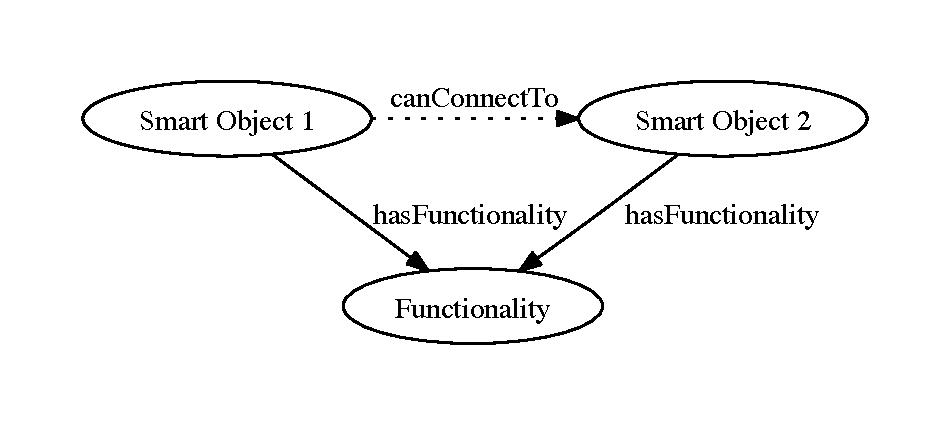
\includegraphics[width=\linewidth]{canConnectTo}
        \caption{Inferring connection possibilities based on functionality}
        \label{canConnectTo}
\end{figure}

To prevent a smart object from having a \texttt{canConnectTo} relationship to itself (which will be the case for semantic transformers), the relationship is defined to be irreflexive. Inferring indirect connection possibilities is also possible with a property chain:\\

\noindent
canConnectTo~\ensuremath{\circ}~canConnectTo~\ensuremath{\sqsubseteq}~canIndirectlyConnectTo

%When the \texttt{connectedTo} relationship is inserted, we also want to infer a \texttt{indirectlyConnectedTo} relationship. It turns out that this is something that is not expressible in OWL. (Q2336 (02/02/2012))


\subsection{Representing functionalities as predicates}
\label{predicateFunctionality}
If we want to model the common functionalities between two smart objects, we can use the n-ary ontology design pattern \cite{Noy2006}.\marginpar{Ontology design patterns are discussed in Chapter \ref{OntologyEngineering}.} Unfortunately, this is not intuitively readable from its ontological representation, as shown in the top half of Figure \ref{naryFunctionality}. The representation looks complicated and is difficult to read. On the other hand, we can also directly infer the matched functionalities as predicates, instead of using n-ary representations. The result can be represented using three triples instead of nine triples, and it is also more intuitively understandable, as shown in the bottom half of Figure \ref{naryFunctionality}.

\begin{figure}[bth]\centerline{
        %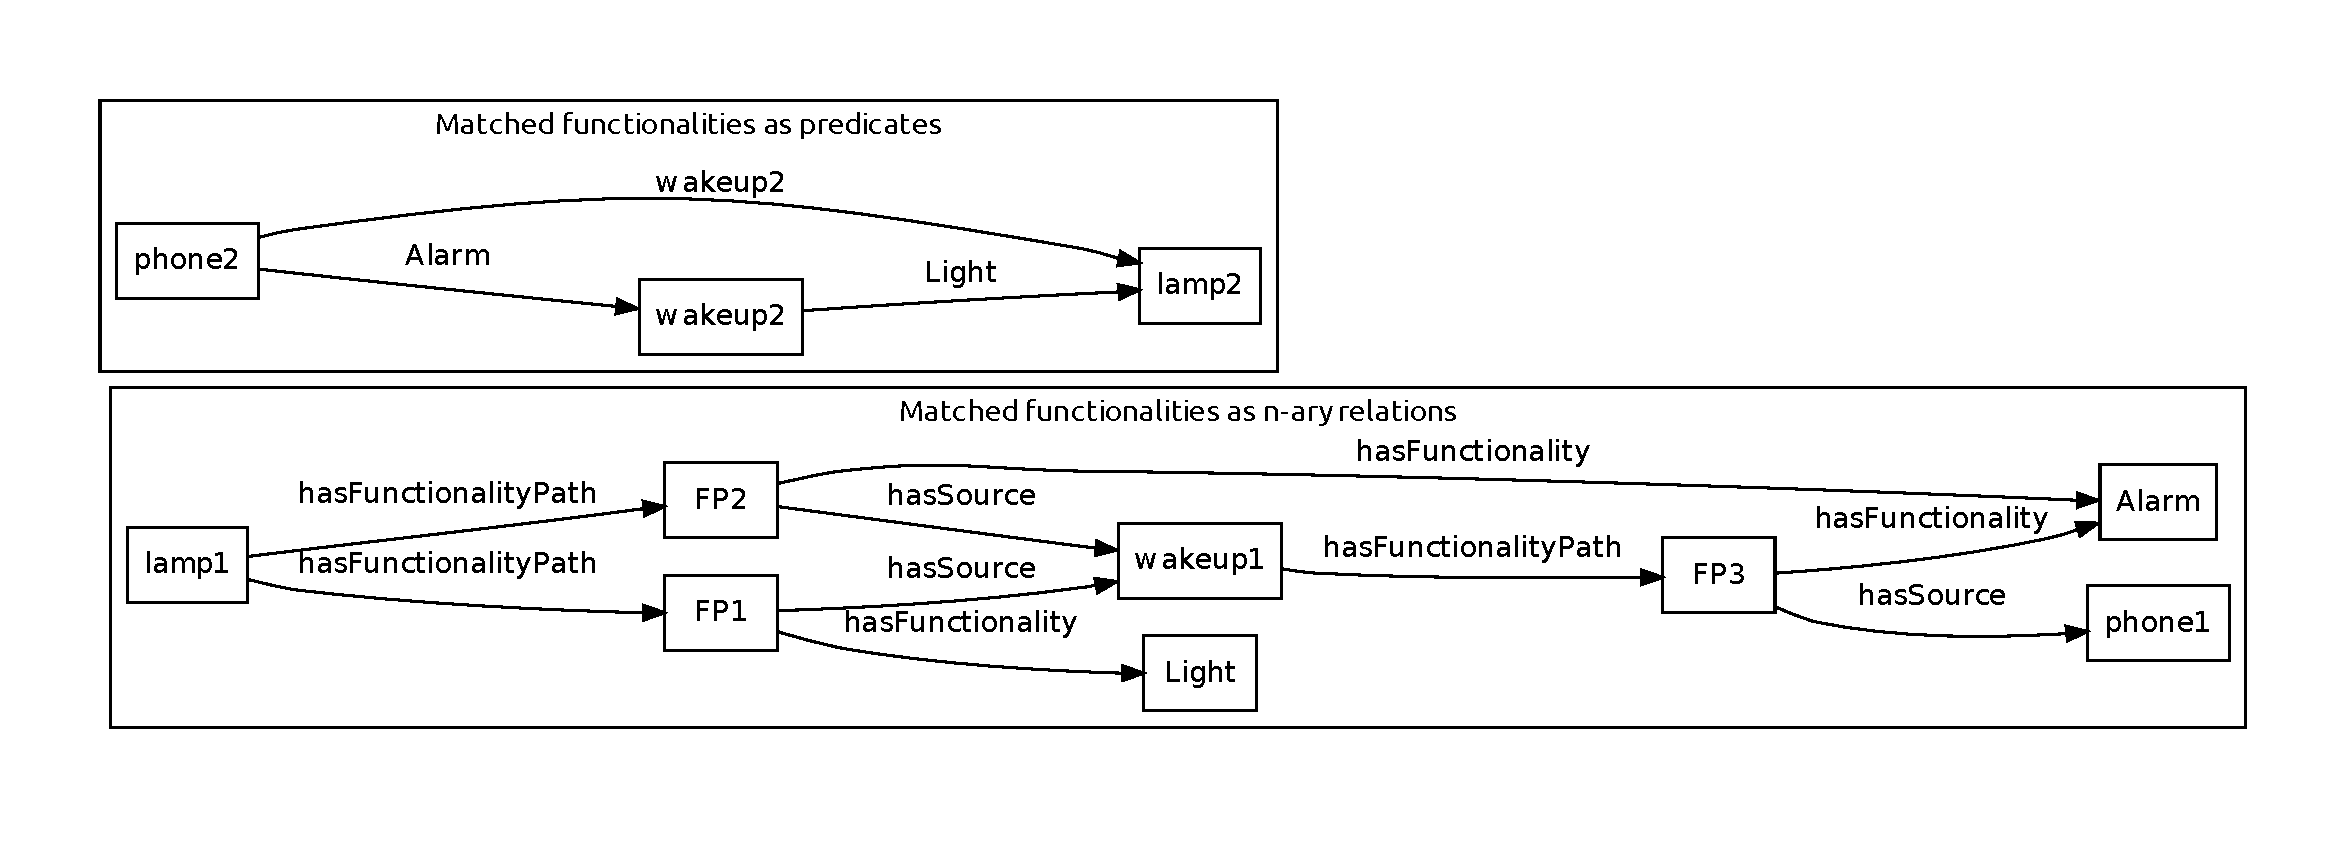
\includegraphics[width=450px]{naryFunctionality}
	\digraph[scale=0.45]{g}{
		rankdir=LR;
		compound=true;
		%fontname="Ubuntu";
		node [shape = box];
		lamp1->phone2 [style=invis]; % to ensure cluster0 is first
		subgraph cluster0 {
		label = "Matched functionalities as n-ary relations";
		lamp1 -> FP1 [label="hasFunctionalityPath"];
		FP1 -> Light [label="hasFunctionality"];
		FP1 -> wakeup1 [label="hasSource"];
		lamp1 -> FP2 [label="hasFunctionalityPath"];
		FP2 -> Alarm [label="hasFunctionality"];
		FP2 -> wakeup1 [label="hasSource"];
		wakeup1 -> FP3 [label="hasFunctionalityPath"];
		FP3 -> Alarm [label="hasFunctionality"];
		FP3 -> phone1 [label="hasSource"];
		}
		subgraph cluster1 {
		label = "Matched functionalities as predicates";
		phone2 -> wakeup2 [label="Alarm"];
		wakeup2 -> lamp2 [label="Light"];
		phone2 -> lamp2 [label="wakeup2"];
		}
	}
	}	
        \caption{Representing matched functionalities: N-ary relations versus predicates}
        \label{naryFunctionality}
\end{figure}

Representing an individual as a predicate is not valid in OWL 2 DL and places the ontology into OWL 2 Full. However, since we are using an OWL 2 RL/RDF Rules reasoning mechanism, this is not an issue. Thus we choose to use predicates instead of n-ary relations, and so we do not stay within OWL 2 DL. We can easily infer this relation using a \ac{SPIN} rule:

\begin{minted}{sparql}
CONSTRUCT {
    ?this ?functionality ?sink .
}
WHERE {
    ?this :functionalitySource ?functionality .
    ?sink :functionalitySink ?functionality .
}
\end{minted}

where \texttt{?this \ensuremath{\equiv} SmartObject}. For example, if we have a phone and a speaker with a common \texttt{Music} functionality, defined as

\begin{minted}{turtle}
:phone1 :functionalitySource :Music .
:speaker1 :functionalitySink :Music .
\end{minted}

the above \ac{SPIN} rule will infer

\begin{minted}{turtle}
	:phone1 :Music :speaker1 .
\end{minted}

such that the functionality itself is represented as a predicate. For a semantic transformer, which is indirectly connected to smart objects, we need an additional \ac{SPIN} rule:

\begin{minted}{sparql}
CONSTRUCT {
    ?source ?this ?sink .
}
WHERE {
    ?source :canIndirectlyConnectTo ?this .
    ?this :canIndirectlyConnectTo ?sink .
}
\end{minted}

where \texttt{?this \ensuremath{\equiv} SemanticTransformer}. This infers the semantic transformer itself as the relation between the source and the sink, since it transforms the original functionalities. For example, using the smart objects in Figure \ref{naryFunctionality}, if we have 

\begin{minted}{turtle}
	:phone2 :functionalitySource :Alarm .
	:wakeup2 :functionalitySink :Alarm .
	:wakeup2 :functionalitySource :Light .
	:lamp2 :functionalitySink :Light .
\end{minted}

and using the two property chains from Section \ref{ReasoningCapabilities}, we can infer that

\begin{minted}{turtle}
	:phone2 :canConnectTo :wakeup2 .
	:wakeup2 :canConnectTo :lamp2 .
	:phone2 :canIndirectlyConnectTo lamp2 .
\end{minted}

If we then apply the \ac{SPIN} rule defined above we can infer that 

\begin{minted}{turtle}
	:phone2 :wakeup2 :lamp2 .
\end{minted}

where the semantic transformer itself becomes the predicate between the two smart objects, signifying the possibility of having wakeup service functionality between the two objects.


How can we provide feedback or feedforward to the user that these possible functionalities exist between smart objects? This can be done using the feedback capability of the Connector object and the feedback capabilities of the devices themselves. Just after the user scans the second device, and before the connection is actually made, feedback of the different possibilities for shared functionality can be provided to the user. 

\marginpar{The \texttt{dataValue} property of interaction events is discussed in more detail in Section \ref{InteractionEvents}.} 
When two devices can be connected directly, the Connector object creates a temporary connection from itself to the sink. This temporary connection is specified using the \texttt{tempConnectedTo} property, a sub-property of the \texttt{connectedTo} property. The Connector object generates a \texttt{PreviewEvent} with the matching functionality as \texttt{dataValue}. This triggers the sink to create a preview of the functionality described by the \texttt{PreviewEvent} and its \texttt{dataValue}.  When the sink completes the preview, it generates its own \texttt{PreviewEvent} to indicate that it has finished. The Connector object sees the sink's \texttt{PreviewEvent} and removes the temporary connection.\marginpar{Preview events and the \texttt{tempConnectedTo} property were first discussed in Section \ref{section:augmentedFunctionalFf}.} 

\begin{figure}[bth]
	\digraph[scale=0.6]{stPreview}{
		{rank=same; Source; ST [label="Semantic Transformer"]; Sink;}
		{rank=max; Connector}
		Connector->ST [label= "tempConnectedTo"];
		ST->Sink [label = "tempConnectedTo"];
		Source->ST [label = "canConnectTo", style="dotted"];
		ST->Sink [label = "canConnectTo", style="dotted"];
		Source->Sink [label = "canIndirectlyConnectTo", style="dotted"];
	}
	\caption{Temporary connections for \texttt{PreviewEvent} when semantic transformer is used}
	\label{stPreview}        
\end{figure}

However, when there is a semantic transformer between the source and the sink, the Connector object creates a temporary connection to the semantic transformer instead of the sink, in order to generate the appropriate \texttt{PreviewEvent}, as shown in Figure \ref{stPreview}. Keep in mind that the semantic transformer is a virtual object, and therefore only the preview functionality generated by the sink will be perceivable by the user.

The Connector object uses the inferred \texttt{canIndirectlyConnectTo} and \texttt{canConnectTo} properties to determine where to insert the \texttt{temp\-Connected\-To} properties. After inserting the \texttt{tempConnectedTo} properties, the Connector object generates a \texttt{PreviewEvent}. Due to the \texttt{tempConnectedTo} relationship between the Connector object and the semantic transformer, the semantic transformer responds to this event and also generates a \texttt{PreviewEvent} with its own functionality as \texttt{data\-Value}. Due to the \texttt{tempConnectedTo} relationship between the semantic transformer and the sink, the sink responds to the preview event of the semantic transformer and generates the appropriate preview of its functionality.

Now that we have a way to model the capabilities of devices and provide previews of their functionality, we can start looking at ways to represent the different kinds of events that are generated on these devices in the next chapter.
\chapter{Event modelling}
\label{EventModelling}

\begin{flushright}{\slshape    
[Artefacts] mediate activity that connects a person not only with \\
 the world of objects, but also with other people. This means \\
that a person's activity assimilates the experience of humanity.} \\ \medskip
    ---  Aleksei N. Leontiev, founder of activity theory
\end{flushright}

\marginpar{Parts of this chapter appear in \cite{Niezen2011}.}

Events are notable occurrences that can be associated with people, places and objects at a specific time instant, or during a specific time interval. In the previous chapter the modelling of objects and their capabilities was described. The focus of this chapter is on how the event and its associated time instant/interval can be modelled. The modelling of people and places is considered to be outside the scope of this thesis.

%- Event ontology
%- Music ontology (uses Events ontology, also see 15/02/11)

\marginpar{Interaction events were first introduced in Section \ref{OntologyDesign1}.}
Interaction events are generated when a user interacts with a smart object. Interaction events are high-level input events which report the intention of the user's action directly, rather than just reporting the associated hardware input event that triggered the action. This high level of abstraction enables developers to write applications which will work across different devices and services, without having to write specific code for each possible input device. 

The W3C Web Events Working Group defined four conceptual layers for interactions, in the context of touch- and pen-tablet interaction \cite{w3cevents}:

\begin{description}
\item [Physical] This is the lowest layer, and deals with the physical actions that a user takes when interacting with a device, such as pressing a physical button.
\item [Gestural] This is layer describes mappings between the lower and upper layers; for example, a ``pinch'' gesture may represent the user placing two fingers on a screen and moving them together at the physical layer. This may map to a ``zoom-in'' event at the representational layer.
\item [Representational] This layer indicates the means by which the user is performing a task, such as zooming in, panning, navigating to the next page, activating a control, etc.
\item [Intentional] This layer indicates the intention of the task a user is trying to perform, such as viewing more or less detail (zooming in and out), viewing another part of the larger picture (panning), and so forth.
\end{description}

Interaction events can be defined at three of the layers, with the exception of the intentional layer. In Table \ref{transformationTable} examples of possible interaction events are shown, together with possible entities associated with these events. Most of these interaction events exist at the representational layer, which are events that have significant meaning.

\begin{table}
\centering
\begin{tabular}{|l|l|}
\hline
Interaction Event & Entity this event can be performed on\\
\hline
AdjustLevelEvent & Volume, Lighting \\
switchOnEvent & Lighting, any SmartObject \\
NavigateEvent & Playlist, Menu, SequentialData \\
UndoEvent & Any other interaction event \\
StopEvent & Application, Media \\
%DragAndDrop & Media \\
%Query & Media, other events \\
\hline
\end{tabular}
\caption{Examples of interaction events in a smart environment}
\label{transformationTable}
\end{table}



%An interaction event has more than one possible entity that it can be performed on, as well as more than one possible entity that triggers it, i.e., there exists some ambiguity. Only when no ambiguity exists as to which entity it is performed on, as well as the action which the user is trying to accomplish, we refer to it as an intentional event. Semantic transformations occur between physical actions (such as pressing a button or doing a gesture) and representational events, as well as between representational events and intentional events.


%end S3E


These events all occur at a specific time or during a specific time interval. In \ac{OWL}, there are are two approaches to modelling time:

\begin{itemize}
	\item Using datatype properties -- event instances can be related to a literal with a \ac{XSD} datatype such as \texttt{xsd:date} or \texttt{xsd:dateTime}. %This is the approach that we used and is described later in this chapter.
	\item Using object properties -- classes are used to define temporal intervals, and event instances are linked to instances of these classes using object properties.
\end{itemize}

The advantage of linking event instances directly with dates is simplicity. There are fewer abstractions to deal with, and it is easier to sort events chronologically and compare them \cite{Shaw2009}. On the other hand, working with temporal intervals provide more flexibility and allows for more detailed temporal reasoning.

\section{Related work}
We now look at various existing event ontologies that we build upon to model interaction events in ubiquitous computing environments. We will also look at how temporal reasoning is performed with ontologies.

\subsection{The Event Ontology}
The \ac{EO}\footnote{http://motools.sf.net/event/event.html} was developed within the context of the Music ontology\footnote{http://purl.org/ontology/mo/} at Queen Mary, University of London. Although originally created to describe musical performances and events, it is currently the most commonly used event ontology in the Linked Data community \cite{Shaw2009}.

The Timeline\footnote{http://motools.sf.net/timeline/timeline.html} ontology, used to define time instants and intervals, also forms part of this collection of ontologies. Reasoning with temporal information is discussed further in Section \ref{TemporalReasoning}.  

\subsection{DUL}

The \ac{DUL} upper ontology is a lightweight version of the \ac{DOLCE} ontology. \ac{DUL} defines the class \texttt{Event} next to the disjoint upper classes \texttt{Object}, \texttt{Abstract} and \texttt{Quality} \cite{Scherp2011}. \ac{DUL} allows for both the approaches to modelling time with \ac{OWL}, either with the \texttt{hasEventDate} datatype property, or with a \texttt{TimeInterval} class and the \texttt{isObservableAt} object property.

Events can be related to a \texttt{Place} with the \texttt{hasLocation} property. Alternatively, events can be related to a \texttt{SpaceRegion} with the \texttt{hasRegion} property, where \texttt{Space\-Region} resolves to a geospatial coordinate system. \ac{DUL} uses a \texttt{hasParticipant} property to relate an event to an object, and uses the \texttt{hasPart} property to link events to sub-events.

\subsection{Event-Model-F}

The Event-Model-F ontology extends the \ac{DUL} ontology to describe events in more detail. To describe the participation of an object in an event, the Event-Model-F ontology uses the \ac{DnS} ontology design pattern \cite{Shaw2009}.\marginpar{The \ac{DnS} pattern is described in more detail in Chapter \ref{OntologyEngineering}.} 

An object is defined as a \texttt{Participant}, where \texttt{LocationParameter} is used to describe the general spatial region of the object \cite{Scherp2011}. \texttt{Time\-Parameter} describes the general temporal region when the event happened by parametrizing a \ac{DUL} \texttt{TimeInterval}. A composite event \texttt{Composite} is composed out of a number of \texttt{Component}s.

\subsection{Linked Open Descriptions of Events (LODE)}

The \ac{LODE} ontology\footnote{http://linkedevents.org/ontology/} is an ontology for publishing descriptions of historical events as Linked Data. It builds upon the work of the previous ontologies described in this section, in order to improve interoperability with legacy event collections. Its \texttt{Event} class is directly equivalent to those defined by \ac{EO} and \ac{DUL}. 

It uses time intervals to link events to ranges of time, where its \texttt{atTime} property is a sub-property of the \ac{DUL} \texttt{isObservableAt} property. There is also a distinction between places and spaces, where the \texttt{inSpace} property relates the event to a space, and the \texttt{atPlace} property is a sub-property of the \ac{DUL} \texttt{hasLocation} property.


\subsection{Ontologies for temporal reasoning}
\label{TemporalReasoning}

Temporal reasoning is used when working with time intervals, for example when using Allen's Interval Algebra to define temporal relations between events. There are 13 base relations in this algebra, for example to define that event X happens before event Y, or that event X occurs during event Y. Allen's Interval Algebra is used by a number of ontologies, including the \ac{DOLCE} \cite{Scherp2011} upper ontology. \marginpar{The \ac{DOLCE} upper ontology is discussed in more detail in Chapter \ref{OntologyEngineering}.}

\ac{SWRL} Basic Temporal Built-ins support \texttt{xsd:date} and \texttt{xsd:dateTime} with Allen's Interval Algebra. The Advanced Temporal Built-ins uses the \texttt{temporal} ontology \cite{OConnor2010} to provide additional functionality, for example having different granularity levels.


The \ac{DC} Terms ontology has a \texttt{temporal} property to describe temporal coverage of a resource with a range \texttt{periodOfTime}.

TopBraid Composer has a Calendar ontology that defines an \texttt{Event} and its \texttt{startTime} and \texttt{endTime} (as \texttt{xsd:dateTime}). This can then be used with the Calendar View widget in the editor. 

In \ac{SPARQL}, we can use the $<$ and $>$ operators on dates, for example 

\begin{verbatim}
FILTER(?date > "2005-10-20T15:31:30"^^xsd:dateTime)
\end{verbatim}

Using \ac{SPIN}, can also cast a \texttt{xsd:dateTime} value to a string using the \texttt{fn:substring} function, for example

\begin{verbatim}
fn:substring(xsd:string(afn:now()),0,10)
\end{verbatim}


\section{Interaction events}
We now turn our focus to how interaction events are modelled in the work described in this thesis. An interaction event happens at a specific time, is generated by a smart object and has an optional data value associated with the event.

\begin{figure}[bth]
        \includegraphics[width=\linewidth]{interactionEvent}
        \caption{An interaction event as modelled in the ontology}
        \label{interactionEvent}
\end{figure}

An example of an event generated when an alarm is set is
\begin{minted}{turtle}
:event-43495d51-29e3-11b2-807e-ac78eefc1f82 
	rdf:type :AlarmSetEvent ;
	:generatedBy :phone1 ;
	:inXSDDateTime "2012-01-17T11:22:06.887+01:00"^^xsd:dateTime ;
	:dataValue "2012-01-17T12:00:00+01:00"^^xsd:dateTime .
\end{minted}

A mapping between our interaction event model and the other event ontologies is shown in Table \ref{eventMappings}. Note that we do not model people or places in the current version of the ontology, as we consider these entities to be optional when describing interaction events.

\begin{table}
    \myfloatalign
  \begin{tabularx}{\textwidth}{llll} 
	\toprule
    \tableheadline{DUL} & \tableheadline{EO} & \tableheadline{LODE} & \tableheadline{Interaction Events}\\ 
    \midrule

isObservableAt & time & atTime & inXSDDateTime  \\
 & place & inSpace & \\
hasLocation & & atPlace & \\
hasParticipant & factor & involved & \\
involvesAgent & agent & involvedAgent & generatedBy \\
& & & dataValue \\	
    \bottomrule
  \end{tabularx}
  \caption{Mappings between the various event models (adapted from \cite{Shaw2009})}\label{eventMappings}
\end{table}



The \texttt{duration} property is used to define the length of event. For example to increase the brightness of a lamp, we can generate an event to increase a value to a set maximum over a time period:

\begin{minted}{turtle}
:event-43495d51-29e3-11b2-807e-ac78eefc1f83 
	rdf:type :IncreaseLevelEvent ;
	:generatedBy ie:wakeup1 ;
	:inXSDDateTime "2012-01-17T11:23:06.887+01:00"^^xsd:dateTime ;
	:dataValue 255 ;
	:duration "PT3S"^^xsd:duration .
\end{minted}


We also distinguish between \emph{control} and \emph{content}. Interacting with a device, e.g. pressing a ``Play'' button or moving a volume slider, is considered control and described using interaction events. Content, e.g. a song or a photo stored on the device,  is referred to by where it exists on the device, as well as how it can be rendered using the media capabilities of the device. 

We consider interaction events to be traceable, reversible and identifiable. Each interaction event has an associated timestamp and a unique ID that is generated when the event occurs. 

\marginpar{Intentional, incidental and expected interactions were introduced in Section \ref{intentionalSpectrum}.}
An intentional interaction, like pressing a light switch, is an interaction event if the light switch shares this information with other devices. Incidental or expected interactions, like the light turning on if the presence sensor is triggered, are also interaction events. System events, like a \texttt{TimeSetEvent}, which are invisible to the user are not considered to be interaction events.

\section{Categorising interaction events}

In the iStuff toolkit \cite{Ballagas2003} \emph{hierarchical event} structures were used to abstract low-level events into application-level events. \marginpar{Also see the related work on task models in Section \ref{interactionTasks}.} We also introduce the notion of an event hierarchy, where low-level events are considered to be very \emph{generic}, as they do not report a user's intention directly \cite{Niezen2011}. These low-level events first need to be transformed into intentional events---events that express user intention.

%some of this might need to move to, or be repeated in the section where we describe our interaction model.
%\marginpar{Nielsen's virtual protocol model and its interaction levels were discussed in Section \ref{nielsenVPM}.}
We build on the different interaction layers introduced in the related work of Section \ref{InteractionModels} to categorise interaction events. As an example, consider the case where a rocker switch, modelled as an interaction primitive on a mobile device, is used to control the volume of music in a room. One could start modelling the interaction on the physical level with a \texttt{ButtonEvent}, but it would be more meaningful to model it on the lexical level as a \texttt{ButtonUpEvent}. On the syntactic level this event could increment a quantity by one, while an event generated by a volume dial might have a discrete value attached to it. When this is combined with other device information, for example that the device is being used to stream music to the environment, we can infer on the semantic level that it is a \texttt{VolumeUpEvent}. When this is combined with other contextual information, for example that the device is currently connected to a speaker system in the same room, we can even infer on the task level that the music volume in the room should be set to a specific value with a \texttt{MusicVolumeUpEvent}, to which all connected devices can respond. We acknowledge that in most cases it may not be possible to make inferences on the goal level, which in this example could be the user's intent to set the music volume in the room to a level that is loud enough for everyone in the room to dance to.

\begin{figure}[bth]
	\digraph[scale=0.45]{InteractionModelToOntology}{
		{rank=same; Semantic [label="Semantic Level", shape=plaintext]; AdjustLevelEvent; MusicVolumeUpEvent }
		{rank=same; Syntactic [label="Syntactic Level", shape=plaintext]; VolumeUpEvent; SmartObject;}
		{rank=same; Lexical [label="Lexical Level", shape=plaintext]; ButtonUpEvent}
		{rank=same; Alphabetic [label="Alphabetic Level", shape=plaintext]; ButtonEvent; }
		Semantic->Syntactic->Lexical->Alphabetic [style="invis"];
		ButtonEvent->ButtonUpEvent;
		ButtonUpEvent->VolumeUpEvent
		VolumeUpEvent -> MusicVolumeUpEvent;
		MusicVolumeUpEvent -> AdjustLevelEvent  [label="is-a"];
		VolumeUpEvent -> SmartObject [label="generatedBy"];
		AdjustLevelEvent -> SmartObject [label="generatedBy", style="dashed"];
	}
	\caption{How the interaction model levels relate to the ontology}
	\label{InteractionModelToOntology}        
\end{figure}

Figure \ref{InteractionModelToOntology} shows how the interaction model levels relate to the concepts in the ontology that was developed through the various iterations. A \texttt{ButtonEvent} describes a user interaction on the alphabetical level, but carries very little meaning. For example, was the button switched up or down, or was it pressed? If we know that the button was switched up, we have a lexical token that describes the interaction, but it still needs to be combined with other contextual information to determine the user's intention. On the other hand, if the interaction is described as a \texttt{VolumeEvent}, the user's intention is described on a syntactic level, and it becomes possible to map the event to a set of predefined semantic events, for example an \texttt{AdjustLevelEvent}. Using semantic reasoning, we can also infer that this \texttt{AdjustLevelEvent} was generated by the same smart object.




\subsection{System events}
\label{SystemEvents}
When a smart object first subscribes to the smart space, it specifically listens for events that are generated by other smart objects connected to it. This means that we also need some way of distributing system-wide events that all devices listen for. As an example, consider the \texttt{TimeSetEvent}. When the user sets the time on one device, we want the time to be immediately updated on all the other smart objects in the smart space, even if they are not connected to the device that generated the \texttt{TimeSetEvent}. If we define \texttt{TimeSetEvents} as a subset of \texttt{SystemEvents}, each smart object only need to subscribe to events of type \texttt{SystemEvent}.


\subsection{Feedback}
When setting an alarm for example, augmented feedback should be provided on all devices. Functional feedback, i.e. the alarm sound when an alarm fires is triggered, is delayed. This means that augment functional feedforward should be provided. We thus define two types of feedback events:\marginpar{Preview events and indicator events were first introduced in Section \ref{section:augmentedFunctionalFf}.}

\begin{itemize}
\item \texttt{PreviewEvent} - generated when a possible connection is being explored, displaying the possible functionalities enabled by the connection, i.e. augmented functional feedforward.
\item \texttt{IndicatorEvent} - augmented feedback when smart object is connected and there is no immediate functional feedback, e.g. a sink ``beeping'' when the alarm is set on the source; used to confirm actions.   
\end{itemize} 

The type of feedback required depends on the functionality of the connection. It is important for the feedback to coincide in time and modality with the event generated, as to maintain the causal link that is perceived by the user.

The device used to make the connection, for example the Connector object, creates a temporary connection to the devices to be connected in order to generate a \texttt{PreviewEvent}. This \texttt{tempConnectedTo} property is a sub-property of the \texttt{connectedTo} property. This means that the smart objects will handle it as if it is a regular connection, and when the Connector object removes the \texttt{tempConnectedTo} relationship, the inferred \texttt{connectedTo} relationship will disappear as well.


\subsection{Discussion \& Conclusion}

Tungare et al. \cite{Tungare2007} defined a \emph{task disconnect} as ``the break in continuity that occurs due to the extra actions outside the task at hand that are necessary when a user attempts to accomplish a task using more than one device.'' Kuniavsky \cite{Kuniavsky} states that consistency is the key aspect in creating task continuity across devices, and that \emph{interaction vocabularies} have recently emerged as a way of consistently interacting with a range of devices. This ranges from simple vocabularies of light patterns and motion as used by the (now discontinued) Nabaztag Internet-connected rabbit that could compose ``sentences'' with more complex meaning, to a set of visual icons by Timo Arnall \cite{Arnall2006} that represents various kinds of touch-based RFID interactions. Arnall's touch-based vocabulary is shown in Figure \ref{arnall}. Arnall categorises his vocabulary of visual icons into four classes of interactions: 

\begin{itemize}
	\item Circles, of which the ``Aura'' is an example
	\item Card, of which the ``Card in hand'' is an example
	\item Wireless, of which the ``Wireless dot'' is an example
	\item Mobile, of which the ``Phone beaming'' is an example
\end{itemize}

\begin{figure}[bth]
	\begin{center}
        \includegraphics[width=250px]{arnall}
	\end{center}
        \caption{Examples from Arnall's ``A graphic language for touch'' (adapted from \cite{Arnall2006})}
        \label{arnall}
\end{figure}

The ``Aura'' icon communicates both the near-field communication capabilities of the technology, but also indicates that the physical object has capabilities beyond its form. The icons with cards or mobiles could improve consistency for a wide range of users which use these technologies on a daily basis.

These interaction vocabularies try to smooth over task disconnects through consistency. We argue that by having a vocabulary, or ontology, for interaction events could improve consistency in ubiquitous computing environments. This is the intention of the work in this chapter --- to provide an ontology of interaction events that improves consistency for users, as well interoperability between devices.





% TODO: Valkkynen2010,  Rekimoto et al. (Ayatsuka2003), Nordby2010

% http://www.elasticspace.com/presentations/graphic_language_touch_rfid_nfc.pdf

% Possible TODO: How we developed a vocabulary for semantic connections

% Possible TODO: Creating a vocabulary of interaction events (based on existing task models)



% ===Event modelling
% To model an \texttt{AlarmSetEvent}, the following restriction was used:\\
% 
% \noindent
% \texttt{AlarmSetEvent}~$\models$~\texttt{SetEvent}~$\sqcap$~\texttt{dataValue}~$\forall$~\texttt{xsd:dateTime}~$\sqcap$~\texttt{dataValue}~$= 1$\\
% 
% This restriction will not infer that an event is an \texttt{AlarmSetEvent}, but it will restrict the descriptions of these events to what can actually be described.

\chapter{OntologyEngineering}
\label{OntologyEngineering}


How can we model an ontology for smart environments that allows developers to specify a smaller amount of information, and then use semantic reasoning to derive the remainder automatically?

In SOFIA, a reasoner may also be used for truth maintenance, belief revision, information consistency and/or information creation \cite{Oliver2008}.


When applying inference to the physical world, the level of ambiguity and uncertainty is quite high. A system might infer that you are in a room because your RFID badge is in a room. What if you forgot your badge in the office? The challenge is to figure figure out what functions in the smart home are possible with limited inference, which are possible only through inference, and which require an oracle \cite{Edwards2001}. Systems that rely on inference will be wrong some of the time, and users will need to have models to figure out how the system arrives at its conclusions, along with ways to override the system's behaviour.


The CanBe pattern: infers new object property between entities when certain conditions have been fulfilled, e.g. CanBeTransformedTo, canBeConnectedTo
To specify an object property as a union of two existing properties, we first need to define a new class that specifies the union, and then specify the object property as part of that class. This is necessary as a property cannot by itself be specified as a union of other properties.

the isClass pattern: Using local reflexivity (i.e. ObjectHasSelf) allows us to define a property that relates a class to itself. This can be used to transform a class to a property when creating property chains.
E.g.:
InputDevice is a Class.
InputDevice is defined as InputDevice some Self [Hoekstra, Social Reality]
chainProperty as property Chain: isInputDevice o someProperty o isInputDevice
This would allow the chainProperty to be inferred only between InputDevices that has the someProperty.
Can be used to prevent an inconsistent ontology by only allowing certain domains and ranges to be inferred.

connection properties: using property chains to identify a path of interconnected properties

Pattern: Using pre-defined individuals to define a range of values/cases, since instances of classes can only be related to other individuals.



Dodds and Davis \cite{Dodds2011} used the following structure to document an ontology design pattern in their book ``Linked Data Patterns'':

\begin{itemize}
	\item Question - A question indicating the problem the pattern is designed to solve
	\item Context - Description of of the goal and context of the pattern
	\item Solution - Description of the pattern
	\item Example(s) - Real-world implementations that make use of this pattern
	\item Discussion - Analysis of the pattern and where it can be used
	\item Related - List of comparable patterns
\end{itemize}



\section{Naming interaction events}

\emph{How should the \ac{URI} of an interaction event be structured so that the name forms a natural hierarchy?}

\subsection{Context}

Interaction events tend to form natural groups, such as events related to a specific device class. Reflecting these groups in the name of the interaction event itself makes it easier for developers to understand existing and/or inferred groupings, and to classify new events into an existing hierarchical event structure.

\subsection{Solution}

We use the notation\\ 

\noindent
\texttt{[DeviceClass][Action]Event}\\

 to define the interaction event. 

\subsection{Example(s)}

Consider a simple light switch with two states, \texttt{Up} and \texttt{Down}. We can define two interaction events, \texttt{switchDownEvent} and \texttt{switchUpEvent}, which can then later be grouped by either device class or by action.

\subsection{Discussion}

If the naming convention of a \ac{URI} follows a common pattern, they become easier to remember and easier to work with. They can even be constructed automatically. It makes the \ac{URI} human-readable and improves the relation between the name and the event it describes. 

\subsection{Related}

\begin{itemize}
	\item Hierarchical URIs \cite{Dodds2011}
	\item Patterned URIs \cite{Dodds2011}
\end{itemize}




\section{Qualified Cardinality Restrictions}

In \ac{OWL} 2, it is possible to define a \ac{QCR}, which means the cardinality restriction can be applied to a specific class \cite{Hebeler2009}. In \ac{OWL} 1, defining something like  


 This means that it is possible to define that a smart object has only one current state:

\begin{minted}{turtle}
	SmartObject
	rdfs:subClassOf
	          [
	            rdf:type owl:Restriction;
	            owl:qualifiedCardinality 1;
	            owl:onProperty hasCurrentState;
	            owl:onClass State
	          ];
\end{minted}

If we then assert a certain smart object to have two current states, e.g.

\begin{minted}{turtle}
	phone1 hasCurrentState playing .
	phone1 hasCurrentState stopped .
\end{minted}

it will violate the QCR if \texttt{playing} and \texttt{stopped} are distinct\footnote{Asserted that they are different individuals}. In earlier versions of OWL, it was not possible to define a specific class for a cardinality restriction. 



\subsection{Semantic transformers}
In the sleep use-case, a semantic transformer was implemented in order to generate lighting values for the dimmable lamp to create the desired wakeup experience. During the implementation, several observations and decisions were made:

\begin{itemize}
\item 	Between smart objects and semantic transformers only \texttt{indirectlyConnectedTo} connections can exist, as the semantic transformers are virtual entities that cannot be directly connected to smart objects using the Connector object.
\item 	When a \texttt{canIndirectlyConnectTo} relationship is inferred between smart object A and the semantic transformer B, and between B and smart object C, a \texttt{canConnectTo} relation between A and C should be inferred (transitive).
\item 	When a connection is made between two smart objects that can be connected through a semantic transformer, the semantic transformer is connected to the smart objects with  \texttt{indirectlyConnectedTo} relationships, and a \texttt{connectedTo} relationship between the smart objects is then automatically inferred.
\item 	A semantic transformer thus acts as a bridge.
\item 	A semantic transformer is \emph{not} a smart object. 
\end{itemize}

%\subsubsection{Using semantic transformers for control}
When using semantic transformers to control other smart objects, we could make use of the n-ary ontology design pattern, which was also applied to creating media paths in Section \ref{SemanticMatching} on semantic matching: %\marginpar{Ontology design patterns are discussed in more detail in Chapter \ref{OntologyEngineering}.}

\begin{itemize}
	\item Subscribe to \texttt{controlSource} to see if it becomes a control source
	\item When it becomes a control source, subscribe to the events generated by the control originator
\end{itemize}

While this is feasible, it is complicated and we would like to use a simpler solution using \texttt{connectedTo} relationships. What we would like to infer is shown in Figure \ref{semanticTransformerControl}.

\begin{figure}[bth] %no empty lines allowed
	\digraph[scale=0.6]{semanticTransformerControl}{
		node [shape=box];
		{rank=same; Source; ST [label="Semantic Transformer"]; Sink;}
		Source -> ST [label="canConnectTo"];
		ST -> Sink [label="canConnectTo"];
		Source -> Sink [label="connectedTo"];
		Source -> ST [label="connectedTo", style="dashed"];
		ST -> Sink [label="connectedTo", style="dashed"];
	}
	\caption{Inferring \texttt{connectedTo} relationships between sources/sinks and a semantic transformer}
	\label{semanticTransformerControl}        
\end{figure}

Basically, what we are trying to model could be called a ``property intersection'', where\\

\noindent
\texttt{x P1 y}~$\sqcap$~\texttt{x P2 y}~$\vdash$~\texttt{x P3 y}\\
%see Q2336 Preventing other individuals in a class from inferring the same property

At first glance, it seems like this might be expressed using property chains and local reflexivity, as described in the ontology design pattern in Section \ref{LocalReflexivity}. However, this is a special case which cannot be expressed in \ac{OWL}. It can, however, easily be expressed as a \ac{SPIN} rule as follows:

\begin{minted}{sparql}
CONSTRUCT {
    ?source :connectedTo ?semanticTransformer .
    ?semanticTransformer :connectedTo ?sink .
}
WHERE {
    ?source :canConnectTo ?semanticTransformer .
    ?semanticTransformer :canConnectTo ?sink .
    ?source :connectedTo ?sink .
}
\end{minted}







Possible TODO Pushing the boundaries, e.g. with SPIN
\label{SPIN}





\chapter{Software architecture}
\label{SoftwareArchitecture}

\begin{flushright}{\slshape    
Interaction is an iterative process of listening, thinking, \\
and speaking between two or more actors.} \\ \medskip
    --- Chris Crawford, game designer
\end{flushright}

\marginpar{Parts of this chapter have previously appeared in \cite{Niezen2010} and \cite{Niezen2012}}

Existing architectural patterns for software like the \ac{MVC} model, Document-View and Presentation-Abstract-Control are considered to be inadequate when trying to design software architectures in the ubiquitous computing domain. Ubiquitous computing needs new kinds of mechanisms to meet the flexibility needed to change the purpose, functionality, quality and context of a software system \cite{Niemela2004}.\marginpar{\ac{MVC} was first mentioned in Section \ref{uisa}.}

In this chapter the software architecture used in the three design iterations is described in more detail. It is quite a short chapter, as most of the software architecture issues have already been discussed in the three design iteration implementations in Sections \ref{D1Implementation}, \ref{D2Implementation} and \ref{D3Implementation}. However, we consider it important that the final software architecture design has its own dedicated chapter, so that it can act as a reference design for future implementations.

We first look at some characteristics of ubicomp middleware, followed by a discussion of the publish/subscribe paradigm and the blackboard architectural pattern. We then look at the \ac{MOM} implementation used with\-in the \ac{SOFIA} project, called \ac{SSAP}. The rest of the chapter is dedicated to the two main implementations of the software architecture as used within the \ac{SOFIA} project -- Smart-M3 and ADK-SIB. These implementations are interoperable with one another through the use of \ac{SSAP}.


\section{Characteristics of ubicomp middleware}

There are a number of characteristics, or quality attributes, that are specific to middleware for ubiquitous computing, as defined by Niemel\"a and Vaskivuo \cite{Niemela2004}:

\begin{itemize}
	\item Interoperability
	\item Scalability 
	\item Reusability
	\item Maintainability
	\item Extensibility
	\item Portability
	\item Adaptability
	\item Survivability
	\item Agility
	\item Fidelity
\end{itemize} 

Interoperability is defined as the ability for software applications written in different programming languages, running on different platforms with different operating systems, to communicate and interaction with one another over different networks. Scalability is the ability of the system to handle larger numbers of smart objects. Re\-us\-a\-bility, maintainability and extensibility are characteristics that consider the evolution of software systems. Portability and adaptability are important characteristics for software that has to work in a heterogenous system of devices and networks. Survivability is the ability of a system to timely deliver essential services in the face of attack, failure or accident. Agility is the sensitivity to changes in resource availability. Fidelity is defined to mean to degree to which data presented on a client matches the reference copy at the server.

We focused on a subset of these attributes while working on the software architecture, including interoperability, reusability, maintainability and extensibility. Interoperability was achieved by adhering to the \ac{SSAP} specification, as described in more detail in Section \ref{ssap}. Using ontologies and other Semantic web technologies helped us to improve reusability, while elements of maintainability were tested using the Cognitive Dimensions framework, described in more detail in Chapter \ref{Evaluation}. Extensibility was achieved by modelling devices and their capabilities in such a way that other devices could easily be added to the system.
\marginpar{Potential scalability was tested by evaluating the performance of the software architecture, as described in Section \ref{performance}.}
% \subsection{Context}
% 
% Context is information that can be used to characterise the situation of an entity, where an entity can be a person, place, or physical or computational object \cite{Gu2004}. Context awareness is the capability of ubiquitous computing middleware to handle unpredictable changes \cite{Niemela2004}. Application-aware adaption is part of context awareness, defined to mean to collaboration between the system infrastructure and the individual applications on the devices.


\section{Publish/subscribe paradigm and the blackboard architectural pattern}
\label{pubsubblackboard}
In publish/subscribe systems, subscribers register their interest in a specific event, and are notified when this event occurs after a publisher publishes the event. The strength of the publish/subscribe par\-a\-digm is that entities are decoupled in time, space and synchronisation \cite{Eugster2003}. Space decoupling means that the interacting entities do not need to be aware of each other. Time decoupling means that the entities do not need to participate in the interaction at the same time. Synchronisation decoupling means that subscribers can asynchronously be notified when an event occurs. Removing synchronisation dependencies between entities increases scalability.

There are three variants of publish/subscribe systems:

\begin{itemize}
	\item Topic-based -- Entities subscribe to individual topics, usually with some form of hierarchical addressing to organise the topics
	\item Content-based -- Consumers subscribe to selective events by specifying filters, using some kind of subscription language
	\item Type-based -- Events are filtered according to their type
\end{itemize}

In the \ac{SOFIA} project, \acp{KP} communicate with a message broker using the blackboard architectural pattern, where the message broker uses a triple store as a common knowledge base. Communication between \acp{KP} occurs through the insertion and removal of triples into or from the triple store.  Given a set of smart devices, the blackboard may be used to share information between these devices, rather than have the devices explicitly send messages to one another. If this information is also stored according to some ontological representation, it becomes possible to share information between devices that do not share the same representation model, and focus on the semantics of that information \cite{Oliver2008}. The \ac{SIB} is the information store of the smart space, and contains the blackboard, ontologies, reasoner and required service interfaces for the \acp{KP} or agents.

This blackboard approach is complemented by a publish/subscribe component, that allows \acp{KP} to subscribe to specific triples in the triple store. The \acp{KP} are then notified when these triples are added, removed or updated in the triple store. Communication between the \acp{KP} and \ac{SIB} occurs using \ac{SSAP}, which is the focus of the next section.

%Publish/Subscribe mechanism (http://en.wikipedia.org/wiki/Publish/subscribe , distributed event handling system, Observer pattern as a subset that can be compared with MVC pattern, see) vs polling mechanism


%SISS2010 start

%\section{Architectural patterns for pervasive computing}

%The approach used in \ac{SOFIA} is to make use of a blackboard architectural pattern to enable cross-domain interoperability. 



%SOFIA takes the agent, blackboard and publish/subscribe concepts and re-implements them in a lightweight manner suitable for small, mobile devices. These agents, which are termed \acp{KP} can operate autonomously and anonymously by sharing information through blackboard spaces (see Figure \ref{blackboard}). T

%SISS2010 end


\section{Smart Space Access Protocol (SSAP)}
\label{ssap}

\ac{MOM} is used to send messages between components in a distributed system. Commercial options include \ac{JMS}, \ac{MSMQ} and IBM's WebSphere framework.  \ac{AMQP} is an emerging standard, of which RabbitMQ\footnote{http://www.rabbitmq.com/} is a popular implementation. ZeroMQ\footnote{http://www.zeromq.org/}, also written as \O MQ , was created to be simpler and faster than the \ac{AMQP} standard, and does not require a dedicated message broker. Other message protocols include \ac{XMPP}, \ac{MQTT} and \ac{STOMP}.\marginpar{\ac{XMPP} is an \ac{IETF} standard.}

In the \ac{SOFIA} software architecture, \acp{KP} communicate with the \ac{SIB} through \ac{SSAP} messages \cite{Honkola2010} over TCP/IP. \ac{SSAP} consists of a number of operations to insert, update and subscribe to information in the \ac{SIB}. These operations are encoded using \ac{XML}.

For operations initiated by a \ac{KP}, the \ac{KP} sends a request message and the \ac{SIB} responds with a corresponding confirmation message. For \ac{SIB} initiated operations, the \ac{SIB} sends an indication message. The \ac{KP} does not respond to \ac{SIB} initiated operations, as indication messages contain non-essential information. Every session must start with a join operation, and a leave operation ends a session.

To insert information into the triple store, an insert operation is used by the \ac{KP}, where the triples are encoded in RDF/XML.  A \ac{SIB} confirmation message indicate whether the operation was successful or not. Similarly, a remove operation is used to remove information from the triple store. An update operation removes information from the triple store and inserts new information as an atomic operation.

To query the triple store, a template consisting of a list of triples is used, where each triple may have a wildcard as its subject, predicate or object. The result of the query is a list of all triples that match the template. All triples in the triple store that match any of the triples in the list are returned.

A subscribe operation creates a persistent query that is stored in the \ac{SIB} and is re-evaluated automatically after each change to the contents of the triple store. An unsubscribe operation will terminate a persistent query. The publish/subscribe mechanism used is closest in scope to the content-based variant described in the previous section.

\ac{SSAP} is supported by both the \ac{SIB} implementations used in our work, such that software developed for the one implementation is also interoperable with the other implementation. We now focus in more detail on these two implementations: Smart-M3 and ADK-SIB.\marginpar{The Smart-M3 implementation was used during the first design iteration, while the ADK-SIB implementation was used during the second and third design iteration.}


%SeNAmI start
\section{Smart-M3 architecture}
\label{m3}
The M3 (multi-device, multi-vendor, multi-domain) architecture is an interoperability platform based on a blackboard architectural model that implements the ideas of space-based computing \cite{Honkola2010}. It consists of two main components: a \ac{SIB} that acts as a common, semantic-oriented store of information and device capabilities, and \acp{KP}, virtual and physical smart objects that interact with one another through the \ac{SIB}. Various \ac{SIB} implementations exist that conform to the M3 specification of which Smart-M3, developed by Nokia, was the first open source reference implementation released in 2009\footnote{http://sourceforge.net/projects/smart-m3/}. \ac{RIBS}, developed by VTT, is a C-based implementation of M3 targeted for devices with low processing power, but requires a large amount of memory \cite{Etelapera2011}.  


\section{ADK-SIB}

The \ac{SIB} implementation used during the second and the third design iteration is called ADK-SIB (Application Development Kit SIB) and was developed within the \ac{SOFIA} project. The ADK-SIB is a Jena-based\footnote{http://jena.sourceforge.net/} \ac{SIB} written in Java and runs on the \ac{OSGi} framework.

Reasoning in the standard ADK-SIB is implemented using the Jena Ontology API, but only basic reasoning with symmetric properties and transitive properties is supported. Our main contribution to improve the ADK-SIB implementation was to implement support for OWL 2 RL/RDF Rules reasoning, as well as \ac{SPIN} rules using the TopBraid \ac{SPIN} API\footnote{http://topbraid.org/spin/api/}.\marginpar{The ADK-SIB and SPIN API was first mentioned in Section \ref{adk-sib}.}

When the \ac{SIB} starts up, we first load the ontology, written in \ac{OWL} 2, from a specified web address into our \emph{asserted} model. We then load the OWL 2 RL specification, specified as \ac{SPIN} rules, from another \ac{OWL} file. We also load any custom \ac{SPIN} functions into a third model. We then build a union model of the three models and store all the asserted triples in a hashmap to improve lookup efficiency. Finally the TopSPIN reasoning engine performs inferencing across the union model, and all the inferences are stored in the \emph{inferred} model.

Whenever a new triple is added, removed or updated, the inferred model is cleared and inferencing is performed using the reasoning engine. This means that no inferencing needs to be performed when a query is run. 

\begin{figure}[bth]
	\centering
	\centerline{\includegraphics[width=250px]{swarch}}
	\caption{Our software architecture}
	\label{swarch}
\end{figure}

The final software architecture is shown in Figure \ref{swarch}. The system performance of the software architecture was evaluated during the Smart Home pilot of the second design iteration, and this evaluation is described in the next chapter. A validation of the entire system, including the ontology, using the Cognitive Dimensions framework is also described.


% (the following was mentioned in DesignIteration2)
% With \ac{SPIN}, rules are expressed in \ac{SPARQL}, the W3C recommended \ac{RDF} query language, which allows for the creation of new individuals using CONSTRUCT queries. OWL (Web Ontology Language) inferences for the OWL 2 RL (OWL 2 Rule Language) profile were executed by using SPIN rules\footnote{ http://topbraid.org/spin/owlrl-all}. OWL 2 RL is a syntactic subset of OWL 2 that is amenable to implementation using rule-based technologies. According to the OWL 2 RL W3C page\footnote{http://www.w3.org/TR/owl2-profiles/\#OWL\_2\_RL} the OWL 2 RL profile is aimed at applications that require scalable reasoning without sacrificing too much expressive power.


%(\texttt{OWL\_DL\_MEM\_TRANS\_INF})

% A command-line tool called \texttt{ssls}\footnote{Available from \texttt{http://sourceforge.net/projects/ssls/}} was used to view information in the smart space.

%SeNAmI end

% The SOFIA IOP is based on a blackboard architectural model that implements the ideas of space-based computing \cite{Honkola2010}. It consists of two main components: a SIB (Semantic Information Broker) that acts as a common, semantic-oriented store of information and device capabilities, and KPs (Knowledge Processors), virtual and physical smart objects that interact with one another through the SIB. Various SIB implementations exist that conform to the M3 specification, of which Smart-M3 was the first open source reference implementation released in 2009\footnote{http://sourceforge.net/projects/smart-m3/}. RIBS (RDF Information Base System) is a C-based implementation of M3 targeted for devices with low processing power, but requires a high amount of memory \cite{Etelapera2011}.  The SIB implementation used in the pilot is called ADK-SIB (Application Development Kit SIB) and was developed within the SOFIA project. 
% 
% The ADK-SIB is a Jena-based\footnote{http://jena.sourceforge.net/} SIB written in Java and runs on the OSGi (Open Services Gateway initiative) framework. Some modifications were made to the standard ADK-SIB provided by the SOFIA project, such as reasoning support added with the TopBraid SPIN API 1.2.0\footnote{http://topbraid.org/spin/api/}. 


\chapter{Evaluation}
\label{Evaluation}

\section{Evaluating the system performance of the software architecture}
\label{performance}
%SeNAmI start
\subsection{Related work}
The two M3-based smart space implementations described in Section \ref{m3} were evaluated by Etel\"aper\"a et al \cite{Etelapera2011}. They performed both a qualitative evaluation and quantitative measurements. The performance measurements were made on a Intel Atom 1.6GHz laptop connected via a 100Mbps Ethernet router to a Intel Pentium M 1.7GHz laptop. The qualitative evaluation focused on documentation, installation process and portability as well as run-time usability. According to \cite{Etelapera2011} RIBS is up to 237 times faster than Smart-M3 in certain instances, but that its memory model limits the number of use cases it can be applied to. RIBS uses static memory allocation (with no disk storage) and a bitcube triple store, which means that the maximum number of triples have to be known a priori.

Query time measurements for Smart-M3 indicated a query time of 4.4ms for one triple and 8.6ms for 10 triples. For RIBS a query time of 0.65ms were measured for one triple. RIBS did not support querying 10 triples at the time the evaluation was performed. Subscription time measurements indicated a subscription indication time of 140ms for Smart-M3, while RIBS measured 0.75ms.

\cite{Bhardwaj2011} did a performance analysis based on end-to-end delay measurements between the smart objects in smart spaces. The analysis shows that the end-to-end delays are mostly dominated by KP-to-SIB updates, rather than the processing delays on KPs or on the SIB.

% A number of ontologies have been developed for ubiquitous computing environments. Chen et al. \cite{chen2004} defined SOUPA, a context ontology based on OWL (Web Ontology Language), to support ubiquitous agents in their Context Broker Architecture (CoBrA). The ontology supports describing devices on a very basic level (e.g. typical object properties are \texttt{bluetoothMAC} or \texttt{modelNumber}), but it has no explicit support for modeling more general device capabilities.

% Ngo et al. \cite{Ngo2004} developed the CAMUS ontology in OWL to support context awareness in ubiquitous environments. Their device ontology is based on the FIPA device ontology specification\footnote{http://www.fipa.org/specs/fipa00091/SI00091E.html}. Unfortunately it does not define a notion of completeness, and the ontology is thus not considered generic enough for general use in ubicomp environments.

Luukkala et al \cite{Luukkala2010} used Smart-M3 with Answer Set Programming (ASP) techniques to handle resource allocation and conflict resolution. They used the SPICE Mobile Ontology\footnote{http://ontology.ist-spice.org/} to describe device capabilities and ASP as a rule-based approach to reasoning. The SPICE ontology allows for the definition of device capabilities in a sub-ontology called Distributed Communication Sphere (DCS) \cite{Villalonga2009}. %While the ontology provides for a detailed description of the different modality capabilities, e.g. being able to describe force feedback as a \texttt{TactileOutputModalityCapability}, there are no subclass assertions made for other device capabilities.

%This could be extended with work from Riboni et al; Liming Chen (and maybe Sabou's paper)

\subsection{Implementation}
\label{implementation}

The software framework that was used to implement the system is based on the SOFIA IOP. SOFIA\footnote{http://www.sofia-project.eu/} (Smart Objects For Intelligent Applications) is an European research project within the ARTEMIS framework that attempts to make information in the physical world available for smart services - connecting the physical world with the information world. The SOFIA IOP uses a blackboard architectural model that implements the ideas of space-based computing \cite{Honkola2010}. It consists of two main components: a SIB (Semantic Information Broker) that acts as a common, semantic-oriented store of information and device capabilities, and KPs (Knowledge Processors), virtual and physical smart objects that interact with one another through the SIB. Various SIB implementations exist that conform to the M3 specification, of which Smart-M3 was the first open source reference implementation released in 2009\footnote{http://sourceforge.net/projects/smart-m3/}. RIBS (RDF Information Base System) is a C-based implementation of M3 targeted for devices with low processing power, but requires a high amount of memory \cite{Etelapera2011}.  The SIB implementation used in the pilot is called ADK-SIB (Application Development Kit SIB) and was developed within the SOFIA project. 

%The system architecture of the implementation of the smart home pilot is shown in Figure \ref{pilot}.
The smart home pilot follows the following scenario:

\textit{Mark and Dries enter their home. The intelligent lighting system (Presence KP) detects their presence, and switches the lights on, and notifies the smart space about user presence. The decorative wall-wash lights (Lamp KP) are in turn notified of user presence by the smart space, and turn themselves on. Mark and Dries start listening to music (Music Player KP). They would like to try to render the music on a lighting device to also create some visual effects accompanying the music. They query the smart space and find out that the lighting device can render these light effects (using the Sound/Light Transformer KP). They make a connection between the music player and the lighting device using the Connector (Connector KP). The light is rendered on the lighting device. To put the focus on the lighting device, the decorative wall-wash lights in the room automatically dim themselves down. At the same time, the light pattern also starts being rendered on the remote lighting device, where Mark's sister Sofia can observe the same light effects in her own house.}

\textit{At another location: after a while, Sofia is curious and wants to listen to the music that Mark and Dries are listening to. She connects her lighting device to her stereo, and the same song plays on her surround sound system (remote Music Player KP).}
% --Note: Since we don't mention spotlight navigation elsewhere, Sachin suggested we remove it from the scenario

%She uses the spotlight navigation device to make a connection from the bonding device to the stereo. When she starts using the spotlight navigator, the lights in the room dim down to enhance the visibility of the spotlight. Once the connection is made, the lights go back up.


% \begin{figure}
% \centering
% \includegraphics[width=250px]{pilot}
% \caption{System architecture of the Smart Home Pilot}
% \label{pilot}
% \end{figure}

In the smart home pilot, media content is shared among several devices in a smart home setting. Music is shared between a mobile device, a stereo speaker set and a lighting device that renders the mood of the music with colored lighting. The music experience, consisting of both light and music information, is also shared remotely between friends living in separate homes through the lighting device. Other lighting sources, like the smart functional lighting and the smart wall wash lights are sensitive to user presence and the use of other lighting sources in the environment.

The performance measurements were made in an environment that approximates a real-world home environment for these kinds of devices. Two wireless routers were placed in two different locations (Home A and B), bridged with an ethernet network cable. One router was configured to act as a DHCP server, while the other acted as a network bridge. The Sound/Light Transformer (SLT) KP was connected to the router in Home B, while the Connector KP, Music Player KP and SIB were connected to the router in Home A. All components were connected to the network via the 802.11g wireless protocol. The system specifications of each component used in the performance evaluation is shown in Table \ref{specs}.

\begin{table*}[!t]
\caption{System specifications of components used in measurement evaluation}
\label{specs}
\centering
\begin{tabular}{|l|l|l|l|l|}
\hline
Component & CPU & Operating system & Memory & Programming Language \\
\hline
Semantic Information Broker (SIB) & Intel Core 2 Duo 2.8GHz & Ubuntu Linux 10.04 & 4GB & Java \\
Sound/Light Transformer KP & Intel Core 2 Duo 2.2GHz & Ubuntu Linux 11.04 & 2GB & Java\\
Connector KP & Intel Core 2 Duo 2.6GHz & Mac OS X 10.6.8 & 4GB & Python\\
Music Player KP & OMAP 3430 ARM Cortex-A8 & Maemo Linux 5 & 256MB & Python\\
Presence KP  & Intel Pentium M & Ubuntu Linux 10.04 & 512MB & Python\\
Lamp KP  & Intel Pentium M & Ubuntu Linux 10.04 & 512MB & Python\\
\hline
\end{tabular}
\end{table*}

Figure \ref{soundLight} and Figure \ref{connectorseq} show the sequence diagrams of the measurements made for the SLT KP and the Connector KP respectively. During the pilot, 86 measurements were made by the SLT KP (each time an event was received), and 961 measurements were made by the Connector KP (each time a user scans a tag).

\begin{figure}
\centering
\includegraphics[width=150px]{soundLight}
\caption{Sequence diagram of Sound/Light Transformer KP query measurement}
\label{soundLight}
\end{figure}

\begin{figure}
\centering
\includegraphics[width=150px]{connector}
\caption{Sequence diagram of Connector KP query measurement}
\label{connectorseq}
\end{figure}

For the music player KP, we measured the time between inserting a new event, and receiving an update from the SIB indicating that the specific event had occurred. First a subscription is made to the \texttt{PlayEvent} type, as seen in Figure \ref{N900}. A new \texttt{PlayEvent} is generated by the KP, and when the KP is notified of this event by the SIB, the KP queries the SIB to determine if the notification is indeed for the event that it generated itself.

The Lamp-KP was connected to the decorative wall-wash lights (four LED lamps), creating colored illumination on the wall of the room. The lamps are shown in Figure \ref{lamp-KP}, including a description of its components. The Presence KP (P-KP) determines the presence of a user in an activity area of a room and sends the presence information to the SIB. The Lamp-KP is subscribed to this presence information, and gets updated whenever the presence is updated by the P-KP to the SIB. There are two states to be updated by the P-KP on SIB: \texttt{Away} and \texttt{Present}. Based on these states, the Lamp-KP turns the lamps on or off. For example, when the \texttt{Present} state is specified by the P-KP, the Lamp-KP sends  the \texttt{ON} command to all lamps, and the \texttt{OFF} command when the \texttt{Away} state is specified.  The Lamp-KP is also subscribed to the states of the SLT-KP. The sequence diagram for the P-KP, SLT-KP, Lamp-KP and SIB is shown in Figure \ref{sequence-lamp}.

%When music starts rending then the Lamp-KP sends DIM command to the lamps. 

\begin{figure}
\centering
\includegraphics[width=200px]{n900}
\caption{Sequence diagram of Music Player KP subscription measurement}
\label{N900}
\end{figure}

\begin{figure}
\centering
\includegraphics[width=200px]{sequence-lamp}
\caption{Sequence diagram of Presence-KP and Lamp-KP}
\label{sequence-lamp}
\end{figure}

\begin{figure}
\centering
\includegraphics[width=250px]{lamp-KP}
\caption{Lamp-KP}
\label{lamp-KP}
\end{figure}

\subsubsection{Performing reasoning with the SIB}

Reasoning on information contained within the SIB was performed using OWL 2 RL and SPIN (See Section \ref{SPIN}).  OWL inferences for OWL 2 RL were executed by using SPIN rules. For more information on OWL 2 RL and SPIN, see Section \ref{owl2rl}.

When the SPIN engine is started (we use the open source TopBraid SPIN API), it iterates until there are no new triples constructed - we call this one \emph{reasoning cycle}. Existing inferences from a previous reasoning cycle are cleared before each new reasoning cycle. Triples that were previously inferred (based on a CONSTRUCT SPIN rule), are removed when the asserted triple (which caused the inferred triple) does not exist anymore. Triples are inferred (using SPIN rules) when new triples are inserted by devices connected to a triple store. For example, consider a device inserting a \texttt{sc:connectedTo} relationship when it is connected to another device. When the asserted triples are later removed by these devices (e.g. a device removing its \texttt{sc:connectedTo} relationship when the other device disconnects), the triples that were inferred based on these triples should be removed as well.

For the pilot, constraint violation checking was disabled, as this introduced quite a large delay ($>1000ms$), and was not necessary for the purposes of the pilot. Constraint checking ensures that instances in the triple store meet the constraints attached to classes and properties in an ontology. Constraint violation checks are computationally expensive and cannot be performed for each add, remove and update operation. One possible solution is to perform constraint violation checks at regular intervals and then remove the offending triples.

\subsubsection{OWL 2 RL and SPIN}
\label{owl2rl}

An example of where an OWL 2 property chain is used to perform semantic matching of media types is shown as:\\


\noindent
transmitsMediaType~\ensuremath{\circ}~isAcceptedMediaTypeOf\\~\ensuremath{\sqsubseteq}~convertsMediaType\footnote{The concatenation of two relations $R$ and $S$ is expressible by $R \circ S $, while $ R \sqsubseteq S$ indicates that $R$ is a subset of $S$ }\\


This is modelled in the ontology as:
\usemintedstyle{manni}
\begin{minted}[fontsize=\footnotesize]{turtle}
sc:convertsMediaType
	a owl:ObjectProperty; 
	a owl:IrreflexiveProperty ;
    owl:propertyChainAxiom
    	(sc:transmitsMediaType 
		 sc:isAcceptedMediaTypeOf) .
\end{minted}

% (moved to OntologyEngineering)
% We realized early on that some kind of rule-based functionality will be required in addition to the functionality provided by an ontology language like OWL 2. Originally we considered using SWRL (Semantic Web Rule Language) \cite{Niezen2011}, but it was deemed not expressive enough. Due to it being a DL (Description Logic)-safe language, it is not possible to create new individuals based on inferences. With SPARQL, this is possible using a CONSTRUCT query, defined as a SPIN rule as shown in Listing \ref{constructspin}.
% 
% 
% \begin{figure*} % \begin{listing} does not seem to support twocolumn
% % to use sparl lexer, install https://github.com/gniezen/n3pygments	
% \begin{minted}[linenos,
%                numbersep=5pt,
%                %gobble=2,
%                frame=lines,
%                fontsize=\footnotesize,
%                framesep=2mm]{sparql} 
% CONSTRUCT {
%     ?mp a sc:MediaPath .
%     ?x3 sc:hasMediaPath ?mp .
%     ?mp bonding:mediaSourceSO ?x2 .
%     ?mp bonding:mediaOriginator ?this .
% }
% WHERE {
%     ?this sc:convertsMediaType ?x2 .
%     ?x2 sc:convertsMediaType ?x3 .
%     ?this sc:connectedTo ?x3 .
%     BIND (IRI(fn:concat("example.com/ontology#mediaPath_", afn:localname(?this),
%      "_to_",afn:localname(?x3))) AS ?mp) .
% }
% \end{minted} 
% \captionof{listing}{Creating a new individual using SPARQL CONSTRUCT and SPIN} 
% % see http://tex.stackexchange.com/a/12430/8419
% \label{constructspin}
% \end{figure*}
% 
% In the example, a new \texttt{mediaPath} individual is created if two smart objects are connected to each other and there is a \texttt{mediaSourceSO} (semantic transformer) that converts the media types between them. This could be a media player transmitting music as source, an ambient lighting object that accepts RGB colour values as sink, and a semantic transformer that converts audio streams into RGB lighting information. For more information about media paths and semantic transformers, see \cite{Niezen2011}.
% 
% The \texttt{?this} variable indicates to SPIN how the definition should be applied to the members of a class, as the rule itself is defined as part of the class definition - thus defining the scope of the query. \texttt{fn:concat} and \texttt{afn:localname} are SPIN functions used to concatenate the name of the individual and retrieve the local names of the variables used respectively.

% Although SWRL is supported by the Pellet and HeRMiT reasoners, it is not yet standardized and has stayed a W3C Member Submission\footnote{http://www.w3.org/Submission/SWRL/} since 2004. SPARQL is a W3C Recommendation, actively developed and well supported by the Semantic Web community.

We made use of OWL 2 RL/RDF Rules, which is a \emph{semantic} subset of OWL 2 \emph{Full}. This should not be confused with the first part of the OWL 2 RL Profile\footnote{http://www.w3.org/TR/owl-profiles/}, which is a \emph{syntactic} subset of OWL 2 \emph{DL}, and restricted in the type of inferences that can be performed. In practice, most OWL 2 reasoners implement OWL 2 RL/RDF Rules (from here on known as OWL 2 RL). OWL 2 RL addresses a significant subset of OWL 2, including property chains and transitive properties. It is fully specified as a set of rules - in our case, as a set of SPIN rules\footnote{ http://topbraid.org/spin/owlrl-all}. This means that it is even possible to select only the parts of OWL 2 that are required for a specific ontology, to allow for scalable reasoning.
% Could add info about tractability

During the smart home pilot, all SSAP messages received by the SIB were logged for further analysis.

\subsection{Experimental Results}
\label{results}

After every reasoning cycle both the asserted and inferred models were written to disk, generating a total of 8306 models during the pilot. Reasoning was performed once, after all ontologies were loaded, and then for every add, remove and update operation. This resulted in a total of 5158 measurements of model size and reasoning time during the pilot. No reasoning was performed during queries.

During the pilot, 70655 total queries were performed by devices connected to the SIB. The time to perform each query was recorded on the SIB, and is shown in Figure \ref{querytime}. The histogram with bin size 25 is plotted on a logarithmic scale. Around 70000 queries take 2ms or less to complete, accounting for more than 99\% of the queries. Of all the queries, only 3 queries took 30ms or longer to complete, with all queries completing in less than 60ms. Keep in mind that these measurements were performed on the SIB, hence it does not take network latency into account.

\begin{figure}
\centering
\includegraphics[width=250px]{querytime}
\caption{Query time measurements on SIB}
\label{querytime}
\end{figure}

Figure \ref{kdeplot} shows the histograms, Gaussian kernel density estimates (KDEs) and cumulative distribution functions (CDFs) of the Connector KP and Sound/Light Transformer KP \emph{query time measurements}. A bin size of 20 and a bandwidth of 0.5 was used to plot the figures. It shows that the typical query time for the Connector KP is very short, with a few outliers that took a very long time to complete (35.2s). For the SLT KP, the case is similar, but there are no extreme outliers, with the longest query taking only 587ms to complete. Note that the KDE provides similar information to the histogram, but handles outliers more gracefully by not using binning, and also results in a smoother graph.

The CDF of the Connector KP indicates that queries taking more than 2 seconds to complete are very rare, but the ones that do take an unusually long time to complete. We believe that it could be related to problems in the wireless network, or related to the Python implementation of the Knowledge Processor Interface (KPI), as the problem did not present itself when using other KPI implementations.

For the SLT KP, most queries completed within 100ms, with very few queries taking longer than 500ms to complete.

\begin{figure}
\centering
\includegraphics[width=250px]{kdeplot}
\caption{Histograms, kernel density estimates and cumulative distribution functions of Connector KP and Sound/Light Transformer KP measurements}
\label{kdeplot}
\end{figure}

For the music player KP, most subscription notifications completed in an average of 0.86s, as shown in Figure \ref{n900plot}. Keep in mind that after the new PlayEvent is added, inferencing is performed on the triple store before the subscribe notification is generated. Summary statistics of Music Player KP, Connector KP and Sound/Light Transformer KP measurements are shown in Table \ref{summaryKP}.

\begin{figure}
\centering
\includegraphics[width=250px]{n900plot}
\caption{Subscription measurements of Music Player KP}
\label{n900plot}
\end{figure}

\begin{table}[!t]
\caption{Summary statistics of Music Player KP, Connector KP and Sound/Light Transformer KP measurements}
\label{summaryKP}
\centering
\begin{tabular}{|l|l|l|l|l|l|}
\hline
Component &	 Nr. of obs. & Min. & Max. & Mean &	Std. dev.\\
\hline
Music Player KP & 264 & 0.074 & 9.975 & 0.861 & 1.017\\
Connector KP & 961 & 0.044 & 35.184 & 0.275 & 1.942\\
Sound/Light KP  & 86 & 0.06 & 0.587 & 0.131 & 0.122 \\
Lamp-KP & 98 & 0.012 & 0.049 & 0.03 &0.006 \\
Presence-KP & 172 & 0.145 & 0.244 & 0.176 & 0.018 \\
\hline
\end{tabular}
\end{table}

In Figure \ref{stats}, the following is shown:
\begin{itemize}
\item Model size: Number of triples asserted by ontology or connected KPs
\item Inferred model size: Number of triples inferred by reasoning engine
\item Inferencing duration: Time (in ms) to complete one reasoning cycle
\end{itemize}

The sharp peaks indicate the times that the SIB was restarted. The first reasoning cycle after a restart takes about 3 seconds,  with subsequent cycles taking on average 275ms (as seen in Table \ref{summarySIB}).

There is a slow but steady increase in the number of triples as new events get added to the triple store. After each restart these events are cleared and the base assertions loaded from the ontology. These assertions include the OWL 2 RL specification, stored as SPIN rules, which account for the large number of triples.

\begin{figure}
\centering
\includegraphics[width=250px]{stats}
\caption{Size of asserted and inferred models for each iteration, including reasoning time}
\label{stats}
\end{figure}

\begin{table}[!t]
\caption{Summary statistics for asserted and inferred model sizes and reasoning time}
\label{summarySIB}
\centering
\begin{tabular}{|l|l|l|l|l|l|}
\hline
Component &	 Nr. of obs. & Min. & Max. & Mean &	Std. dev.\\
\hline
Model size	& 5158 & 1346 &	3396 &	2916.7 & 201.07 \\
Inferred model size &	5158 &	1369 &	1819 &	1501.8 & 107.6 \\
Reasoning time & 5158 &	181 & 2912 & 274.99 & 152.96 \\
\hline
\end{tabular}
\end{table}

In Figure \ref{CPD}, the measurements show that the delay between the P-KP and the SIB is rather large with a considerable variance. The communication from the P-KP to the SIB consists of an update request and the related confirmation response. The average delay of 176.71 milliseconds is the largest component of the total end-to-end delay between the links. The communication from the SIB to the Lamp-KP consists of an indication event from the SIB due to a subscription and results in a query request from the Lamp-KP, terminated by a confirmation response by the SIB. There is some variance in the communication delay and the average delay of 25.87 milliseconds might become problematic when the SIB has to inform and handle multiple subscribers.

\begin{figure}
\centering
\includegraphics[width=250px]{CPD}
\caption{Cummulitive probability distribution of delays between Presence-KP and SIB, and SIB and Lamp-KP}
\label{CPD}
\end{figure}

\subsection{Discussion}

During the pilot, most problems could be attributed to problems with the wireless network. A number of devices from different manufacturers experienced intermittent problems while connected to the SIB. For the purposes of the pilot, these devices were then connected to the SIB via ethernet. This does, however, demonstrate some of the problems with existing wireless networking technologies. It cannot be expected that a device with a wireless connection will always stay connected to the smart space, even when it is within range of the wireless router.

%During one stakeholder visit, the comment was made that what we term semantic transformers, could also be termed transcoders, as they transcode data from one source type to another. With a large number of stakeholder visits the similarities of the SOFIA system to Universal Plug \& Play (UPnP) were discussed. It was pointed out that uPnP only covers one domain, and that it does not allow for the same type of device and capability descriptions on the semantic level.

If we compare our query time measurements to the ones performed on Smart-M3 (4.4ms) and RIBS (0.65ms), we can see that the KPs were substantially slower: The Connector KP at 44ms, the Music Player KP at 74ms and the Sound/Light KP at 60ms. This can be attributed to additional network latency in the field study that approximated a real-world environment. Query measurements that were performed on the ADK-SIB directly (0.445ms) shows that it performs even better than RIBS, but this is not directly comparable as it does not include network latency time. If network latency is taken into account, measured at 0.43ms per packet round-trip by \cite{Etelapera2011}, RIBS is still faster.

The subscription indication measurements of our setup are also significantly slower. While the Smart-M3 measurement was only 140ms, the Music Player KP measures around 860ms. This is mostly due to the additional time required for reasoning, which on average takes about 275ms. Other contributing factors include the number of devices used, the number of triples and the network environment.

In the 1960s there already existed some controversy over the maximum allowable response times in human-computer interfaces \cite{Miller1968}. It was shown that different human actions will have different acceptable response times. While the delay between pressing a key and visual feedback should be no more than 0.1-0.3 seconds, the response to a inquiry request may take up to 2 seconds. The performance measurements are still well within this two-second limit, indicating that from a user's point of view, when performing routine tasks, the system is responsive enough. The user study and interviews performed during the pilot seem to confirm this, as no participant indicated any issues with regards to the responsiveness of the system.

The scalability of the system should still be evaluated with larger triple sizes, but we do not foresee any scalability issues, due to the platform and software architecture used. 

%When addressing another human being, we expect some communicative response between two and four seconds - any longer delay breaks the thread of communication and becomes embarrassing.


%SeNAmI end


\section{Evaluating the ontology}

A variety of methods have been proposed \cite{DAquin2011} to evaluate ontology quality:

\begin{itemize}
	\item Testing and assessing the formal properties, e.g. using OntoClean (see Section TODO)
	\item Using ontology design patterns (see Section \ref{DesignPatterns})
	\item Using unit tests as employed in software engineering
	\item Using opinions and rating using crowd-sourcing
	\item Using automatically generated metrics
\end{itemize}

In the book Beautiful Data \cite{Segaran2009}, the notion of beauty is described as ``a simple and elegant solution to some kind of problem''. In a paper on the notion of beauty when building and and evaluating ontologies, D'Aquin and Gangemi \cite{DAquin2011} argue that the GoodRelations\footnote{http://www.heppnetz.de/projects/goodrelations/} e-commerce ontology could be considered an example of a beautiful ontology. It addresses a complex domain and covers many of the complex situations that can occur in the domain. It is well designed, ontologically consistent, lightweight and used extensively by practitioners in the domain. GoodRelations is an OWL 1 DL ontology that is used by stores to describe products and their prices and features. Companies using the ontology include, Google, BestBuy, Sears, K-Mart and Yahoo.

Hepp \cite{Hepp2007} describes a number of characteristics that can be used to evaluate an ontology:

\begin{itemize}
	\item Expressiveness: An ontology of higher expressiveness would be richly axiomatised in higher order logic, while a simple vocabulary would be of low expressiveness.
	\item Size of community: As ontologies are considered community contracts (see Section \ref{CommunityContract}), an ontology targeted towards a large community should be easy to understand, well documented and of a reasonable size.
	\item Number of conceptual elements: A larger ontology is more difficult to visualise and review. A reasoner could also take a long time to converge when the ontology is very large.
	\item Degree of subjectivity: This is very much related to the domain of the ontology, where something like religion would be more subjectively judged than engineering.
	\item Average size of specification per element: The number of axioms or attributes used to describe each concept influences the ontological commitment\label{OntologicalCommitment} that must be made before adopting the ontology. \marginpar{Ontological commitment relates to \emph{premature commitment}, which is described in more detail in Section TODO on the Cognitive Dimensions framework.}
\end{itemize}


\section{Validating the work using the Cognitive Dimensions framework}
\label{CognitiveDimensions}

The Cognitive Dimensions (CD) framework is a broad-brush approach to evaluating the usability of interactive devices and non-interactive notations, e.g. programming languages and APIs. It establishes a vocabulary of terms to describe the structure of an artefact and shows how these terms can be traded off against each other.These terms are (in principle) mutually orthogonal.
Traditional HCI evaluation techniques focus on 'simple tasks' like deleting a word in a text editor, or trying to determine the time required to perform a certain task. They are not well suited to evaluating programming environments or notational issues. The CD framework has been used to perform usability analyses of visual programming environments \cite{Green1996} as well as APIs \cite{Clarke2004}. \cite{Mavrommati2004} used the framework to evaluate the usability of an editing tool that is used to manage device associations in a home environment.

For our evaluation, we focused on a subset of cognitive dimensions that are related to ubicomp ontologies and systems. What follows is a list of these dimensions, including a short description (where necessary) as well as an example question.


\begin{description}
  \item[Levels of abstraction] 	\label{cdDef}
	An abstraction is a grouping of elements that is treated as one entity, either for convenience or to change the conceptual structure \cite{Green1996}. \emph{What are the minimum and maximum levels of abstractions?}
    \item[Closeness of mapping] \emph{How clearly did the available components map onto the problem domain?}
	\item[Consistency] \emph{When some of the language has been learnt, how much of the rest can be inferred by the developer? Where there were concepts in the ontology that mean similar things, is the similarity clear from the way they appear?}
	\item[Viscosity] To solve problems of viscosity, usually more abstractions (see earlier definition) are introduced in order to handle a number of components as one group, for example in object-oriented programming \cite{Green1996}. An example of viscosity is where it is necessary to make a global change by hand because the environment used does not have a global update tool. \emph{How much effort was required to make a change to the environment?}
	\item[Role expressiveness]
		The dimension of role expressiveness is intended to describe how easy it is determine what a certain part is for. \emph{Are there parts of the ontology that are particularly difficult to interpret?}
	\item[Hard mental operations] \emph{Are there places where the developer needs to resort to fingers or pencilled annotation to keep track of what is happening? What kind of things required the most mental effort with this system and ontology?}
	\item[Error-proneness] \emph{Did some kinds of mistakes seem particularly common or easy to make?}
	\item[Hidden dependencies] \emph{If some parts were closely related to other parts, and changes to one may affect the other, are those dependencies visible? }
\end{description}


 
% \subsection{Progressive evaluation}
% \label{progressive}
% For novices, it should be easy to check a program fragment before adding to it \cite{Green1996}. A partially-complete program should have the ability to be executed to obtain feedback on whether the developer has implemented new functionality correctly.


\section{Related work}
	Microsoft \cite{Clarke2004} used the CD framework to evaluate API usability, as part of a user-centered design approach to API design. Every API has a set of actions that it performs. However, developers browsing the API might not comprehend all the possible actions that the API offers. In a usability study they asked a group of developers to use an API to perform a set of tasks, and then asked a set of questions for each dimension. For example, for role expressiveness(see Section \ref{cdDef}), the question was posed that when reading code that uses the API, if it was easy to tell what each section of the code does and why.

\section{Evaluating ontologies}
    
Every notation highlights some kinds of information at the expense of obscuring other kinds \cite{Green1996}. For example, rule-based languages highlight conditions under which certain actions are taken, while it hides the sequential ordering of these actions. There must also be a cognitive fit between the mental representation and external representation. For example, if your mental representation is in control flow form, a data flow language will be difficult to use. 




\section{Method}

The original Cognitive Dimensions questionnaire \cite{Blackwell2007} was adapted for use with ubicomp ontologies. Non-relevant questions were eliminated and some wording and questions were adjusted to the subject matter, without changing the fundamental meaning of the questions themselves. 

Developers of the SOFIA Smart Home pilot completed the questionnaire, as well as students and developers affiliated to the University of Bologna.

\begin{figure}[bth]
        \subfloat[Background of correspondents]
        {\includegraphics[width=.45\linewidth]{background}} \quad
        \subfloat[Correspondents' experience with software engineering and programming]
        {\label{experience}%
         \includegraphics[width=.45\linewidth]{experience}} \\
        \subfloat[Correspondents' experience with ontologies and semantic technologies]
        {\includegraphics[width=.45\linewidth]{expOntologies}} \quad
        
        \caption{Correspondent demographics}\label{demographics}
\end{figure}

% \begin{figure}
%         \includegraphics[width=250px]{background}
%         \caption{Background of correspondents}
% 		\label{background}
% \end{figure}
% 
% \begin{figure}[bth]
%         \includegraphics[width=.45\linewidth]{experience}
%         \caption{Correspondents' experience with software engineering and programming}
% 		\label{experience}
% \end{figure}
% 
% 
% \begin{figure}[bth]
%         \includegraphics[width=.45\linewidth]{expOntologies}
%         \caption{Correspondents' experience with ontologies and semantic technologies}
% 		\label{expOntologies}
% \end{figure}

\section{Results}


\subsection{Levels of abstraction}

\begin{quote}
	\emph{Were you able to define your own concepts and terms using the system and ontology? Did you make use of different levels of abstraction?} An abstraction is a grouping of elements to be treated as one entity. In the ontology, these are defined as superclasses and subclasses, e.g. PlayEvent is a subclass of MediaPlayerEvent. Please indicate to what extent you made use of different levels of abstraction. If you did not use it, please indicate why.
\end{quote}

Most developers were able to make use of the existing concepts as defined, where the definition included different abstraction levels. Where necessary, developers were able to define their own concepts using different abstraction levels. Some of the developers used a simple ontology that did not require different levels of abstraction. As the level of knowledge about ontologies differed between different parties working on the same project, this necessitated the simplification of the ontology to a schema without semantics in some cases. Others avoided ontological reasoning altogether by embedding the logic in the KP itself.


\subsection{Closeness of mapping}
\label{resultsCloseness}

\begin{quote}
	\emph{How clearly did the available components map to the problem domain?}
	Did you have to define any of your own components, or were any special tricks needed to accomplish specific functionality?
\end{quote}


Most of the developers experienced a clear, consistent mapping, with the domain mapped to already available components. In a few cases, developers developed their own components.

While it was easy to achieve the required functionality, it remains difficult to achieve component re-use. This becomes problematic for achieving emergent intelligent behaviour. 
It was also stated that more detailed descriptions of device capabilities, for example the coverage area of a presence sensor, are required.


\subsection{Consistency}

\begin{quote}
	\emph{Where there were concepts in the ontology that mean similar things, is the similarity clear from the way they appear?}
	Are there places where some things ought to be similar, but the ontology defines them differently? Please give examples.
\end{quote}

Most developers thought that similar entities in the ontology were subclassed correctly. It was indicated that \texttt{owl:sameAs} may be useful to indicate that different terms with the same meaning are in fact the same thing.

Developers not well acquainted with ontologies found it difficult to understand the difference between declaring entities using \texttt{rdfs:subClassOf} and declaring them as \emph{individuals} or instances, as well as how to model an entity that \emph{contains} another entity.

Similar entities were not always instantiated in the same way, for example no state information was available for some smart objects.
Where multiple domain ontologies with similar concepts were used, these concepts were not aligned - most developers expected some upper (or core) ontology to align and unify main concepts.
Concepts need a clear textual description and usage examples to make them easier to understand.

\subsection{Viscosity}

\begin{quote}
	\emph{How much effort was required to make a change to the environment? Why?}
	How difficult is it to make changes to your program, the ontology or the system? For example, was it necessary to make a global change by hand because no global update tools were available?
\end{quote}

Although different domains used different terms to define ontological concepts, most developers found it quite easy to make changes for ontological agreement. However, changes to the ontology sometimes necessitated changes at code level. In most cases, it was easier to adapt to changes on a semantic level, as the KP domain boundaries were well defined.

Using ontologies made it easier to allow for definition changes at run-time. Depending on the inferencing method used, changes to the ontology could require some existing inferences to be removed. 

Embedded system developers found changes to be more difficult to implement, as it still required rebuilding images and downloading them to embedded boards for each modification. Some found it difficult to view changes made to the environment, due to a lack of tools to explore the contents of the SIB.


\subsection{Role expressiveness}

\begin{quote}
	\emph{Are there parts of the ontology that are particularly difficult to interpret?}
	How easy is it to answer the question: 'What is this bit for?' Which parts are difficult to interpret?
\end{quote}

Most responses indicated that ontology was easy to understand. More clarifying comments inside ontology could be useful - this can be implemented using the \texttt{rdfs:comment} field. Some developers indicated that application ontologies (ontologies that are device-specific) were still hard to interpret. 

Some concepts might be instinctively interpreted differently, but the defined meaning became clear when viewed in context with the rest of the ontology. The ontology provides the structure that is necessary to make sense of the concepts.


\subsection{Hard mental operations}

\begin{quote}
	\emph{What kind of things required the most mental effort with this system and ontology?}
	Did some things seem especially complex or difficult to work out in your head (e.g. when combining several things)? What are they?
\end{quote}

Multiple developers indicated that ontologies are not an easy concept to grasp and that common practice is not always clear. Once familiar with ontologies, and understanding the specific ontologies involved, developers thought they were easy to use.  

There is still effort required to make the system adaptive. This issue is also mentioned in Section \ref{resultsCloseness}.


\subsection{Error-proneness}

\begin{quote}
	\emph{Did some kinds of mistakes seem particularly common or easy to make? Which ones?}
	Did you often find yourself making small slips that irritate you or make you feel stupid? What are some examples?
\end{quote}

Some developers found it quite easy to mistype strings literals, indicating that it would be better to define entities to represent strings that occur more than once. Mistyping URIs was another common error, as well as mixing up namespaces. Developers not familiar with ontologies also mixed up or misunderstood the differences between URIs and literals.

\subsection{Hidden dependencies}

\begin{quote}
	\emph{If some parts were closely related to other parts, and changes to one may affect the other, are those dependencies visible?}
	What kinds of dependencies were hidden? How difficult was it to test the implemented system? Were there hidden faults that were difficult to find?
\end{quote}

Multiple developers noted that using ontologies made the relationships among entities/parts more visible. 

Changes to the ontology may affect others, therefore versioning and update notification are important. In the system used no errors were raised when components adhered to different versions of the ontology. Broken dependencies were only visible when the overall system failed.

One developer indicated that the publish/subscribe approach followed by the system architecture allowed for minimal dependencies due to loose coupling.

Some developers noted that it was difficult to determine when something did not work. This was especially noticeable in the case of subscriptions, were it becomes really difficult to understand why a certain subscription-based notification was not received.

One developer suggested that an ontology viewer could be used to make dependencies more visible, and that Prot\'eg\'e\footnote{http://protege.stanford.edu} ontology editor is too complex for most users.





\subsection{Non-CD related questions}

Some questions in the questionnaire was not directly related to the cognitive dimensions, but were meant to elicit more general responses to the usability of the ontologies and system.

\subsubsection{What obstacles made it difficult to use the system?}

This question was based on a survey done by \cite{Robillard2009} to determine aspects that make APIs hard to learn. The question was phrased as follows:

\begin{quote}
\emph{What obstacles made it difficult for you to use the system? }Obstacles can have to do with the system itself, with your background, with learning resources etc. List the three most important obstacles, in order of importance (1 being the biggest obstacle). Please be more specific than the general categories mentioned here.
\end{quote}

Responses included:

\begin{itemize}
	\item Lack of background in ontologies
	\item Poor documentation
	\item Insufficient code examples
	\item SSAP poorly documented
	\item Difficult setup and installation procedure
	\item Lack of proper tools for viewing and exploring contents of SIB
	\item Reliability of subscription mechanism, especially on wireless networks
	\item QNames not supported on all platforms, requiring full URI to be specified
	\item Ontology agreement
	\item Stability, performance, network issues
\end{itemize}




\subsubsection{What did you appreciate most about the system and ontology?}

\begin{itemize}
	\item Decoupling of interaction between components (i.e. all communication through broker, but could be single point of failure)
	\item Semantic interoperability between different devices, manufacturers and architectures
	\item Easy and quick to define new applications based on ontologies (after training)
	\item Using semantic connections to connect devices
	\item Ontology usable in different domains and more complex scenarios
	\item Ability to react to context changes through subscriptions
\end{itemize}


\begin{quote}
Once you have agreed on the ontologies and the KP's functionalities, you can focus on handling the various subscriptions and inserting the necessary triples. One does not have to focus on the communication protocols used or on the communication with the other components themselves.
\end{quote}

\subsubsection{Can you think of ways the design of the system and ontology can be improved?}
\begin{itemize}

	\item SIB discovery
	\item Agreement on ontological concepts to be used by a technical group
	\item Tools for ontology design (currently external tools are required)
	\item Better documentation
	\item Self-description of UI concepts and component functionality 
	\item Hierarchic Smart Spaces
	\item Locality/routing/separation of message buses
	\item Authentication/security/locking
	\item Forcing a programming paradigm like OOP influences semantic treatment
	\item How to handle faulty smart objects
\end{itemize}


\section{Discussion}

Ontologies allow developers to create additional levels of abstraction when the existing abstractions are not sufficient. The bigger issue seems to be unfamiliarity with ontologies, with some developers going so far as to embed all logic in the code itself (in order to avoid using ontologies).

For the ontologies we defined, there seems to be clear mapping between objects in the domain and the ontological entities that they are mapped to. Adding additional components where necessary did not present any problems. One area that needs more attention is the extending the level of detail for device capability descriptions. Keep in mind, however, that too many low-level primitives create a cognitive barrier to programming \cite{Green1996}. It is not easy to deal with entities in the program domain that do not have corresponding entities in the problem domain. For example, having many ways to describe a presence sensor, when only one or two of these are relevant to the problem domain, makes it more difficult for the developer to comprehend.

When creating an ontology, it is important to provide clear textual descriptions, clarifying comments and usage examples for concepts to make them easier to understand. The GoodRelations\footnote{http://purl.org/goodrelations/v1} e-commerce ontology is a good example of how this can be achieved.

Tools to explore the contents of the triple store more efficiently could decrease viscosity, as it would simplify viewing changes made to the environment and make dependencies more visible. Existing ontology viewers are still considered complex to use, usually only by ontology experts. Tools to automatically detect namespaces and prevent mistyping of URIs and strings used in the ontology would also be very useful.

There is still effort required to make the system adaptive in order to achieve emerging behavior. There is not enough component re-use, which may be due to lack of knowledge of existing components and their behavior. Existing components should be easy to repurpose and shared behavior must be properly documented. 








TODO Compare with DLNA/UPnP as a case study

Possible TODO
Compare to Logitech Harmony One Universal Remote Control (See Evernote)
- Compare ontological approach to APIs http://itu.dk/stud/speciale/gamelib/APIUsability.pdf
- Validate generalization of ontology (compared to existing ones)
\chapter{Conclusion}
\label{Conclusion}

\begin{flushright}{\slshape    
The holy grail of context awareness is to divine or understand human intent.} \\ \medskip
    ---  Anind Dey
\end{flushright}

In this chapter we will discuss some of the results achieved by the work described in this thesis, and to what extent it validates the hypothesis and answers the research questions set out in Section \ref{ResearchQuestions}. We will also discuss some of the lessons learned during the time spent working on this project.

Research work is no longer a one-man show. Apart from the close collaboration between Van der Vlist \cite{Bram} and myself, we also had to work closely with the other partners in the \ac{SOFIA} project. A large part of such a project is the work on technological integration, where the focus is on the interoperability of devices. This technological integration work was not always discussed in detail in the descriptions of the three design iterations, where the focus was mainly on showing our own contributions. 

\marginpar{Intentional, incidental and expected interactions were introduced in Section \ref{intentionalSpectrum}.}
One thing we learned from working in the ubiquitous computing domain is that automation should be used to simplify the complexities of technology, not necessarily to automate everything in the real world. It is much easier for a user to create a working mental model of his/her surroundings when explicitly interacting with things in the world. When incidental interactions occur and something happens automatically, there is a greater chance that the user will construct an incorrect mental model, and then expect a result that may be inconsistent with how the system actually works.

\section{Achievements and observations}

At the beginning of the project we set out to create an ontology and software architecture that could enable serendipitous interoperability between devices in a smart environment. An ontology was created to model user interaction and devices in a smart environment consisting of multiple interactions and multiple devices.%answers Q1

The ontology and software architecture described in this thesis enable the creation of ensembles of devices. For example, the alarm functionality of a mobile phone, a wakeup service and a lamp can be combined to create an ensemble of devices with wakeup light functionality. This enables serendipitous interoperability, and we are excited to see what kinds of ensembles people come up with in future.

One side effect of enabling serendipitous interoperability in a smart environment is that there are now multiple ways to achieve the same goal. For example, if the user connects the alarm clock functionality on his/her mobile phone to the clock radio on his/her bedside table, the alarm can be set on either the phone or the clock radio -- whichever way the user prefers. Van der Vlist's \cite{Bram} observations indicate that this means that even though the users' mental models only partly matches the system they are interacting with, they are still able to achieve their goals.

A method to evaluate the usability of ontologies and systems for developers of smart environments was developed, based on the \ac{CD} framework. While the evaluation method does not allow us to assign quantitive measures for usability, it does provide a vocabulary and framework for discussing usability issues with ontologies and smart environments.%answers Q4

%moved from Future work
From our experience, and those of the other project partners involved in the \ac{SOFIA} project, the ontology and software architecture described in this thesis has proven to be easier to use and more flexible than existing methods, like  storing device and service descriptions in a relational database. We believe that using this approach we can better support user interaction in smart environments.

We now discuss some of the results of the work in more detail.

\section{Providing affordances and feedback for smart objects}

In a \ac{GUI}, there are six fundamental interaction tasks, as described in Foley's seminal paper \cite{Foley1984}\marginpar{Foley's taxonomy was discussed in Section \ref{interactionTasks}.} In contrast, there are numerous activities that can be performed with or on a physical object, for example squeeze, tap and push. There are also no standard input/output devices, for example movement may be measured with an accelerometer, camera or infrared sensor. A user action, within a given interaction, may be distributed across multiple physical objects, as there is no single point of interaction \cite{Dourish2004}. 

\marginpar{Tangible interfaces were discussed in Section \ref{ullmer}.} Addressing a system with a \ac{GUI} is very clear: the user uses an input device attached to the system. In a smart environment it is not always clear which devices form part of the system. In most systems using tangible interfaces, devices are augmented with \ac{RFID} tags or IR transmitters, where they can be scanned or pointed at to initiate communication. If these tags and sensors are attached unobtrusively to devices, it is difficult for users to distinguish which devices form part of the smart environment, as there are no visual affordances. 
	
\marginpar{Feedback and feedforward is discussed in more detail in Section \ref{section:feedbackAndFeedforward}.} Our approach to solving this problem was to make extensive use of feedback and feedforward. For example, we use augmented feedforward to display a device's functional possibilities at the time a connection between two devices is being made. We also use feedback to confirm user actions, using augmented feedback where direct functional feedback is not available.


\section{Software architecture}

Even with all the different toolkits and systems to demonstrate the usefulness of ubiquitous computing technology, as described in Section \ref{RelatedProjects}, building these kind of systems is still a complex and time-consuming task due to a lack of appropriate infrastructure or middle\-ware-level support \cite{Gu2004}.

Chapter \ref{SoftwareArchitecture} in this thesis can act as a reference design for future implementations. From the work described in this thesis we have shown that having an architecture based on the blackboard pattern and publish/subscribe paradigm works well. We evaluated the suitability of such a combination to handle on\-tol\-o\-gy-based ubiquitous computing environments, with promising results.%Addresses research question 2 

\marginpar{The \O MQ protocol, mentioned in Section \ref{ssap}, can run with or without a dedicated message broker.}
However, having a centralised information broker is only one solution. Hybrid approaches using both centralised and decentralised techniques should also be explored.   



\section{Ontologies}

Most systems use programming language objects to represent knowledge about their environment. Because these representations require an a priori agreement on how they will be implemented in a system, they do not facilitate knowledge sharing in an open and dynamic environment \cite{Chen2004}. Based on our work, we believe strongly that using ontologies to describe and reason about smart environments have a lot of potential.  
	
Semantic Web technologies are well suited to ubiquitous computing scenarios. They have been designed to work at Web scale, they provide interoperability between heterogeneous data sources, and they rely on existing Web standards which allow for easy adoption \cite{Sabou2010}.

\section{Low cost, high tech}

One area that we focused on in this project was to see what kind of low-cost products are available that have similar functionality to more expensive equipment. For example, while some 13.56MHz \ac{RFID} readers currently retail for thousands of euros, the Touchatag reader we used retails for around \euro 30. \marginpar{The Touchatag reader was first discussed in Section \ref{InteractionTile}.} 

The Nokia 5800 XpressMusic phone we used in the first design iteration provides a touch screen, WiFi and Bluetooth connectivity and accelerometer for a fraction of the cost of other phones with similar functionality. Of course, there are some tradeoffs that need to be made, for example less processing power or slower responsiveness compared to more expensive models. We see this approach in a similar light to using rapid prototyping techniques, like paper or video prototypes, were tradeoffs are required in order to test out your ideas.

Another example is the Squeezebox radio used in our third design iteration, which currently sells for around \euro 120. Comparable state-of-the-art wireless media systems cost upwards of \euro 300 per device.

In their book on mobile interaction design, Jones and Marsden \cite{Jones2006} describe the effect of ubiquitous computing with mobile devices in developing countries, using cheap and simple technologies. \marginpar{Greenfield mentioned the issue of second class technology during a summer school panel attended by the author.} For example, while Internet penetration in South Africa was only 7.1\% of the population by 2005, mobile penetration was around 50\%. We believe there is a lot of work to be done in this area. However, there is a note of caution from Adam Greenfield, author of the book Everyware \cite{Greenfield2006}, where he is worried about the creation of second class technology, for example where translating financial web applications into an SMS-based system.


\section{Future work}

One aspect that we would like to explore in future is to study the possibilities of minimising information overload in more detail. It should be possible to adapt the amount of information in the environment to your mood, for example whether you want to increase your performance, or just want to focus on relaxation and enjoyment.


%- Tool to visualize possible interaction paths
%- Using preferences to prioritize activities (see 11/10/2010)
\marginpar{\texttt{n3pygments} was used to perform syntax highlighting for the ontology and \ac{SPARQL} fragments in this thesis.}
There is room for improvement when it comes to documentation tools for ontologies. For example, there exist many tools that enable the automatic generation of \ac{API} documentation from source code, like Doxygen\footnote{http://doxygen.org} and Sphinx\footnote{http://sphinx.pocoo.org}. At the time of writing, there is only a limited set of documentation generators available for ontologies, for example OWLDoc\footnote{http://code.google.com/p/co-ode-owl-plugins/wiki/OWLDoc}. An effort by the author to improve syntax highlighting for \ac{SPARQL} and Turtle syntax, called \texttt{n3pygments}, is available as open source\footnote{https://github.com/gniezen/n3pygments} and was developed during this project.

%- Documentation tool
%	- OWLDoc does not support Prot\'eg\'e 4.x (it does now)
%	- SpecGen (used by FOAF, SIOC) works, but has very simple templating engine
%		\texttt{specgen <name of ontology> <prefix> <template> <output>}
%	- dowl Ruby script by Leigh Dodd is still experimental
%- Roll back insert transaction if it causes ontology to become inconsistent and notify KP
%- Explore opportunities provided by distributed broker middleware 

% Possible TODO Easier to use (compared to UPnP and others, relational databases)
\marginpar{The smart home pilot was discussed in Section \ref{D2Requirements}.}
Another aspect that was considered out of scope for the project was social awareness, for example notifying a close friend performing a similar activity or having a similar goal. We touched on this aspect during the smart home pilot, where music and lighting patterns could be shared between friends in two different locations. Combining research on social networks with the work described in this thesis could be an interesting direction for future research.

%Ontology-oriented approaches have been used to explore the potential capability of context reasoning based on Semantic Web technologies. According to \cite{Gu2004} existing context ontologies lack generality and have not addressed issues such as context classification, context dependency and quality of context, which will be useful in context reasoning. Ubiquitous computing technologies should provide behaviours adapting to the user's changing tasks and environments through different interface modalities and devices. Context informs this process by providing a structured, unified view of the world in which the system operates \cite{Coutaz2005a}.

%Ubiquitous computing is highly sensor-driven, and these sensors provide only evidence of fact rather than facts themselves. A person's location, for example, is not captured by a location sensor: rather, the person's location must be inferred by fusing the evidence from a range of sources. Current ontologies do not capture this distinction between consensus and evidence.



% ********************************************************************
% Backmatter
%*******************************************************
\appendix
\cleardoublepage
\part{Appendix}
\chapter{Appendix}

In the Appendix various tips \& tricks are listed for working with the applications and tools described in the thesis.

\section{Working with Smart-M3}

The following was performed in \texttt{smart-m3\_v0.9.2-beta} after compiling and installing everything according to the Smart-M3 Setup Guide.

Run:
\begin{itemize}
	\item \texttt{sibd} (SIB daemon)
	\item \texttt{sib-tcp} (TCP connector to SIB daemon)
\end{itemize}

If both are installed correctly, you should be able to run them from the command-line without any problems, and they will not produce any output directly after starting up.

The following Python scripts are available in \texttt{m3\_sofia\_1305.zip} on the SOFIA project website, WP5 M3 Implementation\footnote{http://www.sofia-project.eu/node/226}.

When running \texttt{basic\_test.py}, you have to enter the following parameters:

\begin{verbatim}
	Manual Discovery. Enter details:
	SmartSpace name       >test  (or any other name for the smart space)
	SmartSpace IP Address >127.0.0.1                          	
	SmartSpace Port       >10010
\end{verbatim}

\texttt{basic\_test.py} then produces the following results:

\begin{verbatim}
test 127.0.0.1 10010
('test', (<class smart_m3.Node.TCPConnector at 0x1fae230>, ('127.0.0.1', 10010)))
--- Member of SS: ['test']
RDF Subscribe initial result: []
WQL values subscribe initial result: []
Subscription:
Added: ((u'x1', u'lives', u'Espoo'), True)
Added: ((u'x2', u'lives', u'Espoo'), True)
Subscription:
Added: x1 drinks (u'beer', True)
Querying what is being drunk
Subscription:
Added: x1 drinks (u'wine', True)
Removed: x1 drinks (u'beer', True)
QUERY: Got triple(s):  ((u'x1', u'drinks', u'wine'), True)
Querying: type of x1

Querying: is person a subtype of thing
QUERY: person is a subtype of thing is:  True

Querying: x1 and x2 related via 'knows' property
QUERY: x1 knows x2 is True

Querying: is x1 a person
QUERY: 'x1 is a person' is  True

Querying: which persons live in Espoo
QUERY: persons living in Espoo: [(u'x1', False), (u'x2', False)]
Querying: all triples

QUERY: Got triple(s):  ((u'name', u'http://www.w3.org/1999/02/22-rdf-syntax-ns#type', u'http://www.w3.org/1999/02/22-rdf-syntax-ns#Property'), False)
QUERY: Got triple(s):  ((u'knows', u'http://www.w3.org/1999/02/22-rdf-syntax-ns#type', u'http://www.w3.org/1999/02/22-rdf-syntax-ns#Property'), False)
QUERY: Got triple(s):  ((u'x1', u'http://www.w3.org/1999/02/22-rdf-syntax-ns#type', u'person'), False)
QUERY: Got triple(s):  ((u'person', u'http://www.w3.org/2000/01/rdf-schema#subClassOf', u'thing'), False)
QUERY: Got triple(s):  ((u'x2', u'http://www.w3.org/1999/02/22-rdf-syntax-ns#type', u'person'), False)
QUERY: Got triple(s):  ((u'x1', u'lives', u'Espoo'), True)
QUERY: Got triple(s):  ((u'x1', u'knows', u'x2'), False)
QUERY: Got triple(s):  ((u'http://www.w3.org/1999/02/22-rdf-syntax-ns#type', u'http://www.w3.org/1999/02/22-rdf-syntax-ns#type', u'http://www.w3.org/1999/02/22-rdf-syntax-ns#Property'), False)
QUERY: Got triple(s):  ((u'x1', u'drinks', u'wine'), True)
QUERY: Got triple(s):  ((u'x1', u'name', u'Timo'), True)
QUERY: Got triple(s):  ((u'lives', u'http://www.w3.org/1999/02/22-rdf-syntax-ns#type', u'http://www.w3.org/1999/02/22-rdf-syntax-ns#Property'), False)
QUERY: Got triple(s):  ((u'person', u'http://www.w3.org/2000/01/rdf-schema#subClassOf', u'http://www.w3.org/2000/01/rdf-schema#Resource'), False)
QUERY: Got triple(s):  ((u'person', u'http://www.w3.org/1999/02/22-rdf-syntax-ns#type', u'http://www.w3.org/2000/01/rdf-schema#Class'), False)
QUERY: Got triple(s):  ((u'http://www.w3.org/2000/01/rdf-schema#subClassOf', u'http://www.w3.org/1999/02/22-rdf-syntax-ns#type', u'http://www.w3.org/1999/02/22-rdf-syntax-ns#Property'), False)
QUERY: Got triple(s):  ((u'thing', u'http://www.w3.org/2000/01/rdf-schema#subClassOf', u'http://www.w3.org/2000/01/rdf-schema#Resource'), False)
QUERY: Got triple(s):  ((u'x2', u'name', u'Risto'), True)
QUERY: Got triple(s):  ((u'x2', u'lives', u'Espoo'), True)
QUERY: Got triple(s):  ((u'drinks', u'http://www.w3.org/1999/02/22-rdf-syntax-ns#type', u'http://www.w3.org/1999/02/22-rdf-syntax-ns#Property'), False)

Subscription:
Removed: ((u'x2', u'lives', u'Espoo'), True)
Unsubscribing RDF subscription
Unsubscribing WQL subscription
Left smart space
\end{verbatim}

While \texttt{basic\_test.py} is running, \texttt{sib-tcp} remains silent, but \texttt{sibd} produces the following results:

\begin{verbatim}
	SUBSCRIBE: subscription SIB Tester-35053592-2211-4670-a3df-7550633e2962_2 finished
	UNSUBSCRIBE: Sent unsub cnf for sub id SIB Tester-35053592-2211-4670-a3df-7550633e2962_2
	SUBSCRIBE: subscription SIB Tester-35053592-2211-4670-a3df-7550633e2962_3 finished
	UNSUBSCRIBE: Sent unsub cnf for sub id SIB Tester-35053592-2211-4670-a3df-7550633e2962_3
\end{verbatim}

Using \texttt{sofia\_release\_1305} from the SOFIA website is also possible by running \verb|python SIB.py X| where X is the name of the smart space. You may then connect to the smart space using the the \texttt{basic\_test.py} program supplied.
\texttt{explorer.py} is a Qt-based viewer that may be used to view the triples in the triple store.


\section{Working with TopBraid Composer}

To prevent the OWL 2 RL classes from showing up in the Classes view your ontology when using TopBraid Composer, use 

\begin{minted}{turtle}
spin:imports <http://topbraid.org/spin/owlrl-all>
\end{minted}

to import them instead of \texttt{owl:imports}. This also prevents unusual syntax errors when performing constraint checking. However, it is important to still import the SPIN library using 

\begin{minted}{turtle}
owl:imports <http://spinrdf.org/spin>
\end{minted}

instead of \texttt{spin:imports}, otherwise the SPIN rules cannot be resolved properly.

To view all SPIN rules,use\\

Model~$\Rightarrow$~Display SPIN rules and constraints



\section{Setting up the environment}

The last version we tested was ADK-SIB v.2.0.5 (from sg1.esilab.org/sofia) with Eclipse Helios v.3.6.2.

When we tested v.2.0.8, it broke SSAP compatibility with the Smart-M3 implementation (used for Python KPs).

Eclipse Indigo is incompatible with the OSGi implementation of the ADK-SIB, where the \texttt{registerService} function now requires a \texttt{Dictionary} instead of \texttt{Properties}.

\section{Loading local version of an ontology when available}

When using the Jena API to import an ontology on the web, you can specify a local version on your computer to be used instead. This is quite useful when developing your own ontology.

First you need to create a file that maps your locations. \texttt{Mine is called location- 
mappings.ttl}: 

\begin{minted}{turtle}
@prefix lm: <http://jena.hpl.hp.com/2004/08/location-mapping#> . 

[] lm:mapping 
[ lm:name "http://sofia.gotdns.com/ontologies/SemanticConnections.owl" ; 
lm:altName "file:SemanticConnections.owl"  ] , 
[ lm:name "http://sofia.gotdns.com/ontologies/SemanticInteraction.owl" ; 
  lm:altName "file:SemanticInteraction.owl"  ] . 
\end{minted}

Then you define it in your code before loading the ontology: 

\begin{minted}{java}
import com.hp.hpl.jena.util.LocationMapper; 

LocationMapper lm= new LocationMapper("location-mapping.ttl"); 
LocationMapper.setGlobalLocationMapper(lm); 
FileManager.get().setLocationMapper(lm);
\end{minted}

If all goes well, it will load the local versions of specified imported ontologies.

\section{Using the SIB}

\subsection{Retrieving the machine's IP address}
The standard SOFIA version of the ADK-SIB uses the Java \texttt{getLocalHost()} function to get the local IP address of the machine, but this does not always work correctly. \texttt{getLocalHost()} uses the machine's network name to retrieve the IP address. In our case, the network name \texttt{ID00713} was mapped to the VNC IP address, not the public IP address. As \texttt{getLocalHost()} ignores the \texttt{hosts} file on the machine, a version of the ADK-SIB was created that uses the Java \texttt{getByName()} function instead.

\subsection{Packaging the SIB in an OSGi bundle}
The following steps were followed to create an OSGI bundle of the modified ADK-SIB:

\begin{itemize}
	\item Get the latest version of the SOFIA ADK-SIB source code, e.g. we used v.2.0.5 in \texttt{eu.sofia.sib.osgi} from \texttt{esilab.org}.
	\item Add \texttt{log4j.properties} to \texttt{build.properties} to ensure that a log file is generated.
	\item For SPIN, add the following .jar files and also put them in \texttt{MANIFEST.MF} (we used version 1.2.0):
	\begin{itemize}
		\item spin1.2.0
		\item spinbase-1.2.0
		\item spin.functions
		\item arq-2.8.7
		\item jena-2.8.7
	\end{itemize}
	\item Add the above to \texttt{build.properties}, as well as \texttt{Properties}~$\Rightarrow$~\texttt{Java Build Path}
	\item Remove the \texttt{extends} from the \texttt{ResultSetFormatter} function (this causes a problem with ARQ)
	\item Also import \texttt{eu.sofia.adk.gateway.tcpip} and modify the Run Configuration to use the latest bundles
	\item Perform Eclipse Update to get new bundles for SOFIA ADK
	
\end{itemize}


\section{Useful SPARQL queries}
To get all datatype instances: %17/10 notebook 2
\begin{minted}{sparql}
SELECT DISTINCT ?s ?p ?o
WHERE {
	?s ?p ?o .
	FILTER isLiteral(?o) .
}
\end{minted}






% Possible TODO: Notebook 2 24/04 (Serving ontology at different URI)
% Possible TODO: Comparing TikZ to GraphViz
% Possible TODO: Device documentation from ~/code/semanticconnections/docs
% Possible TODO: Smart-M3 SIB installation 06/09/10



% - Tools: 
% 	- ssls (See README)
% 		.sslslogin and .ssls
% 		Reported various bugs that were fixed (see e.g. 31/01/11)
% 	End of notebook1:
% 	- d-bus
% 	- git
% 	- svn
% 	-
% 
% - System setup
% 	07/06/11 (Location of source code, also see README for Aly's deliverable)
% 
% - ADK-SIB
% 	To update deployable .jar (19/01/11)
% 	Does not support triple-level queries without at least one wildcard, i.e. cannot be used to test if a certain triple exists in the triple store
% 	Updated Jena to 2.6.4 to be compatible with SPIN 1.2.0 (uses Jena ARQ-2.8.7 as SPARQL engine)
% 		- Requires \texttt{extends} to be removed from \texttt{ResultSetFormatter} constructor in ADK-SIB, which was still valid with ARQ-2.8.2
% 	Packaging ADK-SIB
% 		log4j.properties should be added to build.properties
% 		Reinstalling bundles
% 			stop <bundle>
% 			uninstall <bundle>
% 			install file://home/gerrit/...
% 			ss (to view bundles)
% 			start <bundle>
% 				
% - Developing with Android
% 	04/04/11, 02/05/11
% 	Python KPI: getprotobyname in Node.py is unsupported, but not needed
%********************************************************************
% Other Stuff in the Back
%*******************************************************
\cleardoublepage
%********************************************************************
% Bibliography
%*******************************************************
% work-around to have small caps also here in the headline
\manualmark
\markboth{\spacedlowsmallcaps{\bibname}}{\spacedlowsmallcaps{\bibname}} % work-around to have small caps also
%\phantomsection 
\refstepcounter{dummy}
\addtocontents{toc}{\protect\vspace{\beforebibskip}} % to have the bib a bit from the rest in the toc
\addcontentsline{toc}{chapter}{\tocEntry{\bibname}}
\bibliographystyle{plainnat}
%\bibliographystyle{IEEEtran}
\label{app:bibliography} 
\bibliography{../library}


%\cleardoublepage
\pagestyle{empty}

\hfill

\vfill


\pdfbookmark[0]{Colophon}{colophon}
\section*{Colophon}
This document was typeset using the typographical look-and-feel \texttt{classicthesis} developed by Andr\'e Miede. 
The style was inspired by Robert Bringhurst's seminal book on typography ``\emph{The Elements of Typographic Style}''. 
\texttt{classicthesis} is available for both \LaTeX\ and \mLyX: 
\begin{center}
\url{http://code.google.com/p/classicthesis/}
\end{center}
Happy users of \texttt{classicthesis} usually send a real postcard to the author, a collection of postcards received so far is featured here: 
\begin{center}
\url{http://postcards.miede.de/}
\end{center}
 
\bigskip

\noindent\finalVersionString

%Hermann Zapf's \emph{Palatino} and \emph{Euler} type faces (Type~1 PostScript fonts \emph{URW
%Palladio L} and \emph{FPL}) are used. The ``typewriter'' text is typeset in \emph{Bera Mono}, 
%originally developed by Bitstream, Inc. as ``Bitstream Vera''. (Type~1 PostScript fonts were made 
%available by Malte Rosenau and
%Ulrich Dirr.)

%\paragraph{note:} The custom size of the textblock was calculated
%using the directions given by Mr. Bringhurst (pages 26--29 and
%175/176). 10~pt Palatino needs  133.21~pt for the string
%``abcdefghijklmnopqrstuvwxyz''. This yields a good line length between
%24--26~pc (288--312~pt). Using a ``\emph{double square textblock}''
%with a 1:2 ratio this results in a textblock of 312:624~pt (which
%includes the headline in this design). A good alternative would be the
%``\emph{golden section textblock}'' with a ratio of 1:1.62, here
%312:505.44~pt. For comparison, \texttt{DIV9} of the \texttt{typearea}
%package results in a line length of 389~pt (32.4~pc), which is by far
%too long. However, this information will only be of interest for
%hardcore pseudo-typographers like me.%
%
%To make your own calculations, use the following commands and look up
%the corresponding lengths in the book:
%\begin{verbatim}
%    \settowidth{\abcd}{abcdefghijklmnopqrstuvwxyz}
%    \the\abcd\ % prints the value of the length
%\end{verbatim}
%Please see the file \texttt{classicthesis.sty} for some precalculated 
%values for Palatino and Minion.
%
%    \settowidth{\abcd}{abcdefghijklmnopqrstuvwxyz}
%    \the\abcd\ % prints the value of the length





%\cleardoublepage
%*******************************************************
% Declaration
%*******************************************************
\refstepcounter{dummy}
\pdfbookmark[0]{Declaration}{declaration}
\chapter*{Declaration}
\thispagestyle{empty}
Put your declaration here.
\bigskip
 
\noindent\textit{\myLocation, \myTime}

\smallskip

\begin{flushright}
    \begin{tabular}{m{5cm}}
        \\ \hline
        \centering\myName \\
    \end{tabular}
\end{flushright}

\cleardoublepage
%*******************************************************
% Publications
%*******************************************************
\pdfbookmark[1]{Publications}{publications}
\chapter*{Publications related to this research}

Some ideas and figures have appeared previously in the following publications:

\bigskip

\noindent 1. Vlist, B.J.J. van der, Niezen, G., Rapp, S., Hu, J., \& Feijs, L.M.G. (2012). \emph{Controlling Smart Home Environments with Semantic Connections: a Tangible and an AR Approach.} 7th International Workshop on the Design\& Semantics of Form \& Movement (DeSForM) 2012. (accepted). 18-12 April 2012, Wellington, New Zealand.\\

\noindent 2. Vlist, B.J.J. van der, Niezen, G., Hu, J., \& Feijs, L.M.G. (2012). \emph{Semantic Connections: a New Interaction Paradigm for Smart Environments.} 7th International Workshop on the Design \& Semantics of Form \& Movement (DeSForM) 2012. (accepted). 18--12 April 2012, Wellington, New Zealand.\\

\noindent 3. Peeters, J.P.A. Vlist, B.J.J. van der, Niezen, G., Hu, J., \& Feijs, L.M.G. (2012). \emph{A Study on a Tangible Interaction Approach to Managing Wireless Connections in a Smart Home Environment.} 7th International Workshop on the Design \& Semantics of Form \& Movement (DeSForM) 2012. (accepted). 18--12 April 2012, Wellington, New Zealand.\\

\noindent 4. Niezen, G., Vlist, B.J.J. van der, Bhardwaj, S. \& Ozcelebi, T. (2012). \emph{Performance Evaluation of a Semantic Smart Space Deployment.} 4th International Workshop on Sensor Networks and Ambient Intelligence (SeNAmI 2012). (accepted). Lugano, Switzerland, March 19--23, 2012\\

\noindent 5. Niezen, G., Vlist, B.J.J. van der, Hu, J. \& Feijs, L.M.G. (2012). \emph{Using semantic transformers to enable interoperability between media devices in a ubiquitous computing environment.} In Rautiainen, M. et al. (Eds.), Grid and Pervasive Computing Workshops, Lecture Notes in Computer Science, Vol. 7096. p.p. 44--53. Springer Berlin / Heidelberg.\\

\noindent 6. Hu, J., Vlist, B.J.J. van der, Niezen, G., Willemsen, W., Willems, D.A.J., \& Feijs, L.M.G. (2012). \emph{Designing the Internet of Things for Learning Environmentally Responsible Behaviour.} Interactive Learning Environments. (Accepted). Taylor \& Francis.\\

\noindent 7. Vlist, B.J.J. van der, Niezen, G., Hu, J., \& Feijs, L.M.G. (2011). \emph{Design semantics of connections in a smart home environment.} Creation and Design, Vol. 13/02 p.p. 18--24.\\

\noindent 8. Vlist, B.J.J. van der, Niezen, G., Hu, J., \& Feijs, L.M.G. (2011) \emph{Interaction Primitives: Describing Interaction Capabilities of Smart Objects in Ubiquitous Computing Environments.} IEEE Africon 2011, September 13--15, Livingstone, Zambia.\\

\noindent 9. Kwak, M., Niezen, G., Vlist, B.J.J. van der, Hu, J., \& Feijs, L.M.G. (2011). \emph{Tangible interfaces to digital connections, centralized versus de- centralized.} In Z. Pan, A. Cheok, W. Mueller, and X. Yang (Eds.), Transactions on edutainment V (Vol. 6530, p. 132--146). Springer Berlin / Heidelberg.\\

\noindent 10. Hu, J., Vlist, B.J.J. van der, Niezen, G., Willemsen, W., Willems, D. \& Feijs L.M.G. (2011) \emph{Learning from Internet of Things for Improving Environmentally Responsible Behavior.} In M. Chang et al. (Eds.), Edutainment 2011, LNCS Vol. 6872, pp. 292--299, Springer-Verlag, Berlin / Heidelberg.\\

\noindent 11. Willemsen, W., Hu, J., Niezen, G.\& Vlist, B.J.J. van der (2011). \emph{Using Game Elements to Motivate Environmentally Responsible Behaviour.} Proceedings of IADIS Game and Entertainment Technologies 2011 (GET 2011), Rome.\\

\noindent 12. Vlist, B.J.J. van der, Niezen, G., Hu, J., \& Feijs, L.M.G. (2010). \emph{Design semantics of connections in a smart home environment.} In L.- L. Chen, T. Djajadiningrat1999, L. Feijs, S. Kyffin, D. Steffen, \&  B. Young (Eds.), Proceedings of design and semantics of form and movement (DeSForM) 	2010 (p. 48--56). Lucerne, Switzerland: Koninklijke Philips Electronics N.V.\\

\noindent 13. Vlist, B.J.J. van der, Niezen, G., Hu, J., \& Feijs, L.M.G. (2010). \emph{Semantic connections: Exploring and manipulating connections in smart spaces.} In Computers and Communications (ISCC), 2010 IEEE Symposium on (pp. 1--4). Riccione, Italy: IEEE.\\

\noindent 14. Niezen, G., Vlist, B.J.J. van der, Hu, J. \& Feijs, L.M.G. (2010). \emph{From events to goals: supporting semantic interaction in smart environments.} Proceedings of the Computers and Communications (ISCC), 2010 IEEE Symposium on, (pp. 1029--1034). IEEE.\\


% \bibliographystylemypub{plainnat}
% \bibliographymypub{MyPublications}
% \nocite{*}
\cleardoublepage
%*******************************************************
% Abstract
%*******************************************************
%\renewcommand{\abstractname}{Abstract}
\pdfbookmark[1]{Abstract}{Abstract}
\begingroup
\let\clearpage\relax
\let\cleardoublepage\relax
\let\cleardoublepage\relax

\chapter*{Abstract}
Short summary of the contents in English\dots


\vfill

\pdfbookmark[1]{Zusammenfassung}{Zusammenfassung}
\chapter*{Zusammenfassung}
Kurze Zusammenfassung des Inhaltes in deutscher Sprache\dots


\endgroup			

\vfill
\cleardoublepage
%\pagenumbering{gobble}
\pagestyle{empty}

%*******************************************************
% Abstract
%*******************************************************
%\renewcommand{\abstractname}{Abstract}
\pdfbookmark[1]{Summary}{Summary}
\begingroup
\let\clearpage\relax
\let\cleardoublepage\relax
\let\cleardoublepage\relax

\chapter*{Summary}

\begingroup
    \spacedallcaps{\myTitle} \\ 
\endgroup

\begingroup
\noindent
\spacedlowsmallcaps{\mySubtitle}\\ \bigskip
\endgroup

The thesis describes the design and development of an ontology and software framework to support user interaction in ubiquitous computing scenarios. The key goal of ubiquitous computing is ``serendipitous interoperability'', where devices that were not necessarily designed to work together should be able to discover each other's functionality and be able to make use of it. Future ubiquitous computing scenarios involve hundreds of devices. Therefore, anticipating all the different types of devices and usage scenarios a priori is an unmanageable task.

An iterative approach was followed during the design process, with three design iterations documented in the thesis. The work was done in close cooperation with designers and other project partners, in order to elicit requirements and maintain a more holistic view of the various application areas.
 
The thesis describes an interaction model that shows the various concepts that are involved in user interaction in a smart space, including how these concepts work together. Based in the interaction model, a theory of semantic connections is introduced that focuses on the meaning of the connections between the different entities in a smart environment.

Ontologies are formal representations of concepts in a domain of interest and the relationships between these concepts. They are used to enable the exchange of information without requiring up-front standardisation. The ontology described in the thesis helps developers to focus on modelling the interaction capabilities of smart objects and inferring the possible connections between these objects, making it easier to build smart objects and enable device interoperability on a semantic level.

Rather than just describing the low-level hardware input event that triggered an action, interaction events in the ontology are modelled as high-level input actions which report the intent of the user's action directly. This allows developers to write software that respond to these high-level events, without having to support every kind of device that could have generated that event. The event hierarchy can be inferred using semantic reasoning.

The software architecture implements the publish/subscribe messaging paradigm, enabling smart objects to subscribe to changes in data, represented in triple form, and be notified every time these triples are updated, added or removed. Semantic reasoning is performed on an information broker, simplifying the implementation on the smart objects.

A pilot deployment, composed of heterogeneous smart objects designed and manufactured by a range of companies and institutions, was used to validate the design. A performance evaluation was performed, where the results indicated acceptable response times for a networked user interface. A usability analysis of the ontology and system implementation was performed using a developer questionnaire based on an existing usability framework. Various ontology design patterns were identified during the course of the design, and are documented in the thesis.

The resulting design artefact is an ontology for user interaction with devices in a smart environment, where devices are able to share interaction events and make use of each other's functionality.


\vfill

\pdfbookmark[1]{Samenvatting}{Samenvatting}
\chapter*{Samenvatting}

Dit proefschrift beschrijft het ontwerp en de ontwikkeling van een ontologie en software raamwerk ter ondersteuning van gebruikersinteractie in ubiquitous computing scenario's. De kern van ubiquitous computing is ``serendipitous interoperability'', waarbij apparatuur die niet noodzakelijkerwijs ontworpen is om samen te werken, in staat zou moeten zijn om elkaars functionaliteit te ontdekken en te gebruiken. In toekomstige ubiquitous computing scenario's zijn honderden apparaten betrokken. Daarom is het op voorhand overzien van de verschillende types apparaten en gebruikersscenario's een onhanteerbare opgave. 

In het ontwerptraject is een iteratieve aanpak toegepast, waarvan er drie ontwerpiteraties in het proefschrift gedocumenteerd staan. Het werk is gedaan in nauwe samenwerking met ontwerpers en andere projectpartners, om ontwerprichtlijnen te extraheren en een holistische kijk op de verschillende toepassingsgebieden te waarborgen. 

Het proefschrift beschrijft een interactiemodel dat de verschillende concepten met betrekking tot gebruikersinteracties in een intelligente omgeving laat zien, inclusief hoe deze concepten onderling samenwerken. Gebaseerd op het interactiemodel, is een theorie ge\"introduceerd die zich richt op de betekenis van de verbindingen tussen de verschillende entiteiten in een intelligente omgeving. 

Ontologie\"en zijn formele beschrijvingen van concepten in een bepaald interessegebied en de verhoudingen tussen deze concepten. Ze worden gebruikt om informatie uit te wisselen zonder een voorafgaande standaardisatie te vereisen. De ontologie beschreven in dit proefschrift helpt ontwikkelaars zich te richten op het modelleren van de interactiemogelijkheden van intelligente objecten en het uitzoeken van de mogelijke verbindingen tussen de objecten, wat het vergemakkelijkt om intelligente objecten te ontwikkelen en mogelijk maakt de apparaatinteroperabiliteit op niveau van semantiek te benaderen. 

In plaats van het beschrijven van een invoergebeurtenis via de hardware, die op een laag niveau een actie in werking zet, zijn de interactiegebeurtenissen in de ontologie omschreven als input actie op een hoger abstractie niveau waarbij de intentie van de gebruiker direct gerapporteerd wordt. Dit maakt het mogelijk voor ontwikkelaars om software te schrijven die reageert op de input acties op hoog niveau, zonder ondersteuning te vereisen voor alle mogelijke typen apparaten die de actie gegenereerd zouden kunnen hebben. De hi\"erarchie van gebeurtenissen kan automatisch worden afgeleid met behulp van semantische beredenering.

De software architectuur implementeert het zogenaamde publish/subscribe communicatie model, waarbij intelligente objecten veranderingen in data kunnen aanmelden, welke is weergegeven in triple formaat, en een notificatie ontvangen, iedere keer dat de triples zijn bijgewerkt, toegevoegd of verwijderd. De semantische beredenering wordt uitgevoerd door een informatieonderhandelaar (information broker), wat de implementatie voor de intelligente objecten vergemakkelijkt. 

Een testopstelling, samengesteld uit ongelijksoortige intelligente objecten ontwikkeld door verscheidene bedrijven and instituten, is gebruikt voor validatie van het ontwerp. De prestaties van de implementatie zijn ge\"evalueerd, met als resultaat een indicatie van een acceptabele reactietijd voor een genetwerkte gebruikersinterface. Een gebruikersanalyse van de ontologie en systeemimplementatie is uitgevoerd met ontwikkelaars, waarbij een vragenlijst is gebruikt die gebaseerd is op een bestaand bruikbaarheidsraamwerk. Uiteenlopende ontwerp patronen voor ontologie\"en zijn ge\"identificeerd tijdens ontwerpproces, en zijn gedocumenteerd in het proefschrift.
De resulterende uitkomst is een ontologie voor gebruikersinteractie met apparaten in een intelligente omgeving, waar apparaten de mogelijkheid hebben om interactiegebeurtenissen te delen en gebruik te maken van elkaars functionaliteit. 



\endgroup			

\vfill
\cleardoublepage
%*******************************************************
%  Curriculum Vitae
%*******************************************************

\pdfbookmark[1]{Curriculum Vitae}{Curriculum Vitae}
\begingroup
\let\clearpage\relax
\let\cleardoublepage\relax
\let\cleardoublepage\relax

\chapter*{Curriculum Vitae}
Gerrit Niezen was born in Pretoria, South Africa, on 29 September 1982. He received BEng Computer Engineering and MEng Computer Engineering (with distinction) degrees from the University of Pretoria in South Africa. After spending a brief period in industry, he returned to the University of Pretoria as a lecturer, teaching undergraduate classes in software engineering and network security, as well as a postgraduate class in wireless sensor networks. Gerrit's research interests include interaction design, semantic web technologies, wireless sensor networks, ubiquitous computing and gesture recognition. He joined the Designed Intelligence research group at TU Eindhoven in July 2009. His research involved determining how user interaction in a smart space can be better supported by ontology modelling. His research is part of a larger EU project to improve interoperability between devices in a smart environment. This technological design is the results from the work in the years 2009 to 2012.

\endgroup

\vfill
% ********************************************************************
% Game Over: Restore, Restart, or Quit?
%*******************************************************
\end{document}
% ********************************************************************
